% !TeX encoding = UTF-8
% !TeX program = xelatex
% !TeX spellcheck = en_US

\documentclass[degree=master]{thuthesis}
  % 学位 degree:
  %   doctor | master | bachelor | postdoc
  % 学位类型 degree-type:
  %   academic(默认)| professional
  % 语言 language
  %   chinese(默认)| english
  % 字体库 fontset
  %   windows | mac | fandol | ubuntu
  % 建议终版使用 Windows 平台的字体编译


% 论文基本配置,加载宏包等全局配置
% !TeX root = ./thuthesis-example.tex

% 论文基本信息配置

\thusetup{
  %******************************
  % 注意:
  %   1. 配置里面不要出现空行
  %   2. 不需要的配置信息可以删除
  %   3. 建议先阅读文档中所有关于选项的说明
  %******************************
  %
  % 输出格式
  %   选择打印版(print)或用于提交的电子版(electronic),前者会插入空白页以便直接双面打印
  %
  output = print,
  % 格式类型
  %   默认为论文(thesis),也可以设置为开题报告(proposal)
  % thesis-type = proposal,
  %
  % 标题
  %   可使用“\\”命令手动控制换行
  %
  title  = {大语言模型高效预训练\\与微调方法研究},
  title* = {Research on Efficient Pre-training and Fine-tuning Methods for Large Language Models},
  %
  % 学科门类
  %   1. 学术型
  %      - 中文
  %        需注明所属的学科门类,例如:
  %        哲学、经济学、法学、教育学、文学、历史学、理学、工学、农学、医学、
  %        军事学、管理学、艺术学
  %      - 英文
  %        博士:Doctor of Philosophy
  %        硕士:
  %          哲学、文学、历史学、法学、教育学、艺术学门类,公共管理学科
  %          填写“Master of Arts“,其它填写“Master of Science”
  %   2. 专业型
  %      直接填写专业学位的名称,例如:
  %      教育博士、工程硕士等
  %      Doctor of Education, Master of Engineering
  %   3. 本科生不需要填写
  %
  degree-category  = {工学博士},
  degree-category* = {PhD of Engineering},
  %
  % 培养单位
  %   填写所属院系的全名
  %
  department = {计算机科学与技术系},
  %
  % 学科
  %   1. 研究生学术型学位,获得一级学科授权的学科填写一级学科名称,其他填写二级学科名称
  %   2. 本科生填写专业名称,第二学位论文需标注“(第二学位)”
  %
  discipline  = {计算机科学与技术},
  discipline* = {Computer Science and Technology},
  %
  % 专业领域
  %   1. 设置专业领域的专业学位类别,填写相应专业领域名称
  %   2. 2019 级及之前工程硕士学位论文,在 `engineering-field` 填写相应工程领域名称
  %   3. 其他专业学位类别的学位论文无需此信息
  %
  % professional-field  = {计算机技术},
  % professional-field* = {Computer Technology},
  %
  % 姓名
  %
  author  = {胡声鼎},
  author* = {Shengding Hu},
  %
  % 学号
  % 仅当书写开题报告时需要(同时设置 `thesis-type = proposal')
  %
  % student-id = {2000310000},
  %
  % 指导教师
  %   中文姓名和职称之间以英文逗号“,”分开,下同
  %
  supervisor  = {孙茂松, 教授},
  supervisor* = {Professor Sun Maosong},
  %
  % % 副指导教师
  % %
  % associate-supervisor  = {陈文光, 教授},
  % associate-supervisor* = {Professor Chen Wenguang},
  %
  % 联合指导教师
  %
  % co-supervisor  = {某某某, 教授},
  % co-supervisor* = {Professor Mou Moumou},
  %
  % 日期
  %   使用 ISO 格式;默认为当前时间
  %
  % date = {2019-07-07},
  %
  % 是否在中文封面后的空白页生成书脊(默认 false)
  %
  include-spine = false,
  %
  % 密级和年限
  %   秘密, 机密, 绝密
  %
  % secret-level = {秘密},
  % secret-year  = {10},
  %
  % 博士后专有部分
  %
  % clc                = {分类号},
  % udc                = {UDC},
  % id                 = {编号},
  % discipline-level-1 = {计算机科学与技术},  % 流动站(一级学科)名称
  % discipline-level-2 = {系统结构},          % 专业(二级学科)名称
  % start-date         = {2011-07-01},        % 研究工作起始时间
}

% 载入所需的宏包

% 定理类环境宏包
\usepackage{amsthm}
% 也可以使用 ntheorem
% \usepackage[amsmath,thmmarks,hyperref]{ntheorem}

\thusetup{
  %
  % 数学字体
  % math-style = GB,  % GB | ISO | TeX
  math-font  = xits,  % stix | xits | libertinus
}

% 可以使用 nomencl 生成符号和缩略语说明
% \usepackage{nomencl}
% \makenomenclature

% 表格加脚注
\usepackage{threeparttable}

% 表格中支持跨行
\usepackage{multirow}

% 固定宽度的表格。
% \usepackage{tabularx}
\usepackage[pdftex,dvipsnames,table]{xcolor} 

% 跨页表格
\usepackage{longtable}

% 算法
\usepackage{algorithm}
% \usepackage{algorithmic}

% 量和单位
\usepackage{siunitx}

% 参考文献使用 BibTeX + natbib 宏包
% 顺序编码制
\usepackage[sort]{natbib}
\usepackage{lipsum}                     % Dummytext
\usepackage{xargs}    
\usepackage[colorinlistoftodos,prependcaption,textsize=tiny]{todonotes}
\newcommandx{\unsure}[2][1=]{\todo[linecolor=red,backgroundcolor=red!25,bordercolor=red,#1]{#2}}
\newcommandx{\change}[2][1=]{\todo[linecolor=blue,backgroundcolor=blue!25,bordercolor=blue,#1]{#2}}
\newcommandx{\info}[2][1=]{\todo[linecolor=OliveGreen,backgroundcolor=OliveGreen!25,bordercolor=OliveGreen,#1]{#2}}
\newcommandx{\improvement}[2][1=]{\todo[linecolor=Plum,backgroundcolor=Plum!25,bordercolor=Plum,#1]{#2}}
\newcommandx{\thiswillnotshow}[2][1=]{\todo[disable,#1]{#2}}

\bibliographystyle{thuthesis-numeric}

\usepackage[most]{tcolorbox}
\usepackage{tablefootnote}
% \usepackage[table]{xcolor}
\usepackage{colortbl}
% \usepackage{arydshln}
% \usepackage{algorithm}
\usepackage{algpseudocode}
\usepackage{wrapfig}
\usepackage{needspace}
\usepackage{listings}
\definecolor{codegreen}{rgb}{0,0.6,0}
\definecolor{codegray}{rgb}{0.5,0.5,0.5}
\definecolor{codepurple}{rgb}{0.58,0,0.82}
%\definecolor{backcolour}{RGB}{233,252,252}
%\definecolor{backcolour}{RGB}{255, 252, 243}
\definecolor{backcolour}{RGB}{252, 253, 246}
\lstdefinestyle{mystyle}{
    backgroundcolor=\color{backcolour},   
    commentstyle=\color{codegreen},
    keywordstyle=\color{magenta},
    numberstyle=\tiny\color{codegray},
    stringstyle=\color{codepurple},
    basicstyle=\ttfamily\footnotesize,
    breakatwhitespace=false,         
    breaklines=true,                 
    captionpos=b,                    
    keepspaces=true,                 
    numbers=left,                    
    numbersep=5pt,                  
    showspaces=false,                
    showstringspaces=false,
    showtabs=false,                  
    tabsize=2
}
\lstset{style=mystyle}


\newcommand{\balpha}{\boldsymbol{\alpha}}
\newcommand{\bdelta}{\boldsymbol{\delta}}
\DeclareMathOperator{\E}{\mathbb{E}}

\tcbset{
  aibox/.style={
    width=390pt,
    top=10pt,
    colback=white,
    colframe=black,
    colbacktitle=black,
    enhanced,
    center,
    attach boxed title to top left={yshift=-0.1in,xshift=0.15in},
    boxed title style={boxrule=0pt,colframe=white,},
  }
}
\newtcolorbox{AIbox}[2][]{aibox,title=#2,#1}


\definecolor{forestgreen}{rgb}{0.22, 0.45, 0.19}
\definecolor{brickred}{rgb}{0.80, 0.20, 0.08}
\definecolor{themegreen}{HTML}{C5E0B4}
\definecolor{themeblue}{HTML}{CFE2F3}
\definecolor{themeyellow}{HTML}{FFE699}
\definecolor{themedarkyellow}{HTML}{FFBF87}

\newcommand\gd{\textcolor{forestgreen}{$\big\uparrow$}}
\newcommand\bd{\textcolor{brickred}{$\big\downarrow$}}
\newcommand\nc{\textcolor{forestgreen}{\ \ \  }} % short for  not change
\usepackage{pifont}% http://ctan.org/pkg/pifont
\newcommand{\cmark}{\ding{51}}%
\newcommand{\xmark}{\ding{55}}%
\newcommand{\smallcolor}[1]{
{\small\textcolor{forestgreen}{#1}}
}

\newcommand{\ls}{\looseness=-1}
\newcommand{\myemph}[1]{\cellcolor[HTML]{e1efd8}{#1}}
\definecolor{emphcolor}{rgb}{0.882, 0.937, 0.847}
\newcommand{\std}[2]{$\text{#1}\pm\text{#2}$}  
% 著者-出版年制
% \usepackage{natbib}
% \bibliographystyle{thuthesis-author-year}

% 生命科学学院要求使用 Cell 参考文献格式(2023 年以前使用 author-date 格式)
% \usepackage{natbib}
% \bibliographystyle{cell}

% 本科生参考文献的著录格式
% \usepackage[sort]{natbib}
% \bibliographystyle{thuthesis-bachelor}

% 参考文献使用 BibLaTeX 宏包
% \usepackage[style=thuthesis-numeric]{biblatex}
% \usepackage[style=thuthesis-author-year]{biblatex}
% \usepackage[style=gb7714-2015]{biblatex}
% \usepackage[style=apa]{biblatex}
% \usepackage[style=mla-new]{biblatex}
% 声明 BibLaTeX 的数据库
% \addbibresource{ref/refs.bib}

% 定义所有的图片文件在 figures 子目录下
\graphicspath{{figures/}}

% 数学命令
\makeatletter
\newcommand\dif{%  % 微分符号
  \mathop{}\!%
  \ifthu@math@style@TeX
    d%
  \else
    \mathrm{d}%
  \fi
}
\makeatother

% hyperref 宏包在最后调用
\usepackage{hyperref}



\begin{document}

% 封面
\maketitle

% 学位论文指导小组、公开评阅人和答辩委员会名单
% 本科生不需要
% !TeX root = ../thuthesis-example.tex

\begin{committee}[name={学位论文公开评阅人和答辩委员会名单}]

  \newcolumntype{C}[1]{@{}>{\centering\arraybackslash}p{#1}}


  \section*{公开评阅人名单}

  \begin{center}
    \begin{tabular}{C{3cm}C{3cm}C{9cm}@{}}
        & 教授   & 清华大学                    \\
         & 副教授 & 清华大学                   \\
         & 研究员 & 清华大学  \\
    \end{tabular}
  \end{center}


  \section*{答辩委员会名单}

  \begin{center}
    \begin{tabular}{C{2.75cm}C{2.98cm}C{4.63cm}C{4.63cm}@{}}
      主席 &                  & 教授                    & 清华大学       \\
      委员 &                 & 教授                    & 清华大学       \\
          & \multirow{2}{*}{ } & \multirow{2}{*}{研究员} & 清华大学  \\
          &                       &                         & 清华大学   \\
          &                & 教授                    & 清华大学       \\
          &                  & 副教授                  & 清华大学       \\
      秘书 &               & 助理研究员              & 清华大学       \\
    \end{tabular}
  \end{center}

\end{committee}



% 也可以导入 Word 版转的 PDF 文件
% \begin{committee}[file=figures/committee.pdf]
% \end{committee}


% 使用授权的说明
% 本科生开题报告不需要
\copyrightpage
% 将签字扫描后授权文件 scan-copyright.pdf 替换原始页面
% \copyrightpage[file=scan-copyright.pdf]

\frontmatter
% !TeX root = ../thuthesis-example.tex

% 中英文摘要和关键字

\begin{abstract}
大语言模型通过大规模预训练和高质量数据微调获得了极高的通用性和专业性,成为当前迈向通用人工智能的最有潜力的路线。大语言模型的智能提升遵循扩展定律,这表明其性能随训练资源增加而提高。因此人类资源的有限性成为制约大语言模型智能发展的核心瓶颈之一。本文致力于减少大语言模型训练过程中的资源消耗,从而促进模型规模的进一步发展。具体而言,本文研究了大语言模型训练过程中两个主要阶段——预训练阶段和微调阶段——各自面临的资源挑战。本文认为不可预测性导致预训练反复调优,进而浪费了大量资源。而高质量数据消耗量大和微调参数冗余度高导致了微调的资源浪费。因此,本文提出了可预测预训练和低资源微调两个研究目标,并探讨了以下四个方面的内容:

\textbf{面向可预测预训练的超参数扩展规律与性能扩展定律。} 本文首先研究了各种超参数在模型规模扩展过程中最优值的变化规律,使得其最优值在规模扩大过程中保持稳定或可预测,以便拟合精准的损失扩展定律。随后,本文在损失扩展定律基础上提出了性能扩展定律,指出常规的下游任务性能的增长是可预测的,并且性能预测准确率达99\%以上,避免了大规模预训练实验的反复试错。

\textbf{面向可预测预训练的可复用扩展定律与高效退火迭代。} 本文接着研究了在扩展定律拟合过程中的资源开销,针对扩展定律在数据维度不可复用的问题,提出了WSD学习率调度,通过复用稳定训练阶段的检查点大幅节省实验量。基于该调度,本文进一步提出了大模型的高效迭代方案。最终,本文训练了一个小规模语言模型,其性能超过了3倍参数量的大模型。

\textbf{面向低资源微调的能力激发与知识激活。} 在微调方面,本文研究了如何利用预训练阶段的知识进行数据高效的下游任务适配。在以原理预训练数据分布外的错误前提问题为主题的研究中,本文发现只需要精标百条数据即可让模型学会反驳错误前提问题。本文还针对提示微调进行优化,通过引入知识库来激活预训练模型所具备的知识,让少样本提示微调的性能提高最多17\%,大幅降低所需样本量。

\textbf{面向低资源微调的参数高效微调模块统一框架和自动化寻优。} 本文深入研究了参数高效微调方法面临的调优模块选择问题,提出了带门控的调优模块自动选择框架,并通过全局显式稀疏性控制实现调优模块自动选择,使得参数高效微调的调优参数进一步缩小至万分之一量级,将微调过程中的大模型副本存算压力大幅减小。

总体而言,本文对大语言模型训练全流程提出了高效解决方法,这些方法有利于模型进一步进行规模扩展以实现更高的智能上限。与此同时本文的研究成果对包括模型训练机理、模型参数功能分区、模型涌现能力成因等方面都提供了新的见解。


  % 关键词用“英文逗号”分隔,输出时会自动处理为正确的分隔符
  \thusetup{
    keywords = {大语言模型, 预训练, 扩展定律,参数高效微调, 提示学习},
  }
\end{abstract}

\begin{abstract*}  
Large language models (LLMs) achieve remarkable generality and specialization through extensive pretraining and fine-tuning on high-quality data, making them one of the most promising routes toward artificial general intelligence. The development of LLMs follows the Scaling Law, which suggests that their performance improves with increased training resources. As such, the limited availability of human resources has become one of the core bottlenecks limiting the intelligent development of LLMs. This work aims to reduce the resource consumption during the training process of LLMs, thus promoting the further development of model scale. Specifically, this work addresses the resource challenges encountered in two main stages of LLMs: the pretraining phase and the fine-tuning phase. We argue that the unpredictability of pretraining leads to resource wastage due to iterative experiments, while the high consumption of high-quality data and redundancy in fine-tuning parameters result in waste during the fine-tuning process. Therefore, this paper proposes two research objectives: predictable pretraining and low-resource fine-tuning, and investigates the following four key areas:

\textbf{Hyperparameter Scaling Laws and Performance Scaling Laws for Predictable Pretraining.} This paper first explores the scaling patterns of optimal hyperparameters during model scaling, aiming to ensure their stability or predictability as the scale increases, thus facilitating the fitting of accurate loss scaling laws. Building upon these loss scaling laws, we propose a performance scaling law, demonstrating that the growth of performance on typical downstream tasks is predictable, with an accuracy of over 99\%, thus eliminating the need for trial-and-error in large-scale pretraining experiments.
  
\textbf{Reusable Scaling Laws and Efficient Annealing Iterations for Predictable Pretraining.} Next, we investigate the resource overhead in fitting the scaling laws, particularly addressing the issue of non-reusability of the data dimensions in the scaling laws. We introduce WSD learning rate scheduler, which significantly reduces experimental cost by reusing checkpoints from stable training phases. Furthermore, we propose an efficient iteration scheme for LLMs based on this scheduling. Finally, we trained a small-scale language model with a performance surpassing that of a model with over three times the number of parameters, demonstrating the effectiveness of our approach.
  
\textbf{Capability and Knowledge Activation for Low-Resource Fine-Tuning.}
In terms of fine-tuning, we examine how to leverage the knowledge from the pretraining phase for data-efficient adaptation to downstream tasks. In studies on addressing false premise questions beyond the pretraining data distribution, we found that only a few hundred labeled data points were necessary for the model to learn to refute false premise questions. Additionally, we optimized prompt-tuning by introducing a knowledge base to activate the knowledge embedded in the pretrained model, achieving up to a 17\% performance improvement in few-shot fine-tuning, significantly reducing the number of samples required.
  
\textbf{Unified Framework for Delta-tuning Modules and Automated Hyperparameter Optimization.} This paper delves into the challenges of optimizing Delta-tuning methods, proposing an automatic module selection framework with gating mechanisms. By implementing global explicit sparsity control, we enable automatic module selection, which reduces the fine-tuning parameters of delta-tuning by an order of magnitude, alleviating the computational burden of maintaining large model replicas during the fine-tuning process.
  
In conclusion, this paper presents efficient solutions for the entire training pipeline of LLMs, which are conducive to further scaling model sizes and the achievement of higher intelligence limits. Moreover, the findings contribute new insights into model training mechanisms, parameter functional partitioning, and the emergence of model capabilities.

  % Use comma as separator when inputting
  \thusetup{
    keywords* = {Large Language Models, Pretraining, Scaling Law, Delta-tuning, Prompt-tuning},
  }
\end{abstract*}


% 目录
\tableofcontents

% 插图和附表清单
% 本科生的插图索引和表格索引需要移至正文之后、参考文献前
% \listoffiguresandtables  % 插图和附表清单(仅限研究生)
\listoffigures           % 插图清单
\listoftables            % 附表清单

% 符号对照表
% !TeX root = ../thuthesis-example.tex

% \begin{denotation}[3cm]
  % \item[PI] 聚酰亚胺
  % \item[MPI] 聚酰亚胺模型化合物,N-苯基邻苯酰亚胺
  % \item[PBI] 聚苯并咪唑
  % \item[MPBI] 聚苯并咪唑模型化合物,N-苯基苯并咪唑
  % \item[PY] 聚吡咙
  % \item[PMDA-BDA] 均苯四酸二酐与联苯四胺合成的聚吡咙薄膜
  % \item[MPY] 聚吡咙模型化合物
  % \item[As-PPT] 聚苯基不对称三嗪
  % \item[MAsPPT] 聚苯基不对称三嗪单模型化合物,3,5,6-三苯基-1,2,4-三嗪
  % \item[DMAsPPT] 聚苯基不对称三嗪双模型化合物(水解实验模型化合物)
  % \item[S-PPT] 聚苯基对称三嗪
  % \item[MSPPT] 聚苯基对称三嗪模型化合物,2,4,6-三苯基-1,3,5-三嗪
  % \item[PPQ] 聚苯基喹噁啉
  % \item[MPPQ] 聚苯基喹噁啉模型化合物,3,4-二苯基苯并二嗪
  % \item[HMPI] 聚酰亚胺模型化合物的质子化产物
  % \item[HMPY] 聚吡咙模型化合物的质子化产物
  % \item[HMPBI] 聚苯并咪唑模型化合物的质子化产物
  % \item[HMAsPPT] 聚苯基不对称三嗪模型化合物的质子化产物
  % \item[HMSPPT] 聚苯基对称三嗪模型化合物的质子化产物
  % \item[HMPPQ] 聚苯基喹噁啉模型化合物的质子化产物
  % \item[PDT] 热分解温度
  % \item[HPLC] 高效液相色谱(High Performance Liquid Chromatography)
  % \item[HPCE] 高效毛细管电泳色谱(High Performance Capillary lectrophoresis)
  % \item[LC-MS] 液相色谱-质谱联用(Liquid chromatography-Mass Spectrum)
  % \item[TIC] 总离子浓度(Total Ion Content)
  % \item[\textit{ab initio}] 基于第一原理的量子化学计算方法,常称从头算法
  % \item[DFT] 密度泛函理论(Density Functional Theory)
  % \item[$E_a$] 化学反应的活化能(Activation Energy)
  % \item[ZPE] 零点振动能(Zero Vibration Energy)
  % \item[PES] 势能面(Potential Energy Surface)
  % \item[TS] 过渡态(Transition State)
  % \item[TST] 过渡态理论(Transition State Theory)
  % \item[$\increment G^\neq$] 活化自由能(Activation Free Energy)
  % \item[$\kappa$] 传输系数(Transmission Coefficient)
  % \item[IRC] 内禀反应坐标(Intrinsic Reaction Coordinates)
  % \item[$\nu_i$] 虚频(Imaginary Frequency)
  % \item[ONIOM] 分层算法(Our own N-layered Integrated molecular Orbital and molecular Mechanics)
  % \item[SCF] 自洽场(Self-Consistent Field)
  % \item[SCRF] 自洽反应场(Self-Consistent Reaction Field)
% \end{denotation}



% 也可以使用 nomencl 宏包,需要在导言区
% \usepackage{nomencl}
% \makenomenclature

% 在这里输出符号说明
% \printnomenclature[3cm]

% 在正文中的任意为都可以标题
% \nomenclature{PI}{聚酰亚胺}
% \nomenclature{MPI}{聚酰亚胺模型化合物,N-苯基邻苯酰亚胺}
% \nomenclature{PBI}{聚苯并咪唑}
% \nomenclature{MPBI}{聚苯并咪唑模型化合物,N-苯基苯并咪唑}
% \nomenclature{PY}{聚吡咙}
% \nomenclature{PMDA-BDA}{均苯四酸二酐与联苯四胺合成的聚吡咙薄膜}
% \nomenclature{MPY}{聚吡咙模型化合物}
% \nomenclature{As-PPT}{聚苯基不对称三嗪}
% \nomenclature{MAsPPT}{聚苯基不对称三嗪单模型化合物,3,5,6-三苯基-1,2,4-三嗪}
% \nomenclature{DMAsPPT}{聚苯基不对称三嗪双模型化合物(水解实验模型化合物)}
% \nomenclature{S-PPT}{聚苯基对称三嗪}
% \nomenclature{MSPPT}{聚苯基对称三嗪模型化合物,2,4,6-三苯基-1,3,5-三嗪}
% \nomenclature{PPQ}{聚苯基喹噁啉}
% \nomenclature{MPPQ}{聚苯基喹噁啉模型化合物,3,4-二苯基苯并二嗪}
% \nomenclature{HMPI}{聚酰亚胺模型化合物的质子化产物}
% \nomenclature{HMPY}{聚吡咙模型化合物的质子化产物}
% \nomenclature{HMPBI}{聚苯并咪唑模型化合物的质子化产物}
% \nomenclature{HMAsPPT}{聚苯基不对称三嗪模型化合物的质子化产物}
% \nomenclature{HMSPPT}{聚苯基对称三嗪模型化合物的质子化产物}
% \nomenclature{HMPPQ}{聚苯基喹噁啉模型化合物的质子化产物}
% \nomenclature{PDT}{热分解温度}
% \nomenclature{HPLC}{高效液相色谱(High Performance Liquid Chromatography)}
% \nomenclature{HPCE}{高效毛细管电泳色谱(High Performance Capillary lectrophoresis)}
% \nomenclature{LC-MS}{液相色谱-质谱联用(Liquid chromatography-Mass Spectrum)}
% \nomenclature{TIC}{总离子浓度(Total Ion Content)}
% \nomenclature{\textit{ab initio}}{基于第一原理的量子化学计算方法,常称从头算法}
% \nomenclature{DFT}{密度泛函理论(Density Functional Theory)}
% \nomenclature{$E_a$}{化学反应的活化能(Activation Energy)}
% \nomenclature{ZPE}{零点振动能(Zero Vibration Energy)}
% \nomenclature{PES}{势能面(Potential Energy Surface)}
% \nomenclature{TS}{过渡态(Transition State)}
% \nomenclature{TST}{过渡态理论(Transition State Theory)}
% \nomenclature{$\increment G^\neq$}{活化自由能(Activation Free Energy)}
% \nomenclature{$\kappa$}{传输系数(Transmission Coefficient)}
% \nomenclature{IRC}{内禀反应坐标(Intrinsic Reaction Coordinates)}
% \nomenclature{$\nu_i$}{虚频(Imaginary Frequency)}
% \nomenclature{ONIOM}{分层算法(Our own N-layered Integrated molecular Orbital and molecular Mechanics)}
% \nomenclature{SCF}{自洽场(Self-Consistent Field)}
% \nomenclature{SCRF}{自洽反应场(Self-Consistent Reaction Field)}



% 正文部分
\mainmatter
% !TeX root = ../thuthesis-example.tex

\chapter{引言}

自从上世纪50年代人工智能概念提出以来,自然语言处理(NLP)经历了从基于规则到统计方法,再到机器学习的演变。早期的规则系统和统计模型虽然取得了一定进展,但受限于语言复杂性和数据规模,效果有限。直到2010年代,深度学习的兴起为NLP带来了突破,尤其是2018年Transformer模型~\cite{Vaswani+2017}的提出,彻底改变了这一领域。基于Transformer的预训练语言模型(如BERT~\cite{devlin2018bert}、GPT~\cite{radford2018improving}系列)通过海量数据训练,在文本理解、生成和翻译等任务上表现出色,显著提升了机器处理自然语言的能力,成为迈向通用人工智能的最有潜力的路径之一。


预训练语言模型范式主要包含两个阶段。第一个阶段是在大量无标注语料上进行大规模预训练,目标是构建一个能力足够通用且强大的基础模型(Foundation Model)。这一阶段的预训练使模型能够学习到语言的通用特征和知识,为后续任务打下坚实基础。第二阶段则是在下游任务上进行微调,即针对使用者特别关注的领域,对基础模型进行该领域的继续训练,从而构建更精准专业的微调模型。这种两阶段范式显著提升了模型的泛化能力以及在多样化任务上的适应性和性能。

近年来,随着扩展定律(Scaling Law)的发现~\cite{kaplan2020scaling},构建越来越大的模型成为公司和机构共同追求的目标。更大的模型规模通常意味着更强的能力,尤其是在复杂任务上展现出惊人的潜力。这些大模型的训练过程成本高昂,资源消耗量巨大。人类资源的有限性限制了模型智能上限的发展。因此,如何实现对资源的高效利用,已成为当前人工智能领域亟待解决的重要问题,对充分利用人类资源、进一步提高智能上限有重要作用。本文在预训练——微调范式下,面向大语言模型,遵循提高预训练可预测性、降低微调资源开销的总体思路,对大模型进行了全流程的训练效率改进。

本章将为读者介绍本文的研究背景,探讨预训练——微调范式下两阶段各自面临的训练效率挑战,并且详细阐明本文的研究内容和主要贡献。


\section{研究背景}

自然语言处理的发展历程本质上反映了人类对语言认知规律的探索深化与计算范式革新之间的双重变奏。1950年艾伦·图灵提出“模仿游戏”测试,以自然语言问答的形式给出了鉴定人工智能智力等级的标准。1956年的达特茅斯会议进一步确认了自然语言处理对人工智能的重要性。在NLP研究初期,符号主义学派起到主导地位。诺姆·乔姆斯基的生成语法体系试图通过形式化规则解析语言结构。然而这种基于演绎逻辑的方法在面对自然语言的歧义性和语境依赖性时遭遇根本性困境,正如1966年ALPAC报告~\cite{ALPAC}所指出的,单纯依靠人工编写语法规则难以实现真正的语言理解。

统计语言模型的兴起标志着NLP进入数据驱动的新阶段。1980年代隐马尔可夫模型在语音识别中的成功应用,1990年代最大熵模型和条件随机场在词性标注等序列标注任务中的突破,逐渐确立了概率图模型的主导地位。这一时期的里程碑式进展背后,是香农信息论与贝叶斯统计的深度融合,自然语言处理开始被视为概率空间中的最优推断问题。然而,传统统计方法严重依赖特征工程,其浅层模型架构难以捕捉语言的多层次抽象特性。

尽管神经网络在20世纪中期就已经出现,但深度学习在自然语言处理领域的革命性应用直到2013年词向量(Word2vec)技术~\cite{mikolov2013efficient}。Word2vec通过分布式表示实现了语义空间的连续映射。长短时记忆网络(LSTM)~\cite{hochreiter1997long}在机器翻译等任务中展现出的序列建模能力,使得神经网络开始全面取代统计模型。真正引发范式转换的是2017年Transformer架构~\cite{Vaswani+2017}的提出——其自注意力机制突破了RNN的序列计算瓶颈,使并行化训练超长文本序列成为可能。2018年BERT~\cite{devlin2018bert}模型首次验证了预训练-微调范式的有效性,通过掩码语言建模(MLM)任务使模型学习到深层次的语境化表示,在下游任务上表现出优异的性能,由此开启了大规模预训练语言模型的时代。

当前大模型训练已进入百万亿参数时代,其资源消耗呈指数级增长趋势,例如,OpenAI的GPT-4模型训练需要消耗约$10^{25}$ 次浮点计算,资金开销在数亿美元级别。更严峻的是,由于扩展定律揭示的性能与模型规模、数据量、计算量的幂律关系,追求更大规模模型成为必然选择。然而,即便大公司豪掷千金,人类短期内资源总量是有限的,这成为制约模型进一步提升智能的核心瓶颈之一。同时,仔细审视大语言模型训练的全周期,能够发现当前的资源利用效率存在明显缺陷。

预训练阶段是一项极为复杂的系统工程。训练过程涉及大量超参数的调整,模型训练还会出现不稳定情况,同时可能伴随涌现现象,这些都使得预训练的结果充满不确定性。如果盲目开展训练,最终成果很可能达不到预期,只能重新进行实验与训练。然而进行一次完整的模型训练需要的开销本身就已经高不可攀,进行多次训练势必造成资源的大幅浪费。

在微调阶段,虽然所需计算量通常比预训练低很多个数量级,但面临更复杂多样的优化目标。一方面,下游任务的多样性要求为每个任务保存独立的模型副本;另一方面,预训练模型蕴含的通用语言知识与特定任务需求之间存在复杂映射关系,仅仅基于梯度下降的微调过程不能有效利用预训练获得的先验知识,从而在样本利用效率上大打折扣。因此,如果不充分利用预训练阶段模型学到的知识以及复用模型的绝大部分参数,会造成大量资源浪费。



\section{研究意义}
大模型训练是大模型生命周期的关键环节,预训练质量决定大模型能力上限,微调效果影响其应用适配度。为提升大模型训练两阶段的效率,我们针对不同痛点,研究可预测预训练技术和少资源微调技术。以下从四个角度探讨本文高效训练方法的研究价值:

\begin{enumerate}
  \item 降低预训练成本与提升成功率。深度学习网络性能受网络架构、训练超参数等多种因素影响,传统研究常需大量调参实验确定最佳训练配置。进入预训练时代,大模型训练成本飙升。当前领先的预训练模型规模达千亿参数量、十万亿数据量(按词元统计),计算成本极高,且实验耗时久,迭代效率低。可预测预训练将目标网络性能转化为函数外插拟合问题,通过小规模模型快速迭代实验,经扩展定律拟合外推至大模型,变同规模参数搜索为小规模快速迭代,大幅降低实验成本。同时,大规模深度学习网络训练常遇不稳定、效果不佳问题,如损失突增、爆炸等。可预测预训练能提前预判此类问题,实现早干预、早调整,提升预训练成功率。
  \item 减少下游任务适配的数据与硬件需求。下游任务适配和预训练面临不同效率问题。下游任务需求由用户定义,传统微调虽无需预训练量级数据,但需专有领域万量级数据。本文研究的提示学习大幅减少数据需求,使预训练模型经零样本或少样本训练就能在下游任务取得良好性能。此外,下游任务使用者通常缺乏大模型预训练机构的大量计算和存储资源,即便依靠预训练机构微调,机构也难提供参数各异的任务特异模型。本文研究使不同任务资源需求降至普通全参数微调的万分之一,大幅降低计算资源需求。
  \item 增强模型能力和智力上限,推动智能边界突破和发展。扩展定律决定了投入更多的资源就能获得更好的模型性能。因此在资源总量一定的情况下,提升资源利用率就能获得更多的实际资源量,从而获得更好的模型,提升模型的能力和智力上限。另一方面,可预测预训练技术还能增强对未来技术的预判。大模型预训练核心是找到可扩展技术路线,不同路线扩展斜率不同。该技术让研究者更好预判特定技术路线下模型发展潜力,提前知晓技术上限和潜力。了解当前技术上限可催生新技术,知晓不同技术潜力能合理分配资源,有助于对未来技术发展做出更好决策。
  \item 促进大模型社区的多样性与繁荣。降低下游任务适配的数据和硬件需求,将使更多任务能以低门槛适配大模型,增加大模型社区多样性。即便使用同一基础模型,也会因适配数据和参数高效微调模块不同,展现差异化能力。同时,门槛降低会吸引更多行业成员活跃于大模型社区,创造更多微调后的专业模型,提升社区繁荣度。
\end{enumerate}


\section{研究内容与主要贡献}
本文所研究的高效性主要体现在两个阶段:(1)预训练阶段:大模型预训练技术十分复杂,会出现不稳定性以及伴生的涌现现象,导致预训练结果难以预期。如果盲目训练,很可能不及预期而需要重新实验和训练,导致资源成倍地浪费。(2)微调阶段:微调时因为不同任务的数据分布不同,模型和任务的适配性也不同,因此通常需要为特定任务进行微调。而模型本身体积庞大,每次微调如果要收集大量特定数据,进行大算力训练,造成模型应用上的困难。提示学习和参数高效微调是可以缓解这两个问题的方法,但两种方法均仍然有大量改进空间。

具体而言,本文设计了一套全流程的高效训练方案,在上述两个阶段进行创新。(1)预训练阶段,通过深入挖掘超参数扩展规律和性能扩展定律,构建可复用扩展定律与高效退火迭代技术,克服超参稳定性弱,性能涌现性强的问题和预测开销大,干预程度小的问题,使预训练变得更可预测,在预训练成本高昂的背景下提供精准的扩展定律。(2)微调阶段,通过运用能力激活与知识提示微调降低数据需求,进一步提高提示微调数据利用效率。通过实现模块自动化寻优降低存算需求,克服参数高效微调模块配置寻优困难的问题,使得目标多样模型庞大的微调阶段消耗资源大幅降低。下面简要介绍本文的主要贡献。

\begin{figure}
  \centering
  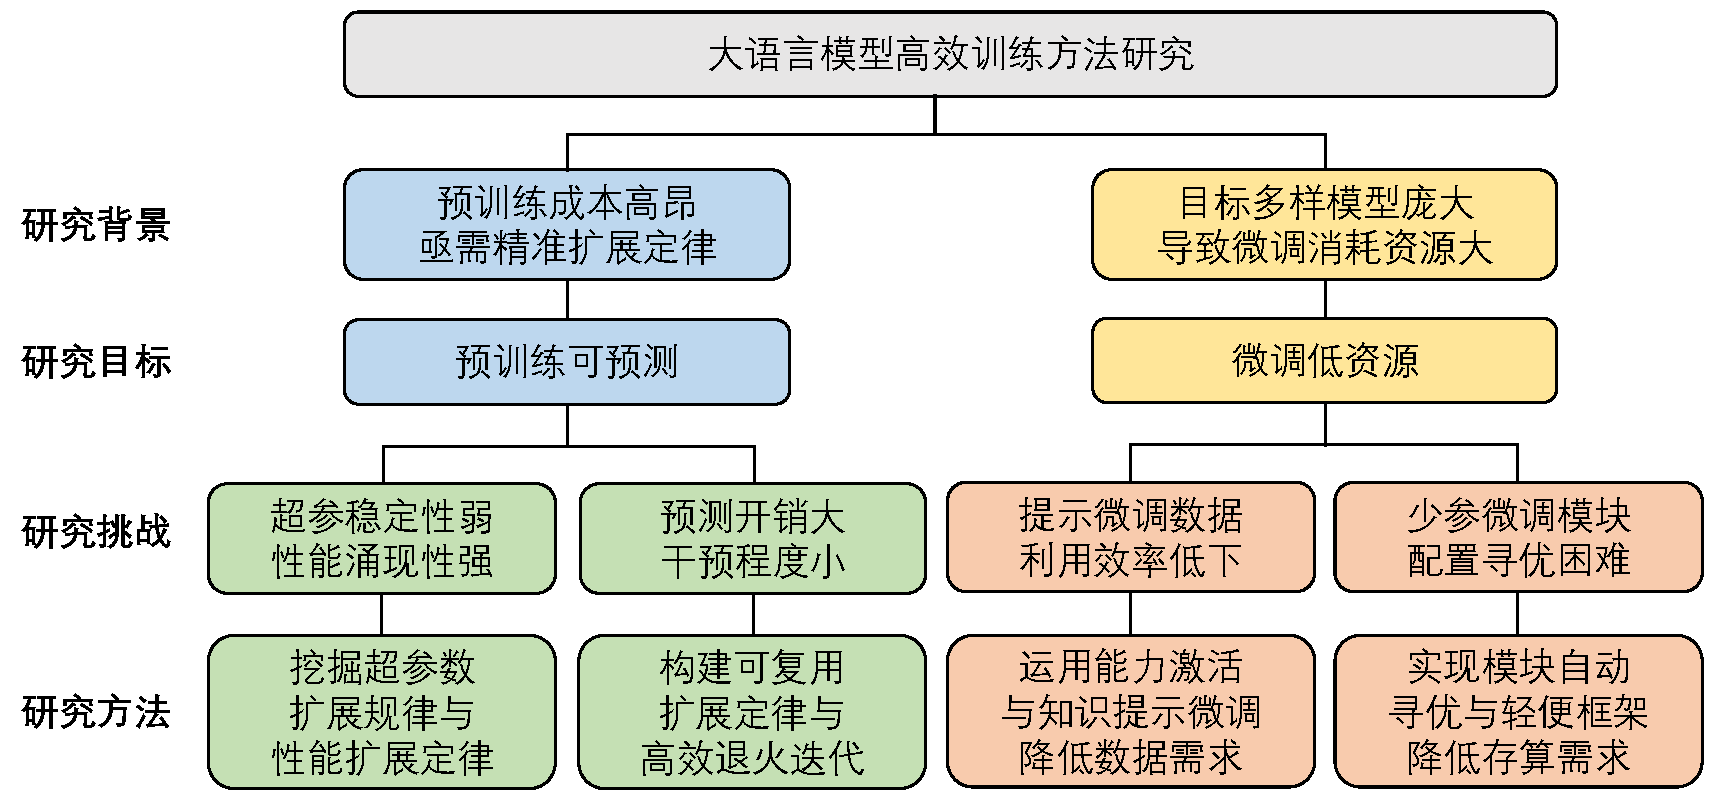
\includegraphics[width=\textwidth]{chap01/phdthesismain.pdf}
  \label{fig:mainframework}
  \caption{本文主要研究内容}
  \end{figure}

  
\subsection{面向可预测预训练的超参数扩展规律与性能扩展定律}
本研究首先基于Tensor Program~\cite{yang2022tensor}进行探索。Tensor Program中提出一种方法,希望通过对超参数的重参数化以及有理论保障的外推方法获得不随模型规模变化的稳定超参数。然而,Tensor Program并未在实践上证明对于真实场景的模型训练的有效性。本文在真实场景对Tensor Program进行了深入研究,发现在辅以批量大小的扩展方案时,可以获得稳定的学习率扩展规律。本研究还对其他一些结构变体,例如QK-Norm,是否能对超参数稳定起到关键作用进行了研究。

在得到了稳定的超参数扩展规律带来的损失扩展规律以后,本研究继续深入探索了性能扩展规律。性能扩展定律被认为是非常困难的。这是因为一个任务的性能不仅影响因素众多,而且还会表现出波动性和涌现性(被称作涌现能力)。前人的研究主要集中在对涌现能力的定性研究,并认为由于这种涌现能力的存在,导致任务性能无法预测。针对这个问题,本研究进行了深入实验,提出一种基于大量采样的提升模型评估分辨率的方法,我们证明了这一方法是真实表现的无偏估计,并且如果计算资源允许,可以精确到任意精度。我们进一步提出了性能扩展定律,区别于损失扩展定律,该定律可以直接对下游任务性能进行预测。我们进一步引入了数据集级别扩展和样本级别扩展两种方案,并且提出损失辅助预测方法。这些方法将性能预测精度提升到99\%以上,初步解决了性能扩展规律的问题。

\subsection{面向可预测预训练的可复用扩展定律与高效退火迭代}
本研究首先分析了进行扩展定律拟合过程中的资源消耗,发现现有文献的拟合方法需要消耗的计算量和拟合模型参数规模和数据规模都成线性关系,因此在数据和模型两个维度的扩展定律研究需要消耗平方复杂度的算力。本研究思考了不同数据量下的模型训练无法复用训练过程的原因,将其归结为学习率调度对损失的影响带来的不可复用性。本研究分析了当前绝大部分模型训练都使用的学习率调度策略,提炼出其效果优异的原因,即同时具备全局最优解寻找和局部最优解寻找(退火)的特点。本研究提出将占训练过程绝大部分时间的全局最优解进行多模型共享,再通过时机各异的局部最优解寻找来完成模型训练。本研究证明,这种方法使数据维度的扩展定律拟合消耗的资源变为常数量级,有效提高了扩展定律拟合过程的高效性。

本研究进一步实验指出,基于以上策略的扩展定律拟合方法,由于其可复用的退火阶段,使得高质量数据迭代实验变得非常高效。本研究仔细研究了退火过程中引入不同数据对于模型训练结果的影响。发现在退火过程中引入高质量数据能显著提高模型在下游任务上的表现。由于可复用的退火阶段在整个训练过程占比很小,所以可以使用少量的算力进行多次性能迭代。除此之外,本研究还探索了退火迭代的训练动力学方面的原因,为后人对训练机理的探索~\cite{wen2024understanding}提供了新的方向。本研究综合利用上述方法,利用1/7的算力和1/3的模型大小,训练了性能超越Llama2-7B的模型,证明了本研究方案的有效性。

\subsection{面向少资源微调的能力激活与知识激活}
本研究从微调阶段的数据角度出发,首先研究了对于预训练模型在分布外任务上,是否可以使用少量数据习得。本文以一类名为“错误先验立场”的问题入手。该类问题的特点是回答该类问题的知识存在于大语言模型的预训练阶段,但是由于分布的差异导致模型无法有效调用这些知识进行回答。我们第一次提供了精标注的人类对“错误先验立场”问题的回答,我们证明,只需要百到千量级的数据,就可以将模型的回复正确率从随机提升到接近90\%的准确率。这一发现提供了“小数据激活大能力”的有力证据,该思路也在后续的Instruction Tuning以及RLHF等工作中得到了进一步验证。

本研究进一步探索了对于与预训练模型能力更为接近的分布内任务,例如情感分类和主题分类,是否可以通过更少量的样本或者零样本来进行适配。知识微调是大模型范式下的有效适配手段,其利用模板和表达器来完成模型训练分布到任务输入输出空间的变换。本研究进一步提出了知识提示微调的概念,即在提示微调的基础上,引入知识库扩充的表达器,使得模型在微调过程中可以更好地利用预训练模型的知识。本研究指出通过在提示微调的表达器中引入人类知识先验,能够将模型性能提升高达17\%。

\subsection{面向少资源微调的参数高效微调模块自动化寻优}
本研究从微调阶段的存算资源角度出发,研究了参数高效微调的自动化模块选择功能。传统参数高效微调的方法会选择默认模块进行微调。尽管这种方法能够大幅减少需要微调的参数量,但由于在预训练过程中,不同模块已经训练出不同的分工,微调时使用默认模块可能会导致模型性能不能充分发挥。本研究提出了一种基于自动化模块选择的参数高效微调框架,该框架建立在对所有参数高效微调方法的统一建模视角下,借鉴了神经架构自动搜索算法,并创新地提出了可训练硬稀疏化优化目标,精准控制可微调参数总量。本研究使参数高效微调所需的微调参数量从全参数的1\%进一步降低到1\%\%量级(本文统一用\%\%表示万分之一),大幅减少了存算资源需求。



\section{本文组织结构}
本文共分为七章,其中第一章(即本章)为引言,主要介绍了本文的研究背景、研究意义、研究内容和主要贡献。第二章为相关工作,主要介绍了与本文研究内容相关的国内外研究现状和发展动态。第三章为预训练阶段的高效训练方法的第一部分,主要介绍超参数扩展规律和性能扩展规律,第四章为预训练阶段的高效训练方法的第二部分,主要介绍可复用扩展定律和高效退火迭代。第五章为微调阶段的高效训练方法第一部分,主要介绍了能力激活与知识提示微调。第六章为微调阶段的高效训练方法第二部分,主要介绍了模块自动化寻优的参数高效微调框架。第七章为总结与展望,主要总结了本文的研究工作,并对未来的研究方向进行了展望。


% !TeX root = ../thuthesis-example.tex

\chapter{研究现状与相关工作}

上一章总体介绍了大模型训练和微调过程中面临的效率挑战,本章将介绍大模型高效性研究的发展现状和相关工作。


\section{Transformer架构}
自然语言处理领域的革命性突破始于2017年Transformer架构~\cite{Vaswani+2017}的诞生。这个由Vaswani等人提出的创新架构,彻底改变了传统序列建模的范式。其核心设计摒弃了循环神经网络(RNN)的时序依赖特性,转而采用全局注意力机制,这使得模型能够并行处理整个文本序列,训练效率提升至数十倍。当前最大规模的GPT-4~\cite{openai2023gpt4}、PaLM~\cite{chowdhery2023palm}等万亿参数模型,均建立在此基础架构之上。

% \begin{figure}
% \centering
% 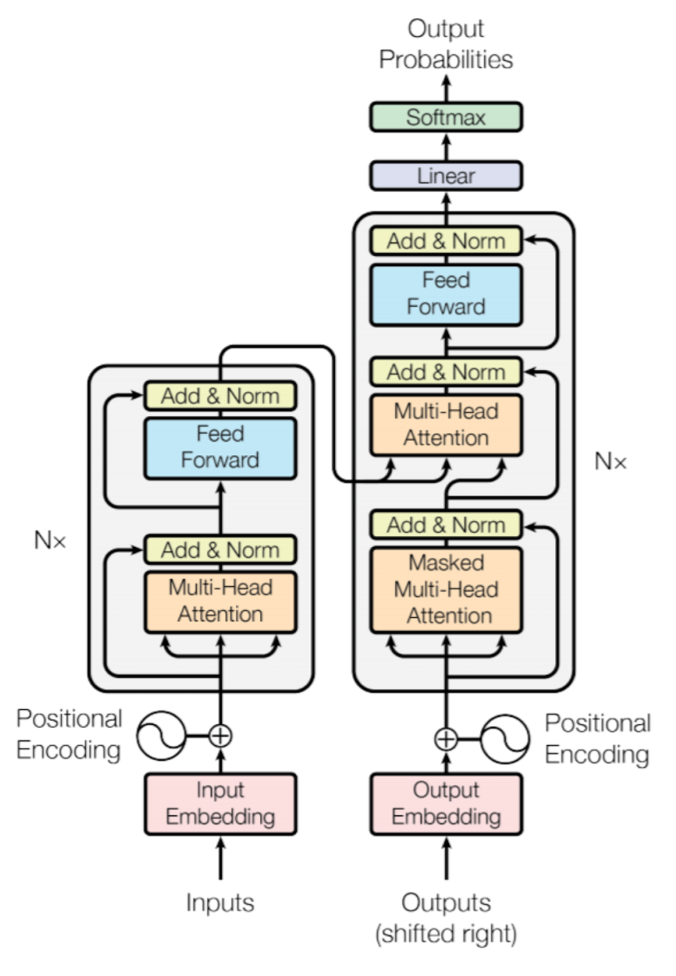
\includegraphics[width=0.5\linewidth]{misc/transformer.png}
% \caption{Transformer模型架构图}
% \label{fig:transformer}
% \end{figure}

每个Transformer层由两个关键模块协同工作:注意力机制与前馈网络。这种设计实现了对文本语义的多维度解析——注意力机制捕捉词语间的动态关联,前馈网络则负责特征的深度非线性转换。

\paragraph{注意力机制}
基础的注意力机制将输入$X$经过不同的线性变换转换为三种张量$Q=XW_Q$,$K=XW_K$,$V=XW_V$,然后通过($Q$,$K$,$V$)三元组运算建立关联。其数学表达为:

\begin{equation}
    \text{Attention}(Q, K, V) = \text{Softmax}(\frac{QK^T}{\sqrt{d_h}})V
\end{equation}
其中$d_h$是$Q$、$K$、$V$ 表示的隐藏维度,归一化因子$\sqrt{d_h}$的引入有效缓解了高维空间中的梯度消失问题。

自注意力机制的精妙之处在于让输入序列自我参照。通过线性投影矩阵$W^Q$、$W^K$、$W^V$从输入表示$X$中生成差异化的特征空间,使得同一词语能同时承担查询者与被查询者的双重角色。这种设计使得模型可以建立跨越整个文本的语义关联,例如在“bank”的词义消歧中,模型能同时关注到河流或金融方面等上下文含义。

Transformer中还引入了多头注意力机制。将$d_{model}$维的嵌入空间分割为$h$个独立子空间(通常每个子空间的维度为64或者128),每个头学习不同的关联模式。这种设计类似于卷积神经网络中的多通道概念,允许模型并行捕获语法、语义、指代等不同类型的语言特征。其输出通过可学习的投影矩阵$W^O$实现特征融合,保证了维度的一致性。

\paragraph{前馈网络}
标准的双层前馈网络(FFN)通过激活函数实现特征变换:
\begin{equation}
    \text{FFN}(x) = \text{ReLU}(xW_1 + b_1)W_2 + b_2
\end{equation}
后来的研究者提出了门控前馈网络,在上述基础上引入门控机制:
\begin{equation}
    \text{GLU}(x) = (xW_1 \odot \sigma(xW_2))W_3
\end{equation}

其中$\sigma$代表激活函数,这种设计增强了模型对特征重要性的调节能力,在同等参数量下提升了模型性能。

本文建立于Transformer架构基础上,主要研究该架构下的高效预训练和微调方法。

\section{训练范式}
现代大语言模型的训练遵循“预训练+微调”的两阶段范式。这一范式随着BERT~\cite{devlin2018bert}、GPT~\cite{radford2018improving}、T5~\cite{raffel2020exploring}等模型的流行变成主流~\cite{xu2021pre}。预训练范式在历史上出现过多种,例如:
\begin{enumerate}
    \item 自回归预测(GPT系列):基于上文逐词预测,采用单向注意力掩码,适合文本生成任务;
    \item 掩码语言建模(BERT系列):随机遮蔽$15\%$的输入词元(token),利用双向上下文进行预测,擅长语义理解;
    \item 混合目标训练(T5、BART~\cite{lewis2019bart}):结合文本修复、句子重排等多种预训练任务,增强模型鲁棒性。
\end{enumerate}
现在比较主流的是第一种,即自回归预测,方式简单通用,接近自然语言交互模式。

在预训练过程中,模型在TB量级的词元化(tokenized)数据上进行大规模预训练,每一次大规模预训练都将花费巨量开销,因此训练次数的稀缺性成为了调整模型性能的瓶颈之一。而在预训练之后,模型会被微调,以适应下游任务。由于下游任务种类众多,并且通常在应用端进行,微调用户不具备大规模算力。本文在“预训练+微调”范式的两个阶段都做了相应的创新,以实现全流程的高效训练。

\section{损失扩展定律}
大量的深度学习训练都被观察到有所谓“扩展”现象\citep{hestness2017deep, kaplan2020scaling, rae2021scaling, aghajanyan2023scaling}。文献\citet{hestness2017deep}研究了基于循环神经网络(RNN)模型中损失的幂律扩展行为。\citet{kaplan2020scaling}描绘了基于Transformer的语言模型的损失扩展趋势,并探究了最优超参数的扩展行为。他们正式确立了如下扩展定律:
\begin{equation}
\label{eq:loss_scaling_law}
    L = c N^{-\alpha} + L_0
\end{equation}
其中\(N\)是模型(在他们的研究范围内特指语言模型)的非嵌入参数数量,\(c\)、\(\alpha\)为正系数,\(L_0\)是代表数据中随机性的不可约损失。这一公式推动了大语言模型的参数扩展。随后,针对各种领域和场景都建立了扩展定律,包括多模态\citep{henighan2020scaling, zhai2022scaling}、计算受限场景\citep{hoffmann2022training}、数据工程\citep{muennighoff2023scaling,sorscher2022beyond}以及强化学习\citep{gao2023scaling}等领域。\citet{yao2023research}通过引入超参数扩展方法,将该扩展定律扩展到跨超参数的损失预测领域。本文与现有文献存在两方面的联系。其一,这些文献主要聚焦于训练和验证时的损失指标,而这些指标并不能可靠地预测任务性能。本文基于这些扩展定律,扩展到任务性能的扩展定律。其二,本文第一次在大规模预训练场景下验证包含超参数扩展规律的全面扩展定律。


\section{任务性能的扩展行为}

尽管大语言模型的损失呈现可预测的下降趋势,但在模型扩展过程中,任务性能的提升却并非一帆风顺。虽然一些主要依赖知识记忆的任务呈现出逐步提升的态势,但随着模型规模的增大,众多任务展现出“涌现”能力\citep{srivastava2022beyond,wei2022emergent},即随着模型规模扩大,达到某一定阈值时,一些关键能力取得突飞猛进的进展。\citet{wei2022emergent}表明,“涌现”这一概念同样适用于诸如思维链\citep{wei2022chain}和上下文学习\citep{brown2020language}等提示学习技术,这使得理解任务性能的扩展定律变得更加复杂。似乎损失扩展定律并不能保证任务性能的提升,在预训练方法上也缺乏指导意义。
有几项研究致力于揭开这些涌现能力的神秘面纱。GPT-4的技术报告\citep{openai2023gpt4}称,GPT-4的任务性能可以用不到万分之一的计算量进行预测,不过并未披露具体方法,且承认某些能力仍然无法预测。另一项研究\citep{schaeffer2023emergent}将涌现归因于两个方面。第一个原因是非平滑指标导致的性能离散变化。本文对此并不认同,因为替代指标无法解释像精确匹配这样研究者最为关注的目标指标的突然提升。本文认同他们的第二个归因,即通过增加更多测试样本来提高分辨率。与他们的方法不同,本文提出了一种无需增加测试样本就能提高分辨率的实用方法。本文也是首次在开源环境下对任务性能的扩展行为进行定量研究的尝试,提出了任务扩展定律和加速涌现现象。 

\section{可扩展的预训练策略}

自从扩展定律\citep{hestness2017deep, kaplan2020scaling, rae2021scaling, aghajanyan2023scaling}被发现以来,人们从不同角度追求科学且可预测地\citep{achiam2023gpt,hu2023unlock, du2024understanding}扩大大语言模型的规模,尤其是在预训练阶段。预训练阶段容易有训练不稳定现象,为此,前人提出了张量程序(Tensor Program)系列工作\citep{yang2022tensor, yang2023tensor},以确保在不同模型规模下超参数的最优一致性。这种技术被用在训练CerebrasGPT\citep{dey2023cerebras}中。此外,\citet{wortsman2023small}建议利用较小的模型来预测并减轻较大模型训练中的不稳定性。从训练数据的角度来看,人们倡导了各种以数据为中心的策略\citep{xie2024doremi, shi2023context, ye2024data}。在训练方法领域,先前的研究深入探讨了各种学习率调度器(Learning Rate Scheduler)\citep{howard2018universal, raffel2020exploring, hundt2019sharpdarts},其中余弦退火学习率调度器(Cosine LRS)\citep{loshchilov2016sgdr}成为大语言模型中的主要选择。\citet{kaplan2020scaling,hoffmann2022training}精心研究了余弦退火学习率调度器的超参数,从而为后续的预训练工作奠定了基础。也有一些工作采用了非余弦退火学习率调度,例如DeepSeek\citep{bi2024deepseek}与本文提出的WSD学习率调度器有一定相似之处。关于批量大小调度,\citet{smith2017don}主张增加批量大小作为降低学习率的替代方法,这也是Yi-9B\citep{young2024yi}采用的策略。

\section{小规模语言模型}

本文使用多种可预测预训练技术,利用较少的资源预训练了一个小规模语言模型 (2.4B参数规模),其效果超过同期的Llama2-7B~\cite{touvron2023llama2},比肩Mistral-7B~\cite{jiang2023mistral}。
所谓“小语言模型”(SLMs),是一个不断演变的概念,随着时间推移经历了重大变革。目前,小语言模型通常被理解为与知名大语言模型相比规模较小的模型,其参数一般不超过70亿。这些模型的特点是能够在终端用户设备(如个人电脑和智能手机)上部署,即便没有图形处理器(GPU)也能运行。当前小语言模型领域的典型例子包括Phi系列\citep{gunasekar2023textbooks, li2023textbooks, Javaheripi2023Phi2}、TinyLlama\citep{zhang2024tinyllama}、MobileLLM\citep{liu2024mobilellm}以及Gemma\citep{Banks2024Gemma}等。 人们探索了多种方法来提高小语言模型的性能。这些方法包括使用高质量数据\citep{gunasekar2023textbooks, li2023textbooks, Javaheripi2023Phi2}、应用结构剪枝技术\citep{xia2023sheared},以及重新配置模型架构\citep{liu2024mobilellm}等。本文通过精心整合超参数优化、策略性训练方法、架构设计以及高质量数据,完成了小规模语言模型的高效训练。


\section{提示学习}
自从GPT-3~\cite{brown2020language}出现以来,提示学习(prompt-learning)受到了广泛关注。  
GPT-3表明,通过提示调优和上下文学习,大规模语言模型在低数据量情况下也能取得优异的性能。  
后续的研究~\cite{schick2020exploiting, schick2020s}指出,小规模语言模型~\cite{radford2018improving, devlin2019bert, liu2019roberta, lan2019albert}通过提示调优也能取得不错的表现。提示调优已被应用于多种任务,例如文本分类~\cite{schick2020exploiting}、自然语言理解~\cite{schick2020s, liu2021gpt}、关系抽取~\cite{han2021ptr,chen2021adaprompt}以及知识探测~\cite{petroni2019language, liu2021gpt}等。

标签词是提示调优中的重要组成部分,对提示调优的性能有显著影响~\cite{holtzman2021surface, gao2020making}。大多数研究使用人工编写的标签词~\cite{schick2020exploiting},这些标签词往往带有个人词汇的偏见且覆盖范围不足。其他一些研究~\cite{gao2020making, shin2020autoprompt,liu2021gpt,schick2020automatically}设计了自动标签词搜索方法以寻找更好的标签词选择,但这些方法需要充足的训练集和验证集进行优化。此外,自动确定的标签词通常是类别名称的同义词,这与本文通过外部知识库扩展标签词以涵盖多样化且全面的标签词的直觉有所不同。  
~\citet{schick2020automatically}和~\citet{shin2020autoprompt}也尝试为每个类别使用多个标签词。  
他们的标签词集合的最优大小通常少于10个,这在文本分类任务中缺乏足够的覆盖性。

\section{参数高效微调}
随着模型规模指数级增长,全参数微调面临严峻挑战。主要挑战有三点:1. 计算成本不菲,微调175B参数的GPT-3需要数百张GPU的算力; 2. 储存成本高昂,储存微调后的大语言模型需要消耗和储存预训练模型一样大的空间开销;3. 过度微调会导致模型丧失通用能力,灾难性遗忘现象频发。在此背景下,参数高效微调(Parameter-efficient Tuning,又叫Delta Tuning~\cite{ding2022delta})应运而生。本文即与预训练模型的参数高效微调相关。参数高效微调只优化一小部分参数,而保留绝大多数参数不变,以低成本地适应下游任务。

早期的研究选择预训练模型进行部分微调~\cite{tajbakhsh2016convolutional, guo2020adafilter, guo2019spottune}。  
Adapter~\cite{houlsby2019parameter}是最早将参数高效微调方法应用于预训练语言模型的方法之一,它在每个Transformer层中插入线性神经模块,并取得了与全量微调相当的结果。  
随着近年来预训练语言模型规模的扩大,参数高效微调因其在计算和存储上的高效性而受到重视。这不仅催生了大量对Adapter的研究~\cite{pfeiffer2020adapterfusion,he2021effectiveness}
以及Adapter的变体~\cite{mahabadi2021compacter,sung2021vl},
还衍生出了一系列其他方法。  
Prefix tuning~\cite{li2021prefix}将嵌入向量附加到Transformer模型的隐藏状态前,而Prompt Tuning~\cite{lester2021power}进一步简化了这一策略,仅将此类嵌入向量附加到输入层。  
还有一些方法通过指定预训练模型中的部分参数为可训练参数来取得良好效果,例如Masking~\cite{zhao2020masking}、BitFit~\cite{zaken2021bitfit}、DiffPruning~\cite{guo2021parameter}等。另一流行的方法是LoRA~\cite{hu2021lora}。LoRA假设模型权重在微调后的变化本质上是低秩的,并使用可训练的秩分解矩阵进行模型微调。  
除了具体方法外,一些研究还对参数高效微调进行了探讨。~\citet{he2022unified}以统一的方式建模了多种方法,~\citet{ding2022delta}则提供了这些方法的理论讨论和全面的分析研究。  
本文提出在参数高效微调背景下的自动搜索可训练结构,这与上述所有工作的视角不同。在参数高效微调结构配置方面,AdapterDrop~\cite{ruckle-etal-2021-adapterdrop}基于手动试验探索了丢弃部分Adapter模块的方法。另一项工作~\cite{moosavi2022adaptable}通过在Adapter模块上学习开关来选择有益的Adapter模块,但该方法并未在预设的可训练参数数量下进行优化。此外,它们都局限于基于Adapter的方法。相比之下,本文提出的方法可以在受限的可训练参数预算下,在几乎所有参数高效微调模块的混合中进行搜索。  


\section{神经架构搜索} 

本文在参数高效微调范围内进行结构搜索,这与神经架构搜索算法(Neural Architecture Search, NAS)相关。一类NAS算法使用强化学习或进化算法,通过从头训练结构并获取奖励来探索最佳结构~\cite{zoph2016neural, zoph2018learning,real2019regularized,pham2018efficient},这种方法通常消耗大量的计算资源。另一类NAS算法~\cite{liu2018darts, liang2019darts+, chen2019progressive}通过基于梯度的优化来解决这一问题。DARTS~\cite{liu2018darts}使用连续结构参数对离散结构进行松弛化,并通过梯度下降的方法进行优化。DARTS以更少的计算资源取得了具有竞争力的性能。本文从DARTS中汲取灵感,优化了结构参数。本文也是第一个在预训练骨干模型条件下进行NAS的研究。此外,本文还从带有二值门的NAS算法中汲取了灵感~\cite{cai2018proxylessnas, wu2019fbnet}。



% !TeX root = ../thuthesis-example.tex

\chapter{可预测预训练--超参数可预测扩展}

% \pkg{natbib} 


在上一章中,我总体介绍了预训练技术以及可预测预训练技术的理念。在本章中,我将介绍本文可预测预训练技术的第一部分,即超参数可预测扩展技术。

\section{预训练超参数简介}

在深度学习模型的预训练中,超参数起着关键作用,直接影响模型的训练效率、性能表现以及最终的泛化能力。

\paragraph{参数初始化方案}
参数初始化是模型训练的起点,合理的初始化方案能够加速模型收敛,避免梯度消失或梯度爆炸等问题。常见的初始化方法包括随机初始化和基于特定分布的初始化。随机初始化通常是从均匀分布或正态分布中随机采样数值来初始化模型参数。例如,在神经网络中,权重矩阵可以通过均匀分布初始化,使每个参数在一定范围内取值,这有助于打破模型训练的对称性,防止所有神经元在训练过程中表现一致。
另一种常用的初始化方法是基于特定分布的初始化,如 Xavier初始化~\cite{pmlr-v9-glorot10a}和 He初始化~\cite{he2015delving}。Xavier初始化根据输入和输出神经元的数量来调整初始化参数的标准差,使得在正向传播和反向传播过程中,信号能够在各层之间较为均匀地传递,从而提高训练的稳定性。He 初始化则针对 ReLU 激活函数进行了优化,它能够更好地适应 ReLU 函数在负半轴输出为 0 的特性,使得模型在使用 ReLU 激活函数时能够更快地收敛。
在本章中,我们对参数初始化方案进行了调整,主要参考来自Tensor Program的初始化方案,结合实际大语言模型训练的实际情况,实现稳定的规模化。


\paragraph{批量大小(batch size)}
批量大小指的是在一次训练迭代中,用于计算梯度和更新参数的样本数量。较大的批量大小可以利用更多的数据信息来计算梯度,使得梯度估计更加准确,从而加速模型的收敛。然而,较大的批量大小也会带来更高的内存需求和计算成本,并且可能导致模型在训练过程中对某些样本的过拟合。
较小的批量大小可以在每次迭代中更快地更新参数,增加模型训练的随机性,有助于跳出局部最优解。但同时,由于每次使用的数据量较少,梯度估计的噪声较大,可能会导致模型收敛不稳定。在传统深度学习的训练中,需要根据数据集的大小、模型的复杂度以及硬件资源等因素来选择合适的批量大小。通常,可以通过实验来探索不同批量大小对模型性能的影响,从而找到最优的设置。然而在大语言模型训练中,没有办法在每次大规模实验前仔细调整批量大小,因此研究批量大小如何随着模型规模扩大变得很重要。

\paragraph{学习率}
学习率决定了模型在训练过程中参数更新的步长。如果学习率设置过小,模型的训练过程会非常缓慢,需要更多的训练轮次才能达到较好的收敛效果;而如果学习率设置过大,模型可能会在训练过程中无法收敛,甚至出现损失函数不断增大的情况。
常见的学习率调整策略包括固定学习率、学习率衰减和自适应学习率。固定学习率在整个训练过程中保持不变,适用于一些简单的模型和数据集。学习率衰减则是在训练过程中逐渐降低学习率,这样可以在训练初期快速更新参数,加速收敛,而在训练后期减小步长,避免错过最优解。常见的学习率衰减方法有指数衰减、余弦退火衰减等。在模型规模扩大过程做,最优的学习率不是通常不是一成不变的。在本章中,我们将结合多方调整,使最优学习率保持稳定。

\improvement{加一个Transformer图}

\section {参数初始化设置}
Tensor Program\citep{yang2022tensor, yang2023tensor} 提出了一个框架,用于稳定不同规模模型的超参数。Tensor Program 的主要部分是宽度缩放\citep{yang2022tensor} 和深度缩放\citep{yang2023tensor}。前者帮助 CerebrasGPT~\citep{dey2023cerebras} 更准确地预测大语言模型的损失。我们对这些技术进行了广泛尝试,有选择地使用了其中几种作为最终方案。

这些操作包括
\begin{enumerate}
  \item 嵌入层输出缩放:将嵌入层的输出乘以$\text{scale\_\text{emb}}$。
  \item 残差连接缩放:在将每个层的块的输出张量添加到每个残差连接之前,将其按$\text{scale\_\text{depth}}/\sqrt{\text{num\_layers}}$进行缩放。
  \item 张量初始化:将每个二维张量参数的初始化标准差设置为$\text{init\_std}/\sqrt{d_m/d_{base}}$,并将其他参数的初始化设置为0.1。
  \item 张量的学习率缩放:将每个二维张量参数的学习率调整为其他部分(或整体学习率)学习率的$1/({d_m/d_{base}})$倍。
  \item 语言模型头部缩放:将输出的对数几率调整为原始值的$1/(d_m/d_{base})$倍。
\end{enumerate}

由于在大语言模型的实际应用中,多注意力头的维度一般为64维,或者128维,而只会方法多注意力头的个数,因此处于这点考虑,本文没有应用~\citep{yang2022tensor} 中提出的注意力Softmax操作归一化因子的缩放技术技术。

与\cite{yang2023tensor}中不同之处在于,他们提出,对于深度大于 2 的网络,深度缩放并不令人满意,但我们通过实验发现得到的最优学习率是稳定的。

\subsection{贝叶斯超参数搜索}
该超参数的扩展方案进一步引入了三个模型大小无关超参数,为了确定这三个超参数,我们在一组预定义的参数空间上进行了广泛的贝叶斯搜索。我们针对 $N = 0.009B$ 的模型进行搜索。为了进一步减少实验需要的资源,在前期实验中,我们证实,当使用规模为 $10N$ 和 $20N$ 数量级的数据集进行超参数优化时,超参数的有效性呈现出一致性。因此,我们使用 $|D| = 10N = 0.09B$ 个词元(tokens)来训练模型。

同时,我们还尝试了QK - Norm~\citep{henry-etal-2020-query}和独立权重衰减~\citep{loshchilov2017decoupled},以稳定学习率。整体结果如图\ref{fig:mupsearch_app}所示。应用QK-norm后,我们观察到学习率敏感性显著降低,这与~\cite{wortsman2023small}的情况类似。根据图\ref{fig:mupsearch_app}中,我们确定了最佳超参数为 $scale\_depth = 1.4$,$scale\_emb = 12$,$init\_std = 0.1$ 以及 $lr = 0.01$。


\begin{figure}[htbp]
  \centering
  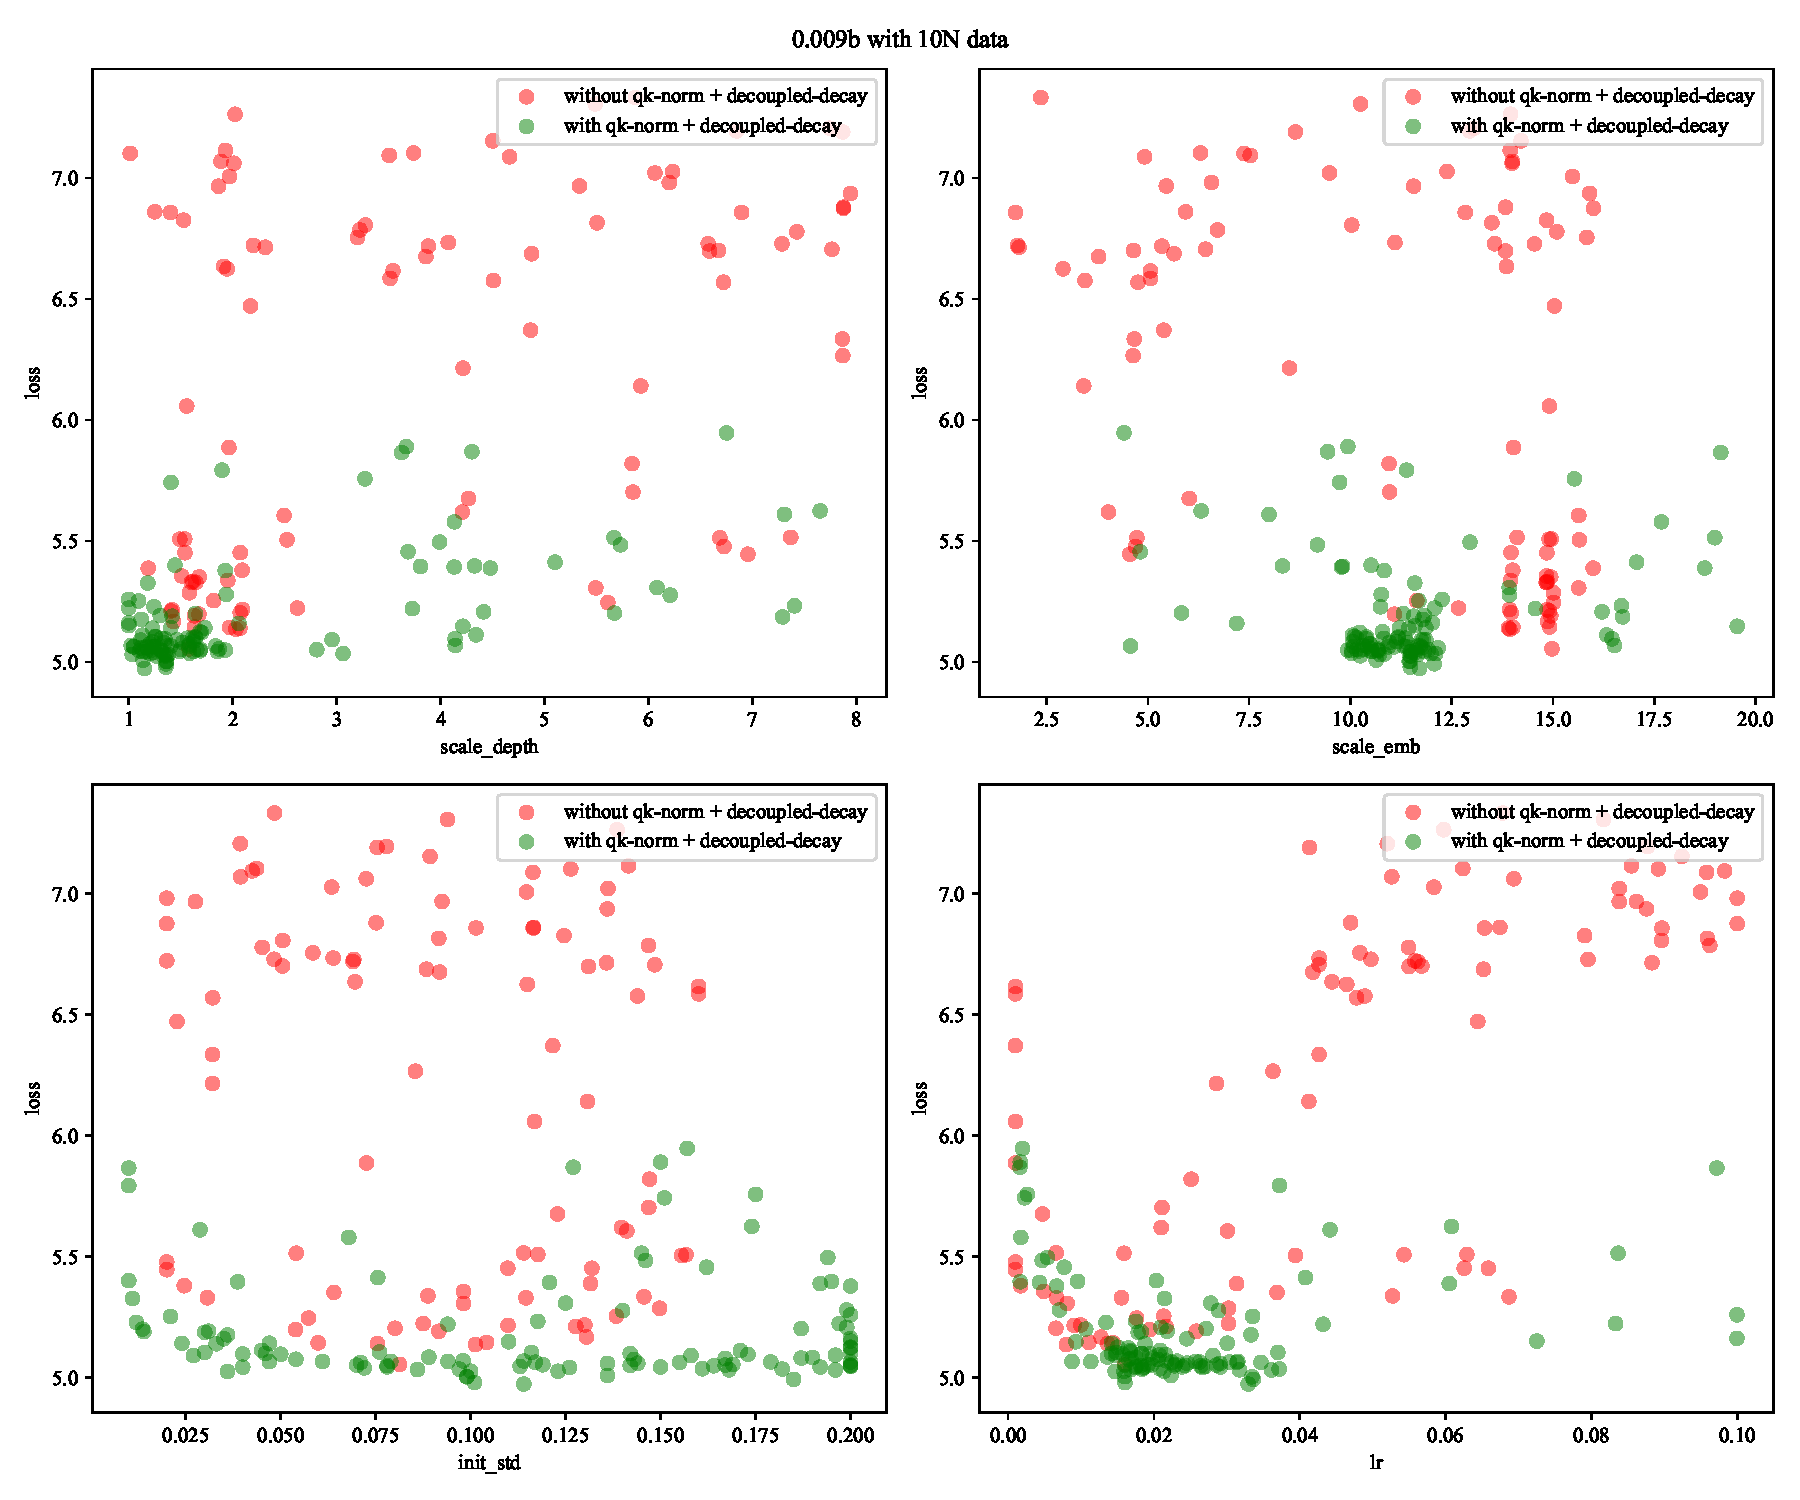
\includegraphics[width=\linewidth]{chap03/mup0.009bwith10Ndata.pdf}
  \caption{Grid search over the $\mu$P parameterization spaces.}
  \label{fig:mupsearch_app}
\end{figure}

\section{最优批量大小}

批量大小决定了模型收敛速度与计算资源消耗之间的平衡。如果批量大小过大,将导致大量的数据和计算成本。另一方面,如果批量大小过小,则需要大量的训练步骤,并且可能导致损失函数的下降有限。我们遵循~\cite{kaplan2020scaling} 从预期损失确定批量大小的方法,并对其设置做了轻微修改。


在~\cite{kaplan2020scaling}中,OpenAI研究了损失函数与token数量之间的关系。在他们的实验中,他们假设消耗更多的步骤等同于消耗更多的时间。在这一假设下,OpenAI定义了一个关键批量大小,该批量大小可以在不消耗过多步骤或token的情况下实现一定的损失。如果实验提供了无限的GPU(至少在实验范围内),这一理由是有效的。由于GPU是无限的,增大批量大小不会增加单步时间,但会减少总步骤数。然而,在我们的实验中,由于我们拥有固定的资源(GPU数量),我们观察到将批量大小翻倍几乎等同于将单步时间翻倍。因此,通过增大批量大小来减少总训练步骤对总训练时间的影响微乎其微。基于这一观察,我们放弃了“不消耗过多步骤”的目标,转而专注于最小化token数量以实现最低损失。

关于最优批量大小与损失之间关系的估计类似于“鸡与蛋”悖论。实际上,通常可以通过初步实验的先验知识对给定模型大小下可实现的损失进行初步估计。然而,未来有可能开发出更精细的估计方法。

最优批量大小和最优学习率可能并不是独立的。为了克服这种相关性,我们首先对学习率进行了初步研究,然后选择一个最优学习率进行批量大小实验,并使用批量大小缩放再次调整学习率。这有点类似于坐标下降优化方法。然而,未来的工作中欢迎更严格的方法。


为实现这一目标,我们分别在 0.09 亿、0.3 亿和 1.7 亿参数规模的模型上进行实验。每个模型规模在全局学习率为 0.01 且使用余弦退火学习率调度器的情况下,在 6 种批量大小下进行训练。我们观察了在 C4~\citep{2019t5} 数据集上最优批量大小随损失的变化趋势(图 \ref{fig:optimalbatchsize} 中的红线)。

\begin {figure}[!htbp]
\centering
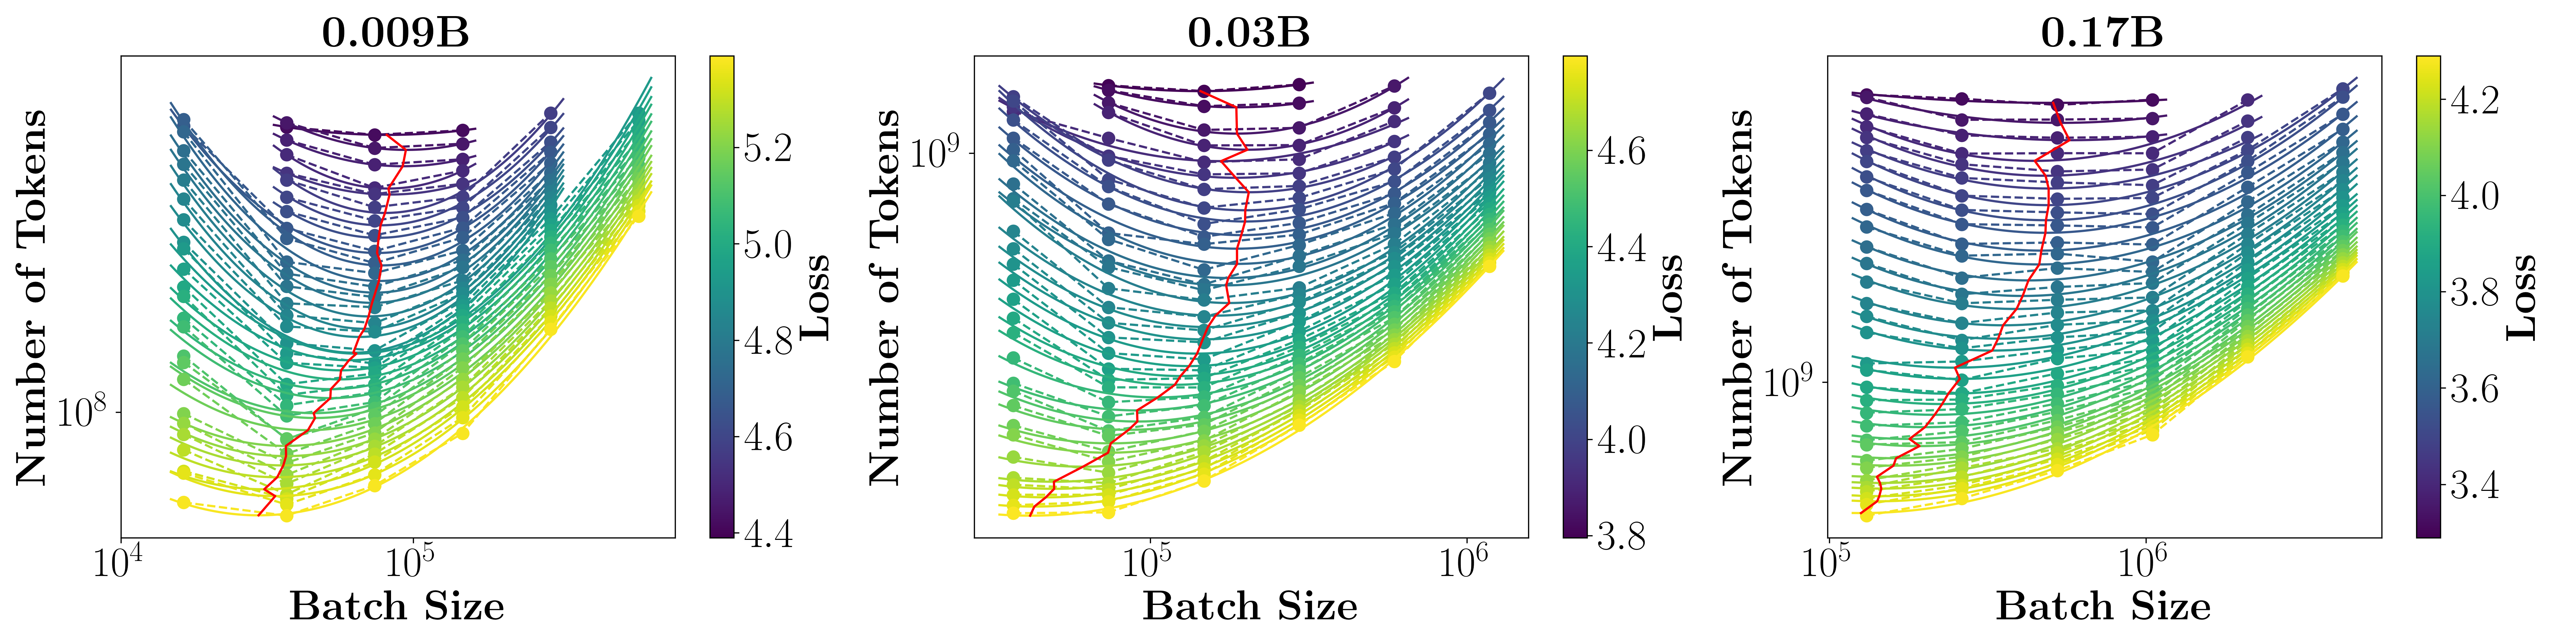
\includegraphics [width=\linewidth]{chap03/batch_size_1.png}
\caption {我们展示了三种不同规模模型在不同批量大小下训练的损失曲线。由具有渐变颜色的点形成的每条垂直线代表一条训练曲线。颜色越浅表示损失越高。}
\label {fig:optimalbatchsize}
\end {figure}


\begin {figure}[!htbp]
\centering
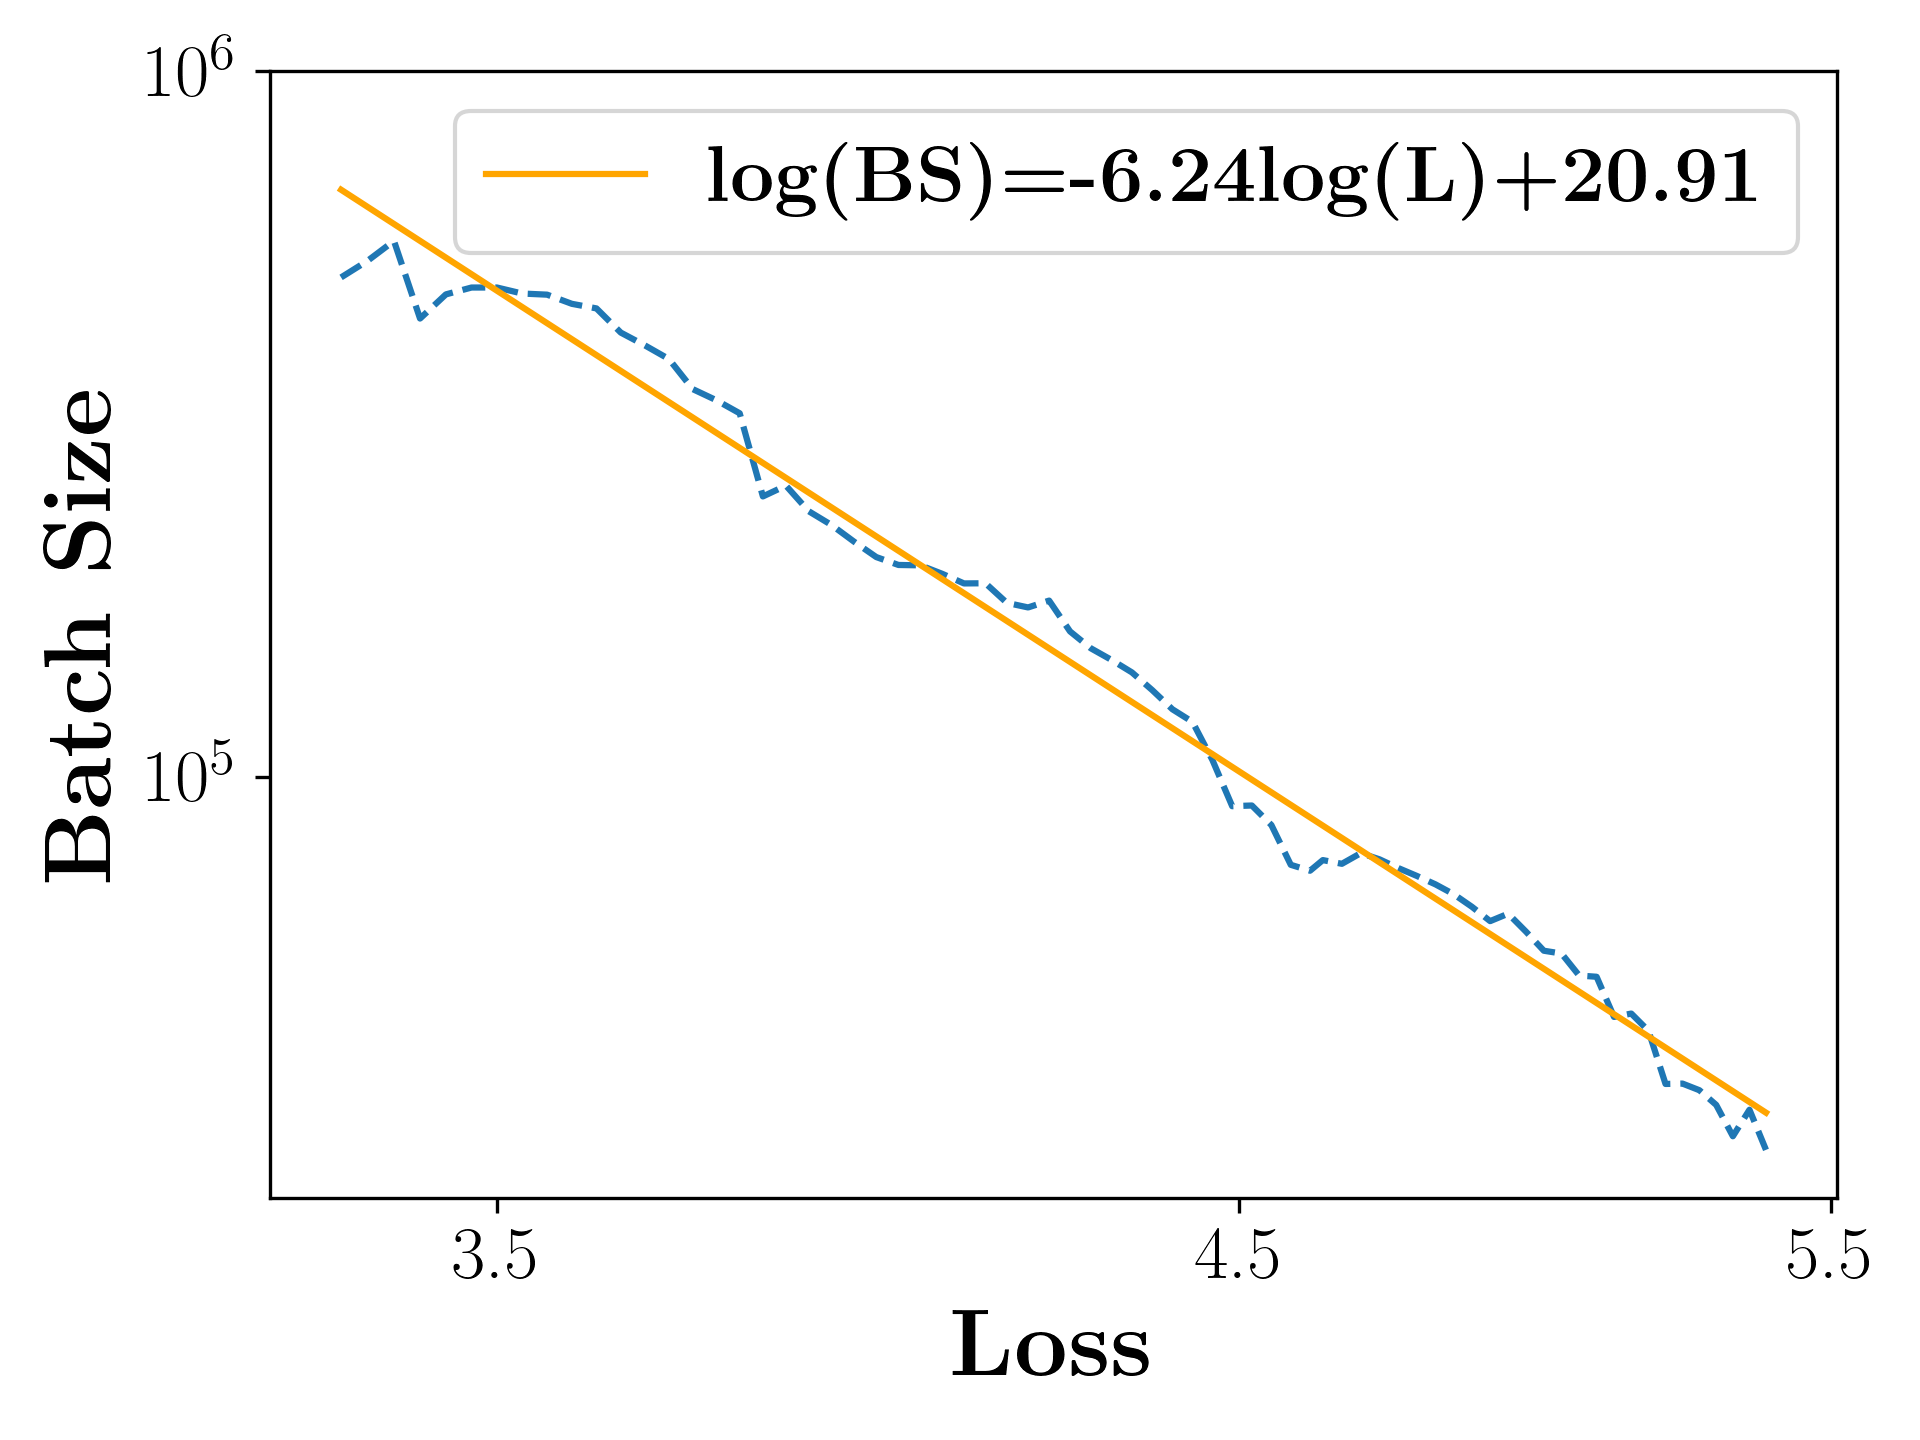
\includegraphics [width=\linewidth]{chap03/batch_size_2.png}
\caption {相连的最优批量大小。 }
\label {fig:optimalbatchsizeconnect}
\end {figure}


如图 \ref {fig:optimalbatchsize} 所示,我们将批量大小绘制在 x 轴上,token 消耗绘制在 y 轴上,点的颜色代表损失。因此,由带颜色的点形成的垂直线表示一条训练曲线。我们使用抛物线拟合等损失点,并用红线连接抛物线的最小值。这些线表明随着损失降低,最优批量大小向更大值移动。然后我们连接这三条线(见图 \ref {fig:optimalbatchsizeconnect}),发现在对数空间中这些线很好地连接成一种线性关系,由此我们得到批量大小与 C4 损失之间的以下关系:$ bs = \frac{1.21\times10^9}{L^{6.24}}$。

\section {最优学习率}
由于我们使用了 Tensor Program~\citep{yang2022tensor, yang2023tensor},我们预计在模型缩放过程中学习率不会发生显著变化。为了验证这一点,我们在 0.4 亿、1 亿、3 亿和 5 亿参数规模上进行了六组学习率实验。在图 \ref {fig:loss_vs_lr} 中,我们发现尽管模型规模增加了十倍,但最优基础学习率 \footnote{二维张量的实际学习率将根据 Tensor Program 进行缩放。} 并没有明显变化,仍保持在 0.01 左右。我们进一步在 21 亿参数规模上进行了简单验证,证实学习率为 0.01 确实能达到最低损失。

\begin{figure}[htbp]
  \centering
  % First minipage for the first figure
      \centering
      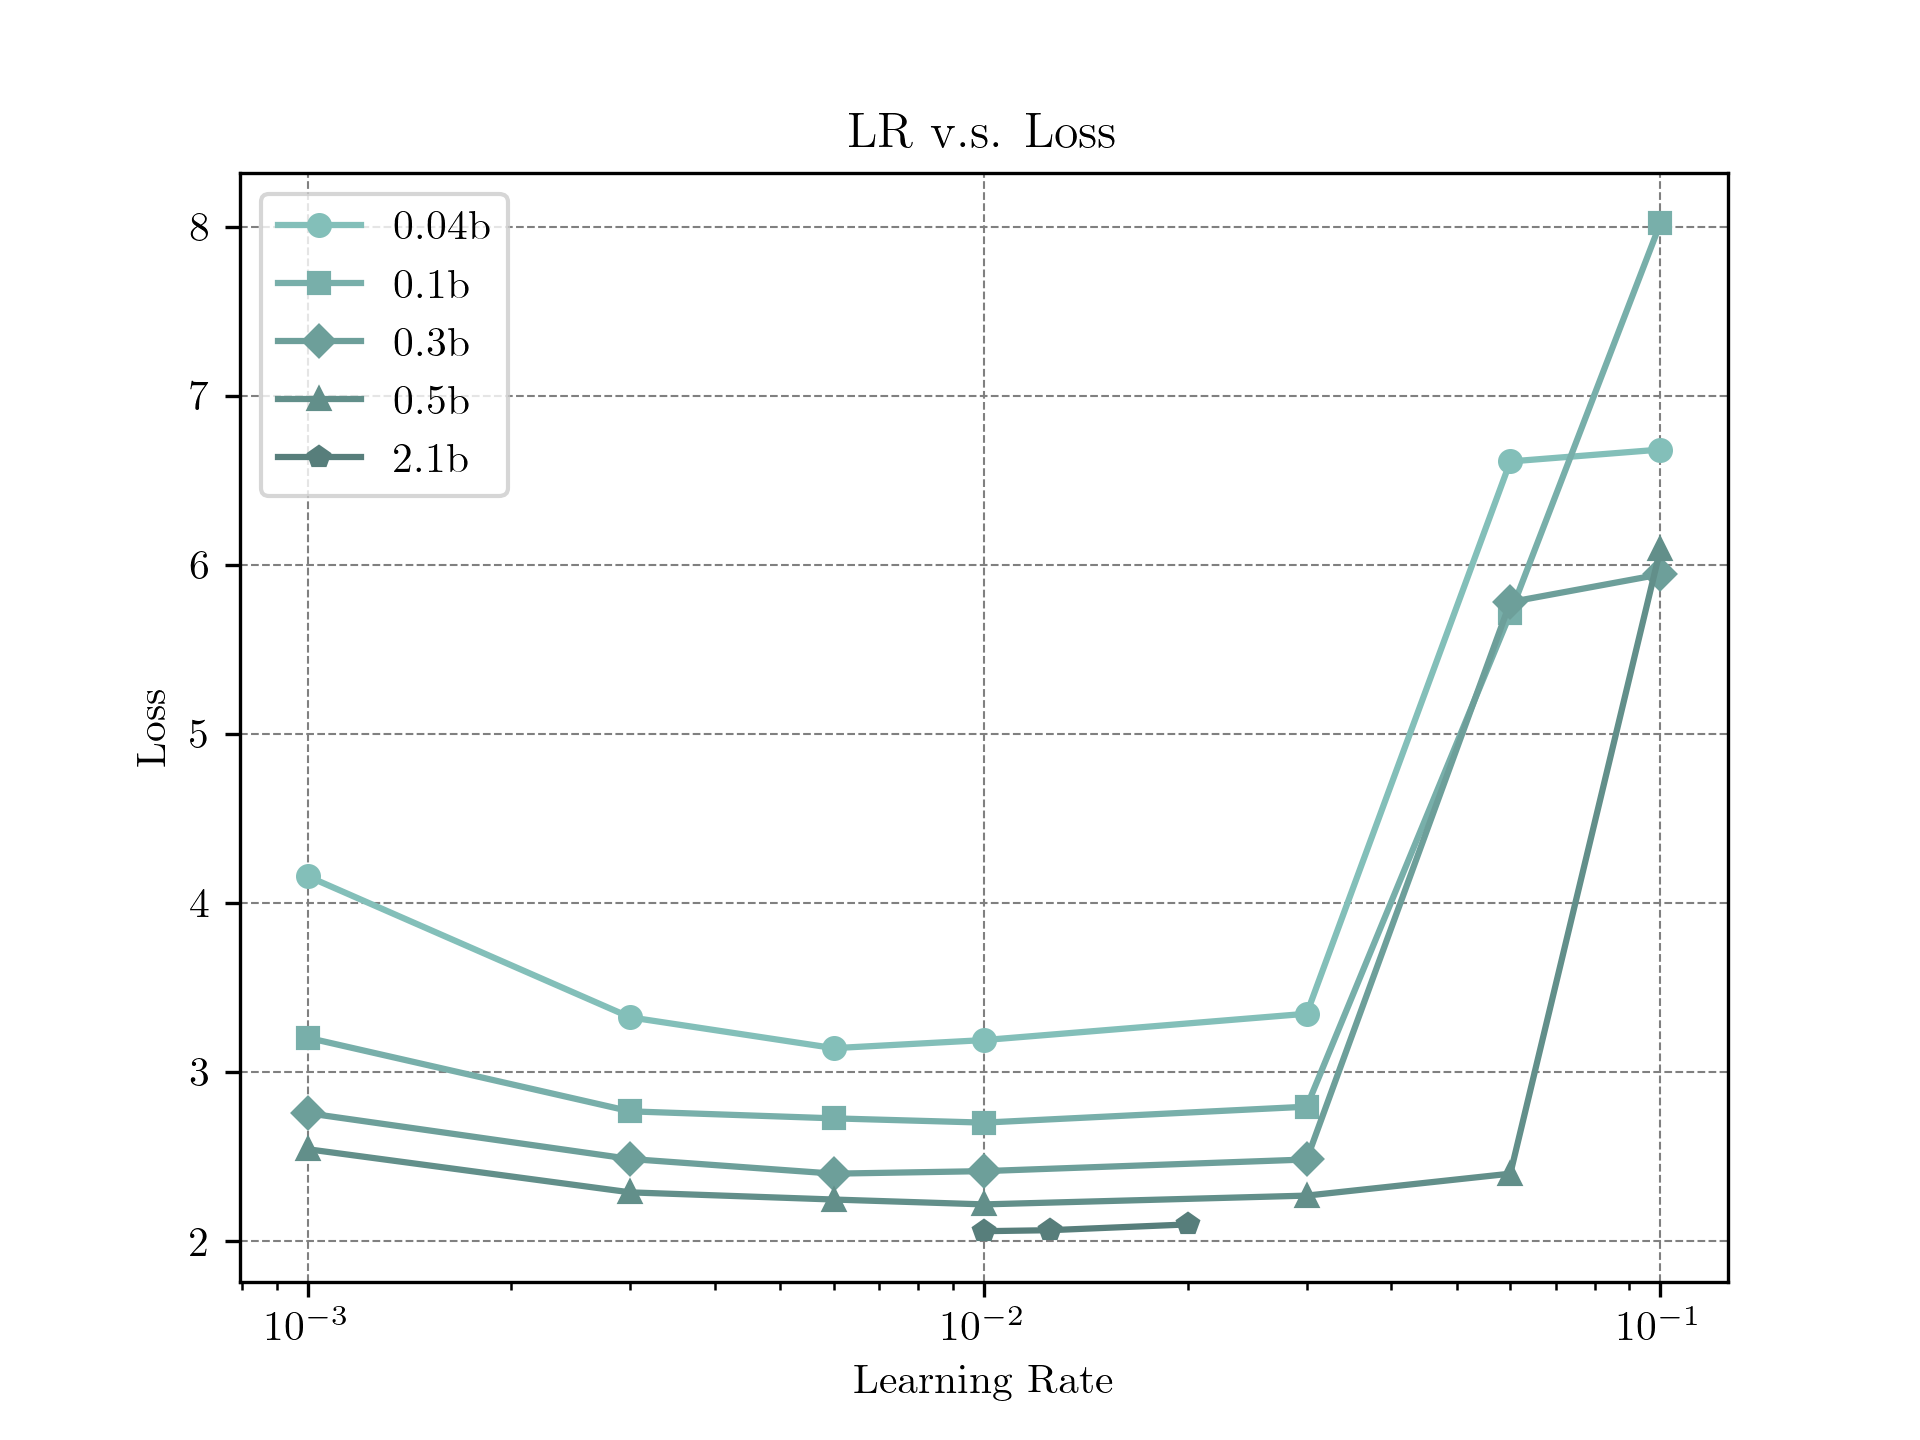
\includegraphics[width=0.9\linewidth]{chap03/loss_vs_lr.png}
      \caption{损失关于学习率的变化图像。在Loss vs Learning Rate. After applying for the Tensor Program, the learning rate shift becomes minimal.}
      \label{fig:loss_vs_lr}
\end{figure}

  % Second minipage for the second figure
%   \begin{minipage}{0.46\linewidth}
%     \centering
%     \includegraphics[width=1.0\linewidth]{Fig/cosine_2024-03-26_15-36-16.pdf}
%     \caption{Cosine Learning Rate Scheduler with different periods. The Y-axis is the loss on the C4 corpus.}
%     \label{fig:cosine_lr}
%     \vspace{0.47cm}
% \end{minipage}
% \end{figure}
% \vspace{-5mm}

\section{实验配置}
在表~\ref{tab:appmodel_configs}中列出了在模型规模扩增实验中使用的模型配置。力图让模型的“形状”,即模型宽度与模型深度的比例,尽可能保持一致,以避免任何潜在的性能变化。

\begin{table}[htbp]
    \centering
    \begin{tabular}{c|cccccc}
    \toprule
        \textbf{名称} & \textbf{N (B)}& $d_m$ & $d_{ff}$ &$d_h$ & $n_h$ & $L$ \\
    \midrule
          9M    &  0.009 & 320 & 800 & 64 & 5 & 8\\
           30M &   0.036 & 512 & 1280 & 64 & 8 & 12  \\
          70M &  0.066 & 640 & 1600 & 64 & 10 & 14\\
          0.1B &  0.109 & 768 & 1920 & 64 & 12 & 16  \\
         0.17B &  0.166 & 896 & 2240 & 64 & 14 & 18 \\
         0.2B&  0.241 & 1024 & 2560 & 64 & 16 & 20 \\
        0.5B& 0.499 & 1344 & 3360 & 64 & 21 & 24 \\
    \bottomrule
    \end{tabular}
    \caption{缩放曲线中模型的配置和训练配置。N(B)表示模型的非嵌入参数数量,单位为十亿。
    % BS(M)表示用于训练模型的批次中的token数量(即批量大小),单位为百万。TS表示训练步数。Tokens(B)表示用于训练模型的总token数量。
    }
    \label{tab:appmodel_configs}
\end{table}
% !TeX root = ../thuthesis-example.tex

\chapter{可预测预训练--基于新型学习率调度的可预测性扩展}
% \thusetup{
%   cite-style = super,
% }

在上一章中,我介绍了使用超参数可扩展策略进行大语言模型预训练,节省模型的超参调优时间。本节中,我将继续介绍可预测预训练的下一个挑战,即训练曲线不规律性带来的预测支撑集有限。本章中,我提出了一种新的学习率调度策略,不仅能取得更好的效果,并且使得预测点的获取变得非常廉价,同时能提升不同预测点之间的规律性。


\section{余弦退火学习率调度器(Cosine LRS)}
学习率调度器(LRS)通过调整训练不同阶段所使用的学习率,对模型性能至关重要。当前常用的学习率策略是余弦退火学习率调度器(Cosine LRS)~\citep{kaplan2020scaling, hoffmann2022training, rae2021scaling, touvron2023llama, bai2023qwen, almazrouei2023falcon},它在预热阶段后达到最大值,随后按照余弦曲线逐渐降低学习率。

余弦退火学习率调度器中的一个关键超参数是步长$T$,即余弦退火首次降至最小值的步数。通常,对于具有预定义训练步数的训练,$T$被设置为总训练步数$S$。一般认为,学习率应较高以实现充分探索。例如,~\cite{kaplan2020scaling}表明,当整个训练过程中的累计学习率增加时,损失会降低(见其论文中的图22)。这表明设置$T < S$并非最优。另一方面,~\cite{hoffmann2022training}有一个关键发现,即设置$T > S$会导致性能下降,而设置$S = T$则会提高训练效率,这证实了在整个训练过程中不应始终保持高学习率。为重现这些观察结果,我们在0.036B参数规模的模型上进行实验。我们按照附录\ref{app:lrsequ}中所示的公式尝试$Cosine(T)$和$CosineLoop(T)$学习率调度器。结果见图\ref{fig:cosine_lr}。我们可以看到,当训练步数为$S = 20N, 40N, 60N, 80N$时,最低损失始终由$T = S$的$Cosine(T)$实现。$T < S$和$T > S$都不是最优的。

\begin{figure}
    \centering
    \includegraphics[width=1.0\linewidth]{minicpmFig/cosine_2024-03-26_15-36-16.pdf}
    \caption{Cosine Learning Rate Scheduler with different periods. The Y-axis is the loss on the C4 corpus.}
    \label{fig:cosine_lr}
    \vspace{0.47cm}
\end{figure}

我们假设当$T = S$时余弦退火学习率表现出色是基于以下两个原因:(1) 与$T < S$以及其他如线性学习率调度器(Linear LRS)相比,$T = S$的余弦退火学习率调度器具有更长的“高学习率”训练持续时间。这种高学习率可能有助于模型找到更好的全局最优解。(2) 与$T > S$的余弦退火学习率调度器以及固定学习率调度器(Constant LRS)相比,$T = S$的余弦退火学习率调度器具有更彻底的学习率衰减阶段。这种学习率衰减可能涉及独特的训练动态,使模型能够找到更好的局部最优解。

\section{WSD学习率调度器(WSD LRS)}
鉴于上述观点,我们提议明确地将训练阶段划分为高学习率阶段和学习率衰减阶段。我们将其命名为预热 - 稳定 - 衰减(Warmup - Stable - Decay,WSD)学习率调度器。特别地,WSD学习率调度器包含三个阶段:预热阶段(结束步数记为$W$)、稳定训练阶段(结束步数记为$T$)以及剩余的衰减阶段。WSD的函数形式为:

\vspace{-2mm}
\begin{equation}
    WSD(T; s) = \begin{cases}
       & \frac{s}{W} \eta, \quad s<W\\
       & \eta, \quad W < s < T \\
       & f(s-T)\eta,\quad T < s < S\\
    \end{cases}
\end{equation}
其中$0 < f(s - T) \leq 1$是关于$s$的递减函数,$\eta$是最大学习率。通常,只要预热阶段足够,其对性能影响不大,因此,在后续讨论中我们省略$W$。为简化表述,我们将使用明确的停止点来表示WSD。 



\begin{figure}[htbp]
    \centering
    % First minipage for the first figure
    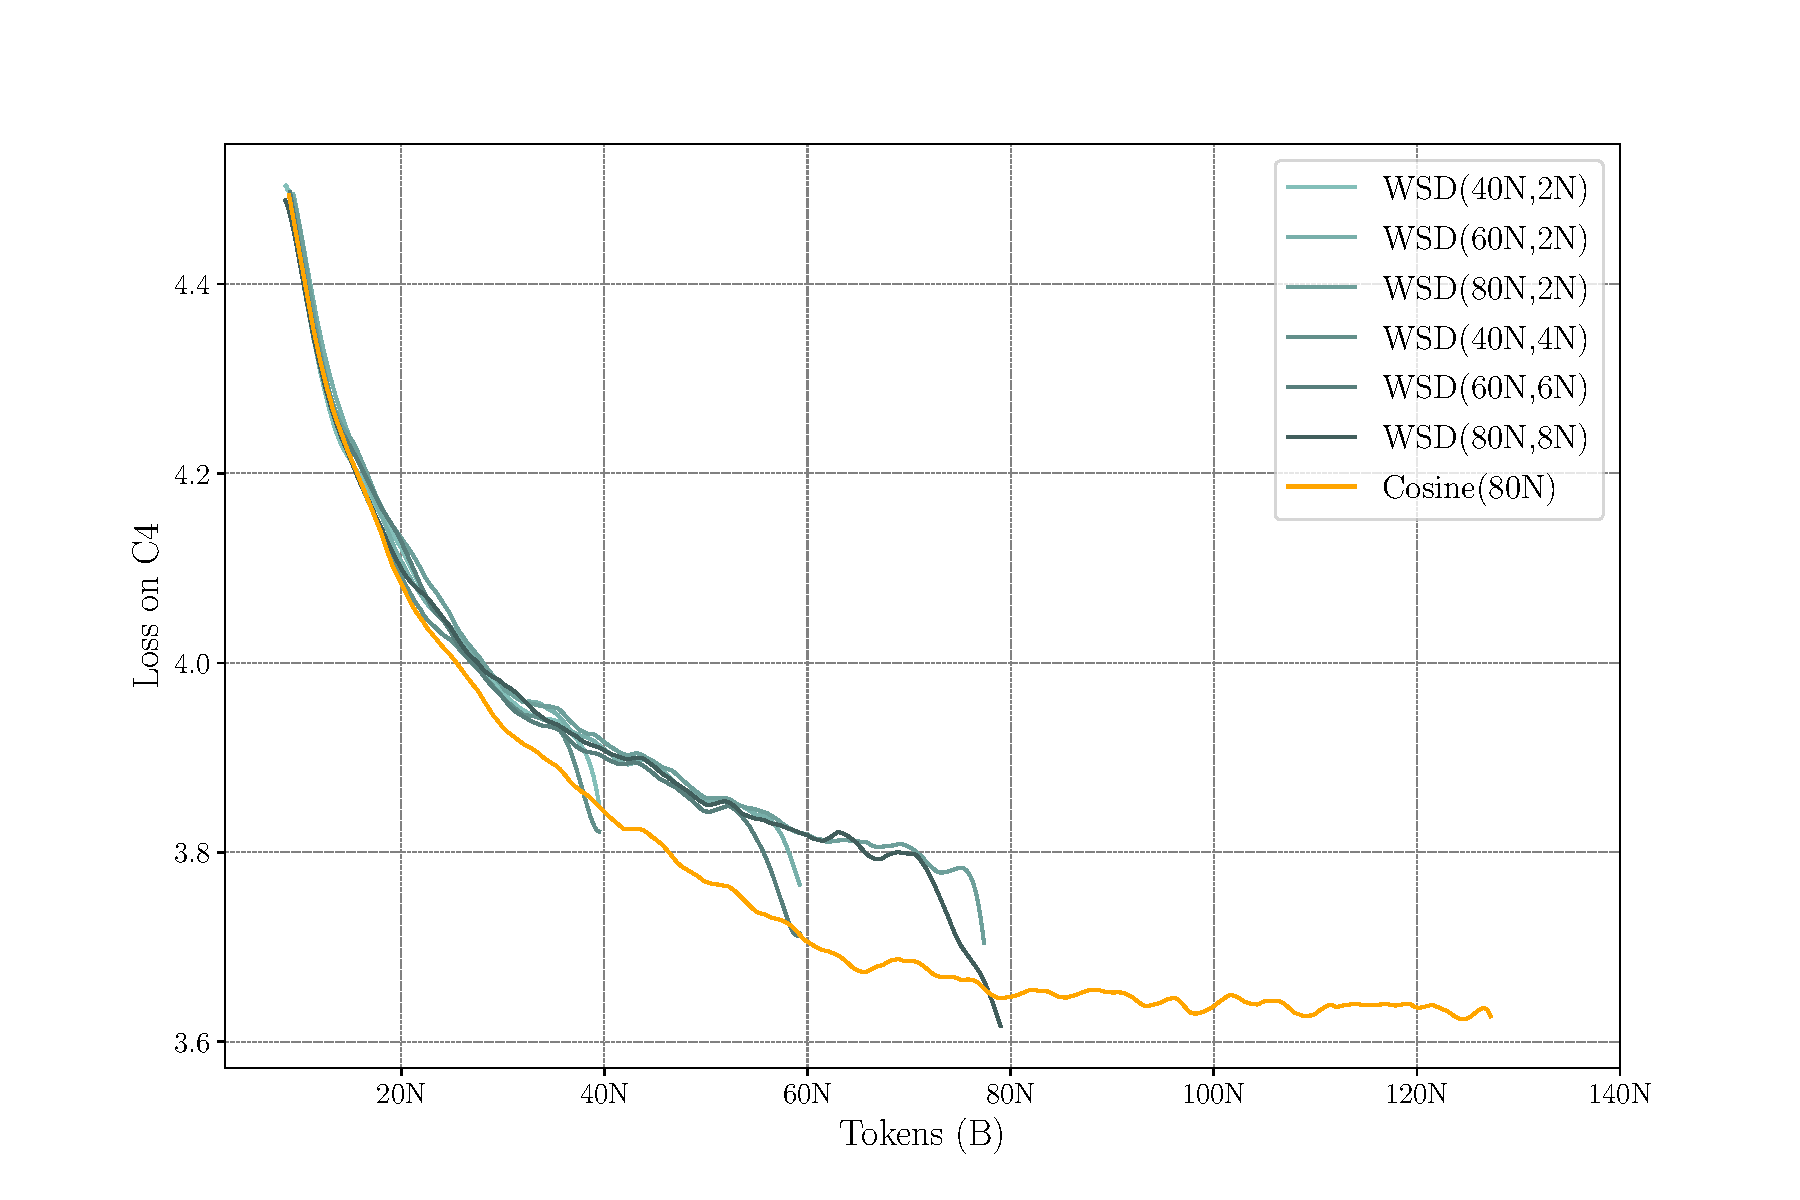
\includegraphics[width=1.05\linewidth]{minicpmFig/WSD_diff_dcay.pdf}
    \caption{ Model training loss has a sudden decrease in the decay stage of WSD LRS. }
    \label{fig:wsd_diff_dcay}
\end{figure}

\begin{figure}[htbp]
    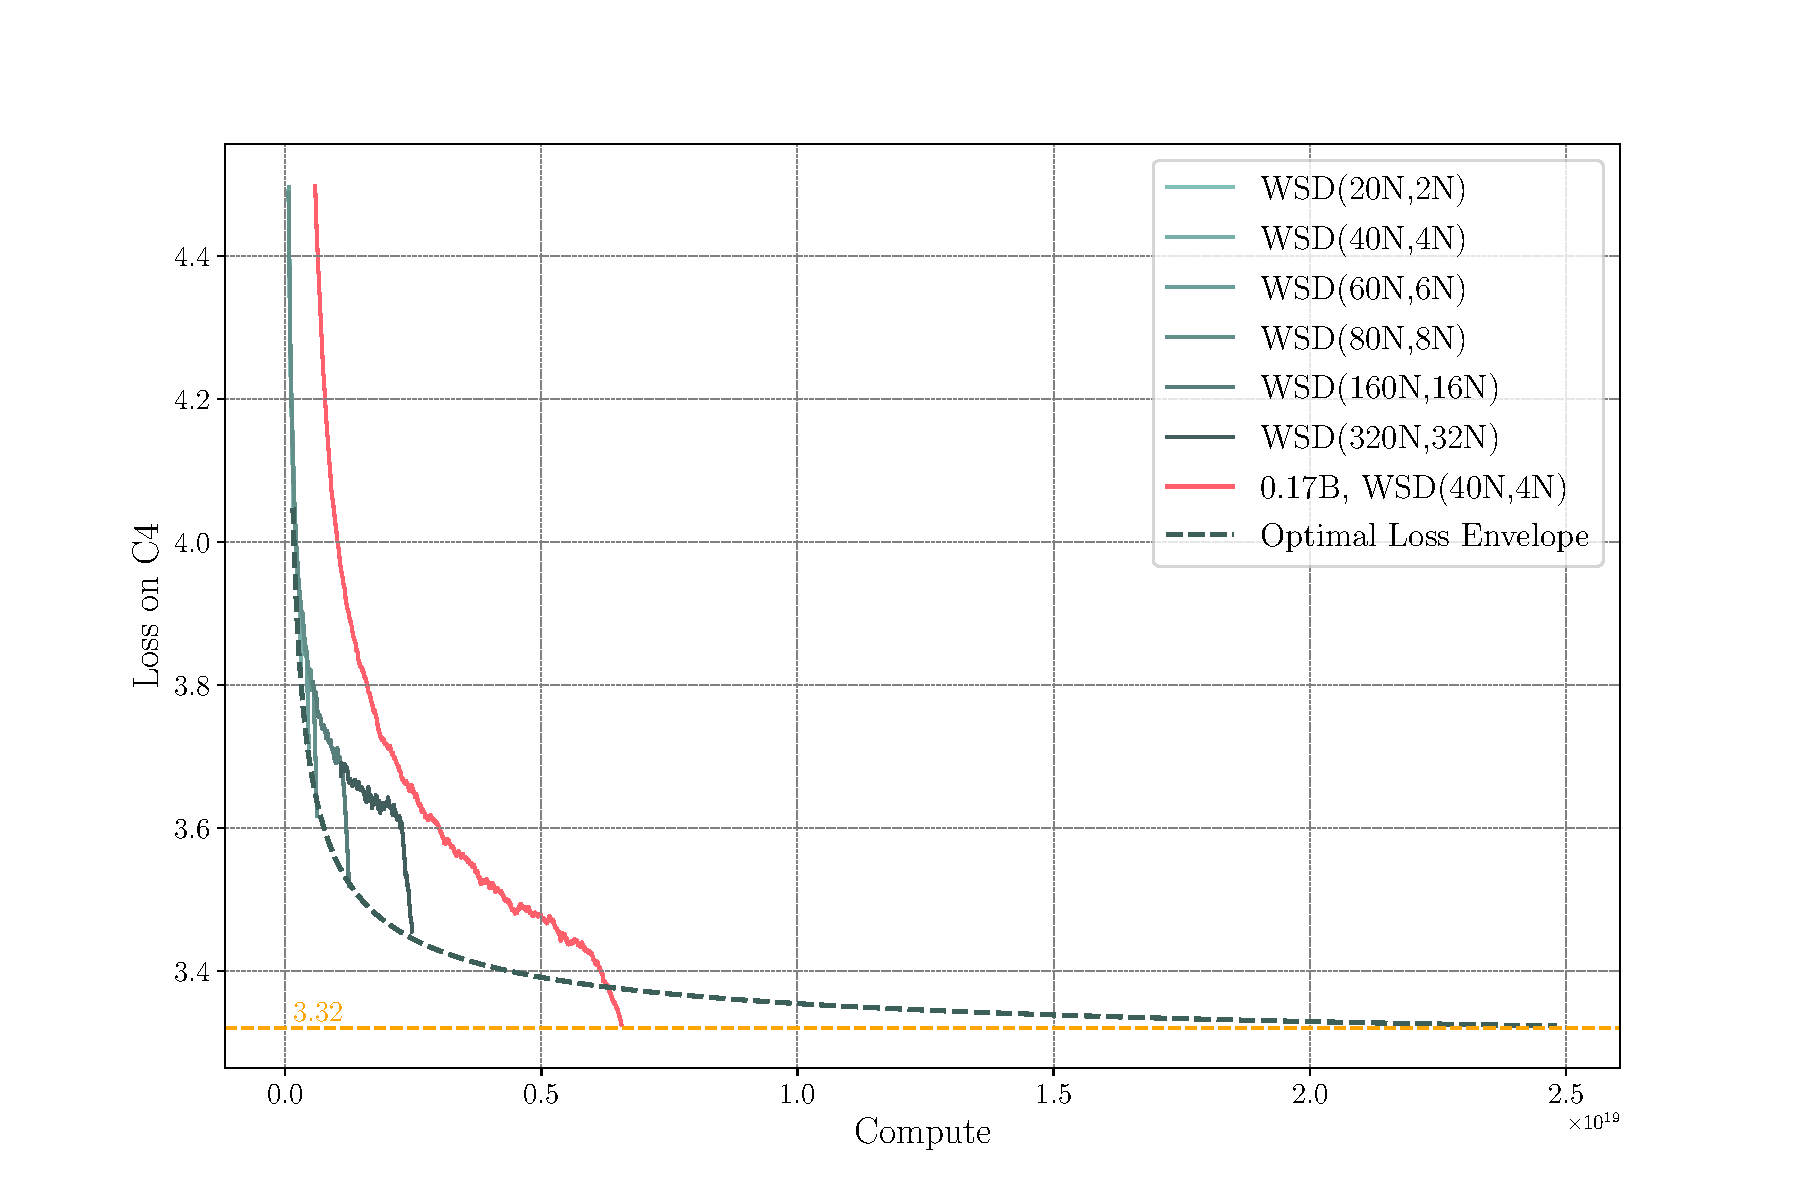
\includegraphics[width=1.05\linewidth]{minicpmFig/continuous_train.pdf}
    \caption{Continous training a 0.036B model can match the performance of 0.17B model with an acceptable increase in training compute.}
    \label{fig:continuoustrain}
\end{figure}


\section{实验}
\label{sec:wsd_experiments_continoustrain}
接下来,我们展示WSD学习率调度器(WSD LRS)的几个实验结果。

\textbf{衰减阶段损失急剧下降。} 我们在0.036B参数规模的模型上尝试WSD LRS。如图\ref{fig:wsd_diff_dcay}所示,在衰减阶段,随着学习率开始下降,损失经历显著快速下降,并迅速降至与$T = S$时的余弦退火学习率调度器(Cosine LRS)相等或更低的水平。同时,我们可以重用衰减前的模型,并以之前的高学习率继续训练。经过更多步训练$S'$后,我们也可以进行退火操作,以达到与$Cosine(S')$时的Cosine LRS相同的损失。这验证了我们的假设,即训练阶段可以明确地划分为稳定训练阶段和衰减阶段。

\textbf{10\%的步数就足够。} 从两阶段训练的角度来看,缩短衰减阶段将极大有利于对稳定训练的不同模型检查点进行快速测试。因此,我们进行实验,从相同的稳定训练检查点开始,但具有不同的衰减步数。同样如图\ref{fig:wsd_diff_dcay}所示,在40N、60N和80N训练数据的所有三个稳定训练检查点中,使用总词元数10\%的衰减量就足以获得最佳结果,而使用总词元数2.5\%的衰减量则无法达到。因此,在后续的训练实验中,我们使用约10\%的衰减量以确保充分收敛。

\textbf{WSD LRS下的有效数据缩放。} 使用WSD LRS,我们可以持续训练语言模型(LM)直至极度收敛。为进一步展示将固定规模模型训练至收敛的潜力,我们比较了使用40N数据对0.036B的LM和0.17B模型进行持续训练的情况。
在图\ref{fig:continuoustrain}中,绿线表示使用不同稳定训练词元数训练的0.036B模型。尽管0.036B系列的最后一个点所使用的训练词元数比Chinchilla最优值~\citep{hoffmann2022training}多得多,但它仍有性能提升空间。

\definecolor{darkgreen}{rgb}{0.0, 0.5, 0.0}

为找到对这个固定规模的LM进行持续训练的极限,我们估计在持续训练过程中模型的最优性能如何随其计算量变化。这里的最优性能,是指通过${WSD}(D, 0.1D)$得到的训练词元$D$的损失。对于一系列的$D$,这些损失将形成最优损失包络线。由于不确定损失包络线的函数形式,我们尝试了两个拟合公式:(1) 指数形式:$L(C) = \alpha e^{-\beta C} + L_0$ 以及 (2) 幂律形式:$L(C) = \beta C^{-\alpha} + L_0$。这两个函数的拟合结果展示在图\ref{fig:fit_continue_train}中中。图中的每个点是WSD LRS中衰减阶段的结束点,对应不同的结束步数。我们尝试了两种函数形式:指数形式和多项式形式。拟合结果表明,多项式缩放定律对于持续训练仍是最佳的。 


\begin{figure}[!htbp]
    \centering
    % First minipage for the first figure
        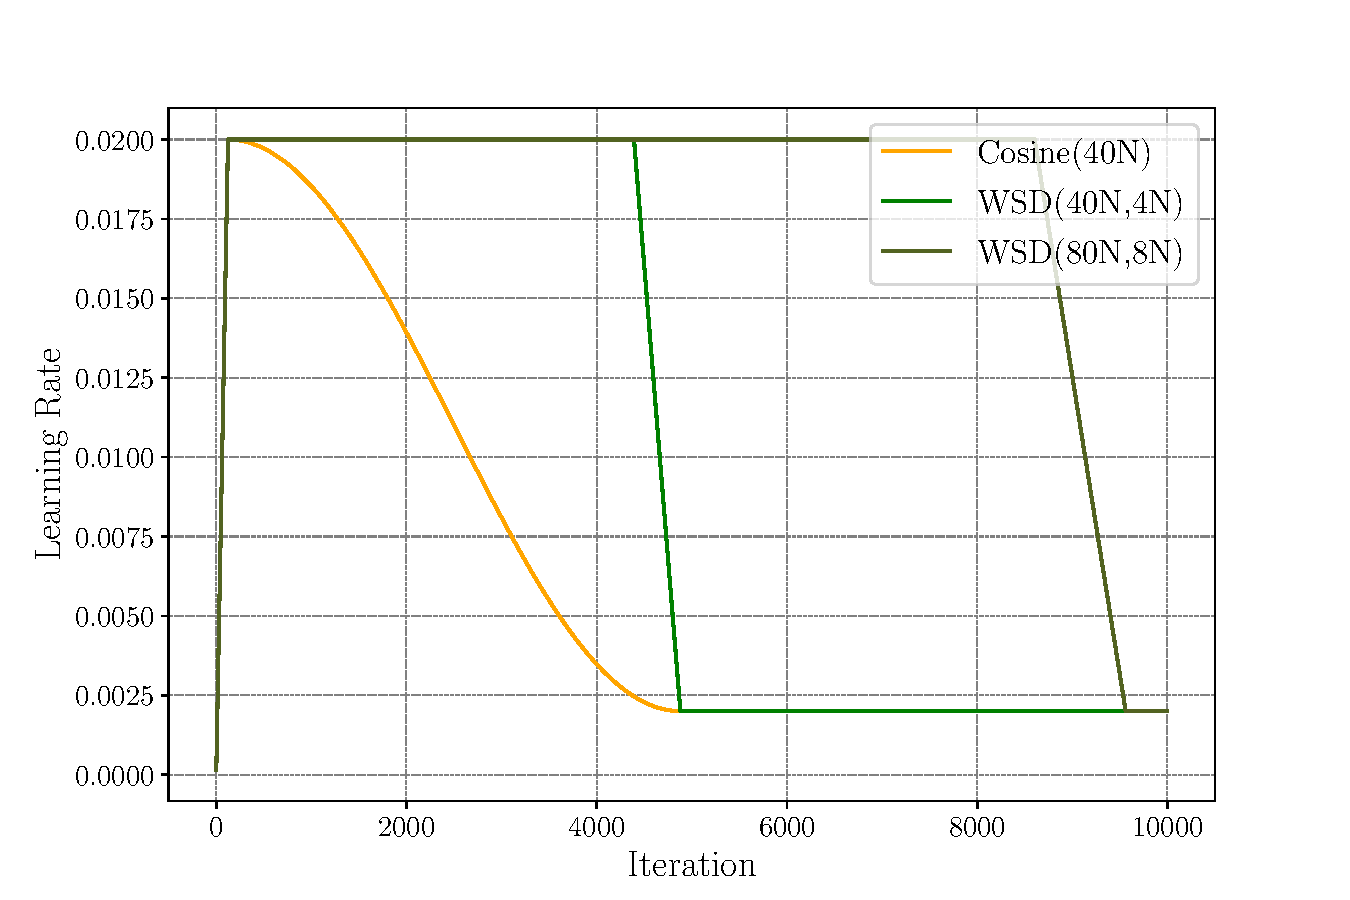
\includegraphics[width=0.98\linewidth]{minicpmFig/lr.pdf}
        \caption{Illustrative comparison between Cosine LRS and WSD LRS. The WSD LRS with different end steps share the same stable training stage. }\label{fig:learning_rate_scheduler_diagram}
\end{figure}
\begin{figure}[!htbp]
    \centering
    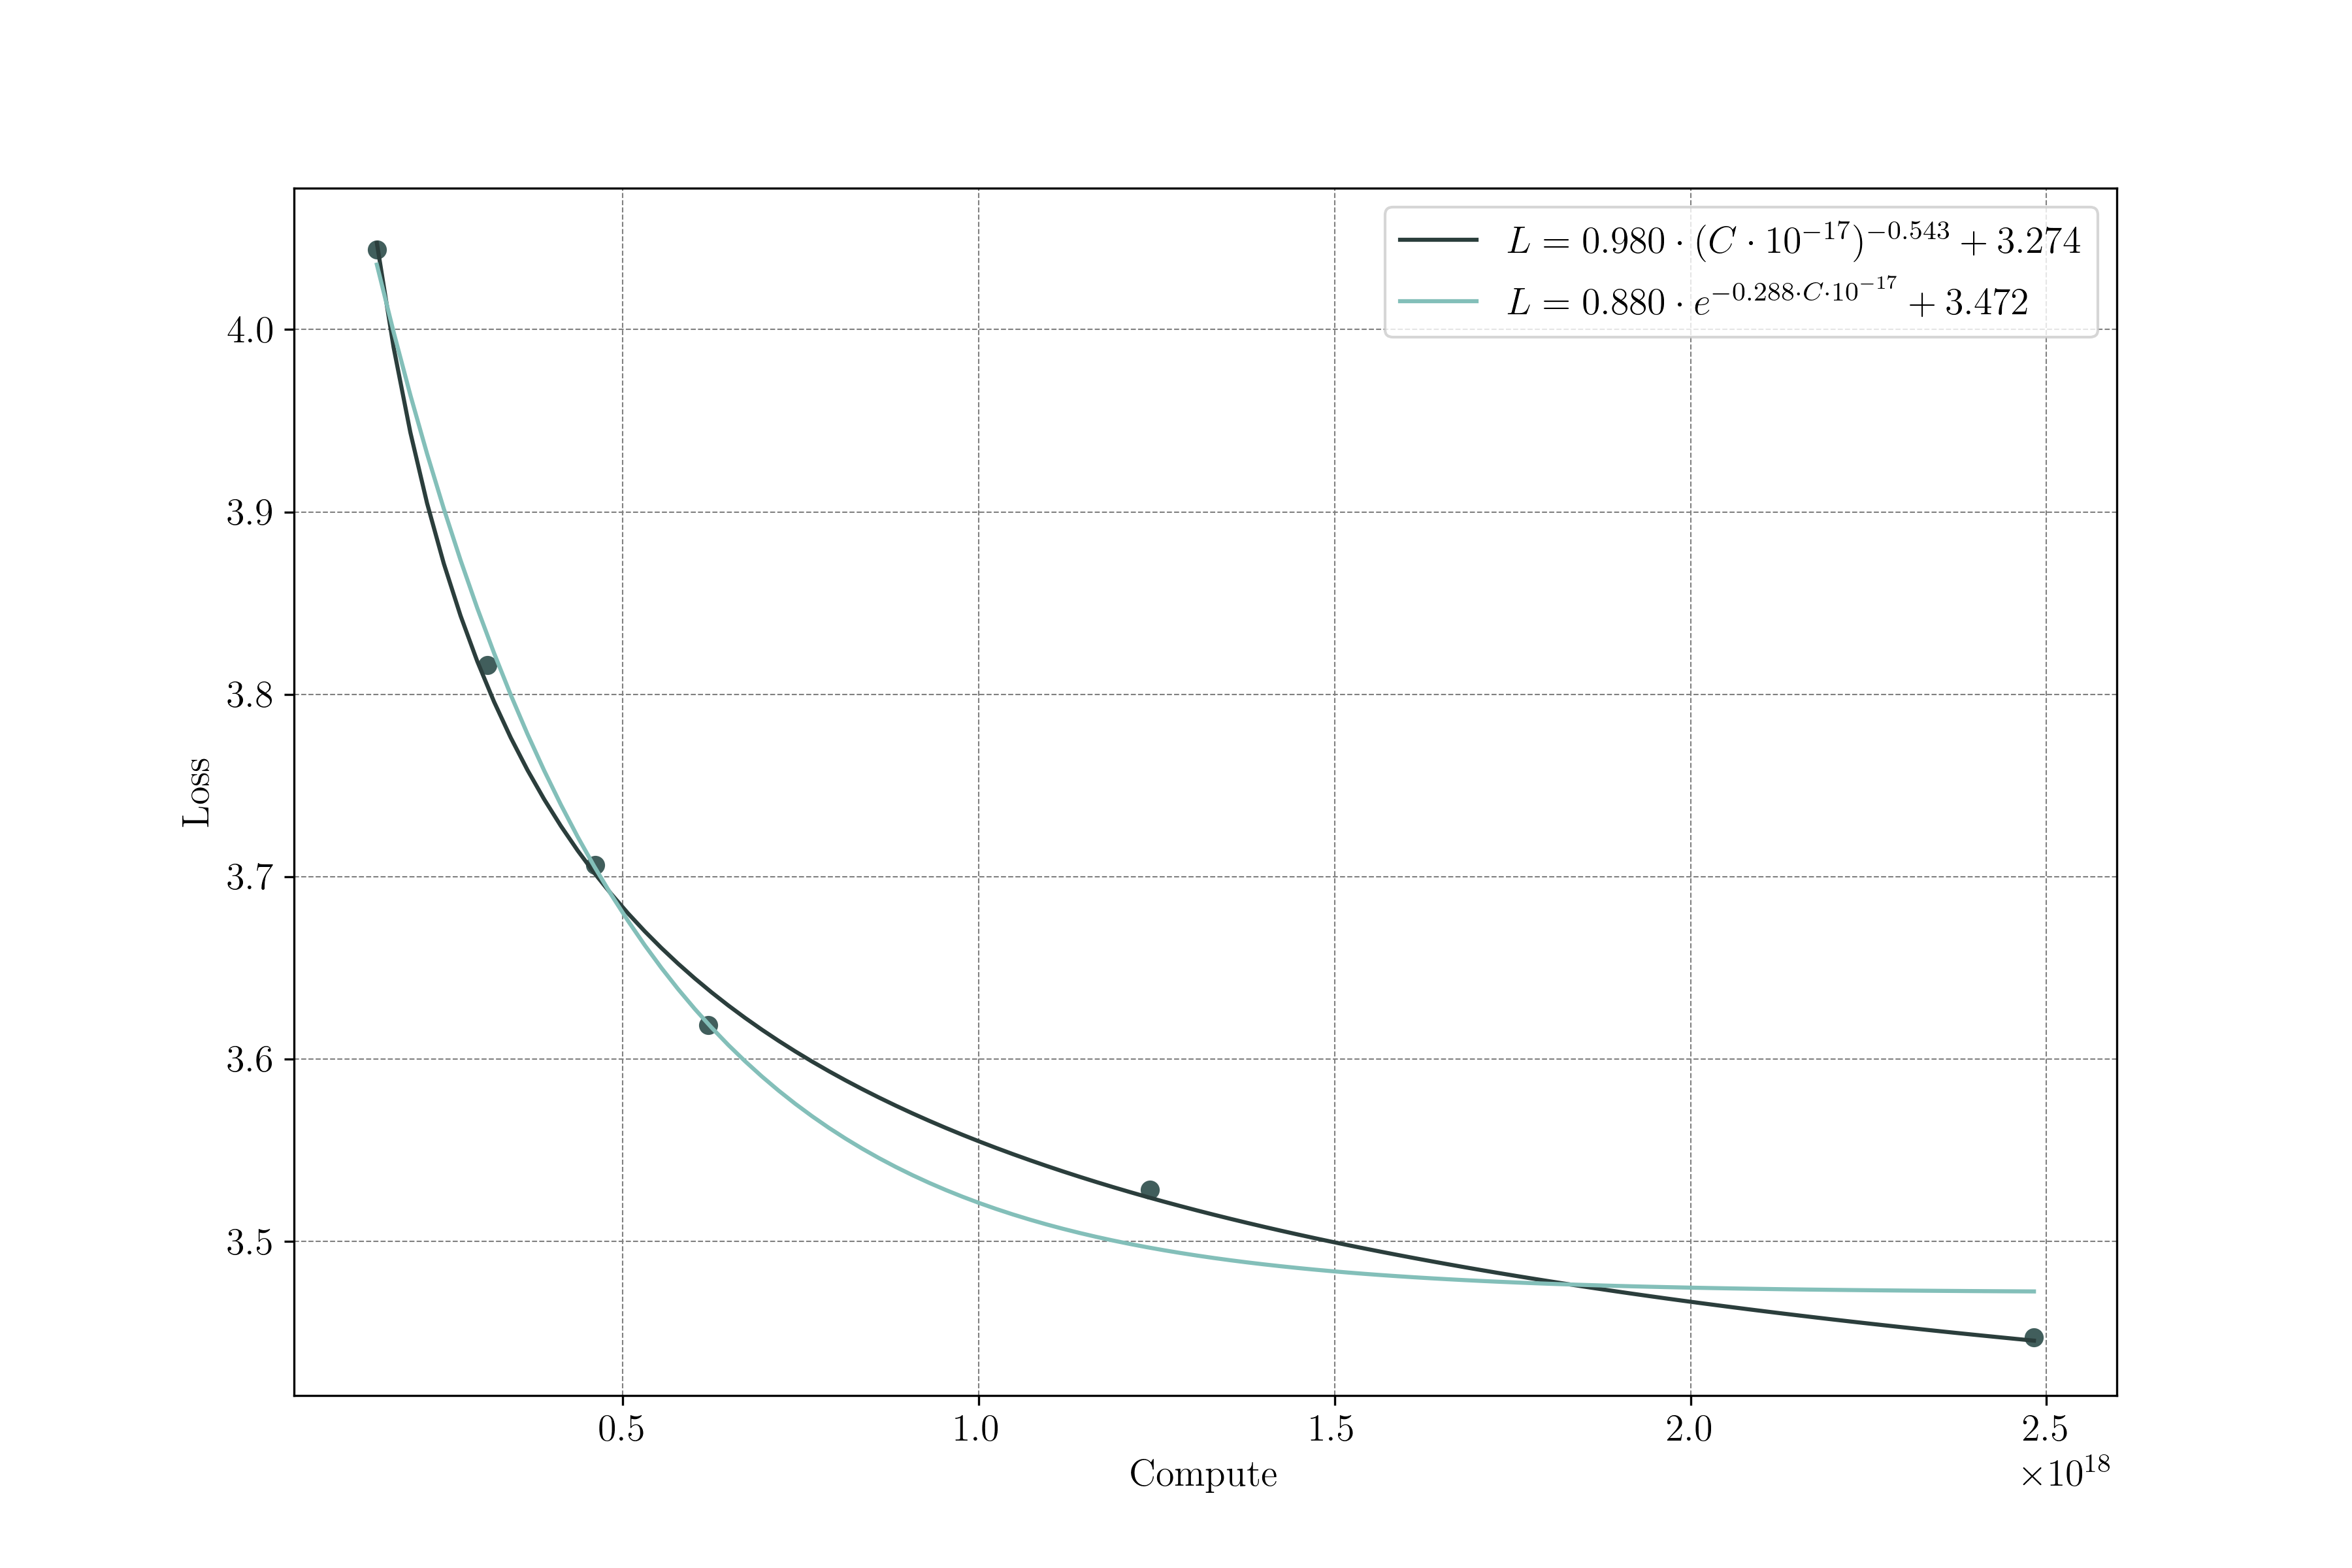
\includegraphics[width=1.05\linewidth]{minicpmFig/fit_continuetrain.png}
    \caption{We use two different function forms to fit the data scaling law achieved by WSD LRS and choose power law as the best fit.}
    \label{fig:fit_continue_train}
\end{figure}



我们发现幂律形式拟合得更好(与Cosine LRS类似~\citep{kaplan2020scaling})。在图\ref{fig:continuoustrain}中,拟合曲线以\textcolor{darkgreen}{绿色}虚线显示。为直观估计和理解对这样一个固定规模模型进行持续训练的效果,我们还使用$WSD(40N, 4N)$训练了一个0.17B模型,在图\ref{fig:continuoustrain}中以\textcolor{pink}{粉色}显示。我们可以看到,一个0.036B模型在训练计算量有可接受的增加(约4倍)的情况下,能够达到与0.17B模型相当的性能,同时节省大量推理计算量~\citep{sardana2023beyond}(每次推理调用节省约5倍),这表明其是一种更好的推理 - 计算最优设置~\citep{sardana2023beyond}。 


\section{衰减阶段分析}
在本节中,我们从检查点更新和梯度信息的角度,对衰减阶段的损失下降进行简要分析。我们计算了MiniCPM - 2.4B(在\ref{sec:model}节中介绍)中所有权重矩阵的最大权重元素更新$max_{ij} (W_{ij}^{(t + 1)} - W_{ij}^{(t)})$。如图\ref{fig:appmaxdiff}所示,这些更新与学习率的大小呈现出很强的相关性。尽管图中展示的是两个子模块(第25层的gate\_proj和q\_proj模块),但这种模式在网络的每一层和子模块中都普遍存在。这一观察结果并非无足轻重:在学习率衰减之前,模型检查点经历了显著更新,但损失减少甚微。相反,在衰减阶段,尽管权重变化不太明显,但损失却加速下降。  

\begin{figure}[t]
    \centering
    % 第一个子图的minipage
        \centering
        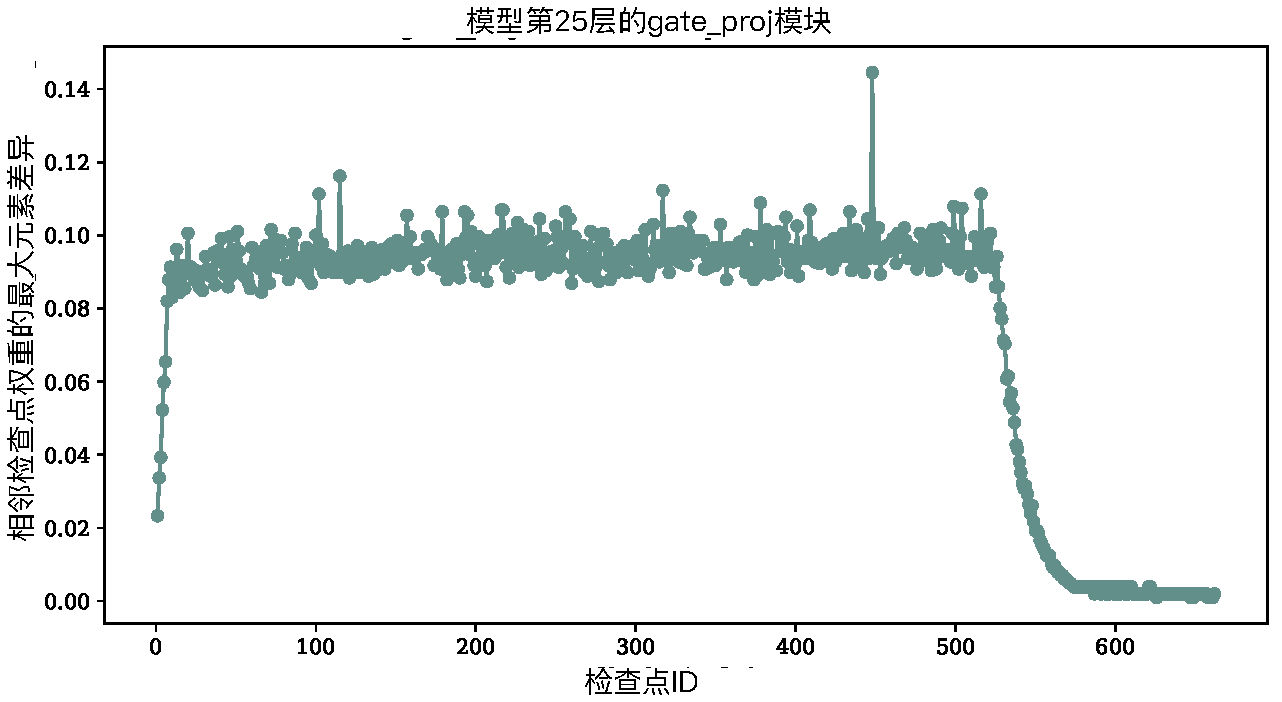
\includegraphics[width=1.0\linewidth]{minicpmFig/gate_proj_projection_vs_rank_25.pdf}
\end{figure}
\begin{figure}[t]
        \centering
        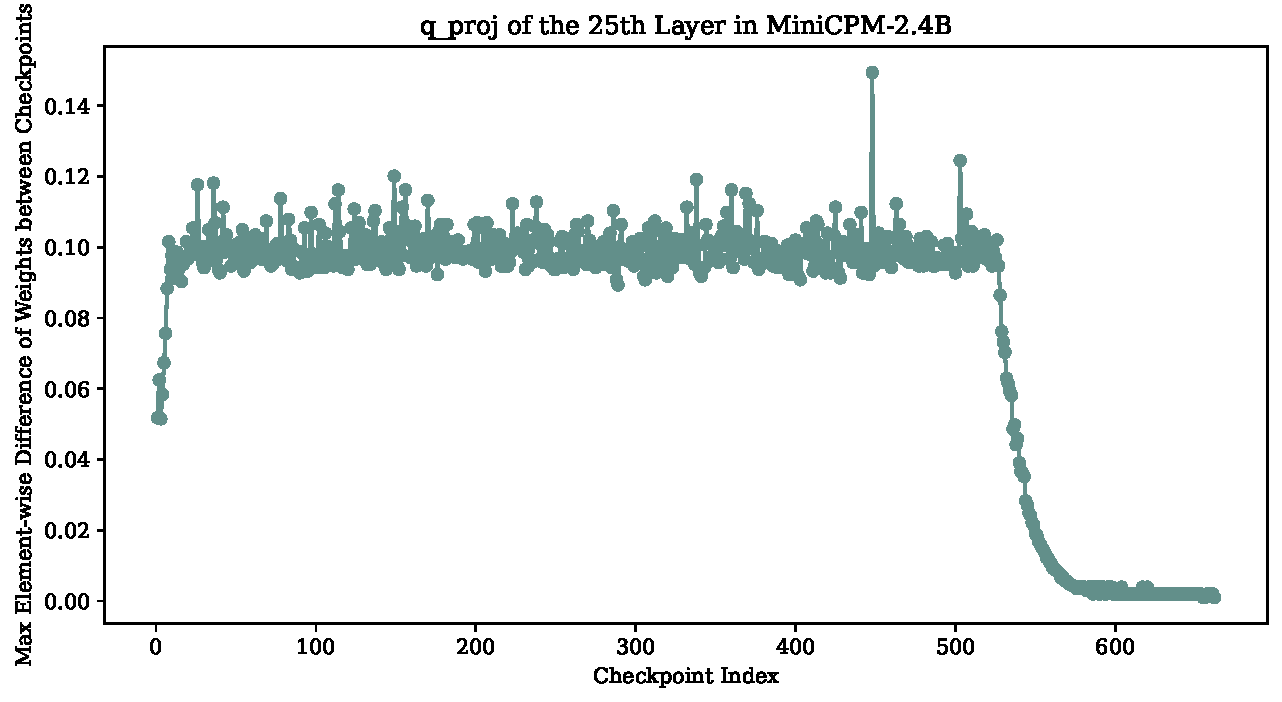
\includegraphics[width=1.0\linewidth]{minicpmFig/q_proj_projection_vs_rank_25.pdf}
     \caption{检查点的最大差异。}
        \label{fig:appmaxdiff}
\end{figure}


\section{使用WSD学习率调度器衡量缩放定律}
\label{scalinglawwsdlrs}
缩放定律是大语言模型(LLMs)发展中的一项基本指导原则。尽管由于不同模型系列的配置各异,这些缩放定律在具体系数上存在差异,但计算最优数据与模型的比率在不同的缩放定律函数中仍是一个有意义的指标,它 “忽略” 了损失的具体数值。关于这一比率,\cite{kaplan2020scaling} 认为模型规模增加十倍应等同于数据规模增加一倍。相反,\cite{hoffmann2022training} 主张模型大小与数据大小的缩放率相同。此外,当前的模型如LLama 2~\citep{touvron2023llama},所使用的训练数据比 \cite{hoffmann2022training} 所宣称的要多得多,却仍能带来显著的性能提升,这表明其数据与模型的比率更高。 

这种尚未解决的不确定性源于传统缩放实验中训练多个不同大小模型和数据规模所固有的挑战。此前,如果在一种数据规模上训练一种模型规模的平均成本为 $C$,那么使用 $m$ 种模型规模和 $m$ 种数据规模进行缩放实验大约需要 $O(m^2)C$ 的成本。 

在本节中,我们介绍使用WSD调度器作为一种有效的方法,以线性成本($O(mC)$)来探索缩放定律。由于WSD调度器具有从任意步数的稳定阶段检查点衰减后达到余弦退火学习率调度器(Cosine LRS)最优损失的优势,我们现在能够精确测量最优缩放属性,而无需将模型从头开始训练到不同数量的词元,从而使沿数据轴的缩放定律测量效率大大提高。

我们通过训练6种规模从0.04B到2B的小语言模型(SLMs)来沿数据轴和模型轴测量缩放定律,每种模型在稳定训练阶段都有6个从 $10N$ 到 $60N$ 数据的检查点开始衰减的模型($N$ 为相应的模型规模)。最终损失在五个留出的评估数据集上进行评估。为了在模型使用不同分词器时能够比较损失,我们按照~\cite{achiam2023gpt},以字节数而非词元数来取损失的平均值。每对数据规模和模型规模的最终损失如图\ref{fig:individual_task_datascalinglaw}中的蓝线所示。 

然后,我们按照 ~\cite{hoffmann2022training} 使用scipy的\texttt{curvefit}函数,用模型规模 $N$ 和数据规模 $D$ 对损失进行拟合:

\begin{equation}
    L(N, D) = C_NN^{-\alpha} + C_DD^{-\beta} + L_0
\label{equ:scalinglaw}
\end{equation}

每个数据集和每个检查点沿数据轴的拟合曲线如图\ref{fig:individual_task_datascalinglaw}中的橙线所示。然后,在给定固定计算量 $C = 6ND$~\citep{rae2021scaling} 的情况下,我们得到最优模型规模 $N_{opt}$ 和数据集规模 $D_{opt}$ 为: 
\begin{figure}
    \centering
    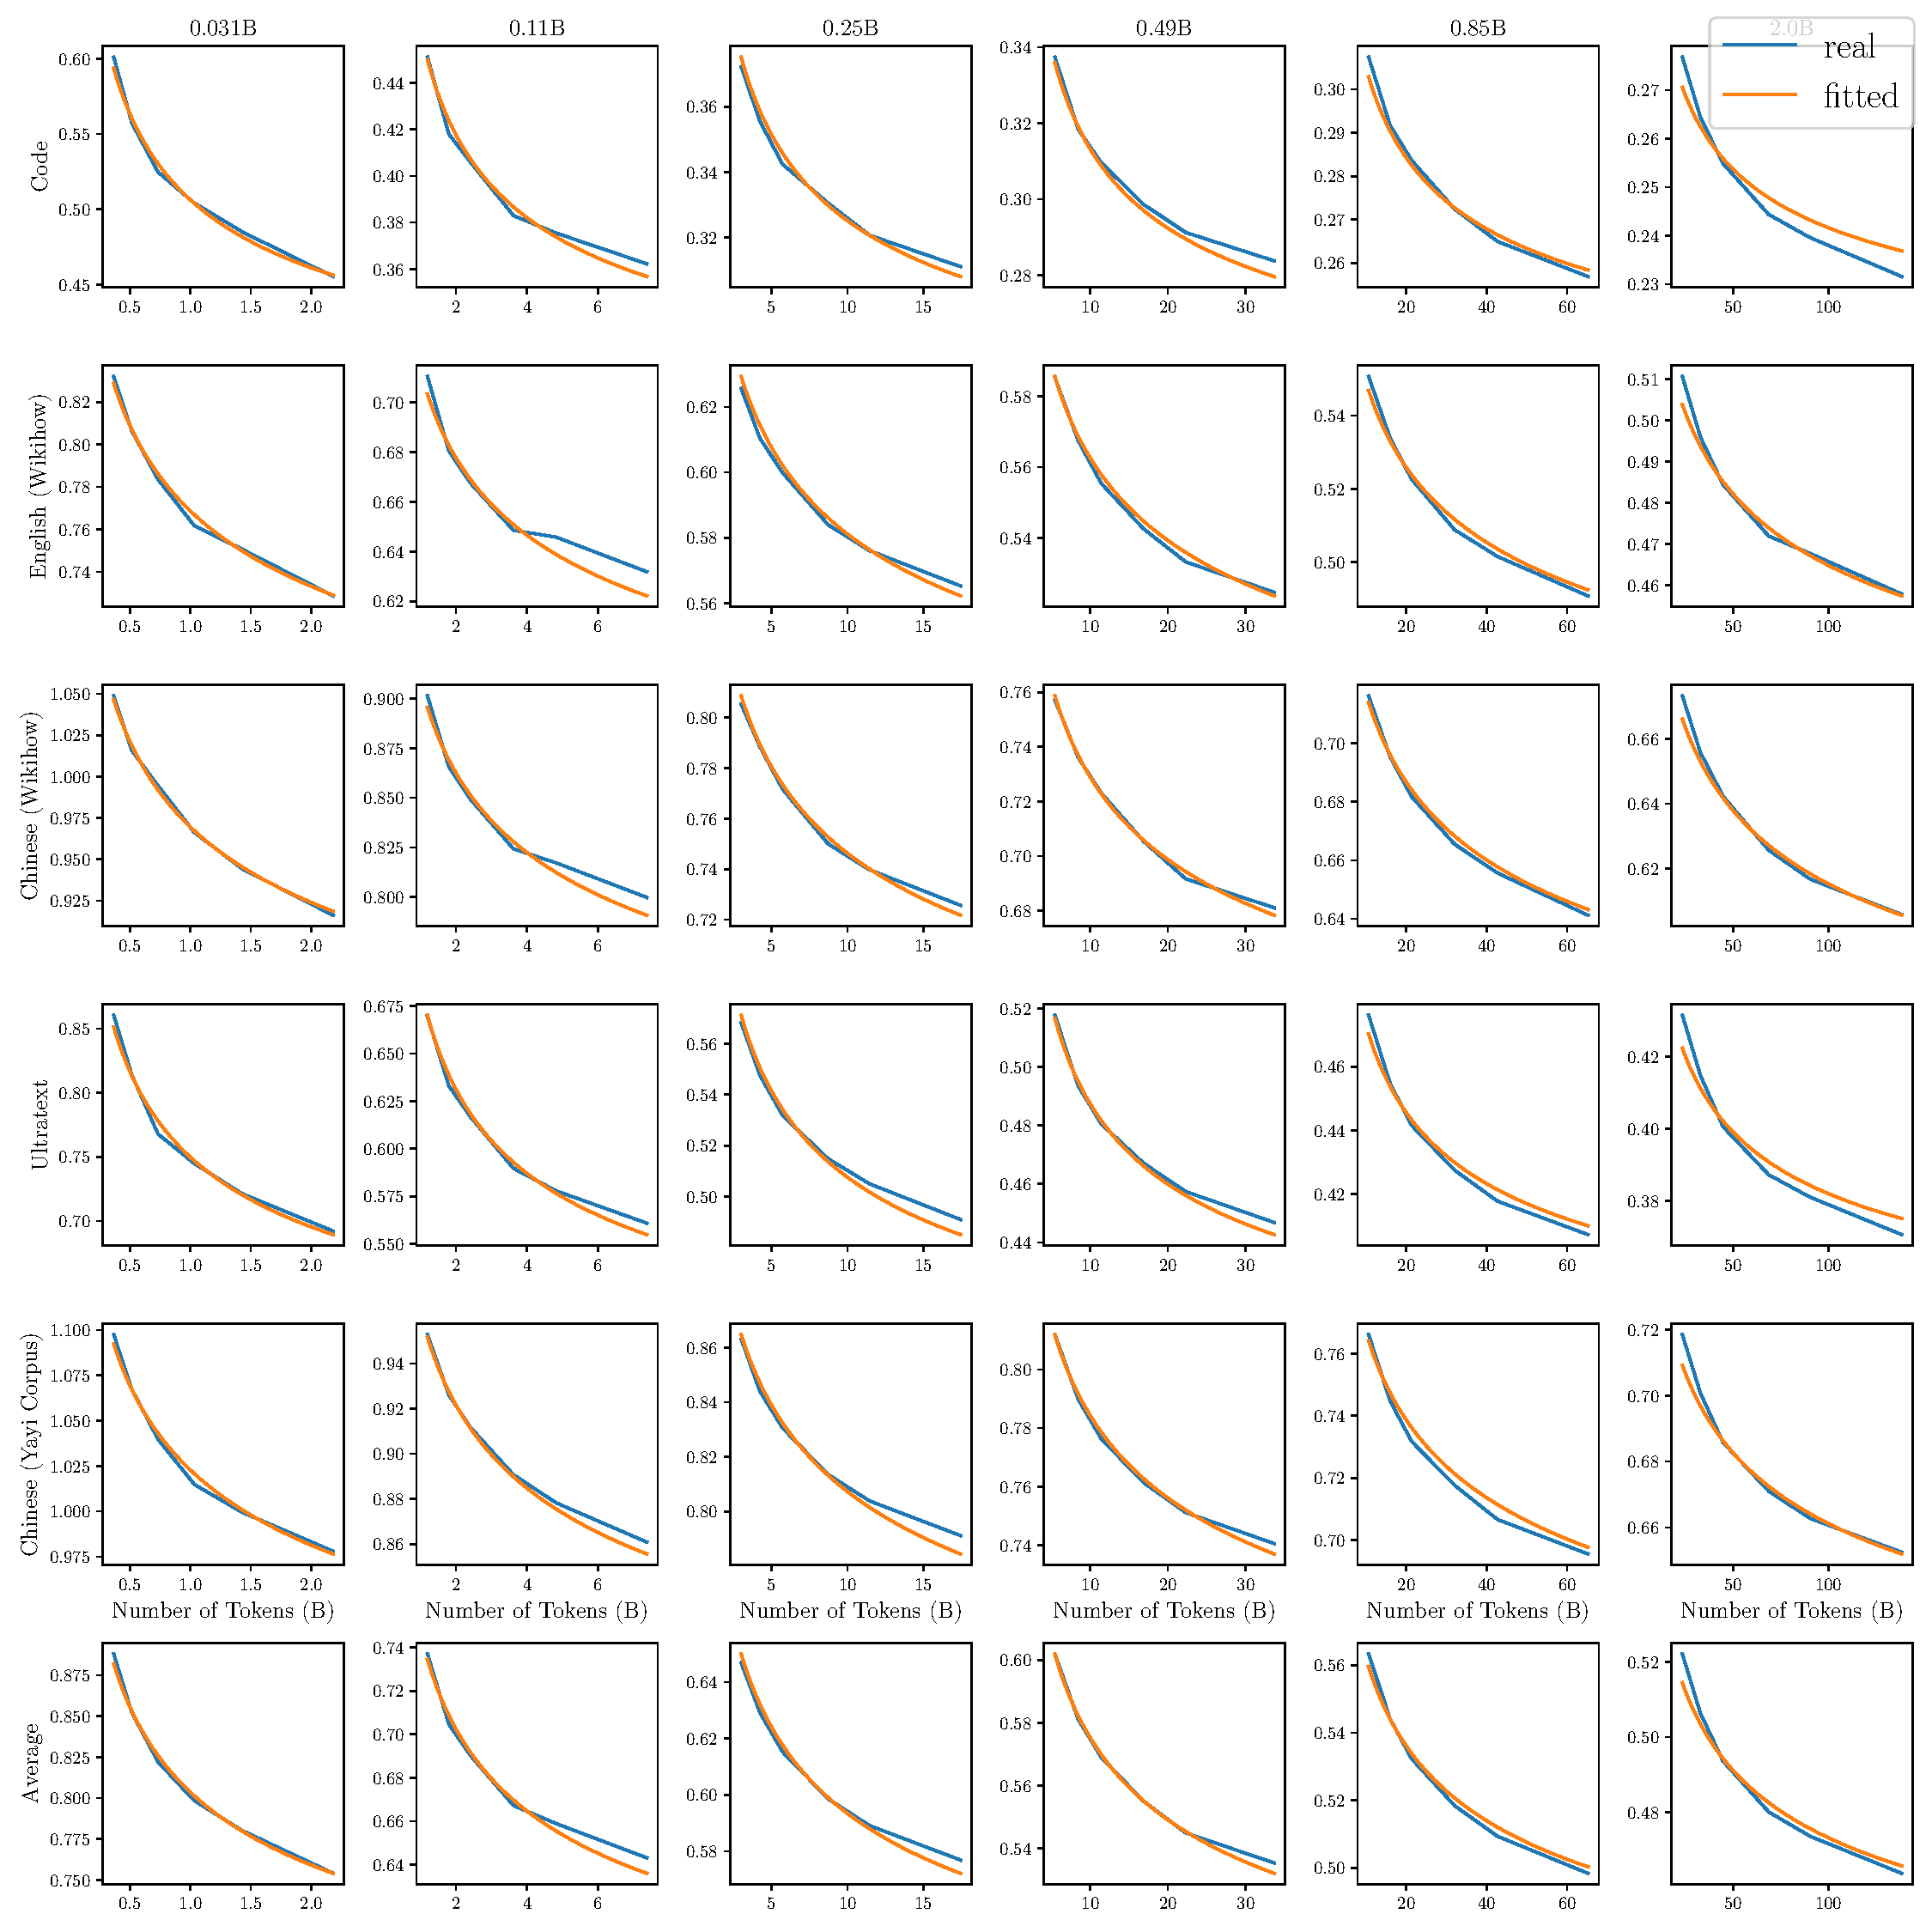
\includegraphics[width=1.0\textwidth]{minicpmFig/individual_task_datascalinglaw.pdf}
    \caption{针对每个模型和每个任务,沿数据量轴绘制的拟合缩放定律。除了0.11B和0.25B模型的最后检查点外,拟合结果令人满意。}
    \label{fig:individual_task_datascalinglaw}
\end{figure}


\begin{equation}
    \frac{N_{opt}}{D_{opt}} = K^2\left(\frac{C}{6}\right)^{\eta},
\label{equ:computeoptimal}
\end{equation}

其中 $K = (\frac{\alpha C_N}{\beta C_D})^{\frac{1}{\alpha + \beta}} $,且 $\eta=\frac{\beta - \alpha}{\alpha + \beta}$。$N_{opt}$ 的推导紧密遵循 ~\cite{hoffmann2022training},将公式\ref{equ:scalinglaw} 中的 $D$ 替换为 $\frac{C}{6N}$,并在给定 $C$ 的情况下最小化 $L(N)$。$D_{opt}$ 的推导采用类似方法。 
从公式\ref{equ:computeoptimal} 可知,当 $\alpha = \beta$ 时,$N_{opt}/D_{opt}$ 为常数,支持了 ~\cite{hoffmann2022training} 的观点;当 $\alpha < \beta$ 时,我们应更强调参数缩放~\citep{kaplan2020scaling},反之亦然。 

在我们的实验中,损失与 $N$、$D$ 之间的拟合关系如图\ref{fig:wsd_optimalscalinglaw} 中损失等值线图所示。每个子图中第一个文本框显示拟合缩放定律的方程。我们可以看到,在所有评估语料库中,$\beta < \alpha$。更具体地说,平均而言,$\alpha = 0.29$,$\beta = 0.23$,$K^2 = 0.01$,$\eta = -0.10$(注意 $N$ 在 $10^9$ 以下,$D$ 在 $10^9$ 以下,$C$ 在 $10^{18}$ 以下)。由于 $\alpha$ 略大于 $\beta$,这一结果表明,随着计算规模的变化,我们应比模型缩放更略微强调数据缩放,这与 ~\cite{hoffmann2022training} 的观点一致。

至于具体的数据与模型的比率 $\frac{D_{opt}}{N_{opt}}$,我们注意到,尽管我们的结果与 ~\cite{hoffmann2022training} 中 $\frac{D_{opt}}{N_{opt}}$ 随计算量 $C$ 变化的趋势一致,但在计算最优区域仍存在巨大差距。具体而言,平均数据规模应比模型规模大192倍,而 ~\cite{hoffmann2022training} 中为20倍。我们注意到这与\ref{sec:wsd_experiments_continoustrain} 节和图\ref{fig:continuoustrain} 中的观察结果一致。

关于与Chinchilla最优的 $\frac{N_{opt}}{D_{opt}}$ 存在较大偏差,我们注意到他们的缩放实验是在一个不是非常新的配置下进行的。为了与更新的配置(如Llama2~\citep{touvron2023llama})进行比较,我们从Llama2论文中提取训练损失数据(附录图\ref{fig:llamascaling} 的左半部分),并使用图\ref{fig:llamascaling} 的右半部分估计他们论文中的计算最优 $\frac{D_{opt}}{N_{opt}}$。由于他们使用的是Cosine LRS,在训练中间阶段损失并非最优,如图\ref{fig:llamascaling} 右图中训练期间的凹曲线所示。我们用一条直线填充凹形部分,以估计如果他们使用WSD LRS时的最优损失包络线。在此之后,计算模型规模大致应是一个模型的损失曲线即将与更大模型的损失曲线相交的区域。基于此直觉,13B模型在 $10^5$ EFlops($10^{18}$ Flops)时即将与34B模型相交,34B模型在 $5\times 10^5$ EFlops 时即将与70B模型相交。因此,我们估计 $\frac{D_{opt}}{N_{opt}}$ 大致为 $\frac{5\times 10^5}{6\times 34^2} \sim \frac{10^5}{6\times 13^2} $,即 $70 \sim 100$。因此,在这种近似比较下,他们的数据与模型比率更接近我们的结果。与之前的配置相比,我们的配置可以将更多数据融入较小的模型中。然而,我们注意到上述估计只是一个粗略的结果。 

更大的数据与模型比率意味着我们可以比之前认为的将更多数据融入较小的模型中,这对于推理和部署来说效率更高。我们希望WSD LRS将帮助更多研究人员以更少的精力探索 $L(N, D)$,并使大语言模型中的这种关系更加清晰。 


\begin{figure}[!t]
    \centering
    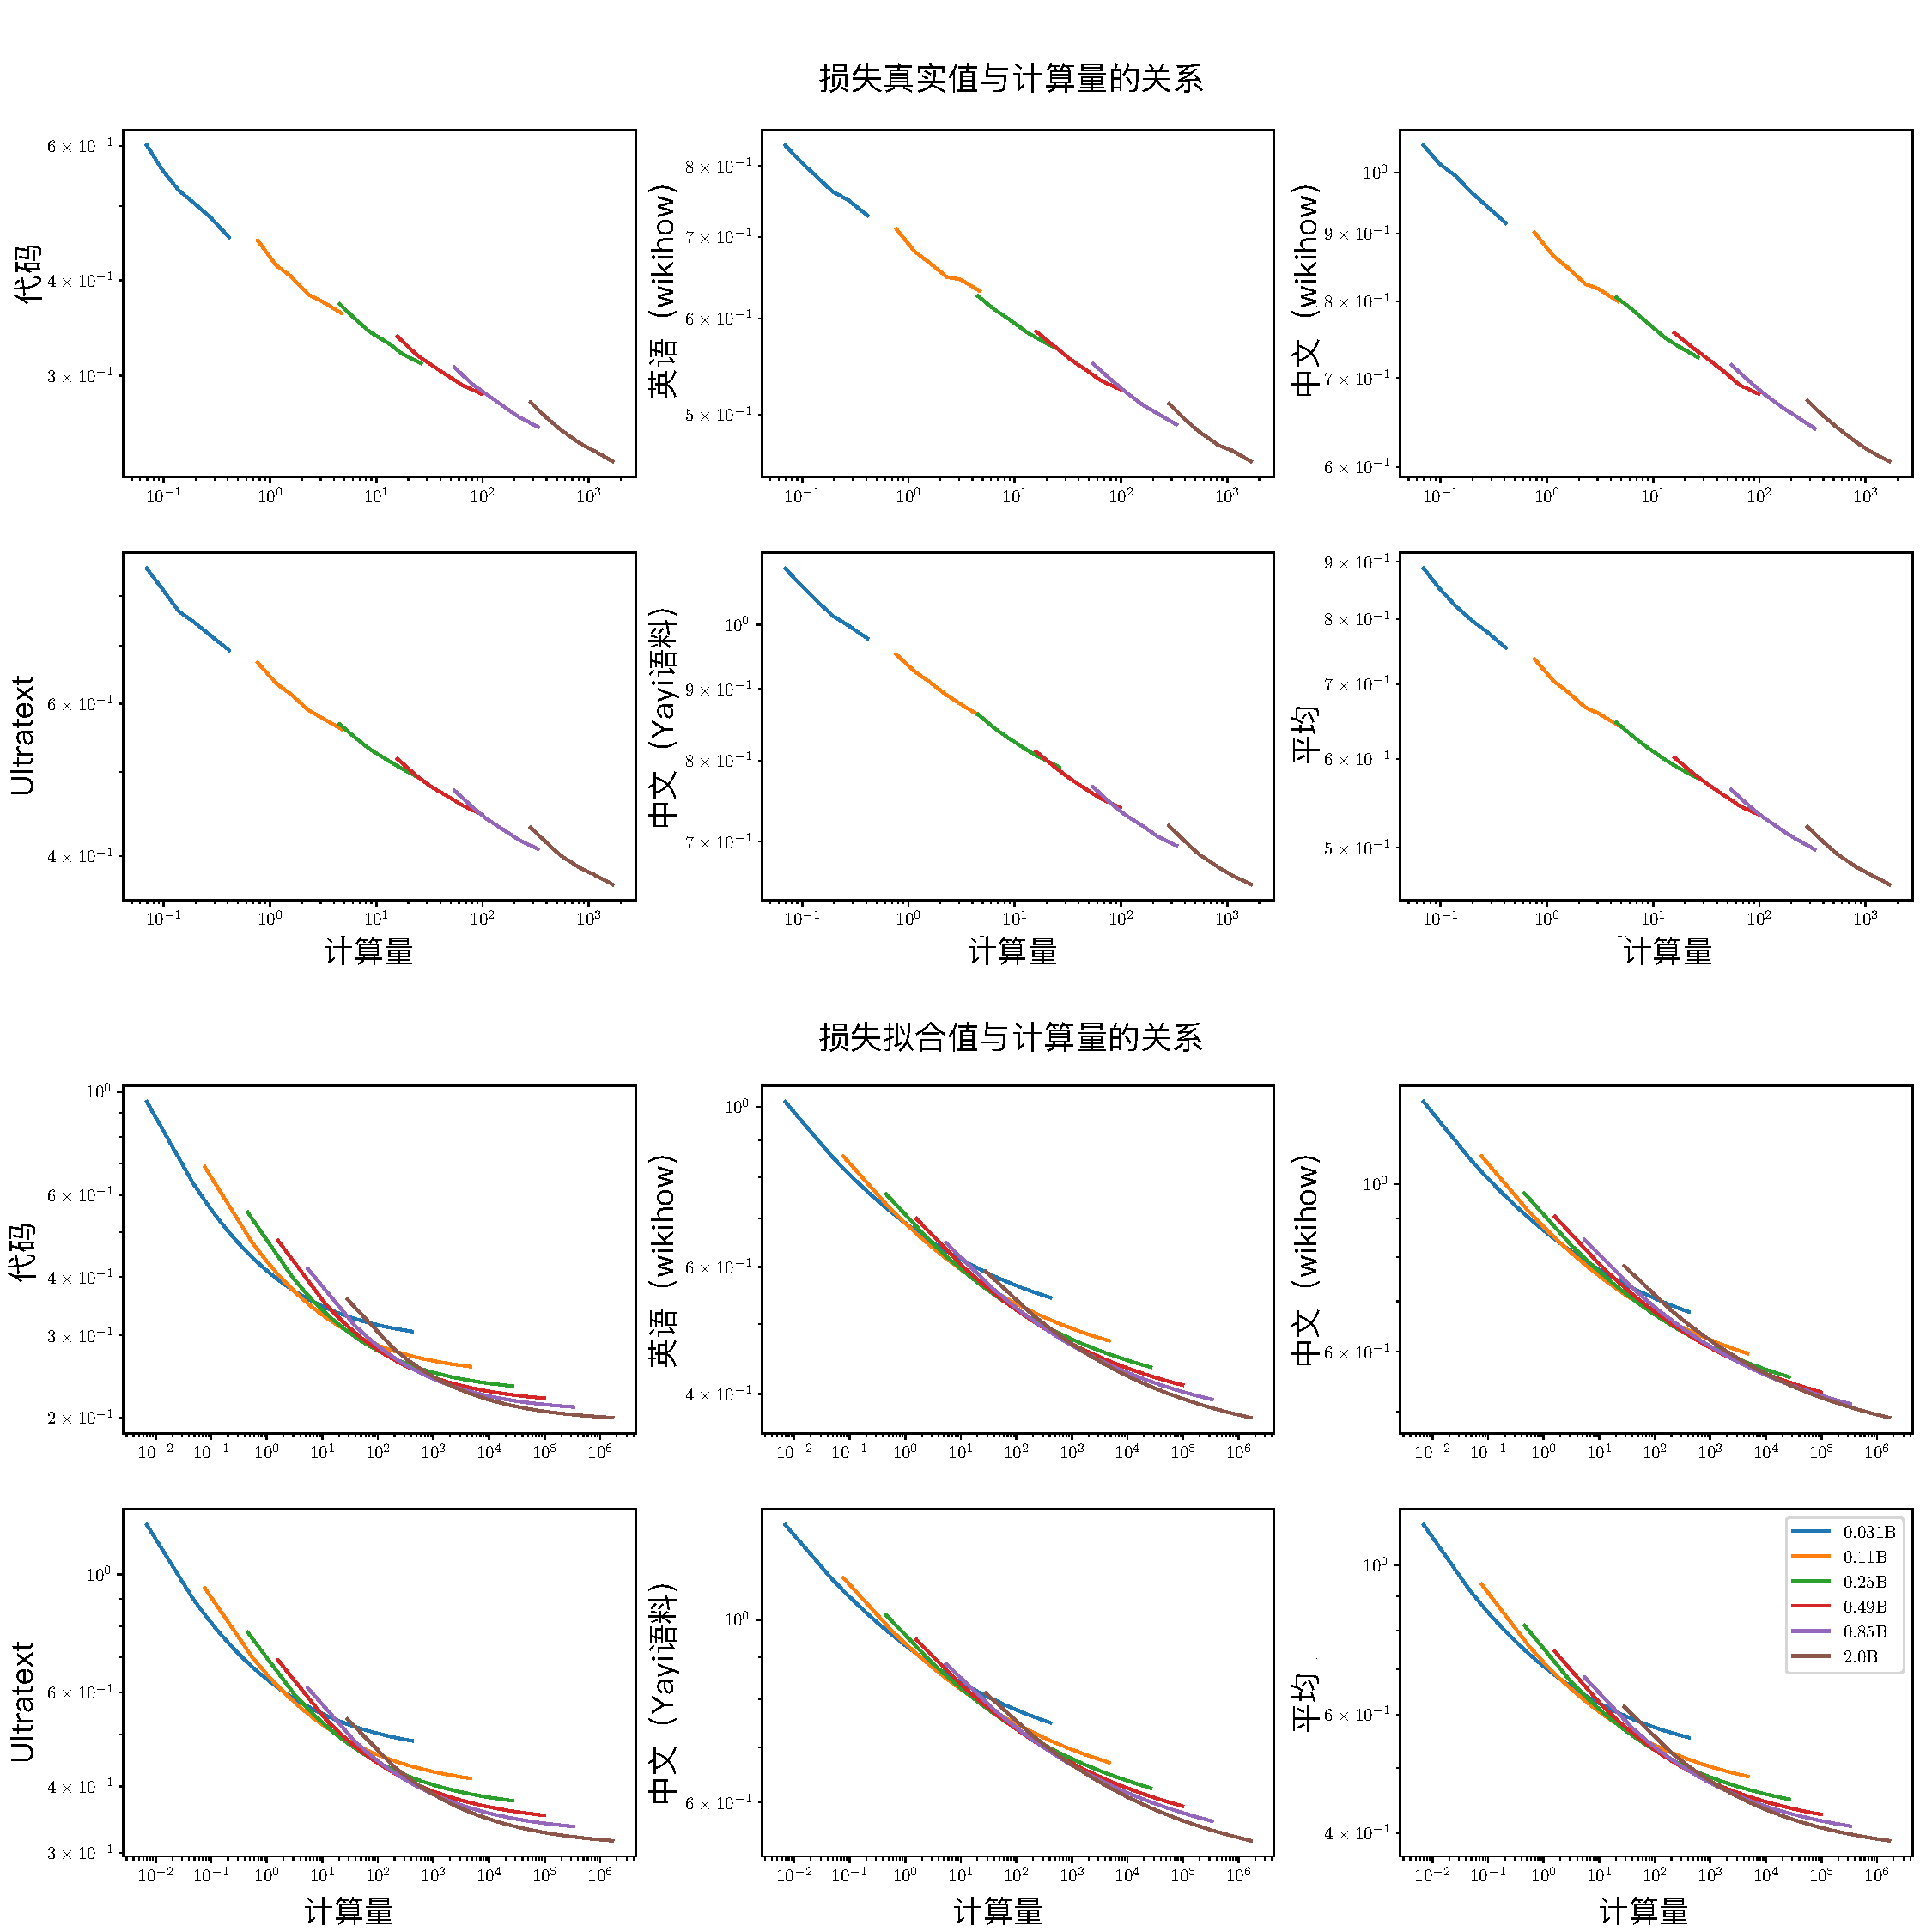
\includegraphics[width=\textwidth]{minicpmFig/lossvscompute_fitted_and_real.pdf}
    \caption{使用WSD调度器进行缩放实验的结果(上图)以及拟合的缩放曲线(下图)。x轴为计算量Flops,$C = 6ND$,每条线的颜色代表相同模型但具有不同的计算量Flops。我们可以看到,当Flops较小时,较小的模型表现优于较大的模型;而当Flops较大时,较小的模型表现较差。因此,不同规模的模型在图中计算最优区域附近会相互交叉。}
    \label{fig:wsd_optimalscalinglaw}
\end{figure}

\begin{figure}[!t]
    \centering
    \includegraphics[width=1.0\textwidth]{minicpmFig/wsd_optimal_scaling_law.pdf}
    \caption{使用WSD调度器进行缩放实验的拟合结果。水平线上的黑点表示相同模型规模下不同计算量中的衰减检查点。图例中的$C$为语义完整以Flops为单位表示,未使用EFlops单位。y轴上的$C$以EFlops为单位。}
    \label{fig:wsd_optimalscalinglaw}
\end{figure}



\section{Llama2数据与模型比率的分析}
如\ref{scalinglawwsdlrs}节所述,我们基于Llama2的训练损失曲线分析其数据与模型比率。提取的损失绘制在图\ref{fig:llamascaling}的左侧。我们将x轴转换为计算量Flops,以便在图的右侧比较计算最优区域。

\begin{figure}
    \centering
    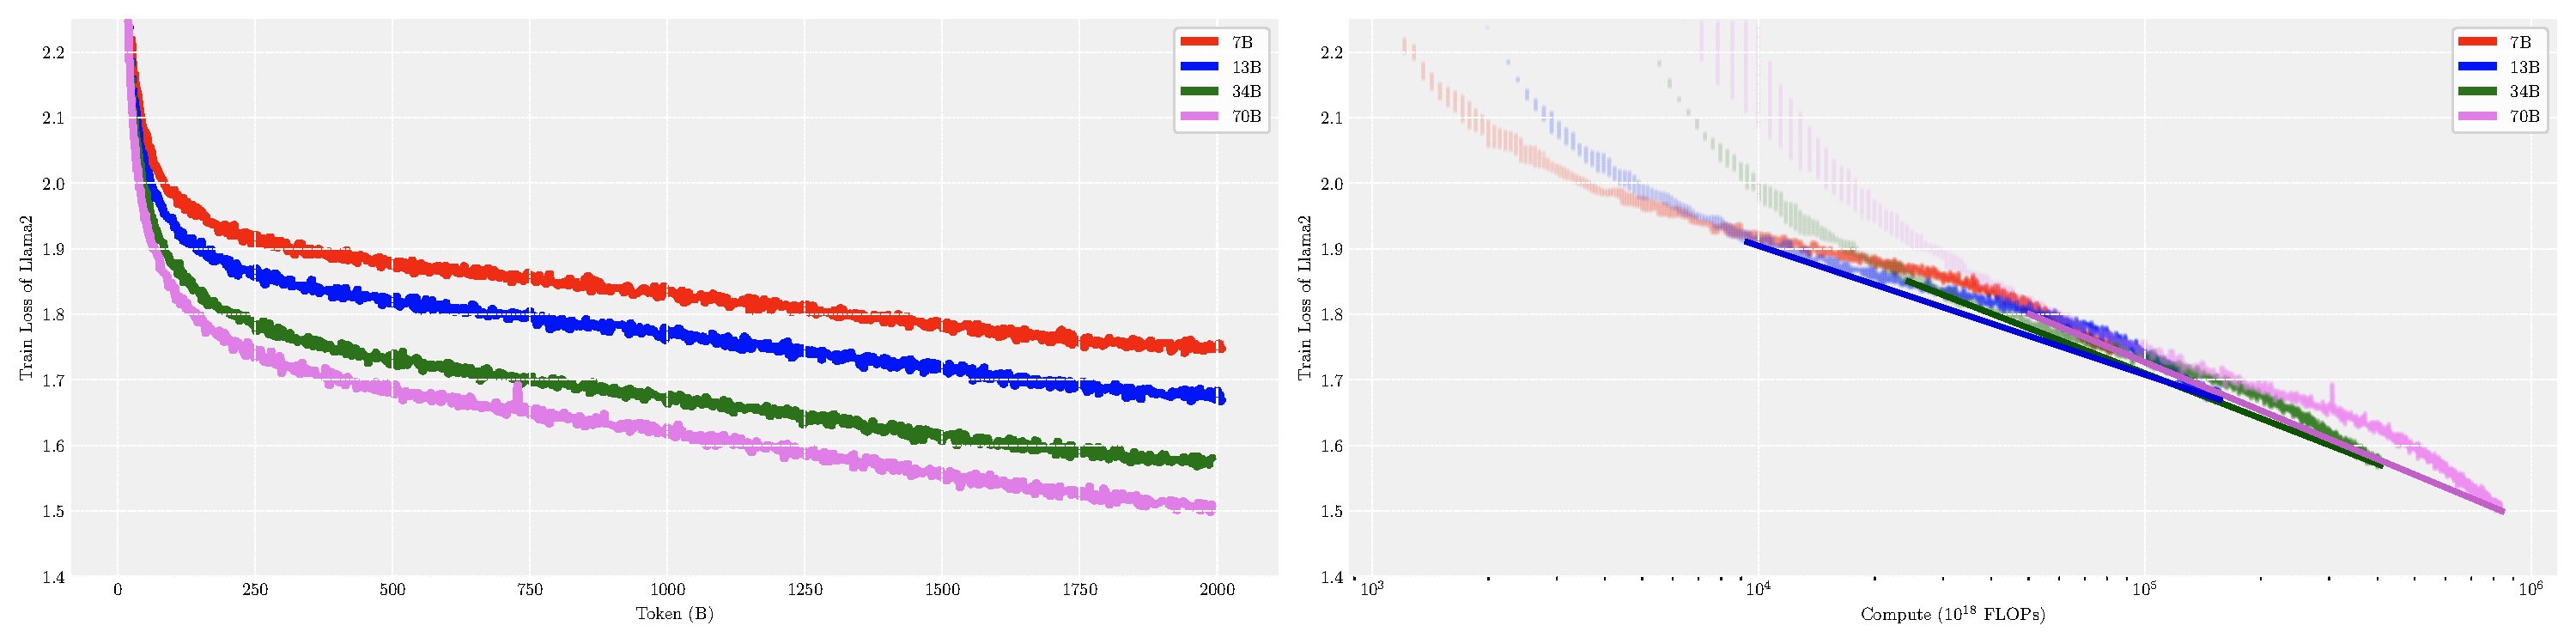
\includegraphics[width=1.0\textwidth]{minicpmFig/llama2_scaling.pdf}
    \caption{我们从Llama2论文中提取训练损失数据(左图部分),并使用右图部分估计其论文中的计算最优$\frac{D_{opt}}{N_{opt}}$。绘制的直线是假设使用WSD调度器来估计最优损失包络线。}
    \label{fig:llamascaling}
\end{figure}

% !TeX root = ../thuthesis-example.tex



\chapter{可预测预训练--性能可预测训练}

前面介绍了可预测预训练的训练策略部分。在使用包括超参数可预测扩展、基于新型学习率调度的可预测扩展的预训练方案之后,本文已经可以准确地预测不同模型规模和数据规模下的训练损失。然而即便如此,对于可预测预训练的目标而言,这也仅给出了不完整的答案。优化损失的确会随着模型规模的增加而按预期下降,这与大家熟知的大模型扩展定律相符;但学术界尚未建立关于下游任务性能(后简称性能或任务)的扩展定律。实际上,在模型规模的扩展过程中,性能远非可预测的。性能通常在小模型上提升较小,直到模型超过某个规模阈值后才会显著提升,这就是所谓 “涌现能力” 的典型表现。在本章中,我将深入研究这一现象,力图在”性能涌现“的背景下,建立起性能的平滑扩展定律。具体而言,我发现小模型尽管性能提升幅度较小,但展现出关键且持续的任务性能改进,由于测量分辨率不足,传统评估策略未能捕捉到这些改进。为了衡量这种改进,本章引入了 “PassUntil”评估策略,这是一种在解码阶段通过大量采样实现理论上无限分辨率的评估策略。借助 “PassUntil”,我对任务性能的扩展定律进行了定量研究。该研究包含两个部分。首先,我确定了一种严格的 “任务扩展定律”,这超过了学术届对于任务性能不可预测的认知。本文能够在训练开始前预测24亿参数模型在代码生成任务上的性能,偏差仅为0.05\%。其次,基于 “PassUntil”,本文对涌现能力进行了定量研究。我识别出一种 “加速涌现”,其扩展曲线无法用标准扩展定律函数拟合,且增长速度不断加快。然后我检验了两个假设,并暗示 “多回路假设” 可能是导致加速涌现的原因。 本章将详细介绍基于 “PassUntil”方法的性能可预测预训练。

\section{背景}
\subsection{损失连续性与性能突变性的矛盾}

大语言模型令人瞩目的成功在很大程度上依赖于扩大模型参数和预训练数据量。一直以来的观察表明,当考虑一系列架构近乎相同的模型时,更大的模型规模以及更多的预训练语料库总能使训练损失降低。这一观察结果已在数学上被形式化为损失扩展定律 \citep{kaplan2020scaling, henighan2020scaling}。该定律指出,模型在对数尺度下可降低的损失(L)与对数尺度下的模型规模(N)呈线性关系。扩展定律为大语言模型的科学扩展提供了指导,包括确定模型规模与预训练数据规模的平衡 \citep{hoffmann2022training, muennighoff2023scaling}。这将曾经略显盲目的扩展过程转变为一种有实证依据的方法。

然而,这种有益的扩展定律仅对损失做出预测,并未延伸到实际中遇到的真实任务性能。这种差异在全面的规模化方法中造成了巨大的差距 \citep{ganguli2022predictability}。

\begin{figure}[!htbp]
        \centering
        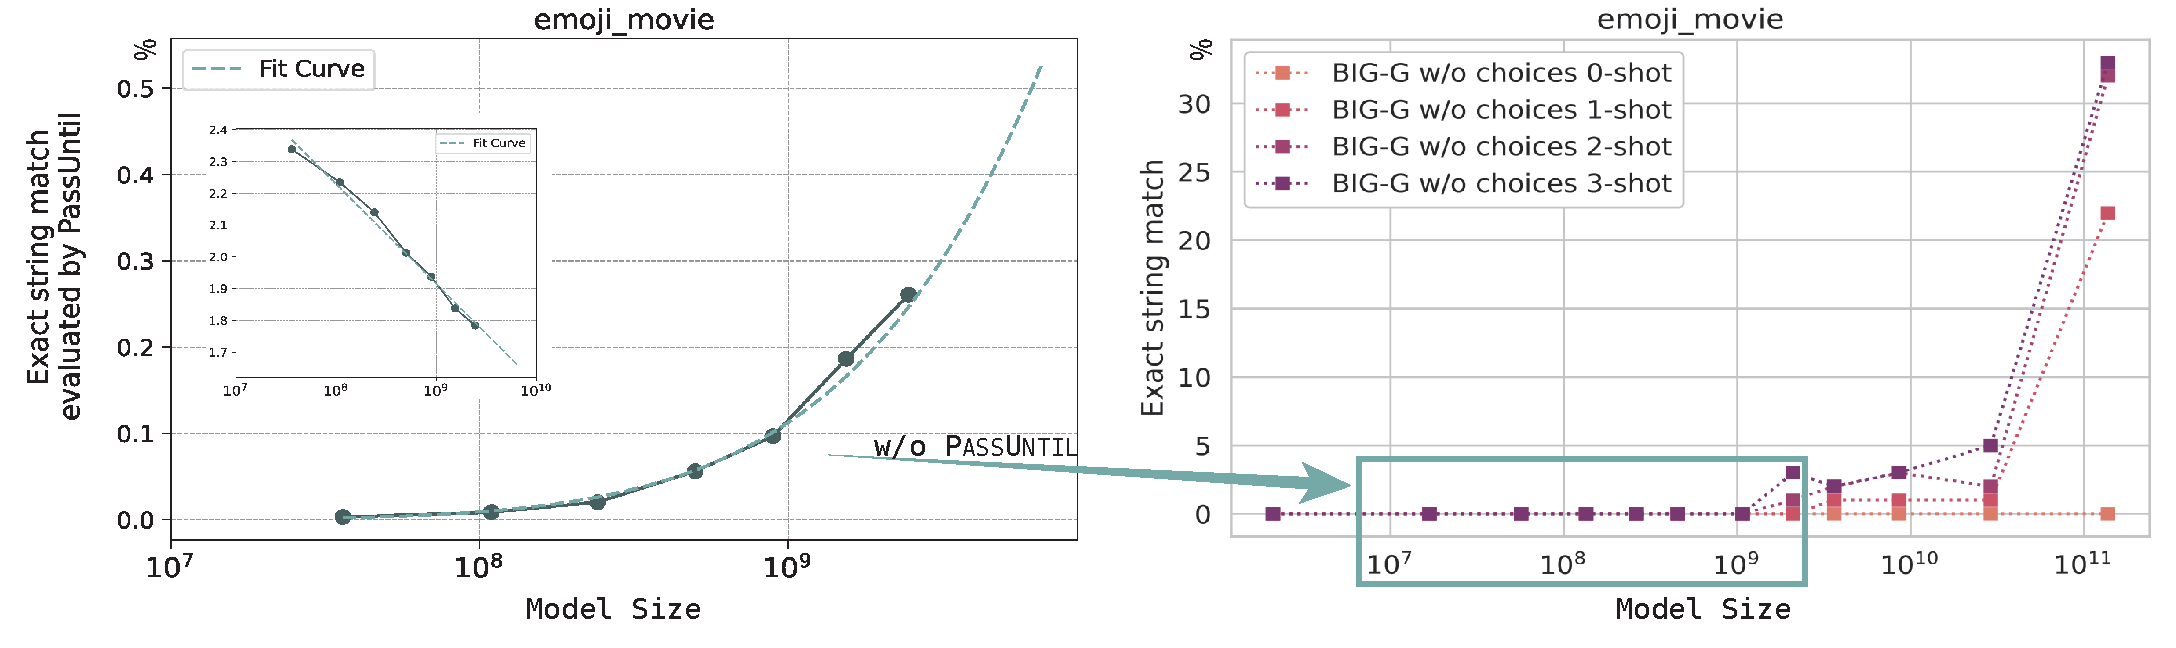
\includegraphics[width=\linewidth]{pufigs/themegraph.pdf}
    \caption{本章节的方法能够辨别出细微的性能提升(左图),而传统方法将其评估为全零(右图)。右图直接采用了 \citet{sorscher2022beyond} 中图9(a) 作为对比。该论文作者用此图来说明任务性能中的 “涌现” 行为。左图中的内嵌图展示了在 $\log(-\log(\cdot))$ 空间中的性能,呈现出很强的线性关系,支持任务扩展定律(公式(\ref{eq:task_scaling_raw}))。}
    \label{fig:themefig}
\end{figure}

将损失扩展定律扩展到任务性能的挑战主要源于扩展过程中任务性能的 “不连续性”。小于一定规模的语言模型表现出微不足道的性能,即在多项选择题中表现为随机猜测或在生成任务中获得零分。然而,当模型规模超过某个阈值时,性能会出现明显的激增,从而带来显著的非平凡性能。这种现象被总结为 “涌现能力” \citep{srivastava2022beyond, wei2022emergent}。这种涌现能力在各种模型系列和任务中都有观察到。似乎模型规模大小 内部发生了质的变化,使得模型开始展现出独特的能力。

虽然这些涌现现象表明大语言模型正在变得更强,但它们使任务性能的预测变得复杂。于是一个关键问题出现了:\textbf{能否从这些明显的不连续性中寻找出任务性能的可预测扩展规律?} 本文假设,从微不足道到卓越性能的这种看似不连续的现象,可能源于有限的评估分辨率。这里的 “分辨率”的意思是:当将评估视为对完成任务真实概率的一种度量时,某种评估策略的分辨率是该评估策略能够检测到的最小概率差异。通过采用更精细的分辨率,有可能揭示任务的扩展定律。 

与本章最相关的工作是 \citet{schaeffer2023emergent},它提出了两种使涌现能力连续化的方法,即 “改变度量” 和通过扩大测试集规模 “提高分辨率”。本文动机与 \citet{schaeffer2023emergent} 的 “改变度量” 方法不同,他们的方法认为采用其他连续度量可能会导致涌现能力消失,而应该使用替代的平滑度量。但是,替代的平滑度量(例如分布距离)的一个局限性在于,它们对评估者直观感知的目标度量(例如完全字符串匹配)提供的洞察力和关联性不足。相比之下,我的方法以一种新颖的方式扩展了 “提高分辨率” 的方法,并且能直接给出对目标度量的估计。

\section{方法设计}
\subsection{增加随机采样数量的先导实验}
\label{sec:pilot}
我通过可视化提高评估分辨率对语言模型的影响来开启探索过程。我选择了四个开源的小模型,并在BigBench任务的两个子集\citep{srivastava2022beyond}:“表情电影”(Emoji Movie)和“日期理解”(Date Understanding)上对它们进行评估。子集详情见\improvement{加上链接}。在解码过程中,我采用束搜索(Beam Search)和随机采样(采样次数分别为1次、100次和10000次)。如果一个测试实例有任何采样答案被评估为正确,那么该实例就被标记为“通过”。图\ref{tab:opensourcemodel_rs}中展示了“通过”的实例数量。

\begin{figure}[htbp]
\centering
    % \begin{tabular}{c|cccc|cccc}
    %     \toprule
    %   \multirow{2}{*}{\textbf{模型}}  & \multicolumn{4}{c|}{\textbf{表情电影}} & \multicolumn{4}{c}{\textbf{日期理解}}\\
    % \cline{2-9}
    %    & \textbf{束搜索} & \textbf{随机采样1次} & \textbf{随机采样100次} & \textbf{随机采样10000次}  & \textbf{束搜索} & \textbf{随机采样1次} & \textbf{随机采样100次} & \textbf{随机采样10000次}  \\
    %     \midrule
    %  Pythia - 410M & 0/41 & 0/41 & 2/41 & 31/41 & 0/50 & 0/50 & 8/50 & 42/50 \\
    %   Pythia - 1.4B & 0/41 & 0/41 & 7/41 & 38/41 & 2/50 & 2/50 & 18/50 & 46/50 \\
    %   OPT - 350M & 0/41 & 0/41 & 4/41 & 33/41 & 1/50 & 0/50 & 4/50 & 37/50 \\
    %   OPT - 1.3B & 0/41 & 0/41 & 12/41 & 39/41 & 1/50 & 1/50 & 12/50 & 46/50 \\
    %    \bottomrule
    % \end{tabular}
    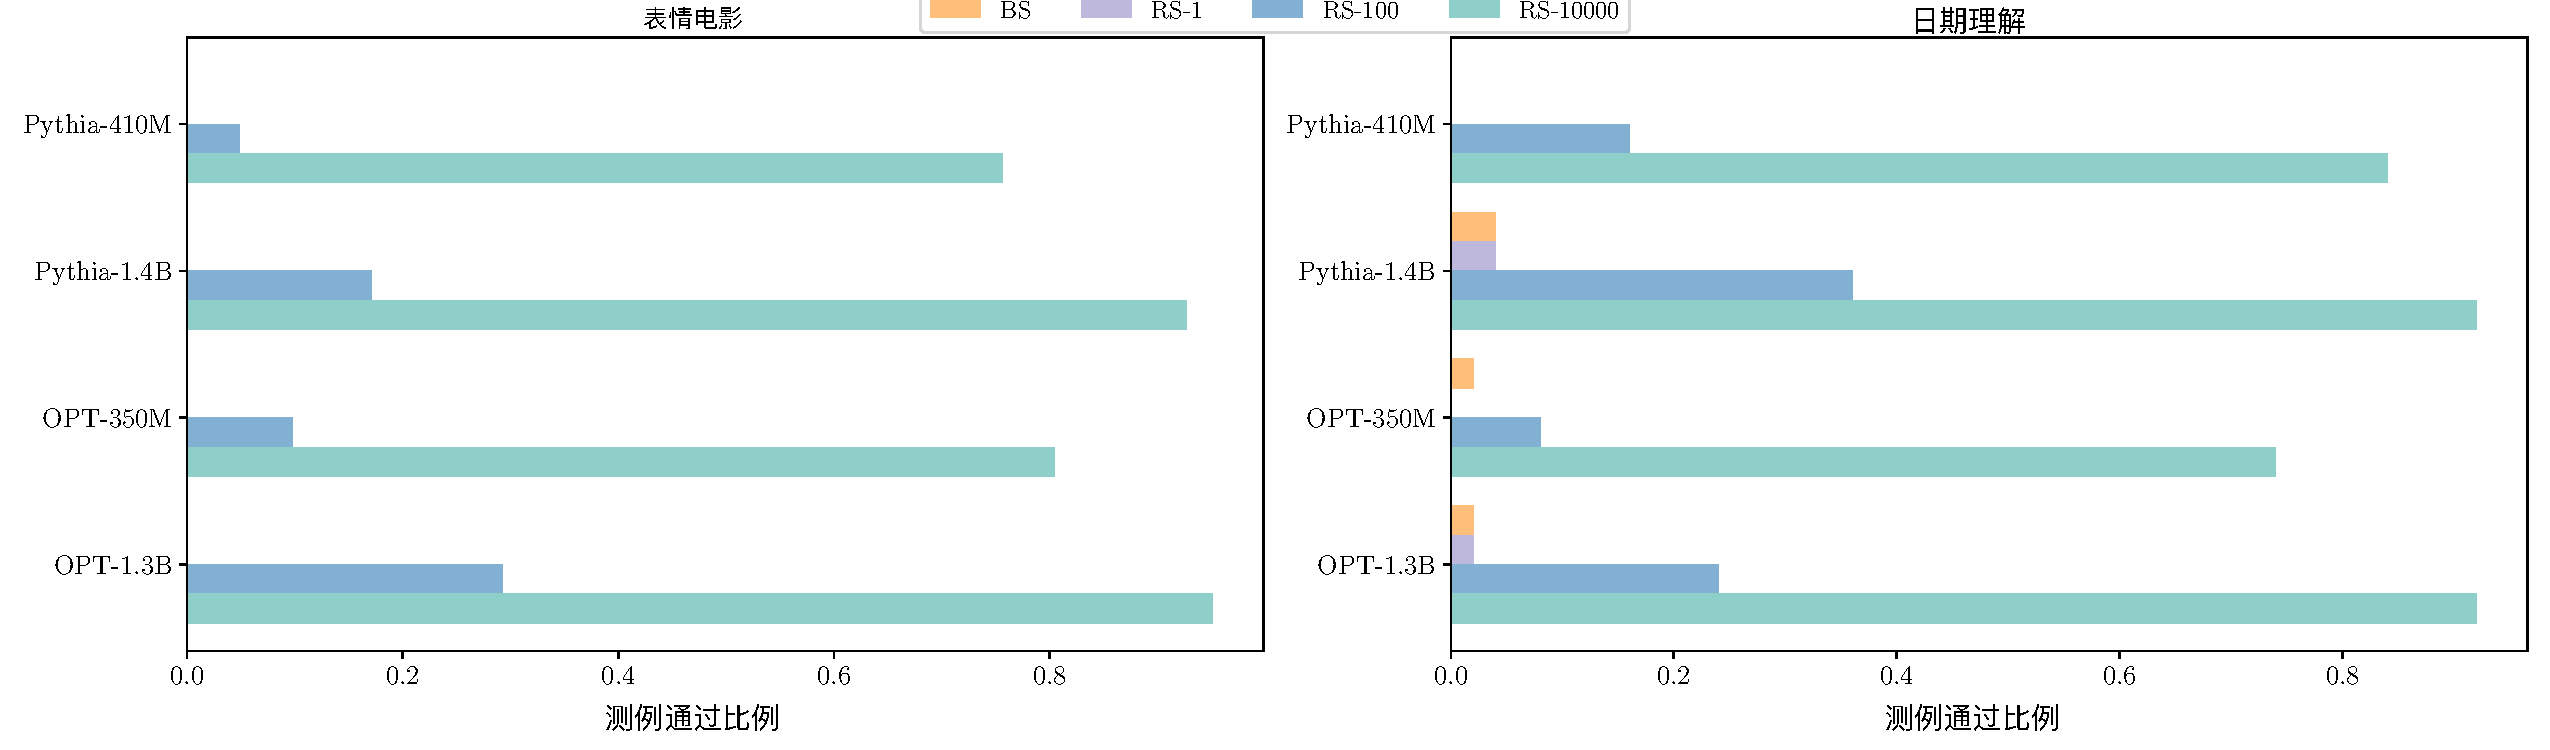
\includegraphics[width=0.98\textwidth]{pufigs/pilot-exp-fig.pdf}
    \caption{BS表示束搜索,RS-$K$表示随机采样$K$次。}
    \label{tab:opensourcemodel_rs}
\end{figure}

可以看到,即使对于这些给小模型带来较大难度的任务,在足够的随机采样次数下,大多数实例都能通过,这将有助于实现细微的任务性能增加。受此观察结果的启发,我提出以提高评估分辨率为核心的评估策略。首先是评估策略“PassUntil”,其次是实例级扩展曲线拟合,此外还有基于损失扩展定律推导出任务扩展定律。 接下来我将具体介绍提高评估分辨率的方法。

\subsection{“PassUntil”实现无限分辨率}
我将任务性能评估视为对模型通过某项任务概率的度量。注意,此处“通过”的定义不一定是要生成和标准答案字符串完全匹配的答案。例如,假设要预测模型在AlpacaEval\citep{alpaca_eval}上的性能,可以将“通过”定义为模型生成的内容优于GPT-4生成的内容。因此,“通过”的定义具有广泛的适用性。给定一个任务实例$s$,假设模型通过它的概率为$P(s)$,现在就是需要估计$\mathbb{E}_s[P(s)]$。随机采样固定次数$K$可以估计$P(s)$。然而,通常很难确定一个在计算上可接受,同时对于$P(s)$较小的困难样本又有足够分辨率的采样次数$K$。我提出“PassUntil”策略,即在生成一个答案后立即进行评估,在采样下一个生成结果之前确定该答案是否通过。持续采样,直到有$r$(一个预先确定的常数)个样本通过评估,并记录采样次数$K$。将$P(s)$的估计值称为“PassUntil”分数$\textsc{PU}$,其定义为:
\begin{equation}
\label{equ:pudef}
    \textsc{PU} = \frac{r}{K}
\end{equation}
从理论上讲,$\textsc{PU}$能够测量极小的成功率。

“PassUntil”具有以下性质。
\begin{theorem}
$\textsc{PU}$是$P(s)$的最大似然估计。
\end{theorem}

\begin{proof}
失败次数$f = K - r$服从成功概率为$P(s)$的负二项分布。而$r/K$是$P(s)$的最大似然估计。
\end{proof}


在实际应用中,考虑到评估效率,我将$r$设置得尽可能小,如$1$。我还将$K$的上限设置为一个较大的数,如$10^5$,以防止在遇到极低的$P(s)$时进行无休止的采样。需要注意的是,许多实例在达到这个上限之前就停止采样了。接下来我将讨论“PassUntil”的必要性和局限性。

\begin{enumerate}
    \item \textbf{必要性}。 一般来说,从理论上根据真实解的词元概率推导出$P(s)$是不可行的。这主要有两个原因:第一,可能存在多个可行解;第二,即使只有一个解,除了最优分词方式外,还有多种解码方式可以解码出该解。例如,在GPT-4的“cl100k-base”词表中,用token序列[4513]、[717,18]和[16,17,18]都可以解码为字符串“123”,这导致标准答案在词元层面并不一定是唯一的,进一步导致通过计算词元概率来得到任意的目标观测指标是不可行的。
    \item \textbf{局限性(1)。} 目前,本文的评估策略设计适用于随机预测的基线能取得0分的得分的目标指标,即$P(s) = 0$的情况。在以多项选择得分作为评估指标的情况下,相对于模型的真实性能,评估结果往往会出现偏高的偏差(例如,对于四个选项的题目,随机猜测的$P(s) = 0.25$)。这种随机噪声可能会掩盖较小模型所取得的改进。对于具有非零随机基线的任务扩展定律的探索仍然是未来研究的课题。
    \item \textbf{局限性(2)。} 由于随机采样在大语言模型中广泛使用,目前本文仅将其视为一种可行的目标解码策略。将束搜索作为目标解码策略及其与随机采样的关系,为未来的探索和研究提供了一个有趣的方向。 
\end{enumerate}


\subsection{任务扩展定律}
接着,我推导出“PassUntil”所遵循的任务扩展定律。假设生成下一个词元的测试损失按照公式(\ref{eq:loss_scaling_law})的扩展定律下降,则“PassUntil” 将可以用如下规律理论推出:
\begin{equation}
\label{eq:task_scaling_raw}
    \textsc{PU} \sim \prod_{i=1}^{|y|} P(y_i|\{x_{1:|x|}, y_{1:i - 1}\}) = \prod_{i=1}^{|y|} \exp(-{c_i}{{N}^{-\alpha_i}} - L_{0i}),
\end{equation}
其中,$x_{1:|x|}$是输入序列,$y_{1:|y|}$是解码出正确答案的最可能序列(假设相较于其他序列,它占主导地位)。
假设给定一个足够强大的大语言模型(LLM),测试样本是可通过的,那么每个词元的不可约损失$L_{0i}$趋近于$0$。并且假设答案中每个词元的测试损失在扩展时以均匀的速度下降(即$\forall i$,$a_i = a$),可以推导出关于任务性能的$\textsc{PU}$的以下函数:
\begin{equation}
\label{eq:exp_scaling}
    \textsc{PU}(c, \alpha; N) \sim \operatorname{exp}(\sum_i -{c_i}{{N}^{-\alpha}} ) = \operatorname{exp}(-{c}{{N}^{-\alpha}})
\end{equation}
其中$c = \sum_i c_i$。值得指出的是,尽管方式不同,但是得到的数学模型与GPT-4技术报告\citep{openai2023gpt4}以及\citet{schaeffer2023emergent}中的公式(4)有共同点。

\subsection{拟合策略}
\textbf{数据集层面的拟合。}在拟合$\textsc{PU}$中的参数$c$、$\alpha$时,数据集层面的拟合是可行的。对于扩展曲线中的第$j$个模型(其参数量大小为$N_j$),首先在测试集上对单个测试样本的$\textsc{PU}$求平均,得到$\operatorname{log}(-\operatorname{log}(\textsc{PU}(N_j)))$,然后对$\operatorname{log}N_j$进行线性回归。

\textbf{实例(instance)层面的拟合。}
\label{sec:instance_level_pass}
本文注意到,测试数据集中不同测试实例(instance,或者称作样本)之间的差异会导致不同的扩展行为。这意味着当测试集内,不同实例的难度不同时,数据集层面的拟合可能不准确。例如,简单问题的$\textsc{PU}$在小模型上就会很快饱和到$1$,而难题仍然表现出微不足道的性能。因此本文进一步提出实例层面的拟合方法:为每个实例拟合一个单独的“PassUntil”分数, 即Instance-level PassUntil($\textsc{IPU}$),并将它们汇总以估计整个数据集的情况。即,假设数据集为$S = \{s\}$, 每个测试实例对应的IPU参数为$c_s, a_s$, 则:
\begin{equation}
    {\textsc{PU}}(\{c_s, a_s\}; N) = \frac{1}{|S|}\sum_s {\operatorname{IPU}}(c_s, a_s; N)
\end{equation}


\section{可预测扩展实验}

在本节中,我将展示所提出的框架在实际实验中的作用。我预训练了两个系列的语言模型,参数规模从3000万(0.03B)到24亿(2.4B)不等。基于系列中其他模型的性能来预测24亿参数模型的性能。

\subsection{实验配置}
\label{sec:train}
\subsubsection{模型配置}
在扩大Transformer模型规模时,需要保持其 “形状” 一致。对于扩展曲线中的第\(i\)个模型,将层数设置为\(4i\),注意力头的数量设置为\(\lfloor \frac{i(8 + i)}{4} \rfloor\),头的维度设置为\(64\)。这使得隐藏状态的维度\(d_m\)为\(d_hn_h\)。我将前馈层的维度设置为\(2.5d_m\)。具体数值列于表\ref{tab:pu_model_configs}中的模型配置里。该架构与LLaMA类似\citep{touvron2023llama}。一些细微差异包括:我在输入和输出嵌入之间使用共享嵌入,并且使用门控高斯误差线性单元(gated-GeLU)\citep{hendrycks2016gaussian} 替代门控SiLU\citep{DBLP:journals/corr/abs-2002-05202}。

\begin{table}[htbp]
    \centering
    \caption{扩展曲线中各模型的模型配置和训练配置。N(十亿)表示模型的非嵌入参数数量,单位为十亿。BS(百万)表示用于训练模型的每个批次中的令牌数(即批量大小),单位为百万。TS表示训练步数。令牌数(十亿)指用于训练模型的令牌总数。}
\scalebox{0.9}{
    \begin{tabular}{c|cccccccccc}
    \toprule
        名称 & i & N(十亿)& $d_m$ & $d_{ff}$ & $d_h$ & $n_h$ & $L$ & BS(百万) & TS & 词元数(十亿)\\
    \midrule
  $\backslash$ & i & $\backslash$ & $d_hn_h$ & $2.5d_{m}$ & 64 & $\lfloor \frac{i(8 + i)}{4} \rfloor$ & $\lfloor4i\rfloor$ & $\backslash$ & $\backslash$ & $\backslash$\\
           0.03B & 3 &  0.036 & 512 & 1280 & 64 & 8 & 12 & 0.33 & 2196 & 0.72\\
          0.1B & 4 & 0.109 & 768 & 1920 & 64 & 12 & 16  & 0.88 & 2464 & 2.18\\
         0.2B & 5 & 0.241 & 1024 & 2560 & 64 & 16 & 20  & 1.57 & 3064 & 4.82\\
        0.5B & 6 & 0.499 & 1344 & 3360 & 64 & 21 & 24 & 2.10 & 4758 & 9.99\\
        0.9B & 7 & 0.892 & 1664 & 4160 & 64 & 26 & 28  & 2.95 & 6049 & 17.9  \\
        1.5B & 8 & 1.542 & 2048 & 5120 & 64 & 32 & 32 & 4.26 & 7230 & 30.8\\
       2.4B & 9 & 2.45 & 2432 & 6080 & 64 & 38 & 36 & 5.51 & 8900 & 49.0\\
    \bottomrule
    \end{tabular}
}
    \label{tab:pu_model_configs}
\end{table}



\subsubsection{预训练语料库}
对于系列一,我在单目标任务(即代码生成任务)上进行评测, 因此使用单源预训练预料——StarCoder数据集\citep{li2023starcoder}——作为预训练数据。对于系列二,我在多目标任务上进行评测,使用StarCoder和Pile数据集\citep{gao2020pile}的混合数据。利用最优计算大语言模型的方法\citep{hoffmann2022training},我将每个模型规模的最大预训练词元数设置为\(20N\),其中\(N\)是模型的非嵌入参数数量。表\ref{tab:series1_data_mixture}和表\ref{tab:series2_data_mixture}分别展示了系列1和系列2大语言模型的具体数据混合比例。


\begin{table}
        \centering
        \caption{系列一模型的预训练语料。}
        \begin{tabular}{c|c}
        \toprule
           语料库   &  词元占比 \\
        \midrule
        StarCoder\_Python &  0.3\\
        StarCoder\_Others &  0.7\\
    \bottomrule
        \end{tabular}
        \label{tab:series1_data_mixture}
    \centering
\end{table}

\begin{table}
    \centering
    \caption{系列二模型的预训练语料}
    \begin{tabular}{c|c}
    \toprule
       语料库   &  词元占比 \\
    \midrule
    StarCoder\_Python &  0.15\\
    StarCoder\_Others &  0.12\\
    Stack\_Overflow & 0.03 \\
    Arxiv & 0.05 \\
    Pile & 0.65 \\
\bottomrule
    \end{tabular}
    \label{tab:series2_data_mixture}
\end{table}


\subsubsection{超参数设置}
\label{app:hyperparameters}
\textbf{学习率}:采用余弦退火学习率调度器,与之前的研究\citep{touvron2023llama, touvron2023llama2, hoffmann2022training}类似。在不同的模型规模下,最大学习率始终固定为\(0.01\),在此学习率下没有出现明显的损失爆炸情况。这种稳定性可能归因于前面几章提到的归一化策略\citep{yang2022tensor}以及跨规模增加的批量大小。如前文所述,与\citet{hoffmann2022training}的研究结果一致,我研究得到对于训练大语言模型直至特定的结束步数,余弦退火学习率调度器的最优循环长度应等于结束步数。偏离此最优循环长度,无论是变长还是变短,都会导致性能次优。

\textbf{批量大小}:为了估计模型预训练所需的最优批量大小,我按照\citet{kaplan2020scaling}的方法重复实验,以确定模型的最优批量大小,并在最优批量大小的基础上对实际批量大小进行微调,以最大化GPU利用率。批量大小和训练步数的值列于表\ref{tab:pu_model_configs}中。 

\subsubsection{测试集配置}
\label{app:testset}
在本小节中,我介绍实验中的测试集和评估细节。
\paragraph{HumanEval}
\label{app:humaneval}
OpenAI发布的HumanEval\citep{chen2021evaluating}数据集包含164个编程问题。每个问题由一个函数签名、一个文档字符串、一个函数体和多个单元测试组成。我对该数据集采用零样本方法进行评估。只有当大语言模型生成的代码成功通过所有单元测试时,才认为代码完成通过。在我的评估中,将“PassUntil”中的采样次数上限设置为\(10^4\)。

\paragraph{表情电影(Emoji Movie)}
\label{app:emoji_movies}
“表情电影”是评测集合BigBench\citep{srivastava2022beyond}中的一个子任务,要求大语言模型根据用表情符号描述的情节识别知名电影。评估方法结合了思维链(Chain-of-Thought,CoT)和四样本上下文学习。我从原始的50个实例中选择41个测试实例(剔除了9个干扰实例,详见章节\ref{app:removing_distracting})构成测试集,并任意指定4个实例作为少样本上下文。使用GPT-4为这些上下文样本的产生思维链,并期望模型能读取这四个上下文样本的思维链示例,对测试样本生成一段思考过程,然后给出答案。评估方法采用提取字符串匹配,即模型的输出包含目标电影名称。我将采样次数上限设置为\(10^5\)。 

\paragraph{日期理解}
\label{app:dateunderstanding}
“日期理解” 也是评测集合BigBench\citep{srivastava2022beyond}的一个子集,旨在通过提出与日期推理相关的问题,评估大语言模型理解日期的能力。
对于此任务的评估,我同样采用四样本上下文学习。从原始的50个实例中随机抽取47个实例组成测试集(剔除了3个干扰实例,详见章节\ref{app:removing_distracting})。从剩余数据集中随机抽取4个实例作为上下文示例。同样使用提取字符串匹配的方式来衡量大语言模型的输出,并将采样次数上限设置为\(10^5\)。

\paragraph{非自然上下文学习任务}
\label{app:unantural_in_context_learning}
非自然上下文学习任务是BigBench\citep{srivastava2022beyond}中一系列独特的子任务。这些子任务旨在评估模型在上下文序列被有意改变为可能超出训练数据分布的情况下进行上下文学习的能力,这要求模型关注非传统的上下文模式。表\ref{tab:unnaturalincontextexample}列举了这些子任务的一些实例。
对于每个任务,采用4样本上下文学习配置,从数据集中随机抽取20个实例组成测试集。从剩余数据集中随机选择4个实例作为上下文。我使用提取字符串匹配的方式来衡量大语言模型的输出,并将采样次数上限设置为\(10^5\)。

\begin{table}[!htbp]
    \centering
    \label{tab:unnaturalicl}
    \caption{非自然上下文学习任务中的示例任务}
    \begin{tabular}{p{4cm}l}
        \toprule
        \textbf{任务名称}  & \textbf{示例} \\
        \midrule
        日期  & 输入: 2015-10-22\ 目标: \textit{!10!22!2015!}\\
        非自然格式日期  & 输入:!08!24!1984!\ 目标: \textit{1984-08- 24}\\
        非自然内容日期  & 输入: 96980-49665-10674\ 目标: \textit{!49665!10674!96980!}\\
        非自然格式与内容日期  & 输入:!49665!10674!96980!\ 目标: \textit{96980-49665-10674}\\
        原样输出  & 输入: a, b, c, d, e\ 目标: \textit{a, b, c, d, e} \\
        反转自然内容  & 输入: t, u, o, b, a\ 目标: \textit{a, b, o, u, t} \\
        反转成自然内容  & 输入: r, o, o, m, s\ 目标: \textit{s, m, o, o, r}  \\
        两位数运算  & 输入: 10 - 10 =\ 目标: \textit{20}\\
        \bottomrule
    \end{tabular}
    \label{tab:unnaturalincontextexample}
\end{table}



\subsection{损失扩展定律验证}
图\ref{fig:loss_scaling}展示了各模型的训练损失曲线。显然,最终训练损失按照扩展定律下降。这些通过实证观察得到的损失扩展定律,为后续对任务性能的近似分析奠定了基础。需要注意的是,尽管15亿和24亿参数的模型出现了损失尖峰,但最终仍收敛到扩展定律,这体现了该经验定律的稳健性。


\begin{figure}[!htbp]
        \centering
        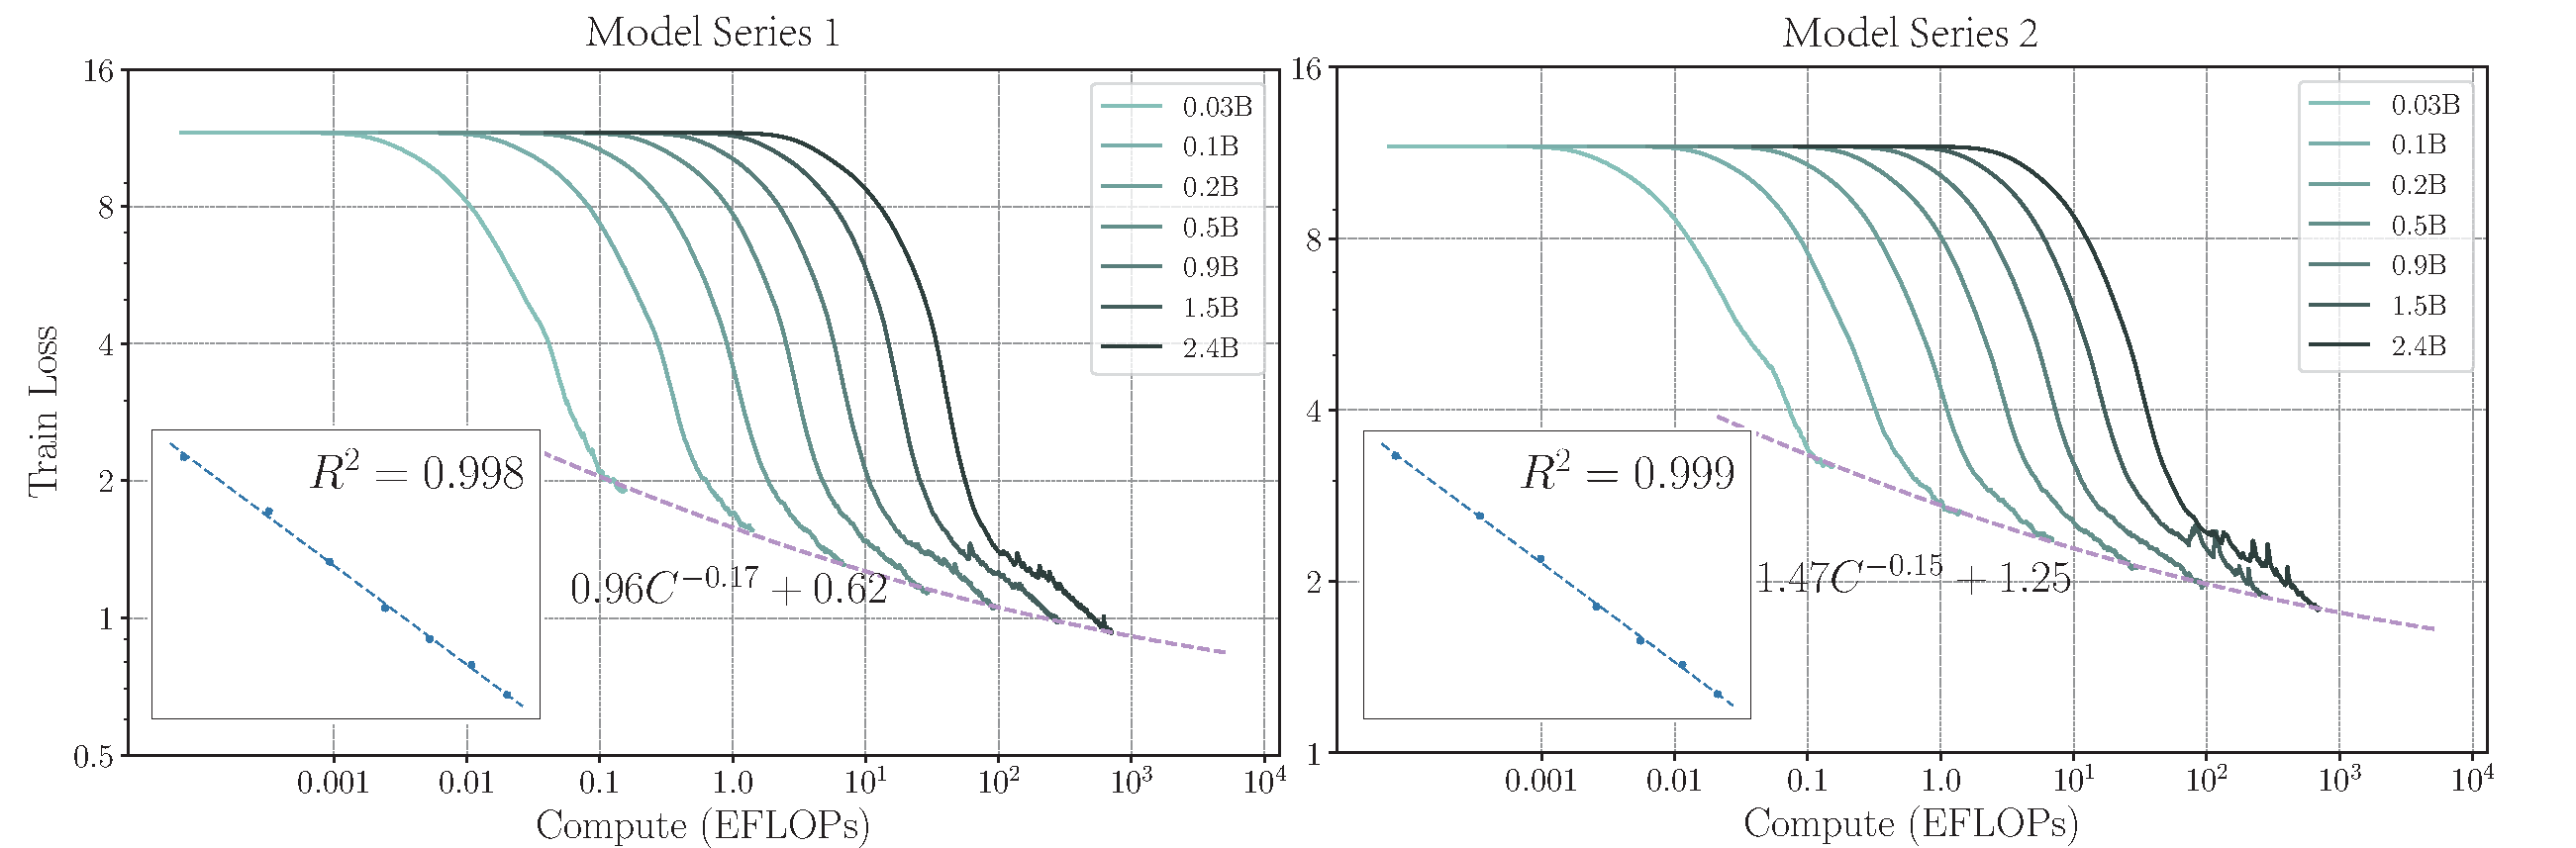
\includegraphics[width=0.85\linewidth]{pufigs/train_loss_2series.pdf}
        \label{fig:train_loss_2series}
\caption{在不同数据混合上训练的两个系列模型的训练损失。内插图展示了相对于模型规模的最终步骤可约损失,以对数尺度表示。 }
    \label{fig:loss_scaling}
\end{figure}



\subsection{去除干扰因素}
\label{app:removing_distracting}
我注意到,在测量模型规模扩展过程中的微小性能提升时,去除干扰因素至关重要。干扰因素指的是某个测试实例在所需能力或评估偏差方面与其他测试实例存在显著差异。请注意,我基于对测试实例的观察来选择干扰因素,这在预测24亿参数模型时不会导致信息泄露。

举例说明如下:对于“表情电影”任务,由于采用提取字符串匹配的评分方式,即模型答案是否正确取决于其输出中是否包含电影名称,而部分电影名称是常用词,这使得即使是规模较小的模型也能根据评估标准“猜出”正确答案。我找出了电影名字是常见单词或词组的实例,如图\ref{fig:emoji_common_words}所示,不同规模模型在这些实例上的通过率没有显著关联。换句话说,扩展定律对这些问题的模型性能影响不大。因此,将此类干扰因素排除在外就变得至关重要。我剔除了流行工具包NLTK识别出的常用词形式的电影名称\footnote{\url{https://www.nltk.org/}}。

对于“日期理解”任务,我省略了表\ref{tab:du_distracting}中所示的以下实例。这些实例仅要求模型从上下文中提取答案,而不要求对日期进行推理。这是和本文关心的目标能力是两种不同的能力,如果混杂在一起评测只会导致混乱的结论。

在GPT-4报告\citep{openai2023gpt4}中,他们将HumanEval数据集按不同难度分成单独的区间,并对每个区间进行扩展预测,从而消除了简单示例对困难示例的干扰。

\begin{table}[!htbp]
\centering
\caption{“日期理解”任务中的干扰实例。}
\scalebox{0.9}{
    \begin{tabular}{p{13cm}}
        \toprule
      \textbf{示例} \\
        \midrule
         今天的会议重新安排到明天上午11点,1924年10月16日。明天的日期(格式为MM/DD/YYYY)是什么? \\
         \hline
         昨天是1929年12月31日。今天不可能是1929年12月32日,因为12月只有31天。昨天的日期(格式为MM/DD/YYYY)是什么? \\
        \hline
        今天是9月7日。简正在观看2003年的美国国家橄榄球联盟(NFL)比赛。今天的日期(格式为MM/DD/YYYY)是什么? \\ 
    \bottomrule
    \end{tabular}
}
    % \label{tab:unnaturalicl}
    \label{tab:du_distracting}
\end{table}

\begin{figure}[h]
    \centering
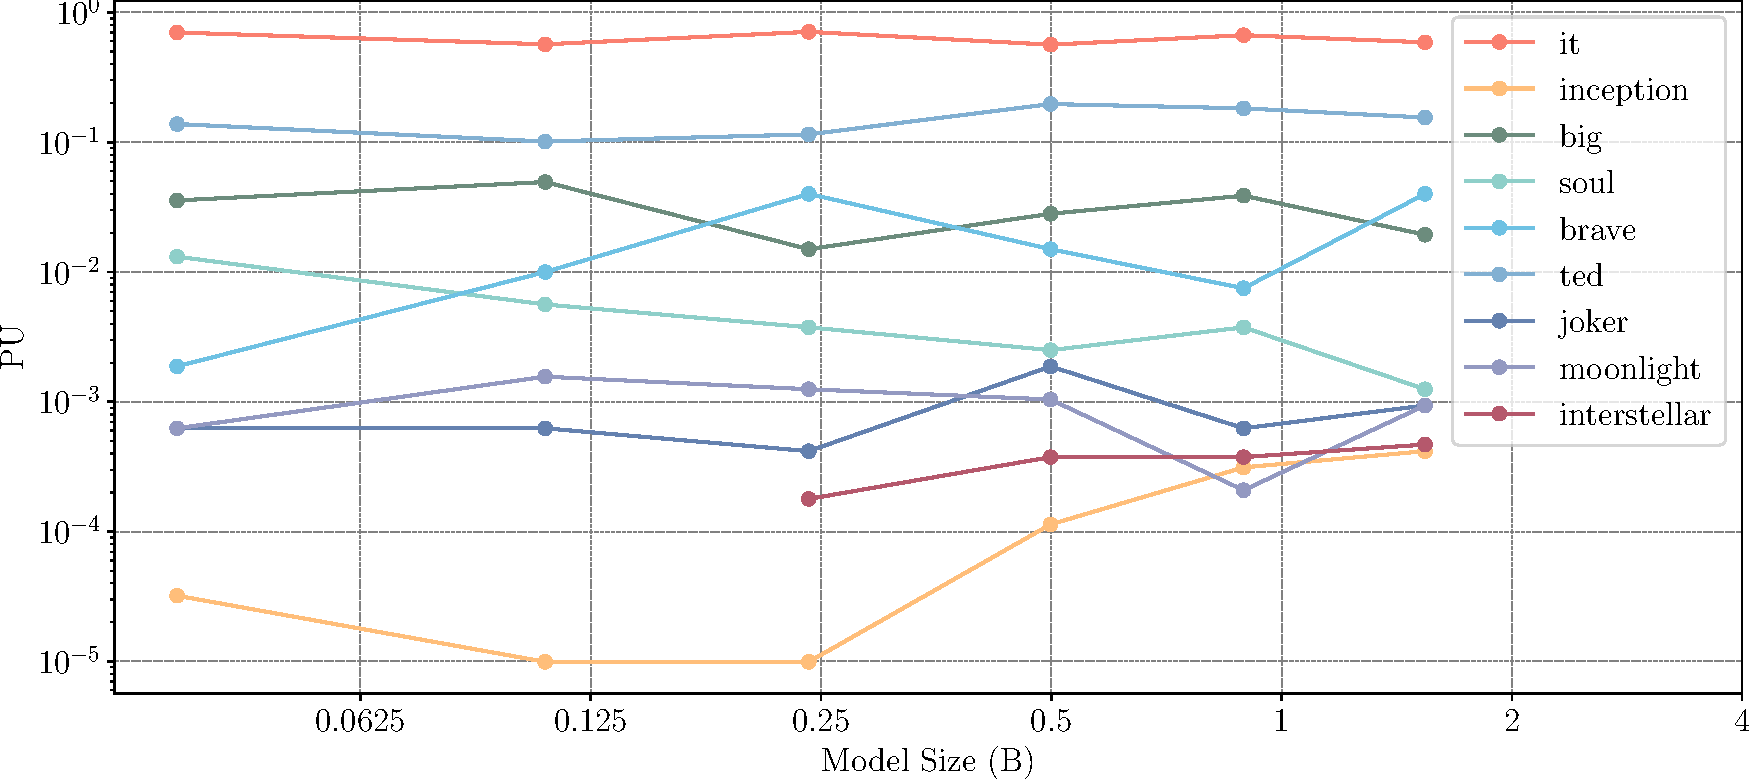
\includegraphics[width=0.85\linewidth]{pufigs/emoji_removing_distracting.pdf}
\caption{在这些实例上,大模型和小模型的 \textsc{PU} 相似(主要是因为从词汇空间中随机采样),这在实验中造成了干扰。}
    \label{fig:emoji_common_words}
\end{figure}



\subsection{数据集层面的拟合}
我选择了HumanEval\citep{chen2021evaluating}、“表情电影”(Emoji Movie)以及“日期理解”(Date Understanding)\citep{srivastava2022beyond}作为评估任务。
需注意,“表情电影” 通常被视为 “涌现能力” 的代表\citep{srivastava2022beyond}(见图\ref{fig:themefig}中的右图)。


\begin{figure}[!htbp]
        \centering
        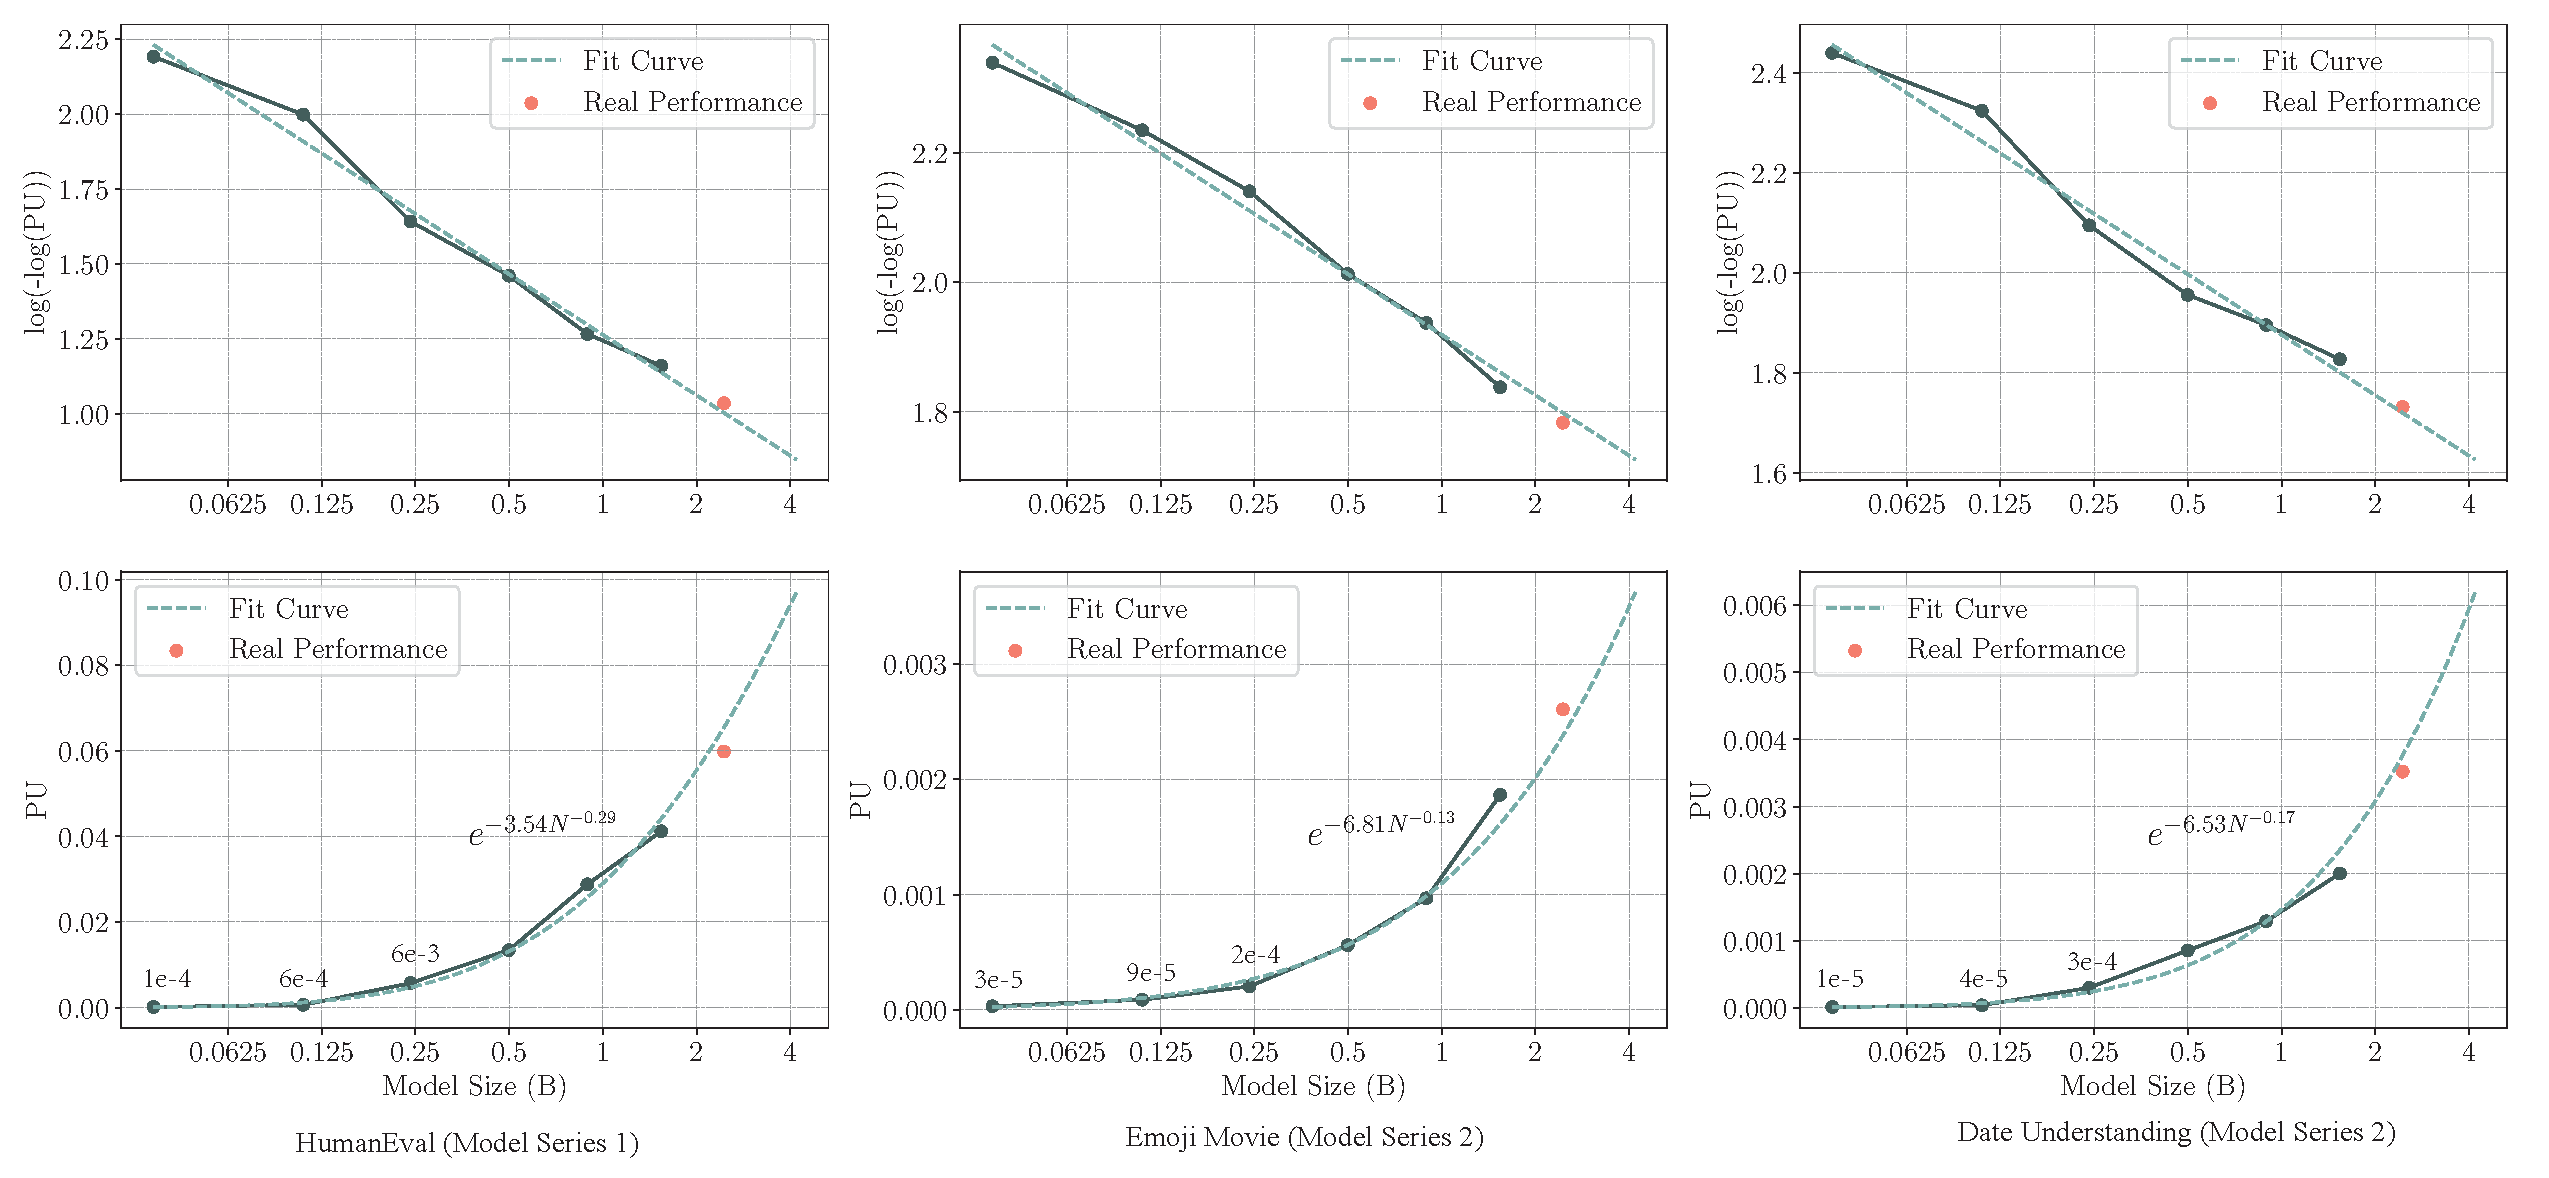
\includegraphics[width=\linewidth]{pufigs/dataset_level_prediction_du.pdf}
        \caption{任务性能随模型规模可预测地扩展。{\color[rgb]{0.85,0.25,0.25}红色}点表示24亿参数模型的实际性能,其与从3000万到15亿参数模型拟合出的任务扩展定律接近。}
    \label{fig:dpu}
\end{figure}

可以观察到,这三个任务在 $\log(-\log(\textsc{PU}))$ 与 $\log(N)$ 之间均呈现出很强的线性关系,从而验证了公式(\ref{eq:task_scaling_raw})所给出的任务扩展定律的有效性。扩展定律函数的估计是利用参数规模从3000万到15亿的模型进行的,利用这些模型对24亿参数模型性能的预测,虽有偏差但在可接受范围内。




\subsection{实例级拟合}

表\ref{tab:easyhardinstances} 展示了HumanEval中一个简单实例和一个具有挑战性实例的“PassUntil”情况。可以观察到,随着模型规模增大,较简单的实例(索引24)呈现出更高的“PU”。然而,更具挑战性的实例(索引20)性能仍然不佳,这表明它们各自的缩放曲线可能存在差异。盲目地对实例的性能进行平均,会使困难实例相对于简单实例的性能提升被掩盖,导致在模型在简单实例上达到饱和后,预测结果不准确。

\begin{table}[h]
    \centering
    \caption{在HumanEval中,简单实例(索引24)相比困难实例(索引20)具有高得多的 $\textsc{PU}$。}
    \begin{tabular}{c|cccccc}
    \toprule
        \multirow{2}{*}{\textbf{实例索引}}  & \multicolumn{6}{c}{\textsc{PassUntil}}   \\
        \cline{2 - 7}
        & \textbf{0.03B} & \textbf{0.1B} & \textbf{0.2B} & \textbf{0.5B} & \textbf{0.9B} & \textbf{1.5B} \\
        \midrule
        20 & 0 & 0 & 0 & 0.000625 & 0.001875 & 0.008125 \\
        % \hline
        24 & 0.00375 & 0.05125 & 0.350625 & 0.3625 & 0.568125 & 0.796875 \\
         \bottomrule
    \end{tabular}
    \label{tab:easyhardinstances}
\end{table}

因此,根据 \ref{sec:instance_level_pass},我考虑了测试样本之间的差异以改进估计。图 \ref{fig:idp_with_modelsize_part1} 中绘制了实例级“PassUntil”的扩展情况。
拟合曲线表明,不同实例的性能不仅起始点不同,而且扩展速度也各异。
尽管如此,它们各自都能通过任务扩展定律进行拟合。部分实例偏离了扩展定律,这有待未来进一步研究。 


\begin{figure}[htbp]
    \centering
    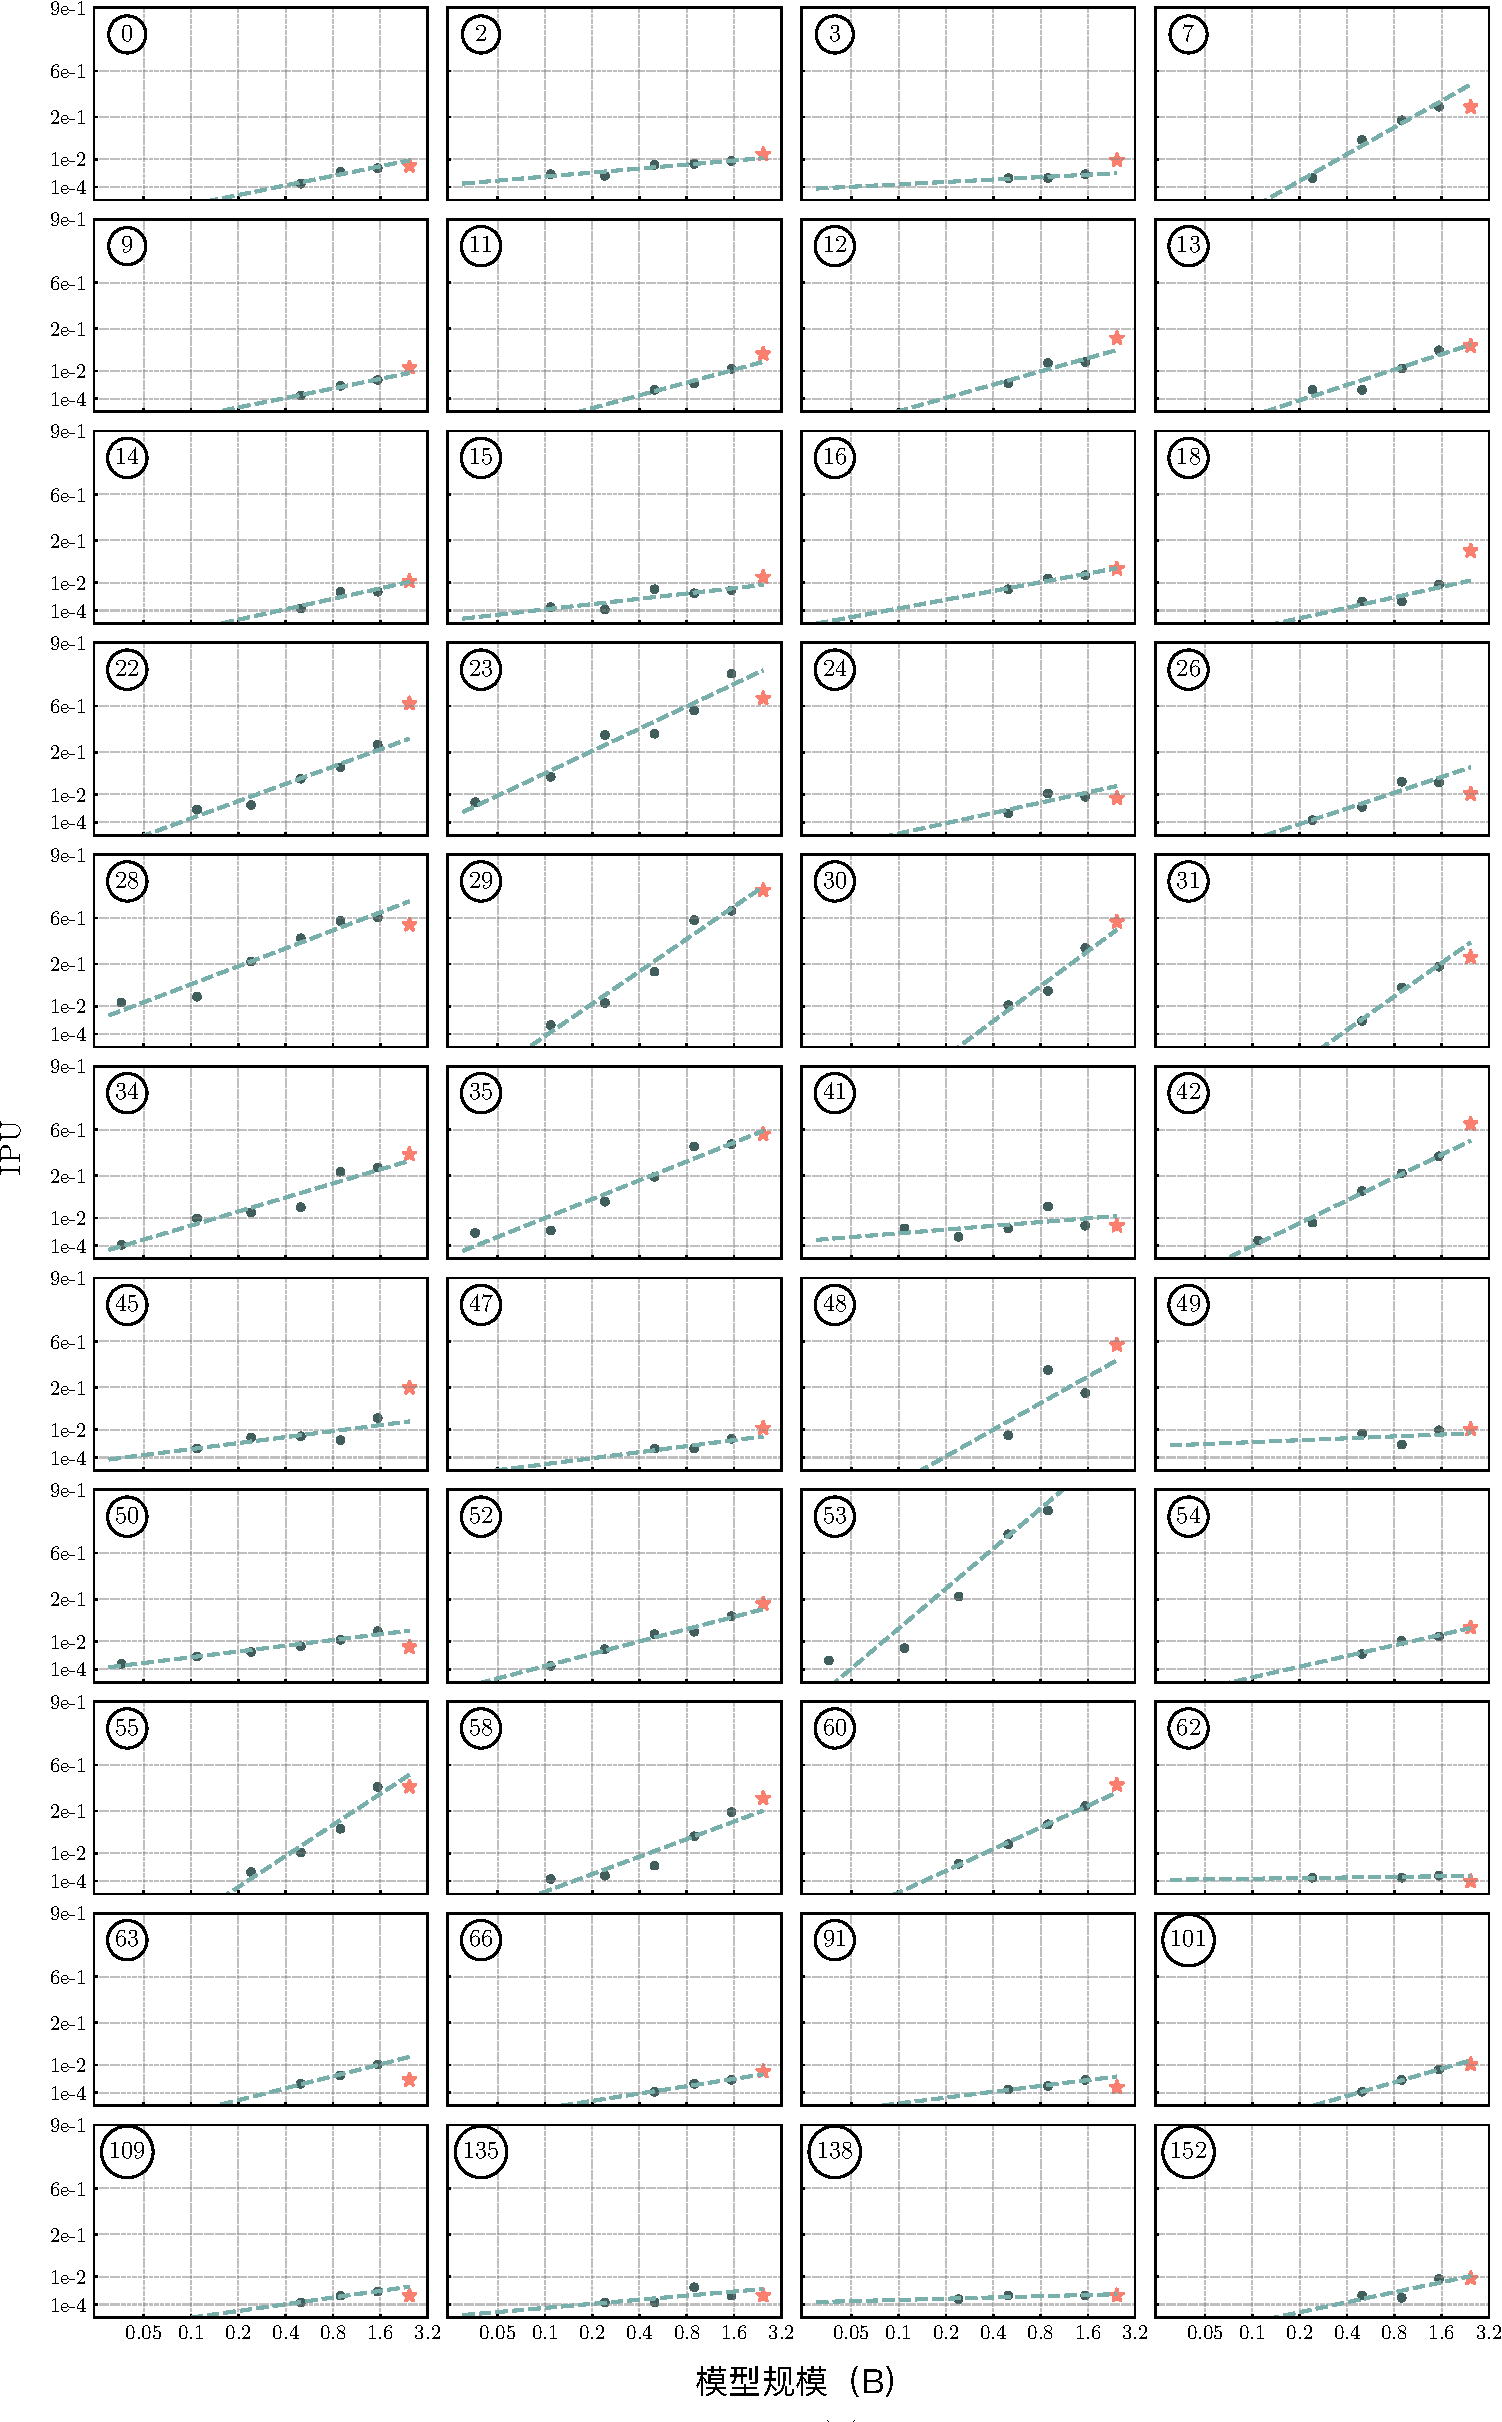
\includegraphics[width=0.85\textwidth]{pufigs/individual_passrate_vs_modelsize_part_main.pdf}
    \label{fig:idp_with_modelsize_part1}
    \caption{实例级扩展定律拟合结果:展示了系列1模型在Humaneval任务上更多单个“PassUntil”扩展曲线的实例。每个子图左上角的标签表示测试集中样本的索引。}
\end{figure}

\begin{figure}[!htbp]
    \centering
    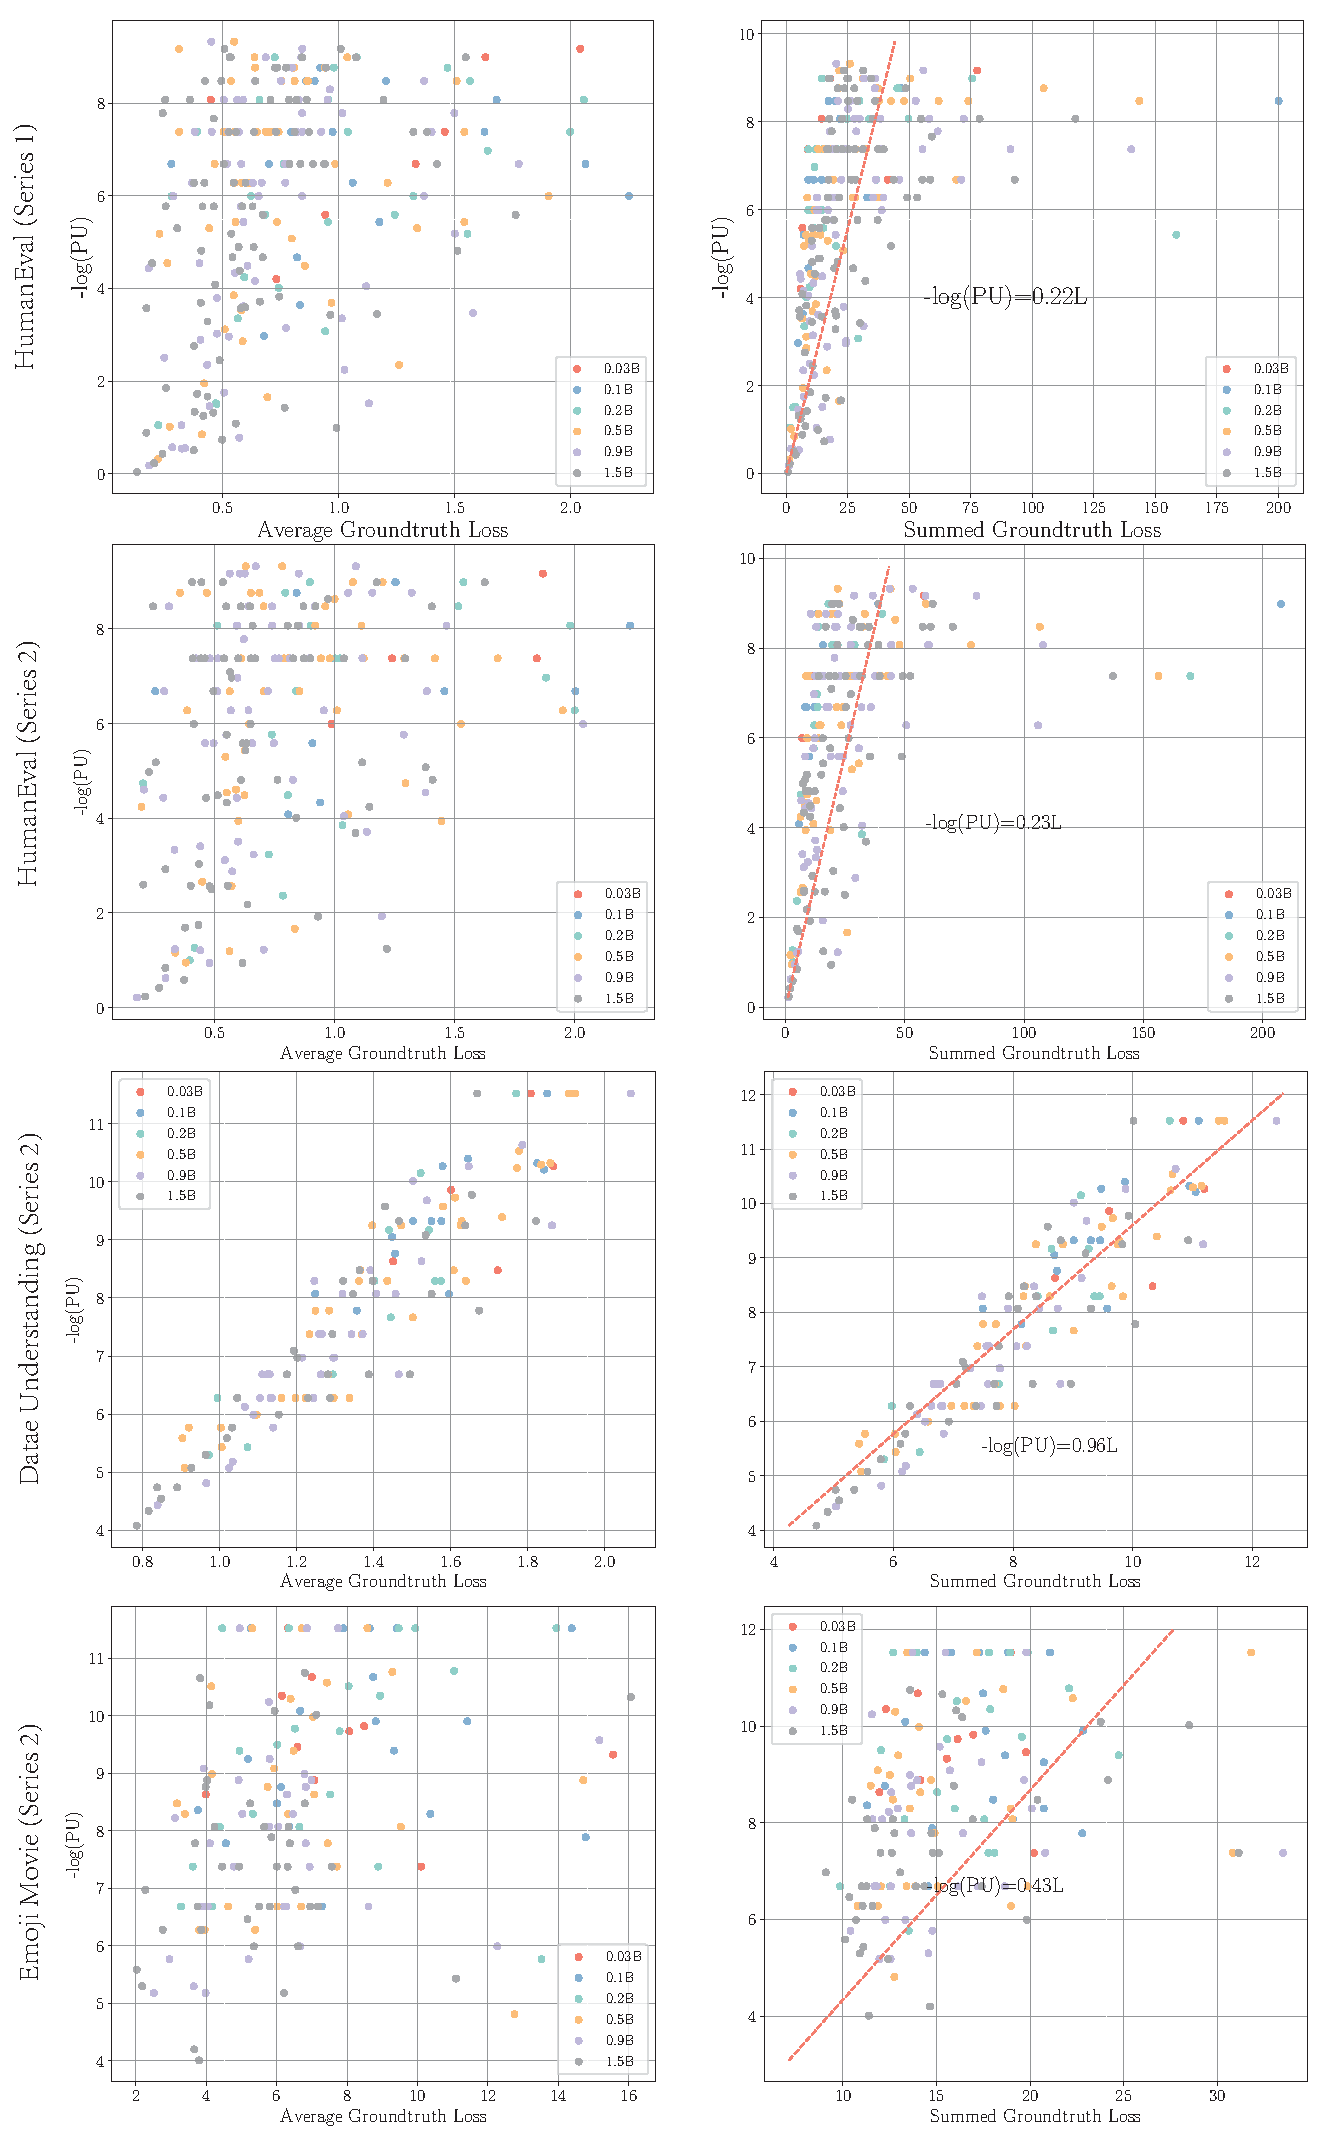
\includegraphics[width=0.8\linewidth]{pufigs/Loss_vs_passuntil.pdf}
    \caption{关于测试损失与“PassUntil”之间关系图。}
\label{fig:loss_vs_passuntil}
\end{figure}

\subsection{从测试损失估计 “PassUntil”}

在实例层面进行估计时,对于难以拟合的实例(即缺乏足够的非零 “PassUntil”值)会面临挑战。随着模型规模的增加,这些样本也可能对 \textsc{PU} 有贡献。因此,本文建议利用真实答案的测试损失来辅助对这类实例的预测。我利用既具有测试损失又有非零 \textsc{PU} 的 “简单” 实例来估计测试损失与 \textsc{PU} 之间的关系(图 \ref{fig:loss_vs_passuntil})。然后,我基于参数规模从3000万到15亿的模型来预测24亿参数模型上每个实例的测试损失。最后,根据上述关系将预测的测试损失转换为预测的 \textsc{PU}。
如图\ref{fig:loss_vs_passuntil}所示,我提出利用真实答案的测试损失来辅助对“困难样本”的预测。对于系列一模型和HumanEval任务,发现其线性关系为\(\textsc{PU} \sim 0.22L\)。对于系列2模型和HumanEval任务,发现线性关系为\(\textsc{PU} \sim 0.23L\)。对于系列2模型和“日期理解”任务,发现线性关系为\(\textsc{PU} \sim 0.96L\)。而对于系列2模型和“表情电影”任务,发现线性关系为\(\textsc{PU} \sim 0.43L\)。 


\begin{table}[!htbp]
    \centering
    \caption{本文任务性能可预测框架的效果:预测值与模型实际性能的预测对比。任务名称后的数字表示评估中使用的模型系列。}
    \scalebox{0.86}{
        \begin{tabular}{lcccc}
            \toprule
            \textbf{方法}  & {\textbf{HumanEval (1)}} & {\textbf{HumanEval (2)}} & {\textbf{Date Understanding (2)}} & {\textbf{Emoji Movie (2)}} \\
            \midrule
            真实值 & 0.05990 & 0.04279 & 0.00346 & 0.002608 \\
            \hline
            数据集层面的拟合 & 0.06550 & 0.05191 & 0.00377 & \textbf{0.002381}\\
            实例层面的拟合 & \textbf{0.05987} & \textbf{0.04402} &\textbf{ 0.00352} & 0.003112\\
            \bottomrule
        \end{tabular}
    }
    \label{tab:final_fit_result}
\end{table}



表\ref{tab:final_fit_result} 中给出了24亿参数模型的最终预测结果,并在图 \ref{fig:final_curve_humaneval_series1} 中绘制预测的 \textsc{PU} 曲线。可以看到,预测结果是准确的,在系列1的HumanEval任务上仅存在0.05\% 的差异,在系列2的 “日期理解” 任务上存在1.7\% 的差异。 


上面使用基于真实标签的损失来辅助“PassUntil”,这可能会引发一种误解:为什么不直接用损失来预测性能呢?下面我详细说明。
\begin{enumerate}
    \item {需要明确区分“损失无法预测任务性能”与“损失有助于预测任务性能”这两种说法。前者指的是在没有其他衡量指标的情况下,仅靠损失不足以用来估计任务性能;而后者表明损失是提高预测准确性的有用因素之一。在本章节中,对这两种说法都进行了明确验证。若不使用“PassUntil”方法,仅从损失值无法推断实际性能(准确率)。例如,损失为1.0并不直接意味着某项任务的准确率为0.2。实际性能必须通过实证测量得到。此外,如图\ref{fig:loss_vs_passuntil}所示,单个样本的损失与“PassUntil”结果并非一一对应,与离散的准确率更是如此。}
    \item {然而,损失确实能提供有用信息。一旦在大量样本集中测量“PassUntil”,就可以建立损失与“PassUntil”之间的统计关系(仅依靠损失数据则无法做到)。这种关系能够提高预测准确性。}
    \item {将损失纳入以改进预测是出于实际考虑,比如计算资源有限,而非必要之举。图\ref{fig:dpu}表明,即使没有损失数据,也能准确预测任务性能。设想一下,如果能够以足够的分辨率测量每个样本,确保每个样本至少通过一次,在这种情况下,损失数据就并非必需。}
\end{enumerate}


\begin{figure}[!htbp]
    \centering
    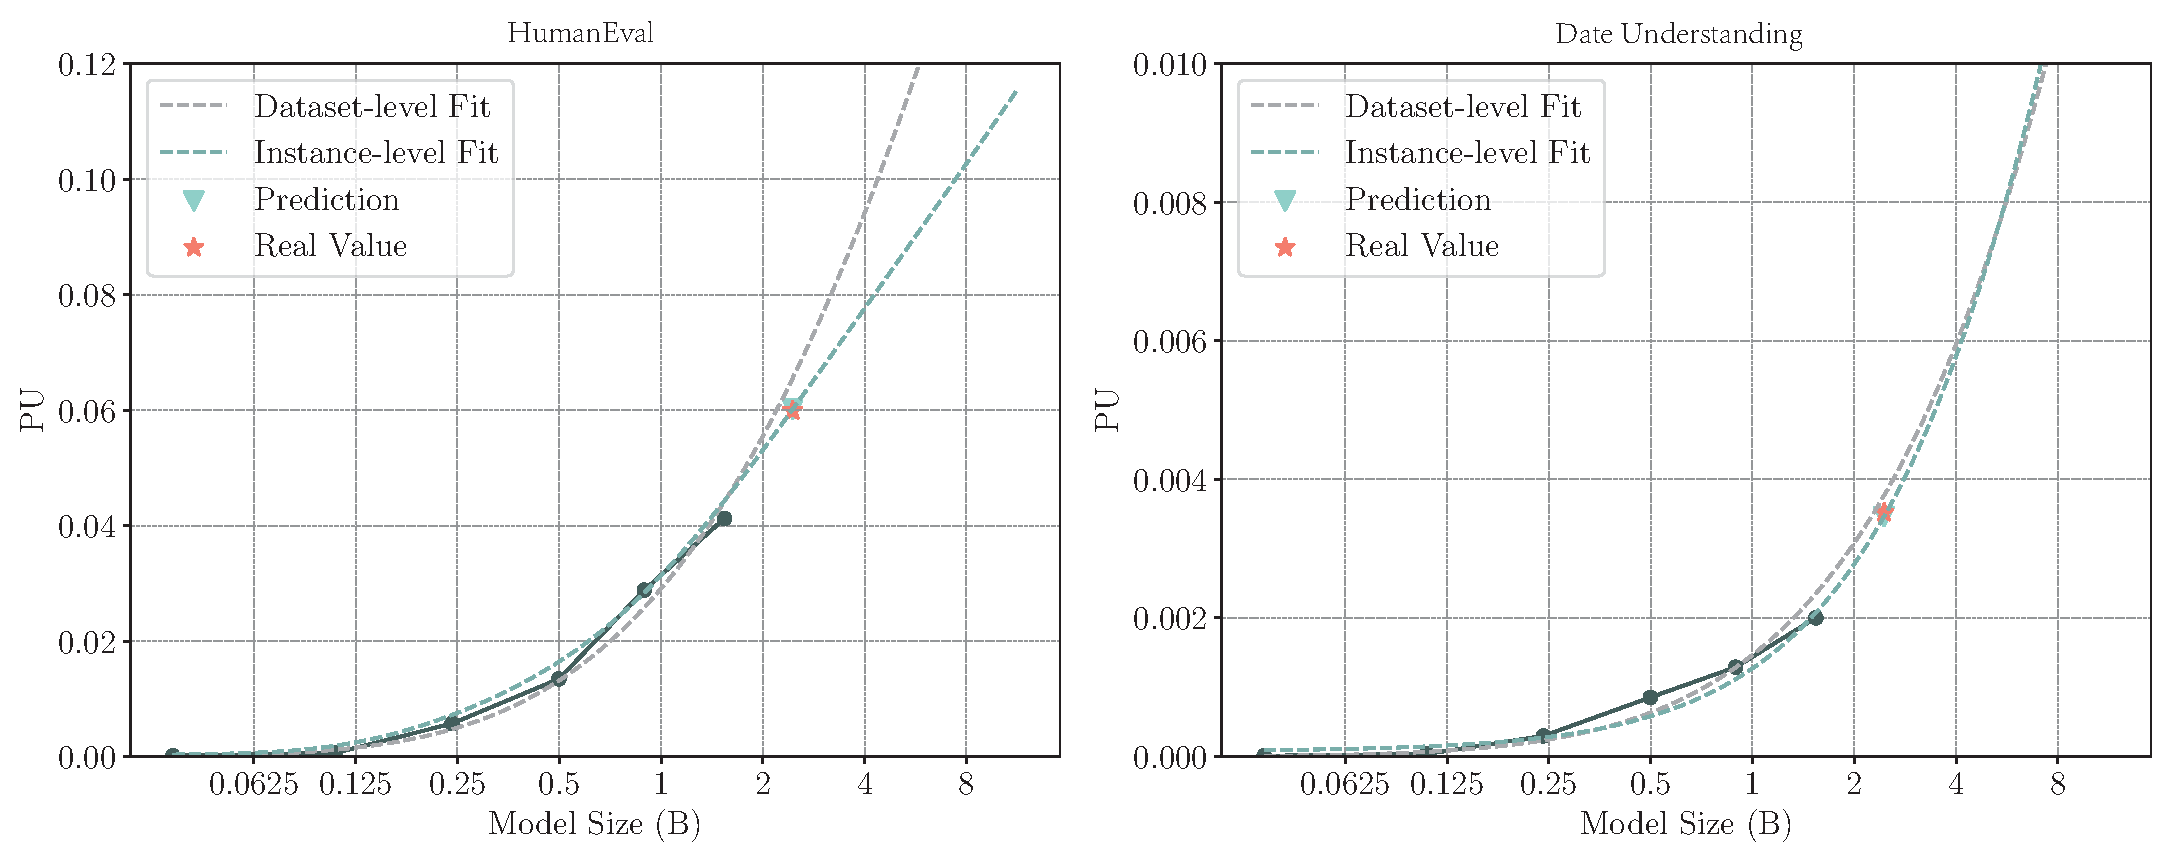
\includegraphics[width=1.02\linewidth]{pufigs/final_predict_2_set.pdf}
    \caption{本文成功预测了24亿参数模型的性能,(左图结果)偏差为0.05\% ,(右图结果)偏差为1.7\% 。 }
    \label{fig:final_curve_humaneval_series1} 
\end{figure}


\section{分析}
\label{sec:emergent}

{基于对任务性能可预测性的发现,我进一步对更广泛任务的扩展行为进行定量分析。我证明,即使有 “PassUntil” 带来的精细分辨率以及其他涌现能力的可预测性,仍有某些能力难以预测。本节给出它们的数学定义,并探讨这种扩展行为可能的解释。}
\begin{figure}
    \centering
        \centering
        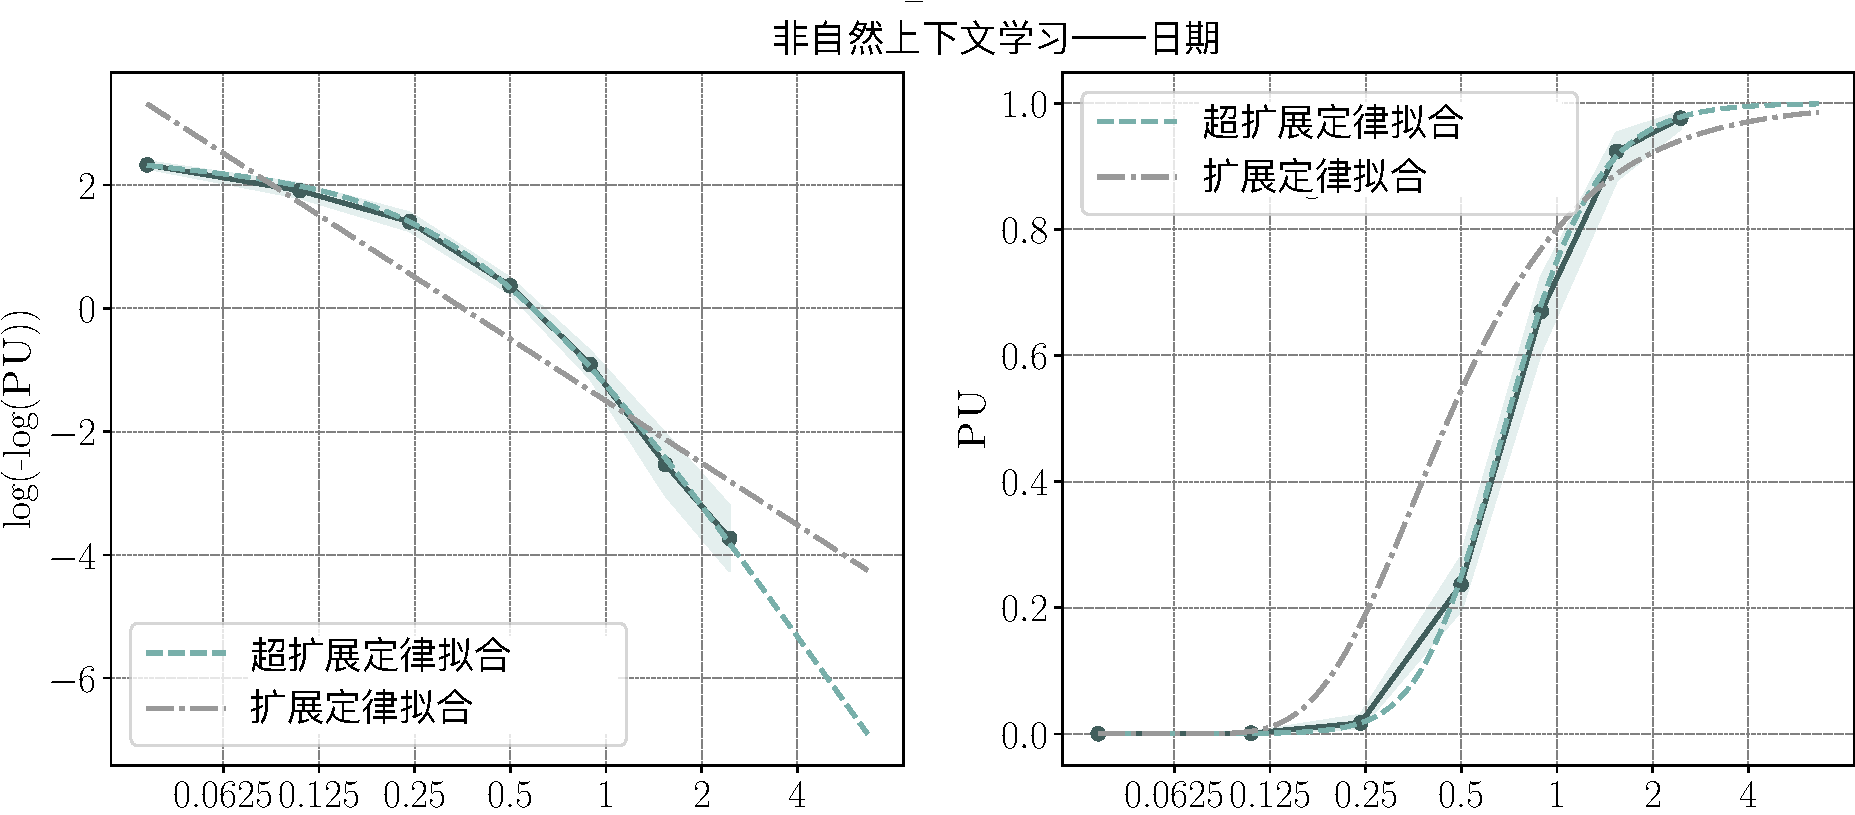
\includegraphics[width=1\linewidth]{pufigs/passrate_vs_modelsize_Dates_circuitfit.py.pdf}
        \centering
\end{figure}
\begin{figure}
        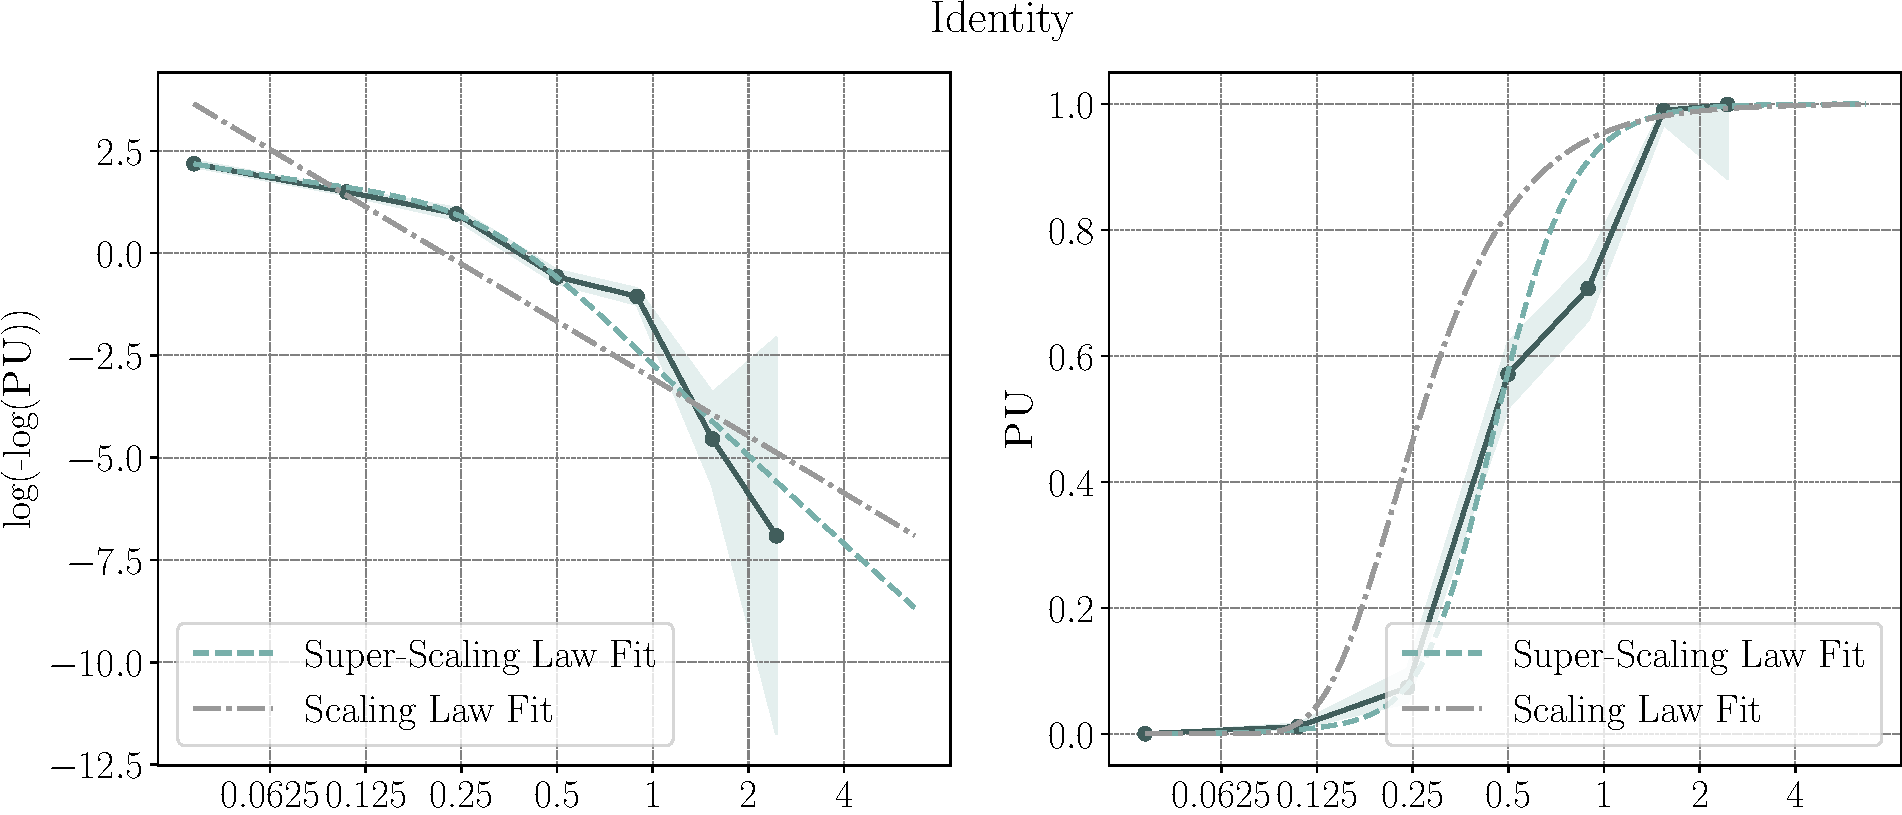
\includegraphics[width=1\linewidth]{pufigs/passrate_vs_modelsize_identity_circuitfit.py.pdf}
        \caption{{“日期”(Dates)和“原样输出”(Identity)任务的扩展曲线。在 $\operatorname{log}(-\operatorname{log}(\textsc{PU}))$ 与 $\operatorname{log}N$ 之间观察到凹函数关系。扩展定律拟合曲线为 {\color[rgb]{0.55, 0.6, 0.6}灰色},超扩展定律拟合曲线为 {\color[rgb]{0.3, 0.6, 0.45}绿色}。}}
        \label{fig:unnatural}
\end{figure}
\begin{figure}å
    \centering
    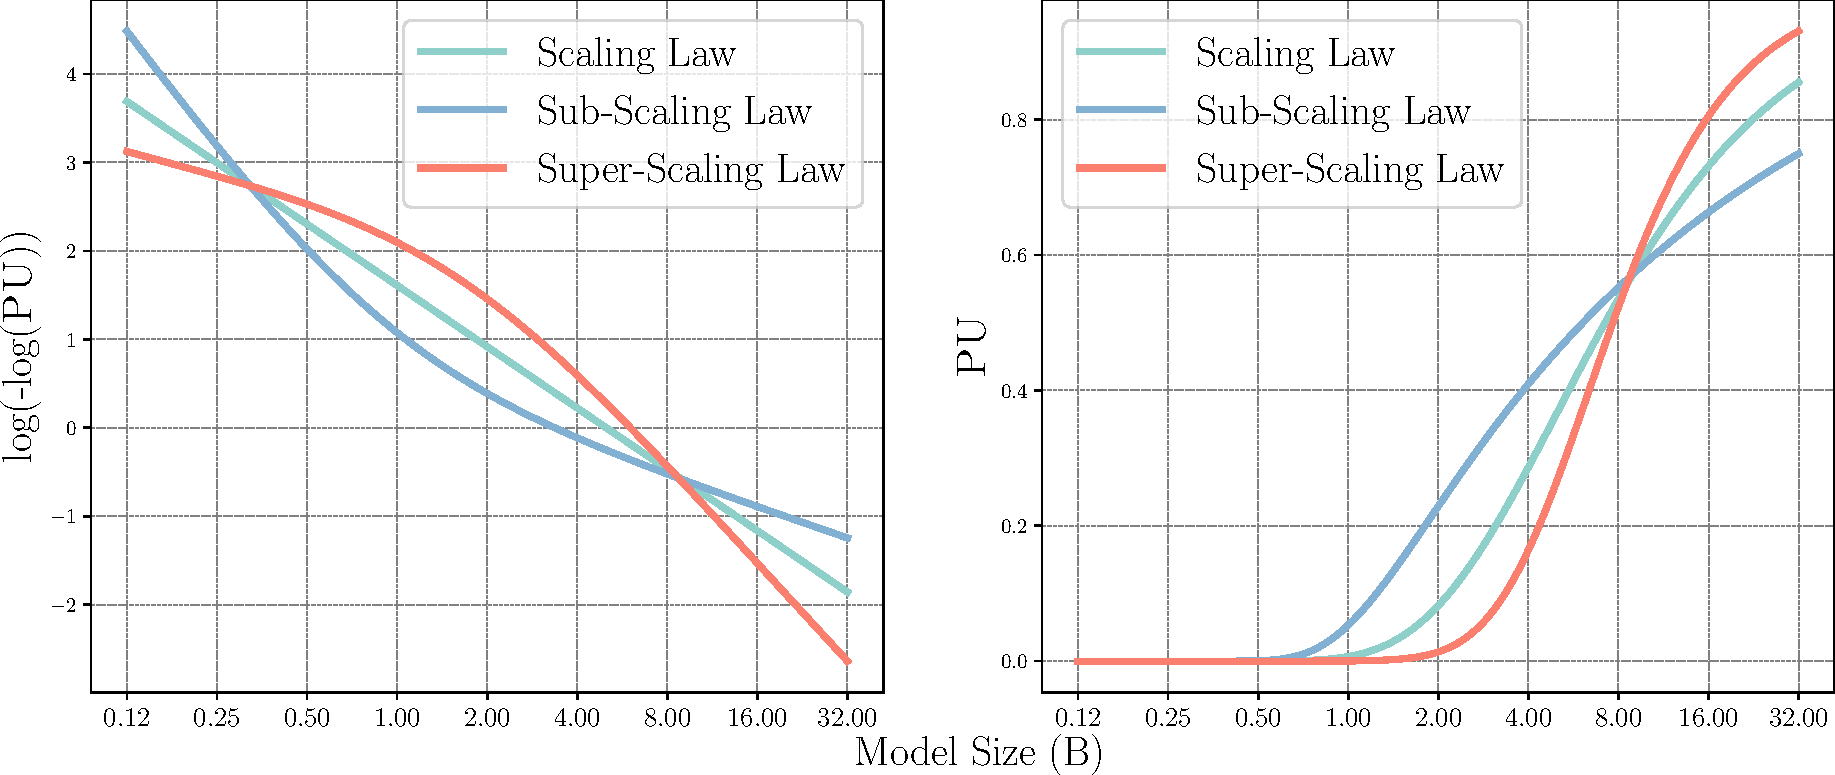
\includegraphics[width=1\linewidth]{pufigs/three_scaling_func.pdf}
    \caption{三种基本的扩展曲线类型,对应于 $\log(-\log(\textsc{PU}))$ 与 $\log N$ 之间的凸函数、线性函数和凹函数。}
    \label{fig:threekindsofgrowth}
\end{figure}

我研究了BigBench\citep{srivastava2022beyond} 中 “非自然上下文学习(UICL)” 类别的扩展曲线。“非自然上下文学习” 包含8个任务,专门用于研究上下文学习能力。这些任务涉及的输入 - 输出对经过有意调整,偏离了典型的训练分布,因此要求模型关注非传统的上下文模式。任务细节和示例见章节\ref{app:unantural_in_context_learning}。在拟合扩展曲线时,仅使用数据集层面的 “PassUntil”,因为这些测试实例是为测试大语言模型的一项技能而人工构建的,可能不存在难度变化。由于测试集较小,我从20个问题的测试结果中进行100次自助采样,并使用自助采样结果计算每个 “PassUntil” 估计值的标准误差(在图中以绿色显示)。 

此外,我展示了非自然上下文学习任务中其余固定子任务的扩展曲线。值得注意的是,图(a)、(b)和(c)中的曲线呈现出凹形模式,即\(\log(\log(-F(N))\)与\(\log N\)之间的关系。具体而言,“两位数”任务呈现出一种有趣的反向扩展趋势,这表明需要进一步研究以明确更清晰的趋势。

{
关于图(d)和(e)中的任务,我观察到这些任务对较小的模型构成重大挑战。具体来说,参数为3000万和1亿的模型未能实现非零通过率,这使得拟合分析的意义不大。此外,对于“反转成自然内容”任务,存在一种明显但轻微的次扩展定律增长趋势。这种趋势可能归因于该任务内在的多步骤特性。
}

\begin{figure}[!htbp]
        \centering
        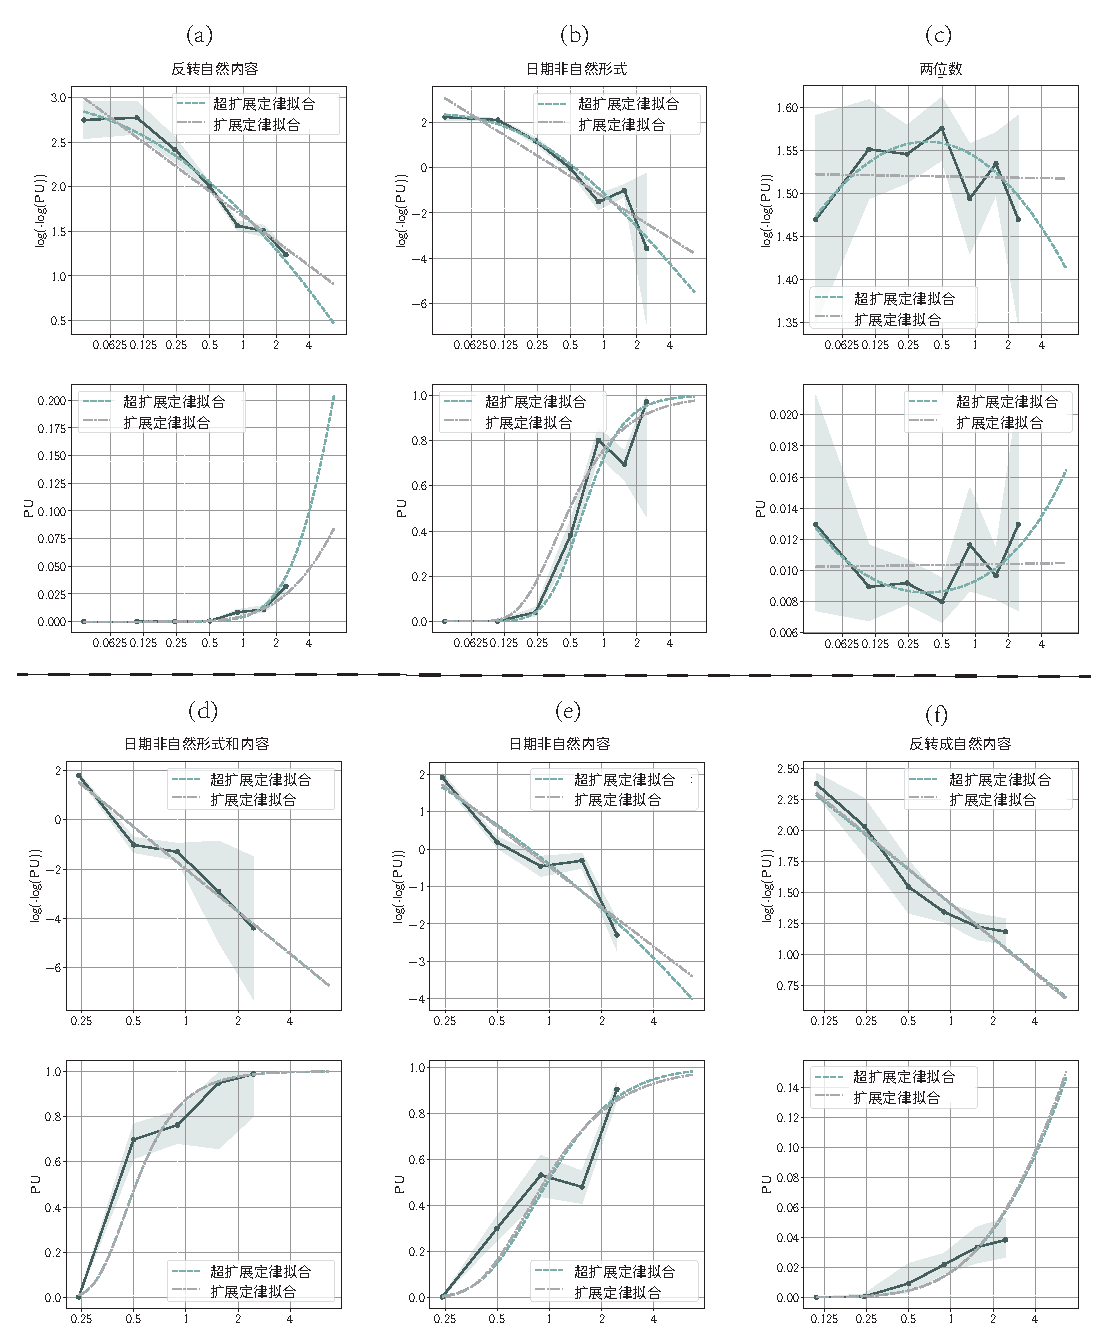
\includegraphics[width=0.9\linewidth]{pufigs/appendix_graph.pdf}
    \caption{{关于非自然上下文学习的补充图。灰色线表示扩展定律拟合,绿色线表示超扩展定律拟合。}}
    \label{fig:appendix_unnatural}
\end{figure}

\subsection{涌现现象的分类}
“日期”(Dates)和“原样输出”(Identity)任务的评估结果如图\ref{fig:unnatural}所示。其他任务见图\ref{fig:appendix_unnatural}。“日期”任务从参数规模3000万开始就呈现出非常平滑且持续的性能提升,而其他任务的提升则略显曲折。尽管如此,这些上下文学习任务中有5/8在\(\log(-\log(\textsc{PU}))\)与\(\log N\)之间呈现出严格的凹函数关系。另外3/8的任务由于对于3000万和1亿参数的模型来说难度极高,缺失了1或2个有效的估计点,因为即使采样\(10^5\)次,“PassUntil”分数仍为0,这留待未来进一步探索。这5/8的任务偏离了扩展定律(公式(\ref{eq:task_scaling_raw})),该定律要求此函数为线性。这意味着,与那些遵循任务扩展定律的任务不同。在遵循任务扩展定律的任务中,“增长速度”\(\alpha\)在不同模型规模下是一致的,而还存在一些任务,随着模型规模增大,其“增长速度”\(\alpha\)会增加。这种现象就是加速涌现现象的例证。为了具体讨论加速涌现现象,先给出任务扩展曲线的分类。

\subsection{涌现现象的数学定义}
由于公式(\ref{eq:loss_scaling_law})的损失扩展定律是模型扩展过程中唯一被广泛接受的原则,本文依据由它推导出来的公式(\ref{eq:task_scaling_raw})的任务扩展定律,来区分涌现现象和其他扩展行为。

% \newtheorem{definition}{定义}

对于一系列模型,设非嵌入参数的数量为变量\(N\),假设在某一任务上通过“PassUntil”估计得到的\(\textsc{PU}(N)\)是\(N\)的连续函数。定义\(F(N) = \operatorname{log}(-\operatorname{log}(\textsc{PU}(N)))\),{那么一个任务的扩展曲线可分为三个基本主要类别\footnote{如果\(F(N)\)同时有凸函数和凹函数部分,那么可称其为混合增长。}:}
\begin{enumerate}
    \item 如果\(F(N)\)是\(\operatorname{log}N\)的线性函数,那么该任务遵循扩展定律增长。
    \item 如果\(F(N)\)是\(\operatorname{log}N\)的凸函数,那么该任务遵循次扩展定律增长。
    \item 如果\(F(N)\)是\(\operatorname{log}N\)的凹函数,那么该任务遵循超扩展定律增长,即“加速涌现”。
\end{enumerate}


图\ref{fig:threekindsofgrowth}展示了这三种增长类型的可视化结果。定性地看,当性能开始显著提升时,这三种类型的扩展曲线都类似于指数增长。然而,它们在性质上是不同的。遵循任务扩展定律增长或次扩展定律增长的任务扩展曲线更容易预测和控制,而加速涌现则不易预测,并且随着模型规模增大可能会失控。

{\textbf{扩展曲线形状的成因}。上述数学定义为本文提供了检验关于这些扩展行为成因假设的机会。在此,我首先研究以下假设:涌现能力可能由多步推理引发\citep{srivastava2022beyond, wei2022emergent, schaeffer2023emergent}。}

我证明了\textbf{”多步推理会导致次扩展定律增长”}。

\begin{theorem}
假设每个推理步骤的成功率(通过“PassUntil”衡量)遵循扩展定律增长,那么多步推理的成功率遵循次扩展定律增长。
\end{theorem}


    
\begin{proof}
    假设推理步骤\(i\)的“PassUntil”分数(\(\textsc{PU}\))遵循具有系数\(c_i\)和\(\alpha_i\)的扩展定律增长,总体成功率为:
    \begin{equation}
    \begin{split}
     F(N) & = \operatorname{log}\left(-\operatorname{log}\prod_i P_i\right)\\ & = \operatorname{log}\left(-\operatorname{log} \prod_i\operatorname{exp}\left(- c_i \operatorname{exp}(-\alpha_i \operatorname{log} N)\right)\right) \\ & = \operatorname{log}\left(\sum_i c_i \operatorname{exp}\left(-\alpha_i \operatorname{log} N \right)\right)\\
    \end{split}
    \end{equation}
    然后对\(F(N)\)关于\(\log N\)求二阶导数,可得:
    \begin{equation}
    \label{eq:app_th_1}
    \begin{split}
        \frac{\partial^2{F}}{\partial{(\operatorname{log}N )^2}} & = \frac{\sum_i \alpha_i^2 c_i \exp(-\alpha_i \log N) \sum_i c_i \exp(-\alpha_i \log N)}{(\sum_i c_i\exp(-\alpha_i \log N))^2} \\
    & - \frac{(\sum_i \alpha_i c_i \exp(-\alpha_i \log N) )^2}{(\sum_i c_i\exp(-\alpha_i \log N))^2}
    \end{split}
    \end{equation}
    令\(k_i = c_i \exp(-\alpha_i \log N) > 0\),式(\ref{eq:app_th_1})变为:
    \begin{equation}
    \frac{\sum_i \alpha_i^2 k_i\sum_i k_i - (\sum_i \alpha_i k_i)^2}{(\sum_i k_i)^2}
    \end{equation}
    利用柯西 - 施瓦茨不等式,可以证明:
    \begin{align}
    \frac{\partial^2{F}}{\partial{(\operatorname{log}N )^2}} \geq 0, \quad \forall  \alpha_i > 0, c_i > 0
    \end{align}
    只有当\(\frac{\alpha_i \sqrt{k_i}}{\sqrt{k_i}} = \text{常数}\)时,等式成立,即推理链中的所有步骤以相同速度扩展时。
    因此,\(F(N)\)是\(\operatorname{log}N\)的凸函数,且扩展曲线呈现次扩展定律增长。 
\end{proof}


这个证明也可以更直观地理解:增长速度最初会受到那些简单步骤改进的推动,最终会受到最困难步骤的限制,从而呈现出增长速度下降的趋势。

我提出另一种假设:根据\citet{elhage2021mathematical},大语言模型中可能存在多个神经“回路”,只要其中一个回路能够成功解决测试实例,就认为该测试实例通过。这个假设的灵感来自于\cite{varma2023explaining}对“顿悟”现象的解释。他们提出在Transformer内部存在一个记忆回路和一个泛化回路,“顿悟”现象是由于在训练过程中泛化回路比记忆回路效率更高所导致的。我将证明,基于这个假设,扩展曲线会呈现出涌现的特征。

\begin{theorem}
假设大语言模型中存在多个负责解决任务的回路\(i\),每个回路都呈现扩展定律增长且有\(\textsc{PU}_i\)。{并且假设}任务的成功率是这些回路的多数表决结果,即\(F(N)  = \operatorname{log}\left(-\operatorname{log}\max_i \textsc{PU}_i\right)\)。
那么,\(F(N)\)是\(\operatorname{log}N\)的凹函数。
\end{theorem}

\begin{proof}
    \begin{equation}
    \label{eq:app_th_2}
    \begin{split}
    F(N) &= \operatorname{log}\left(-\operatorname{log}\max_i \operatorname{exp}\left(- c_i \operatorname{exp}(-\alpha_i \operatorname{log} N)\right)\right) \\
        &= \operatorname{log} \min_i  c_i \operatorname{exp}(-\alpha_i \operatorname{log} N) \\
    &=  \min_i (\operatorname{log} c_i-\alpha_i \operatorname{log} N) \\
    \end{split}
    \end{equation}
    由于取最小值操作保持凹性,所以\(F(N)\)是\(\operatorname{log}N\)的凹函数。 
\end{proof}


我通过拟合UICL任务的扩展曲线对该假设进行了初步检验。在实际操作中,与\cite{varma2023explaining}类似,我采用了一种软多数表决版本。我在两个回路之间应用加权组合。并且假设回路数量为\(2\)。因此,用\({w_1}({\alpha_1}\log N-\log{c_1}) + {w_2}({\alpha_2}\log N - \log c_2)\)来拟合\(F(N)\),其中\(w_1\)和\(w_2\)由\({\alpha_i}\log N -\log {c_i}\)的Softmax函数给出。得到的拟合曲线在图\ref{fig:unnatural}和图\ref{fig:appendix_unnatural}中以{\color[rgb]{0.3, 0.6, 0.45}绿色}线条展示。可以看到,这个假设得到的拟合曲线与观察到的性能扩展曲线更为吻合。 



\section{本章小结}

本章引入了一种全新的评估策略,该策略能够检测模型在规模缩放过程中极其微小的性能提升,从而为定量衡量任务扩展定律和涌现能力开辟了道路。借助这种方法,我成功预测了更大规模模型的任务性能。此外,对涌现能力进行了定量分析,从而更清晰地洞察扩展过程中不可预测因素的本质和起源。这项研究不仅加深了我对大语言模型(LLMs)缩放特性的理解,也为未来大语言模型可预测的规模化扩展研究奠定了基础。 
\chapter{可预测预训练技术应用--MiniCPM-2B}

\section{基于WSD调度器的多阶段训练策略}
\label{sec:trainingstrategy}
通常,遵循指令的大语言模型(LLMs)的训练包含预训练阶段和监督微调(SFT)阶段~\citep{zhang2023instruction,wei2021finetuned}。在预训练阶段,数据由大规模无标签数据组成,而在监督微调阶段,高质量的有标签数据成为优化目标。

鉴于在WSD学习率调度器的衰减阶段观察到的显著损失下降,我们假设在此阶段整合高质量的有标签数据具有双重优势:
\begin{itemize}
    \item 除了在监督微调阶段,在退火阶段引入此类数据有助于模型进行更全面的学习。具体而言,相较于预训练数据分布,它能促使模型在针对监督微调数据分布时实现更显著的损失降低。这种方式与实际用户场景更为契合。
    \item 与在整个预训练过程中均匀分布高质量数据不同,此方法通过集中处理数据并维持持续预训练来提升训练效果。如果我们不预先确定训练步数,在持续的预训练过程中重复使用小数据集可能会产生负面影响。
\end{itemize}

基于这两个假设,我们提出以下训练策略:在预训练阶段,仅使用大规模的粗质量预训练数据,这类数据丰富,且在提供更多计算资源时能够支持持续训练。在退火阶段,我们使用多样且高质量的、面向知识与能力的监督微调数据,并将其混入预训练数据中。

为验证我们训练策略的优势,我们使用(A) MiniCPM - 2.4B稳定阶段的中间检查点和(B) MiniCPM - 1.2B稳定阶段的最后检查点进行对比实验。具体来说,我们比较以下几种情况:

\begin{enumerate}
    \item A - 1:24亿参数模型,仅使用预训练数据进行衰减,随后进行40亿词元的监督微调。
    \item A - 2:24亿参数模型,使用上述混入预训练数据中的高质量无标签数据和监督微调数据进行衰减,随后也进行40亿词元的监督微调。
    \item B - 1:12亿参数模型,仅使用预训练数据进行衰减,随后进行60亿词元的监督微调。
    \item B - 2:12亿参数模型,仅使用预训练数据进行衰减,随后进行120亿词元的监督微调。
    \item B - 3:12亿参数模型,使用上述混入预训练数据中的高质量数据 + 监督微调数据进行退火,随后也进行60亿词元的监督微调。 
\end{enumerate}

实验结果如表\ref{tab:dataexperiments}所示。我们可以看到,尽管A - 2和A - 1经历了相同的监督微调数据分布,但在衰减阶段添加监督微调数据提升了模型表现。B - 2和B - 3的比较表明,仅进行监督微调的不足并非源于监督微调阶段训练词元不足。 

\begin{table}[h]
\centering
\begin{tabular}{lccccccc}
\toprule
            & \textbf{C - Eval} & \textbf{CMMLU} & \textbf{MMLU} & \textbf{GSM8K} & \textbf{MATH} & \textbf{HumanEval} & \textbf{MBPP} \\ \midrule
A - 1 & 40.0  & 41.5  & 44.6 & 27.7  & 5.1  & 27.7      & 24.4 \\
A - 2 & \textbf{52.6}  & \textbf{51.1} & \textbf{50.9} & \textbf{42.3 } & \textbf{5.4}  & \textbf{30.4 }     & \textbf{30.3} \\
\midrule

B - 1 &   40.9  & 41.5 & 47.9 &  34.2 & 7.9   &  43.9 & 30.5 \\
B - 2 &  41.2 &  42.0 &    47.9  & \textbf{34.4} & 7.3 &  43.9 & 29.8  \\ 
B - 3 & \textbf{49.1}  & \textbf{46.8}  & \textbf{49.6} & 31.8  & \textbf{10.5}  & \textbf{44.5}  & \textbf{32.8}\\
% B - 4 & 43.9 & 45.3 &  50.1 & 39.3 & 10.1 & 45.1 & 33.5 \\
\bottomrule
\end{tabular}
\caption{不同训练策略的消融研究。
}
\label{tab:dataexperiments}
\end{table}

结果表明,在衰减阶段开始时引入高质量数据的益处远高于仅在监督微调阶段添加。因此,我们建议模型能力的专业化和增强应从衰减阶段开始。 

\section{MiniCPM系列}


在本节中,我们将介绍MiniCPM,这是一系列小语言模型,主要基于两个模型构建,分别具有24亿和12亿非嵌入参数,在各自的20亿和10亿规模类别中表现卓越。MiniCPM还展现出与70亿 - 130亿参数规模的语言模型相当的能力,如Llama2 - 7B~\citep{touvron2023llama}、Mistral - 7B~\citep{jiang2023mistral}、Gemma - 7B~\citep{Banks2024Gemma}以及Llama - 13B~\citep{touvron2023llama}等。尽管模型规模较小,但我们精心设计了训练方法,以便在模型规模和数据范围上实现无缝扩展。这在我们的模型风洞实验中得到了体现,其中包括全面的超参数优化(第\ref{MWTE}节),以及采用WSD(预热 - 稳定 - 衰减)学习率调度器(第\ref{sec:wsdlrs}节)。后者专为在预训练token数量未预先定义的情况下进行连续训练而设计,使得模型中间检查点的重用极具可行性。我们对MiniCPM的训练动态进行了详细分析,结果表明WSD调度器展现了模型预训练中有趣的损失景观。借助WSD调度器,我们现在还能够以在模型轴上的线性工作量和在数据轴上的可忽略工作量来研究数据 - 模型缩放定律,而传统方法在考虑模型和数据轴的缩放时需要二次工作量。缩放定律的结果表明,与Chinchilla最优缩放相比,其数据大小与模型大小的比率要高得多~\citep{hoffmann2022training}。

此外,我们还介绍了MiniCPM家族,包括MiniCPM - DPO、MiniCPM - 128K和MiniCPM - MoE。我们针对既定基准对MiniCPM家族进行了评估,彰显了它们作为小语言模型令人瞩目的能力:(1)基础模型超越了Mistral - 7B和LLama - 13B。(2)DPO模型在MTBench~\citep{zheng2024judging}上超越了zephyr - 7B~\citep{tunstall2023zephyr}。(3)24亿参数的MiniCPM - 128K模型的性能超越或与Yarn - Mistral - 7B - 128K~\citep{peng2023yarn}和ChatGLM3 - 6B - 128K~\citep{du2021glm}等模型相当。(4)具有40亿激活参数的MiniCPM - MoE与Llama2 - 34B~\citep{touvron2023llama}不相上下。

总之,MiniCPM开启了小语言模型发展的新阶段,例证了小语言模型的潜在能力,并倡导以更科学、可持续的方式扩大大语言模型的规模。 



\section{模型基本配置}
在本节中,我们开始介绍融合了上述观察结果与技术的MiniCPM模型。
\label{sec:model}
\begin{table}[htbp]
    \centering
\scalebox{0.90}{
    \begin{tabular}{l|ccccccccc}
    \toprule
        模型 & N(十亿)& $d_m$ & $d_{ff}$ & $d_h$ & $n_q$ & $n_{kv}$ & $L$ & 批量大小(百万) & 词元数(T)\\
    \midrule
       MiniCPM - 1.2B & 1,247,442,432  & 1,536 & 3,840 & 64 & 24 & 8 & 52 & 200万 $\rightarrow$ 400万 & 1.1T\\
       MiniCPM - 2.4B & 2,442,057,984 & 2,304 & 5,760 & 64 & 36 & 36 & 40 & 400万 &  1.1T\\
    \bottomrule
    \end{tabular}
}
    \caption{MiniCPM的模型配置。N(十亿)、$d_m$、$d_{ff}$、$d_h$、$n_q$、$n_{kv}$、$L$、批量大小(百万)、词元数(T)分别代表模型的非嵌入参数数量、模型隐藏维度、前馈层瓶颈维度、注意力头维度、查询数量、键/值数量、层数、训练批量大小、总训练词元数。}
    \label{tab:model_configs}
\end{table}

\section{词表}
尽管MiniCPM的参数规模较小,但其目标是对多样的数据分布进行建模,在中英文方面表现出色。因此,我们的词表相对较大。对于24亿参数的模型,我们使用了由122,753个词元组成的分词器(记为MiniCPMTokenizer - 120K)。这个词表是从广泛多样的语言数据中构建而成,利用sentencepiece库\footnote{\url{https://github.com/google/sentencepiece}}进行字节对编码(BPE)~\citep{sennrich-etal-2016-neural},并且包含了诸如繁体字、生僻字、表情符号以及希腊字母、西里尔字母等特殊符号。

对于小语言模型(SLM)而言,如果词表较大,嵌入参数会占用大量的参数空间。因此,对于我们12亿参数的模型,我们使用了一个更小的词表MiniCPMTokenizer - 70K。与MiniCPMTokenizer - 120K分词器相比,我们在相同文档上重新训练了分词,同时将最大词表数量设置为64,000。对于特殊字符,我们仅添加了繁体字、表情符号和特殊符号,但省略了中文生僻字。

我们对未包含在分词器训练集中的30万篇中文、英文、代码和学术论文文档进行了评估。MiniCPM - 120K分词器实现了最高的压缩率(字节/词元)。

\begin{table}[htbp]
    \centering
    \begin{tabular}{lccccc}
    \toprule
      & {\textbf{百川2}}  & {\textbf{ChatGLM2}} & {\textbf{Llama2}} & {\textbf{MiniCPM - 120K}}  & {\textbf{MiniCPM - 70K}}\\
    \midrule
    词表大小 & 125,696 & 64,794 & 32,000 & 122,753 & 73,440\\
    \midrule
    \multicolumn{6}{c}{\textbf{压缩率}(字节/词元) }\\
    \midrule
    中文 & 3.64   & 3.54  & 1.87  & \textbf{3.73} &  3.56 \\
    英文 & 4.12   & 4.02  & 3.78  & \textbf{4.14} & 4.02 \\
    代码    & 2.71   & 2.71  & 2.74  & \textbf{2.81} & 2.76 \\
    论文   & 2.74   & 2.88  & \textbf{2.97}  & 2.93 & 2.88\\
    \midrule
    平均 & 3.30   & 3.29  & 2.84  & \textbf{3.40}  & 3.31 \\
    \bottomrule
    \end{tabular}
    \caption{压缩率对比。}
    \label{tab:compression_ratio}
\end{table}
    

\section{模型细节}
\subsubsection{模型细节}
\noindent\textbf{词表}:对于MiniCPM - 2.4B,我们使用词表大小为122,753的分词器;对于MiniCPM - 1.2B,使用词表大小为73,440的分词器。12亿参数模型采用较小词表有助于提升效率,且不会过多损害性能。分词器的详细信息见附录\ref{app:tokenizer}。包含嵌入参数后,总参数分别增加了3亿和2亿。 

\noindent\textbf{共享输入 - 输出层}:对于小语言模型(SLM),嵌入会占用较大的参数空间。为减小模型参数规模,MiniCPM - 2.4B和MiniCPM - 1.2B都采用了嵌入共享技术。 
% 对于24亿参数模型,得到的嵌入参数为$2304 \times 122753 = 0.28B$;对于12亿参数模型,约为$1536 \times  \sim 0.11B$。 

\noindent\textbf{深而窄的网络}:在训练MiniCPM - 1.2B之前,我们先训练了MiniCPM - 2.4B。与Phi - 2~\citep{Javaheripi2023Phi2}相比,训练MiniCPM - 2.4B时,我们采用了更深且更窄的架构(40层,而Phi - 2为32层)。最近,~\cite{liu2024mobilellm}提出为小语言模型训练深而窄的网络,这与我们的观点一致。因此,对于MiniCPM - 1.2B,我们进一步加深并收窄了其架构。 

\noindent\textbf{组查询注意力}:我们在训练MiniCPM - 2.4B时,对注意力层未做修改。而受~\cite{liu2024mobilellm}启发,我们在MiniCPM - 1.2B中应用了组查询注意力(Group Query Attention)~\citep{ainslie-etal-2023-gqa},以进一步减少参数数量。

\section{训练阶段}
MiniCPM基础模型的整体训练包括三个阶段:稳定训练阶段、衰减阶段、监督微调(SFT)阶段~\citep{zhang2023instruction,wei2021finetuned}。在整个训练过程中,我们使用Adam优化器~\citep{kingma2014adam}。 

\textbf{稳定训练阶段}:我们使用了约1万亿的数据(数据分布见\ref{fig:appdatamixture}节),其中大部分数据来自公开数据集。我们采用在模型风洞实验中发现的最优配置,即WSD学习率调度器(WSD LRS),批量大小为393万,最大学习率为0.01。

\textbf{衰减阶段}:我们使用预训练数据和高质量监督微调(SFT)数据的混合数据。
对于WSD调度器的具体退火形式,我们采用指数退火,即$f(s - T)=  0.5^{(s - S)/T}$,其中$T$设置为5000步(200亿词元)。

\textbf{监督微调(SFT)阶段}:我们发现仍然有必要进行单独的监督微调阶段。我们使用与退火阶段类似的监督微调数据,但不包含预训练数据,并使用约60亿词元进行训练。监督微调的学习率与退火结束时的学习率一致,并且也采用带有指数衰减的WSD调度器。 





\section{训练数据分布}
\label{sec:appdatadistrbution}

\begin{figure}[htbp]
    \centering
    \begin{minipage}{0.48\linewidth}
        \centering
        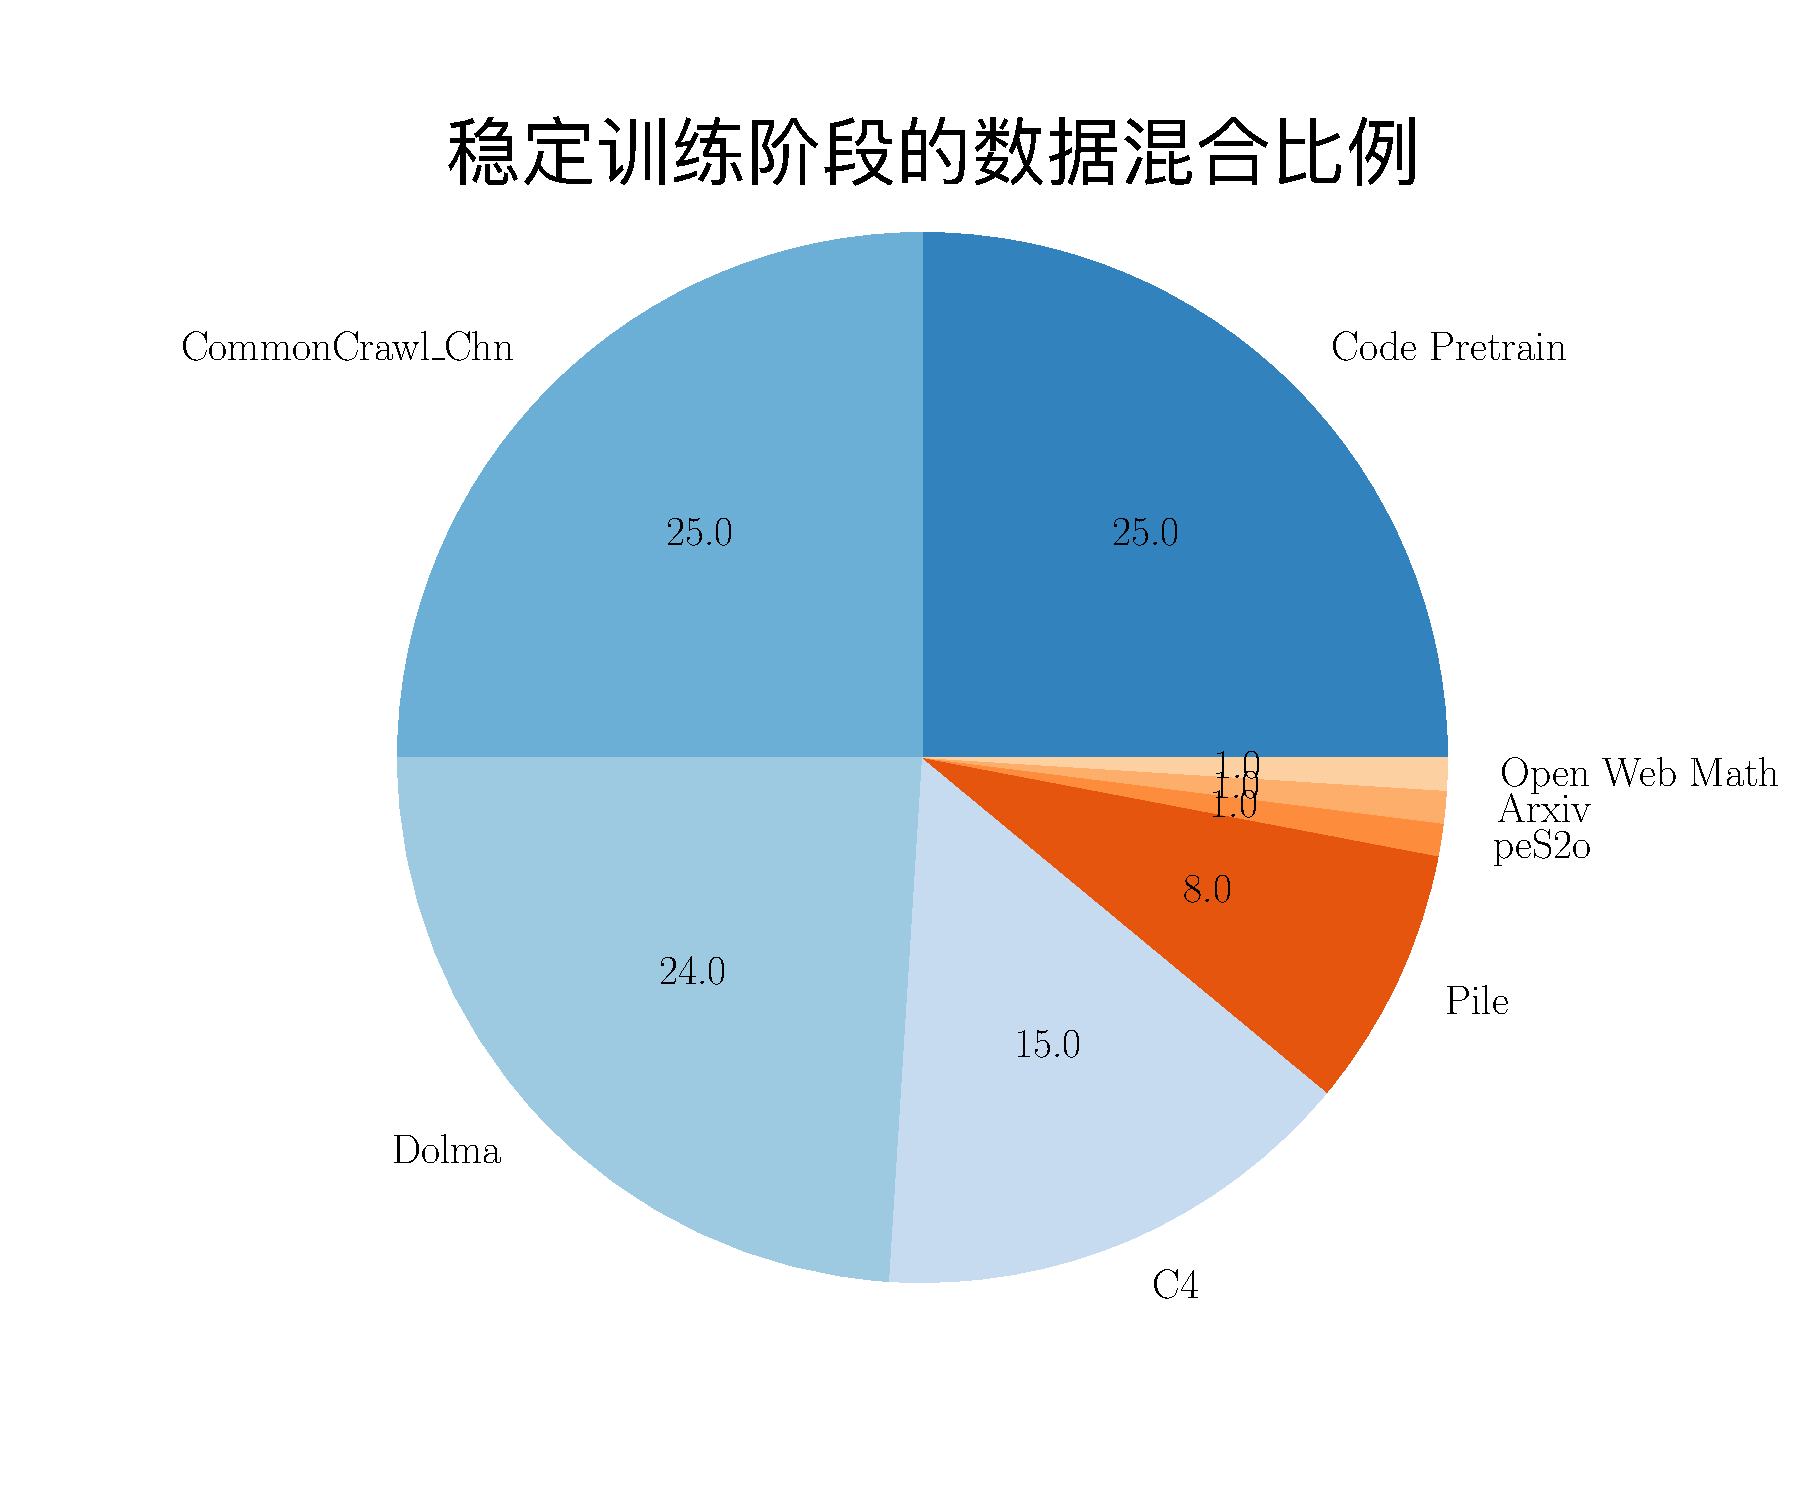
\includegraphics[width=1.0\linewidth]{minicpmFig/stable_mixture.pdf}
    \end{minipage}
    \hfill 
    \begin{minipage}{0.48\linewidth}
        \centering
        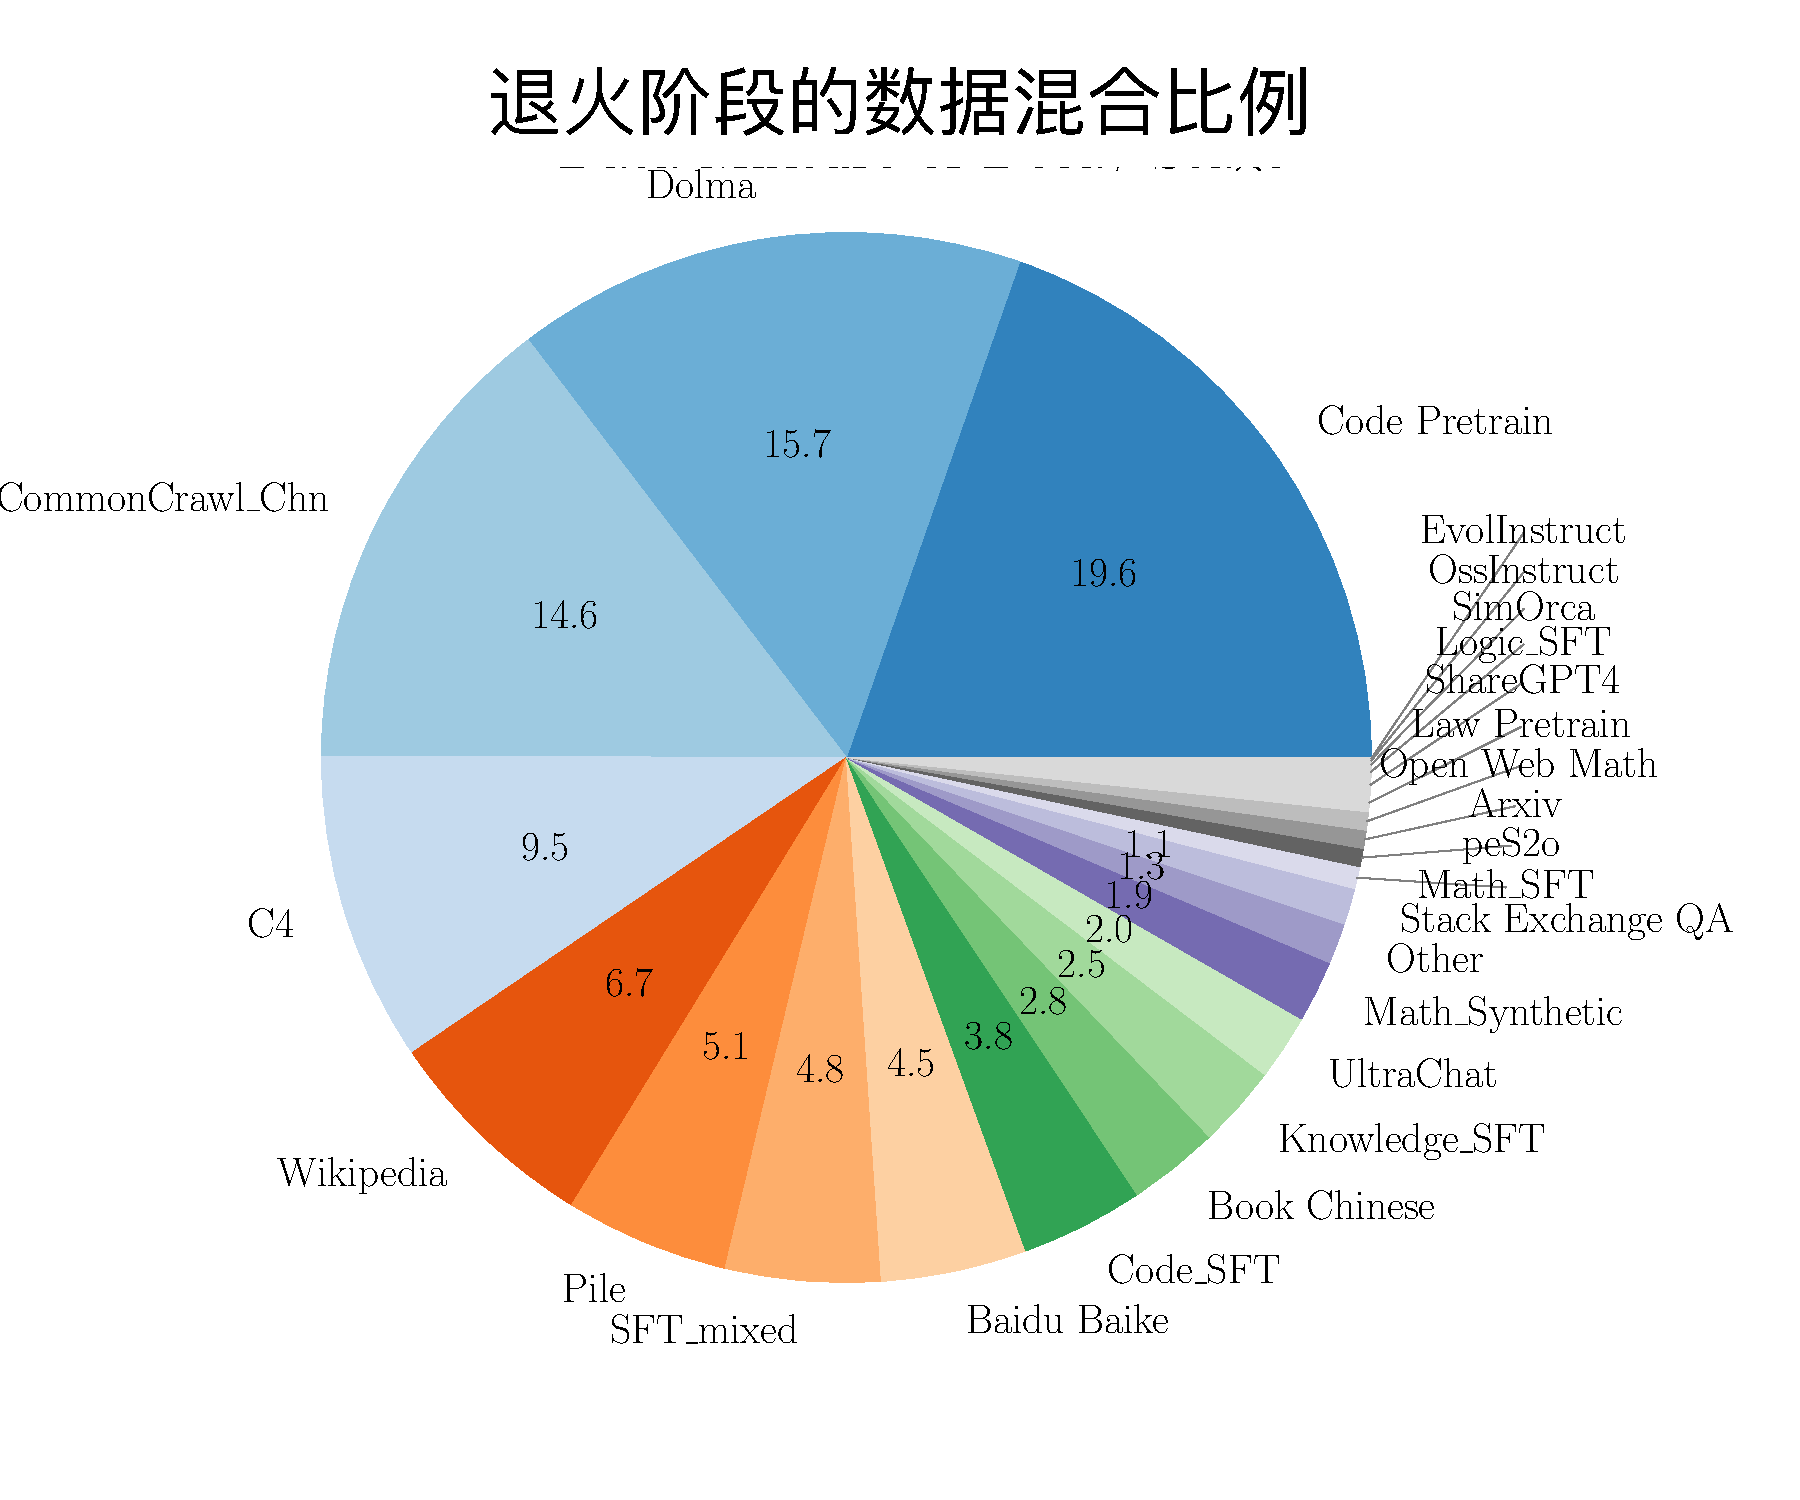
\includegraphics[width=1.0\linewidth]{minicpmFig/decay_data_mixture.pdf}
    \end{minipage}
    \caption{不同训练阶段的数据混合情况。左侧展示的是稳定阶段,右侧展示的是衰减阶段。}
        \label{fig:appdatamixture}
\end{figure}

我们在图\ref{fig:appdatamixture}中介绍训练数据的分布。在图中,CommonCrawl\_Chn是一个中文语料库,源自CommonCrawl原始语料库并经过了全面清理。Dolma~\citep{dolma}、C4~\citep{2019t5}和Pile~\citep{gao2020pile, biderman2022datasheet}是英文语料库。这些语料库内部以及相互之间都使用MinHash算法~\citep{broder1997resemblance}进行了去重。代码预训练数据包含stack~\citep{Kocetkov2022TheStack}和StarCoder~\cite{li2023starcoder},并进行了内部去重和交叉去重。在衰减阶段,混合数据包含更多样化的数据和专有数据,包括UltraChat~\citep{ding2023enhancing}、SlimOrca~\citep{SlimOrca, SlimOrcaDedup}、OssInstruct~\citep{wei2023magicoder}、EvolInstruct~\citep{xu2023wizardlm}。后缀为SFT的数据是我们的专有数据,包括力扣(LeetCode)题目、幼儿园到12年级(K12)的教科书及题目等。 

\subsubsection{训练损失}

\definecolor{darkgreen}{HTML}{476E6B}

在C4数据集上的整体训练损失如图\ref{fig:loss_c4}所示。我们可以看到,正如前期实验所预期的那样,损失在衰减阶段急剧下降。由于我们使用的是指数衰减,在学习率降至最大学习率的10\%以下后,损失仍在下降。然而,因为在衰减阶段之后我们会继续对模型进行监督微调(SFT),所以我们不会使用最终的检查点。我们进行微调所基于的检查点显示在\textcolor{darkgreen}{深绿色}线段的最后一个检查点处。MiniCPM - 1.2B中的首次损失下降是增大批量大小的结果,这可能与降低学习率有类似的效果~\citep{smith2017don}。

\definecolor{orange}{HTML}{FFA500}

\begin{figure}[htbp]
    % 第一个子图的minipage
        \centering
        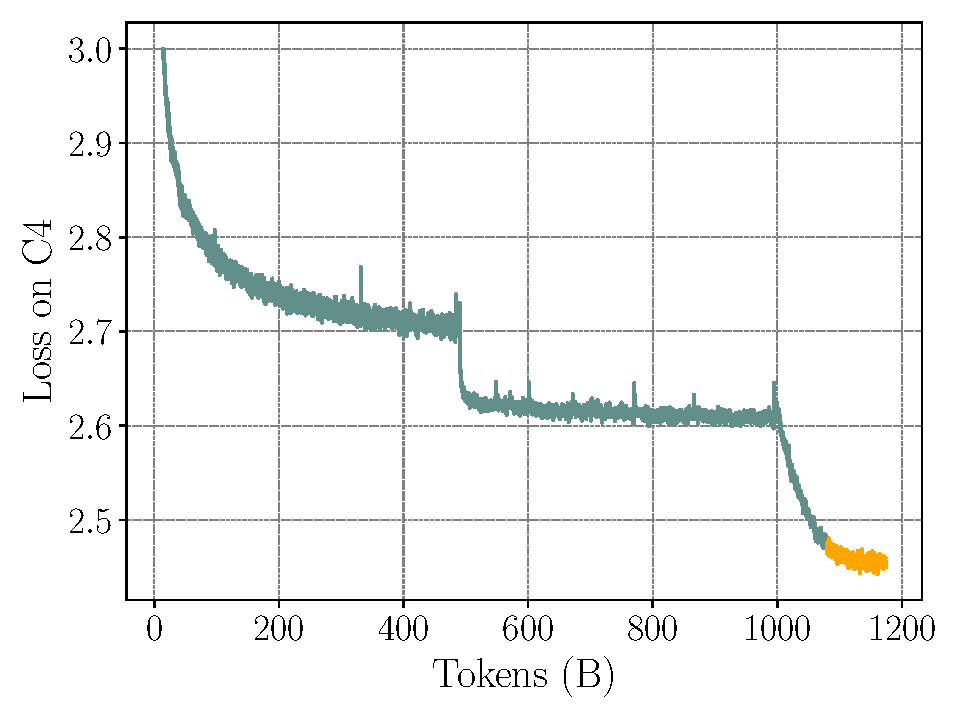
\includegraphics[width=0.9\linewidth]{minicpmFig/1.2B_c4_loss_smoothed.pdf}
    % 第二个子图的minipage
\end{figure}

\begin{figure}[htbp]
    \centering
    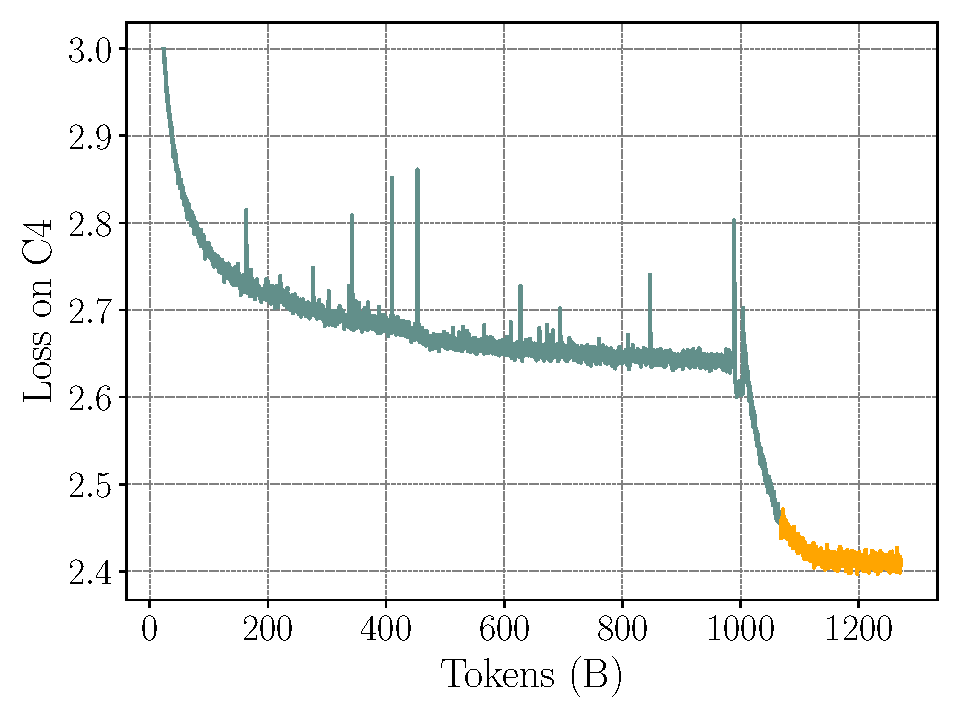
\includegraphics[width=0.9\linewidth]{minicpmFig/2.4B_c4_loss_smoothed.pdf}
    \caption{MiniCPM - 1.2B(左)和MiniCPM - 2.4B(右)在C4数据集上的损失曲线。损失曲线尾部的\textcolor{orange}{橙色}线段表示剩余的衰减过程,MiniCPM发布版本中未使用该部分。}
    \label{fig:loss_c4}
\end{figure}

\section{评估}
\label{sec:evaluation}
整体评估使用我们的开源工具UltraEval\footnote{https://ultraeval.openbmb.cn/home}。UltraEval是一个用于评估基础模型能力的开源框架。它提供了一个轻量级且用户友好的评估系统,支持对主流大模型的性能评估,满足模型训练团队的快速评估需求。其底层推理和加速使用开源框架vLLM~\citep{kwon2023efficient},数据集包括常用数据集:用于评估英语知识的MMLU~\citep{hendrycks2020measuring}、用于评估中文知识的CMMLU~\citep{li2024cmmlu}和C - Eval~\citep{huang2024c}、用于评估编程能力的HumanEval~\citep{chen2021evaluating}和MBPP~\citep{austin2021program}、用于评估数学能力的GSM8K~\citep{cobbe2021training}和MATH~\citep{hendrycks2021measuring}、用于评估常识推理能力的HellaSwag~\citep{zellers2019hellaswag}、ARC - e~\citep{clark2018think}、ARC - c~\citep{clark2018think}以及用于评估逻辑推理能力的BBH~\citep{suzgun2022challenging}。

由于对大模型进行标准化评估存在困难,且许多模型评估缺乏公开可用的提示词和测试代码,我们尽力调整评估方法以适用于各种模型类型。具体而言,在测试时我们从标准化的输入提示词入手,并根据每个模型合适的输入 - 输出模板进行调整。我们仓库中的\textbf{评估脚本和提示词也都是开源的},欢迎开发者不断改进我们的评估方法。

在测试问答任务(ARC - e、ARC - c、HellaSwag)时,通常采用两种方法。第一种是使用困惑度(PPL):我们将每个选项作为问题的延续,并使用选项的困惑度作为选择标准。第二种是直接生成,即模型直接输出答案选项。我们观察到使用这两种方法得到的结果存在显著差异。MiniCPM在直接生成和困惑度测试中的表现相近,在直接生成方面表现更好。另一方面,Mistral - 7B - v0.1在困惑度测试中表现更好,但在直接生成方面表现较差。为解决这一现象,在报告每个模型的分数时,我们采用得分最高的评估方法所得到的分数,以确保比较的公平性。

整体评估结果见表\ref{tab:benchmark}。总体而言,在上述数据集上,我们有以下几点观察。(1) 平均而言,MiniCPM - 2.4B在所有小语言模型(SLMs)中排名最高。(2) MiniCPM - 2.4B在英语方面的表现与Mistral - 7B - v0.1相近,但在中文方面显著优于Mistral - 7B - v0.1。(3) 除了在MMLU、BBH和HellaSwag数据集上,MiniCPM - 2.4B的表现优于Llama2 - 13B;除了在HellaSwag数据集上,MiniCPM - 1.2B的表现优于Llama2 - 7B。(4) 一般来说,与其他知识导向型数据集相比,BBH对小语言模型(SLMs)来说比大语言模型(LLMs)更难,这表明推理能力可能比知识更依赖于模型规模。(5) 在小语言模型(SLMs)中,Phi - 2在学术导向型数据集上的表现与MiniCPM相当。这可能是因为它们的训练数据大多涉及强调教育和学术场景的教科书式数据。由于我们的预训练数据覆盖了更多的数据分布,我们认为MiniCPM在知识和能力覆盖方面表现更好,这在附录\ref{app:cases}中可以看到。 

\section{模型效果}

\begin{table}[!htbp]
    \centering
\scalebox{0.90}{
    \begin{tabular}{lm{1.2cm}m{1.2cm}m{1.2cm}m{1.7cm}m{1.2cm}m{1.2cm}m{1.2cm}m{1.2cm}}
\toprule
\textbf{Model} & \textbf{C-Eval} & \textbf{CMMLU} & \textbf{MMLU} & \textbf{HumanEval} & \textbf{MBPP} & \textbf{GSM8K} & \textbf{MATH}\\
\midrule
Llama2-7B & 32.42 & 31.11 & 44.32 & 12.20 & 27.17 & 13.57 & 1.80\\
Qwen-7B & 58.96 & 60.35 & 57.65 & 17.07 & 42.15 & 41.24 & 5.34\\
Deepseek-7B  & 42.82 & 44.45 & 47.82 & 20.12 & 41.45 & 15.85 & 1.53 \\
Mistral-7B  & 46.12 & 42.96 & 62.69 & 27.44 & 45.20 & 33.13 & 5.00 \\
Gemma-7B  & 42.57 & 44.20 & 60.83 & 38.41 & 50.12 & 47.31 & 6.18\\
\midrule
Llama2-13B  & 37.32 & 37.06 & 54.71 & 17.07 & 32.55 & 21.15 & 2.25\\
MPT-30B  & 29.34 & 32.09 & 46.56 & 21.95 & 35.36 & 10.31 & 1.56 \\
Falcon-40B & 40.29 & 41.57 & 53.53 & 24.39 & 36.53 & 22.44 & 1.92 \\
\midrule
TinyLlama-1.1B & 25.02 & 24.03 & 24.3 & 6.71 & 19.91 & 2.27 & 0.74 \\
Qwen-1.8B & 49.81 & 45.32 & 43.37 & 7.93 & 17.8 & 19.26& 2.42 \\
Qwen1.5-1.8B & \textbf{55.00} & 50.85 & 43.81 & 5.49 & 24.82 & 26.16 & 3.25 \\
Gemini Nano-3B & - & - & - & - & 27.20 & 22.80 & - \\
StableLM-Zephyr-3B & 30.34 & 30.89 & 45.90 & 35.37 & 31.85 & 52.54 & 12.12\\
Phi-2(2B) & 23.37 & 24.18 & 52.66 & 47.56 & \textbf{55.04} & \textbf{57.16} & 3.50 \\
Gemma-2B & 29.26 & 28.56 & 38.49 & 24.39 & 29.74 & 16.83 & 3.34\\
\midrule
\textbf{MiniCPM-1.2B} & 49.14 & 46.81 & 49.63  & 44.51  & 32.75 & 31.77 &  10.60 \\
\textbf{MiniCPM-2.4B} & 51.13 & \textbf{51.07} & \textbf{53.46} & \textbf{50.00 }& 47.31 & 53.83 & \textbf{10.24}\\
\bottomrule
\end{tabular}
}
\scalebox{0.90}{
 \begin{tabular}{lm{1.2cm}m{1.2cm}m{1.2cm}m{1.7cm}m{1.2cm}m{1.2cm}m{1.2cm}m{1.2cm}}
\textbf{Model}  & \textbf{BBH} &\textbf{ARC-e} & \textbf{ARC-c} & \textbf{HellaSwag} & \textbf{Avg} & \textbf{Avg$_{\text{en}}$} & \textbf{Avg$_{\text{chn}}$} \\
\midrule
Llama2-7B  & 33.23 & 75.25$^{\dag}$ & 42.75 & 75.62$^{\dag}$ & 35.40 & 36.21 & 31.77 \\
Qwen-7B  & 37.75 & 83.42 & 64.76 & 75.32$^{\dag}$ & 49.46 & 47.19 & 59.66 \\
Deepseek-7B  & 33.38 & 74.58$^{\dag}$ & 42.15$^{\dag}$ & 75.45$^{\dag}$ & 39.96 & 39.15 & 43.64 \\
Mistral-7B & 41.06 & 83.92 & 70.73 & 80.43$^{\dag}$ & 48.97 & 49.96 & 44.54 \\
Gemma-7B  & 39.19 & 89.35 & 76.79 & 79.47 & 52.22 & 54.18 & 43.39 \\
\midrule
Llama2-13B & 37.92 & 78.87$^{\dag}$ & 58.19 & 79.23$^{\dag}$ & 41.48 & 42.44 & 37.19 \\
MPT-30B  & 38.22 & 78.66$^{\dag}$ & 46.08$^{\dag}$ & 79.72$^{\dag}$ & 38.17 & 39.82 & 30.72 \\
Falcon-40B & 36.24 & 81.94$^{\dag}$ & 57.68 & 83.26$^{\dag}$ & 43.62 & 44.21 & 40.93 \\
\midrule
TinyLlama-1.1B  & 28.78 & 60.77$^{\dag}$ & 28.15$^{\dag}$ & 58.33$^{\dag}$ & 25.36 & 25.55 & 24.53 \\
Qwen-1.8B  & 29.07 & 63.97$^{\dag}$ & 43.69 & 59.28$^{\dag}$ & 34.72 & 31.87 & 47.57 \\
Qwen1.5-1.8B  & 28.82 & 64.86 & 45.56 & 59.39 & 37.09 & 33.57 & \textbf{52.93} \\
Gemini Nano-3B & 42.40 & - & - & - & - & - & - \\
StableLM-Zephyr-3B  & 37.68 & 73.78 & 55.38 & 71.87$^{\dag}$ & 43.46 & 46.32 & 30.62 \\
Phi-2(2B)  & \textbf{43.39} & \textbf{86.11} & \textbf{71.25} & \textbf{73.07$^{\dag}$} & 48.84 & \textbf{54.42} & 23.78 \\
Gemma-2B  & 30.93 & 74.33 & 40.70 & 69.51 & 35.10 & 36.47 & 28.91\\
\midrule
\textbf{MiniCPM-1.2B}  & 34.70 & 80.93 & 66.81 &  \textbf{54.72} &  45.67 & 45.16 & 47.98 \\
\textbf{MiniCPM-2.4B}  & 36.87 & 85.44 & 68.00 & 68.25 & \textbf{52.33} & 52.60 & 51.10 \\
\bottomrule
\end{tabular}
}
\caption{Benchmark Score of MiniCPM-2.4B and MiniCPM-1.2B (both without RLHF). The two tables are continuous horizontally. \textbf{Avg} is over all dataset in the table, \textbf{Avg$_{\text{chn}}$} is the average of C-Eval and CMMLU while \textbf{Avg$_{\text{en}}$} is the average of remaining datasets. $\dag$ means the result is tested using PPL metrics. \textbf{Bold} numbers represent the best score among the SLMs. Results of Gemini Nano-3B are borrowed from ~\cite{team2023gemini}.}
\label{tab:benchmark}
\end{table}
\vspace{-5mm}

\section{MiniCPM - 128K}
涉及长文本上下文的任务依赖于这些上下文中的隐含信息,从而避免了对小语言模型(SLM)通常缺乏的广泛知识的需求。在本节中,我们将MiniCPM - 2.4B的上下文长度从4096个词元扩展到128000个词元,以展示小语言模型有效处理长文本上下文的能力。

\textbf{初始化}:
在初始化时,我们禁用了输入和输出之间的嵌入共享,这主要是为了适应长文本上下文训练所必需的词汇并行性。语言模型(LM)头部从输入嵌入进行初始化。

\textbf{训练}:
与MiniCPM类似,MiniCPM - 2.4B - 128K使用WSD作为其学习率调度器,并复用MiniCPM - 2.4B稳定训练阶段的最后一个检查点。关于训练数据,我们将\ref{sec:appdatadistrbution}节中详细介绍的数据集分布分为“短数据”和“长数据”。我们将书籍、维基百科文章和论文归类为“长数据”,其他数据归类为“短数据”。训练过程中,44%为长数据,56%为短数据,以进行持续训练。对于长文本上下文的扩展,在4K到32K的范围我们应用调整后的基本频率(ABF)~\citep{xiong2023effective},在32K到128K的范围采用NTK感知旋转位置嵌入(RoPE)缩放~\citep{bloc97_2023_ntk}和课程学习。这两个阶段都涉及未来训练。此外,正如易科技报告~\citep{young2024yi}和斑马模型(Zebra)~\citep{song2023zebra}所指出的,我们使用合成的长问答数据,这显著提升了模型在上下文感知任务中的性能。

\textbf{评估}:我们在$\infty$Bench~\citep{zhang2024infty}中对MiniCPM - 2.4B - 128K进行评估,$\infty$Bench是一个用于长文本上下文评估的开创性基准测试。$\infty$Bench~\citep{zhang2024infty}中的任务超越了典型的检索任务,通过长文本上下文推理对模型提出挑战。从表\ref{tab:longcontext}中可以看到,我们取得了与Mistral - 7B - Instruct - v0.2(ABF1000w)相当的结果,并且尽管规模小2.5倍,但性能优于ChatGLM3 - 6B - 128K。 

\section{MiniCPM - MoE(混合专家模型)}
我们进一步利用混合专家(Mixture - of - Expert)方法扩展MiniCPM的能力。

\textbf{初始化}:
MiniCPM - MoE使用稀疏升级(Sparse Upcycling)~\citep{komatsuzaki2022sparse}进行初始化。从MiniCPM稳定阶段得到的密集模型检查点会经历一个转换过程,其中每个多层感知机(MLP)层被一个混合专家(MoE)层替代。这些新的MoE层与密集检查点中的原始MLP层完全相同。路由器参数按照均值为0、方差为0.01的正态分布随机初始化。

\textbf{路由机制}:
MiniCPM - MoE的非嵌入参数总数为136亿。
在训练和推理过程中,每个词元会激活八个专家中的两个,这使得激活参数的数量约为40亿。为防止训练崩溃,在最终训练目标中加入了额外的负载均衡损失(load balancing loss)~\citep{fedus2022switch}。这个辅助损失乘以0.01,该值足够大,以确保分配给不同专家的词元能够均衡分布。

\textbf{训练}:
与MiniCPM类似,我们采用WSD作为学习率调度器。关于训练数据,我们严格遵循\ref{sec:appdatadistrbution}节中指定的分布。在稳定训练和衰减阶段,训练批量大小保持在400万个词元,在监督微调(SFT)阶段减少到200万个词元。预训练阶段(包括持续预训练和衰减阶段)跨越130000步,之后我们注意到提升逐渐减小。基准测试结果详见表\ref{tab:a4_moe_benchmark}。

\begin{table}[htbp]
    \centering
\scalebox{0.80}{
    \begin{tabular}{l|cccccccc}
\toprule
    \textbf{模型} &  \textbf{C - Eval} & \textbf{CMMLU} & \textbf{MMLU} & \textbf{HumanEval} & \textbf{MBPP} & \textbf{GSM8K} & \textbf{MATH} &\textbf{BBH}  \\
\midrule
    Llama2 - 34B & - & - & 62.6 & 22.6 & 33.0$^\dag$ & 42.2 & 6.24 & \textbf{44.1} \\
    Deepseek - MoE(160亿) & 40.6 & 42.5 & 45.0 & 26.8 & 39.2 & 18.8 & 4.3 &  - \\
    Mistral - 7B & 46.12 & 42.96 & \textbf{62.69} & 27.44 & 45.20 & 33.13 & 5.0 & {41.06 }\\
    Gemma - 7B & 42.57 & 44.20 & 60.83 & 38.41 & 50.12 & 47.31 & 6.18 & 39.19 \\
\midrule
    MiniCPM - 2.4B & 51.13 & 51.07 & 53.46 & 50.00 & 47.31 & 53.83 & 10.24 & 36.87 \\
   \textbf{MiniCPM - MoE(136亿)} & \textbf{58.11} & \textbf{58.80} & 58.90 & \textbf{56.71} & \textbf{51.05} & \textbf{61.56} & \textbf{10.52} & 39.22 \\
\bottomrule

    \end{tabular}
}
    \caption{MiniCPM - MoE的基准测试结果。$^\dag$表示MBPP的评估结果基于完整数据集,而非人工验证集~\citep{austin2021program}。Llama2 - 34B和Qwen1.5 - 7B的评估结果取自其技术报告。}
    \label{tab:a4_moe_benchmark}

\end{table}

\section{MiniCPM - DPO(直接偏好优化)}
\label{app:rlhf}
在监督微调(SFT)之后,我们采用直接偏好优化(DPO)~\citep{rafailov2024direct}方法使模型与人类偏好对齐。在此阶段,UltraFeedback~\citep{cui2023ultrafeedback}被用作主要的对齐数据集,同时构建了一个专有偏好数据集,以提升模型在代码和数学方面的能力。由于我们有预定义的训练步数,所以使用余弦退火学习率调度器(Cosine LRS),以$1\times 10^{-5}$的学习率进行一轮DPO训练。

应用DPO进行偏好对齐后,模型在MTBench~\citep{zheng2024judging}上的得分从监督微调后的6.89提升到了7.25,甚至超过了像Llama2 - 70B - Chat这样的大模型(见图\ref{fig:mtbenchscore})。然而,我们也注意到,模型在基准测试中的性能略有下降,这就是所谓的对齐代价(alignment tax)~\citep{askell2021general}。

\begin{table}[htbp]
    \centering
\scalebox{0.87}{

\begin{tabular}{lccccccccc}
\toprule
\textbf{模型} & \textbf{C - Eval} & \textbf{CMMLU} & \textbf{MMLU} & \textbf{HumanEval} & \textbf{MBPP} & \textbf{GSM8K} & \textbf{MATH}\\
\midrule
ChatGLM2 - 6B & 52.05 & 49.21 & 45.77 & 10.37 & 9.38 & 22.74 & 5.96 \\
Mistral - 7B - Instruct - v0.1 & 38.06 & 36.96 & 53.56 & 29.27 & 39.34 & 28.73 & 3.48\\
Mistral - 7B - Instruct - v0.2 & 42.55 & 41.92 & 60.51 & 36.59 & 48.95 & 40.49 & 4.95 \\
Qwen - 7B - Chat & 58.57 & 57.23 & 56.03 & 15.85 & 40.52 & 42.23 & 8.3\\
Yi - 6B - Chat & 70.88 & 71.11 & 62.95 & 14.02 & 28.34 & 36.54 & 3.88\\
Baichuan2 - 7B - Chat & 53.28 & 53.50 & 53.00 & 21.34 & 32.32 & 25.25 & 6.32\\
Deepseek - 7B - chat & 46.95 & 49.72 & 51.67 & 40.85 & 48.48 & 48.52 & 4.26 \\
Llama2 - 7B - Chat & 34.54 & 32.64 & 47.64 & 14.02 & 27.40 & 21.15 & 2.08 \\
\midrule
\textbf{MiniCPM - 2.4B - DPO}  & 48.64 & 48.37 & 53.05 & 51.22 & 48.01 & 53.37 & 9.86\\
\bottomrule
\end{tabular}
}

\scalebox{0.88}{
\begin{tabular}{lccccccc}
\toprule
\textbf{模型}  & \textbf{BBH} &\textbf{ ARC - e} & \textbf{ARC - c} & \textbf{HellaSwag} & \textbf{平均} & \textbf{英文平均} & \textbf{中文平均}  \\
\midrule
ChatGLM2 - 6B  & 32.60 & 74.45 & 56.82 & 58.48$^{\dag}$ & 37.98 & 35.17 & 50.63 \\
Mistral - 7B - Instruct - v0.1  & 39.52 & 81.61 & 63.99 & 73.47$^{\dag}$ & 44.36 & 45.89 & 37.51 \\
Mistral - 7B - Instruct - v0.2  & 39.81 & 86.28 & 73.38 & 84.55$^{\dag}$ & 50.91 & 52.83 & 42.24 \\
Qwen - 7B - Chat  & 37.34 & 64.44$^{\dag}$ & 39.25$^{\dag}$ & 74.52$^{\dag}$ & 44.93 & 42.05 & 57.90 \\
Yi - 6B - Chat  & 37.43 & 84.89 & 70.39 & 74.60$^{\dag}$ & 50.46 & 45.89 & 71.00 \\
Baichuan2 - 7B - Chat  & 37.46 & 79.63 & 60.15 & 69.23$^{\dag}$ & 44.68 & 42.74 & 53.39 \\
Deepseek - 7B - chat  & 35.70 & 76.85 & 63.05 & 76.68$^{\dag}$ & 49.34 & 49.56 & 48.34 \\
Llama2 - 7B - Chat  & 35.54 & 74.28 & 54.78 & 75.65$^{\dag}$ & 38.16 & 39.17 & 33.59 \\
\midrule
\textbf{MiniCPM - 2.4B - DPO}  & 36.22 & 85.02 & 68.17 & 65.67 & 51.60 & 52.29 & 48.51 \\
\bottomrule
\end{tabular}
}
\caption{MiniCPM - 2.4B - DPO与更大的聊天模型的基准测试得分对比。}
\label{tab:benchmark}
\end{table}


\begin{figure}
    \centering
    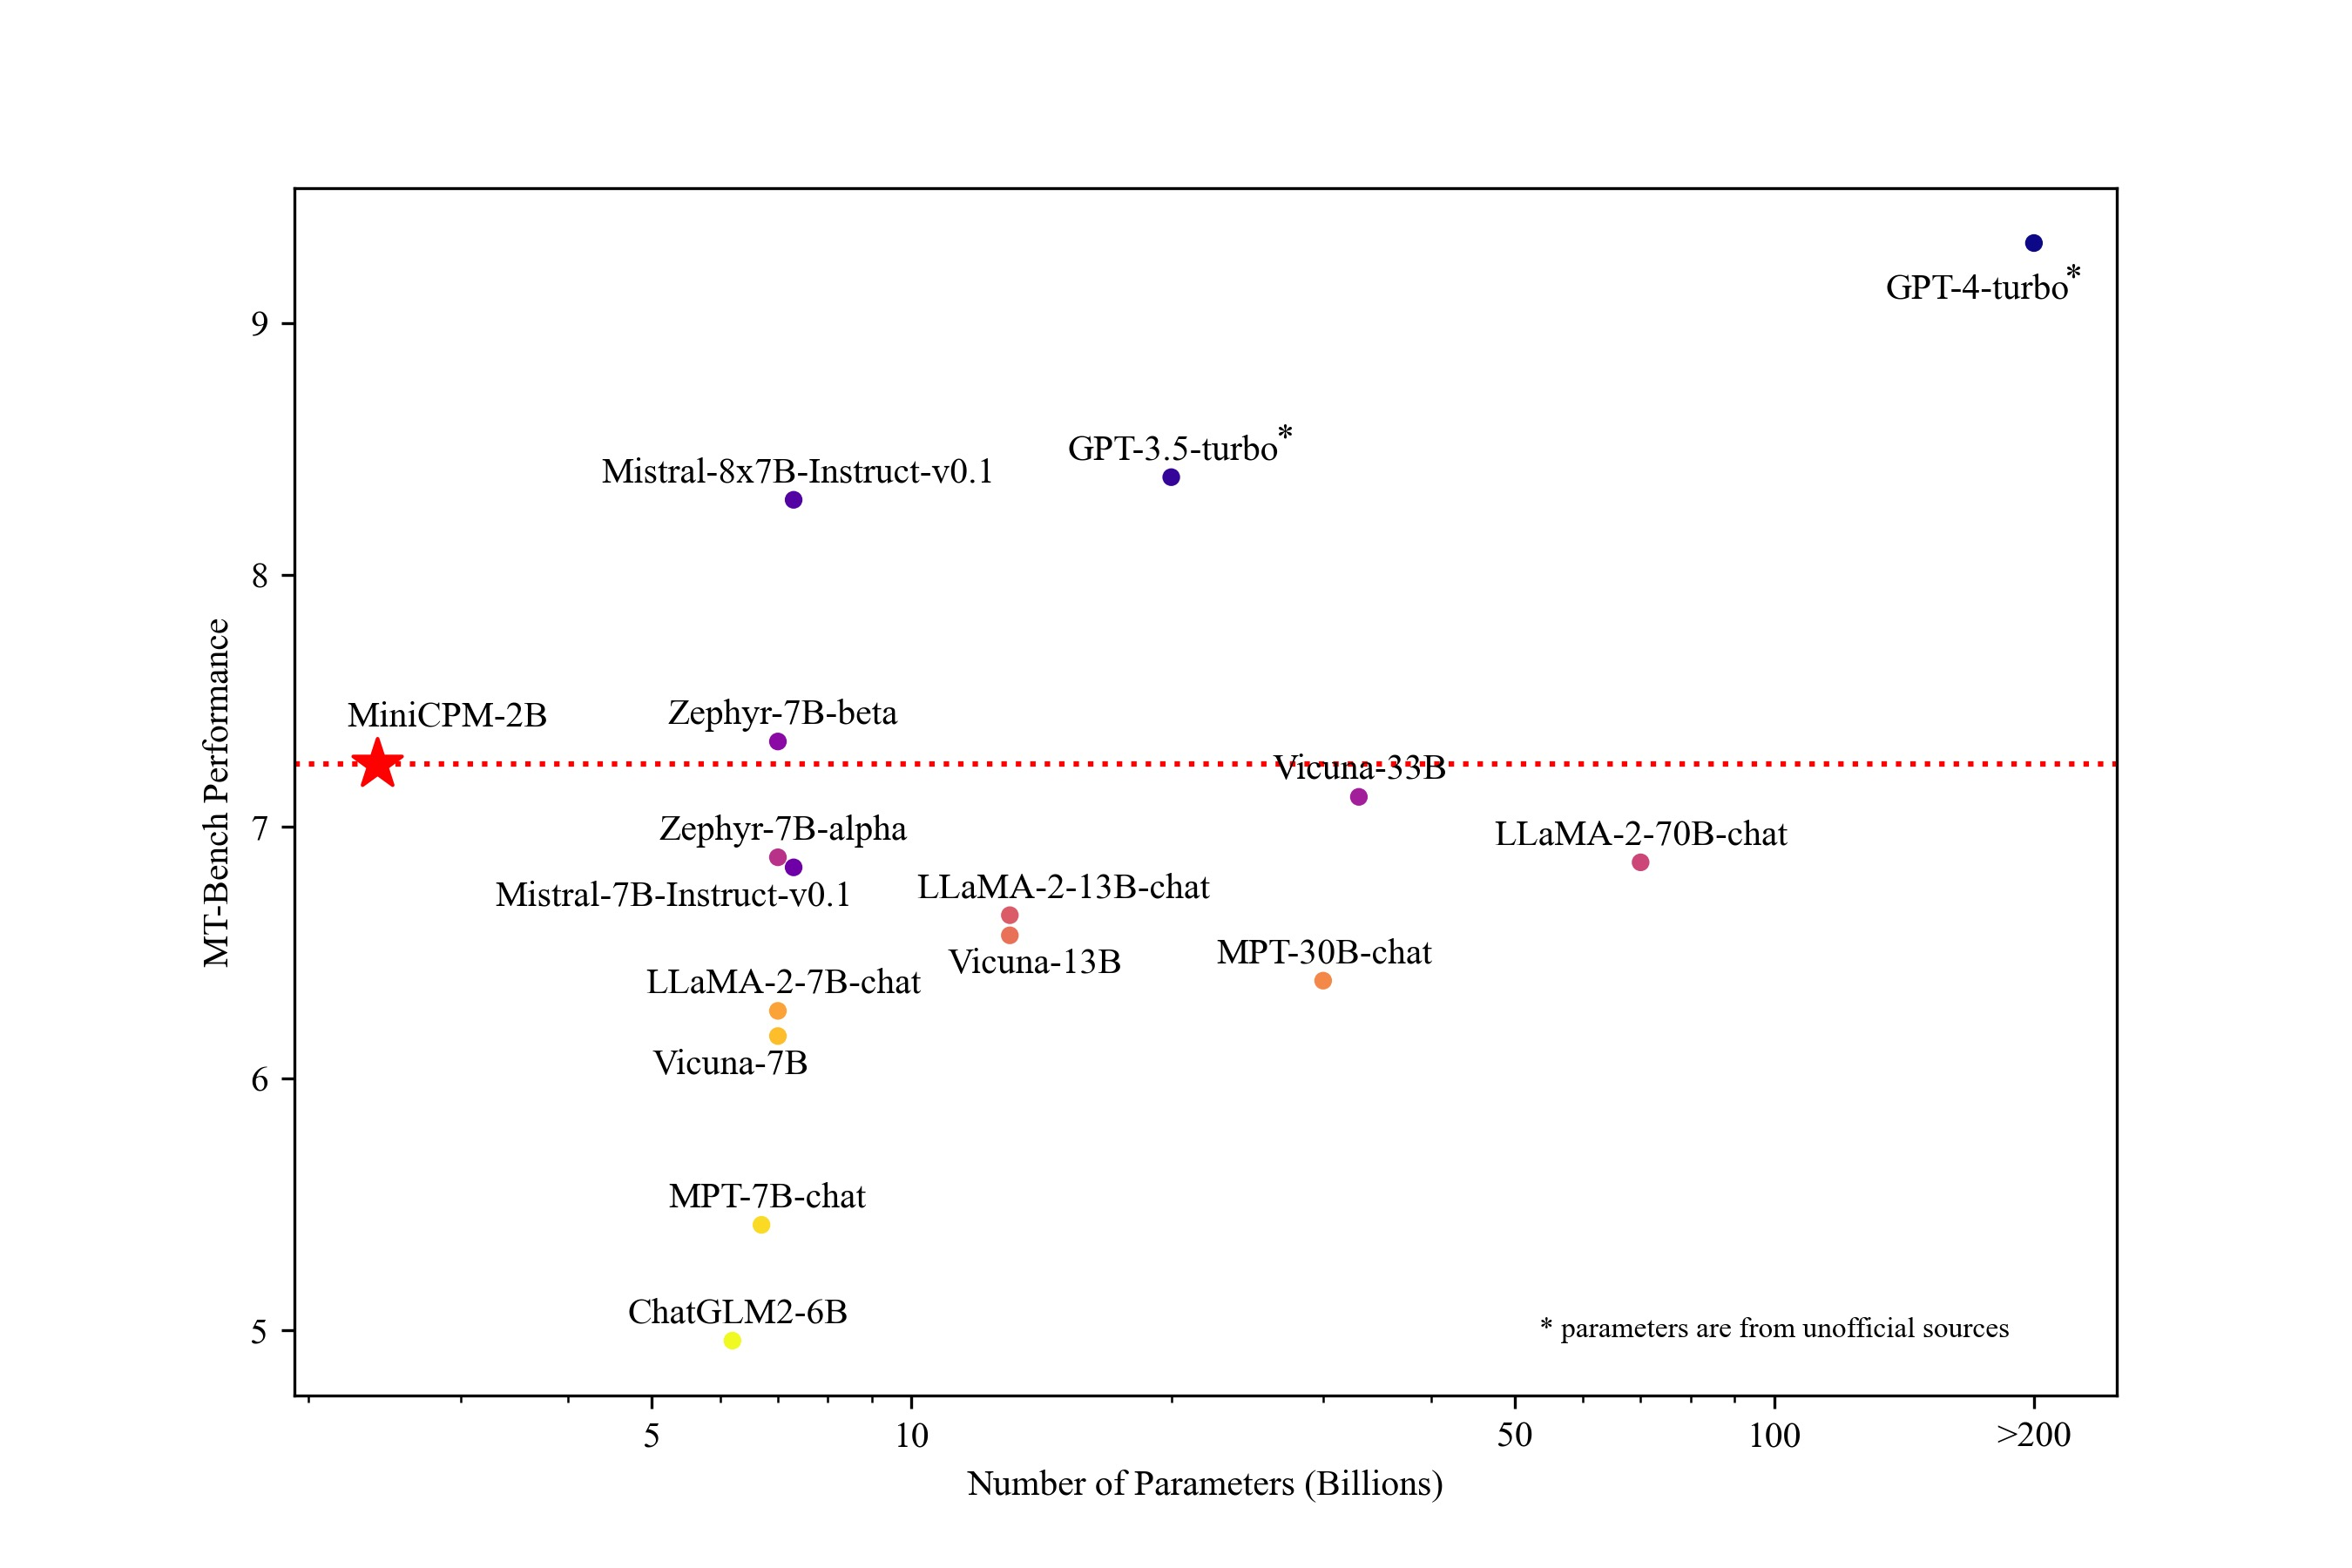
\includegraphics[width=\linewidth]{minicpmFig/mtbench_graph.jpg}
    \caption{MiniCPM - DPO - 2.4B的MTBench得分超过了许多更大规模的模型。}
    \label{fig:mtbenchscore}
\end{figure}

\section{模型能力展示}
MiniCPM系列与微软的Phi~\citep{li2023textbooks}等其他强大的小语言模型(SLMs)相比,一个显著区别在于,我们使用通用语料库来训练MiniCPM,这确保了模型在各种任务中的通用性和泛化能力。在本节中,我们展示几个通常只有更大规模模型才能实现的有趣生成实例,以展现MiniCPM的能力。尽管我们并未对训练集中是否存在特定案例进行广泛排查,但考虑到这些案例的表达方式多样,我们确保没有刻意添加与测试案例相似的数据。 

\begin{figure}[!h]
    \centering
    \scalebox{0.95}{
    \begin{AIbox}{Translation}
    {\bf Prompt:} 
    {\scriptsize
    Translate this sentence into French: "I am a freshman on Chinese, do you know how this sentence is translated: {如何用Python创建一个简单的网页爬虫?" (\textcolor{darkgreen}{How to create a simple web crawler in Python?})
    }}\\\ \\
    \parbox[t]{0.49\linewidth}{{\bf MiniCPM-1.2B:}\\
    \scriptsize
    Je suis un homme nouveau en chinois, vous êtes-vous au courant de la manière dont cette phrase est traduite : Comment créer un petit scraper web simple à Python ?
    }\hspace{0.02\linewidth}%
    \parbox[t]{0.49\linewidth}{{\bf MiniCPM-2.4B-DPO:} \\
    \scriptsize
    Je suis un nouveau-né en chinois, sais-tu comment on crée un simple web crawler en Python ?
    Translation: "Je suis un nouveau-né en chinois, sais-tu comment on crée un simple web crawler en Python ?"
    }
    \hspace{0.01\linewidth}
    \end{AIbox}
    }
    \caption{Examples on translation. We notice that MiniCPM-2.4B-DPO performs better in translating the technical part, but both models are unnatural in expressing "just starting to learn Chinese.". However, both models successfully understand the instruction with traps and generate French despite we do not include French corpus intentionally.}
    \label{fig:translation_example}
\end{figure}
    
    
\begin{figure}[!h]
    \centering
    \scalebox{0.95}{
    \begin{AIbox}{Math and Reasoning}
    {\bf Prompt:} 
    {\scriptsize
    {如果以下算式中减号均表示加号,而加号实际上是减号,给出算式的计算结果15-25-12+34=
    }\\ (\textcolor{darkgreen}{If in the following equation, minus signs represent addition, and plus signs represent subtraction, give the result of the calculation: 15-25-12+34=})}\\\ \\
    \parbox[t]{0.49\linewidth}{{\bf MiniCPM-1.2B:}\\
    \scriptsize
    {如果减号表示加号,那么我们可以将算式改写为:15 + 25 + 12 - 34 \\ \\
    首先计算前两个数的和:15 + 25 = 40\\
    然后计算前三个数的和:40 + 12 = 52\\
    最后计算最后一个数减去前三个数的和:52 - 34 = 18\\ \\
    所以,算式的计算结果为18。}\\(\textcolor{darkgreen}{If the minus sign represents a plus sign, then we can rewrite the equation as: 15 + 25 + 12 - 34.\\ \\
    First, calculate the sum of the first two numbers: 15 + 25 = 40. \\
    Then, calculate the sum of the first three numbers: 40 + 12 = 52. \\
    Finally, calculate the difference between the last number and the sum of the first three numbers: 52 - 34 = 18. \\ \\
    Therefore, the result of the equation is 18.})
    }
    \hspace{0.02\linewidth}%
    \parbox[t]{0.49\linewidth}{{\bf MiniCPM-2.4B-DPO:} \\
    \scriptsize
    {如果减号均表示加号,而加号实际上是减号,那么算式可以重新表示为:\\
    15+25+12-34\\ \\
    现在我们可以按照加减法的顺序进行计算:\\
    (15+25)+12-34=40+12-34=52-34=18\\ \\
    所以,最终的计算结果是 18。}\\(\textcolor{darkgreen}{If minus signs all represent addition, and plus signs actually represent subtraction, then the equation can be re-expressed as:\\
    15+25+12-34.\\ \\
    Now we can calculate according to the order of addition and subtraction:\\
    (15+25)+12-34 = 40+12-34 = 52-34 = 18\\ \\
    So, the final result of the calculation is 18.})
    }
    \hspace{0.01\linewidth}
    \end{AIbox}
    }
    \caption{Examples on math and reasoning. Both models are successful in symbolic substitution and math calculation.}
    \label{fig:math}
    \end{figure}
    
    \begin{figure}[!b]
    \centering
    \scalebox{0.95}{
    \begin{AIbox}{Instruction Following}
    {\bf Prompt:} 
    {\scriptsize
    {写藏头诗,藏头是龙年大吉
    }\\ (\textcolor{darkgreen}{Writing an acrostic poem, with the hidden message "Good luck in the Year of the Dragon."})}\\\ \\
    \parbox[t]{0.49\linewidth}{{\bf MiniCPM-1.2B:}\\
    \scriptsize
    {龙池春水涨,\\凤阙日初长。\\吉庆何时至,\\太平有象藏。}\\(\textcolor{darkgreen}{The spring water in the dragon's pool rises,\\
    The sun rises at the phoenix gate.\\
    When will good fortune arrive,\\
    Peace and prosperity are hidden in signs.})
    }
    \hspace{0.02\linewidth}%
    \parbox[t]{0.49\linewidth}{{\bf MiniCPM-2.4B-DPO:} \\
    \scriptsize
    {龙腾万里气如虹,\\
    年岁新来乐事浓。\\
    大吉良辰堪共赏,\\
    吉祥如意笑颜红。} \\(\textcolor{darkgreen}{Dragons soar for thousands of miles, their energy like a rainbow,\\
    As the new year begins, joyous occasions abound.\\
    Auspicious days are worth enjoying together,\\
    Good fortune and happiness bring rosy smiles.})
    }
    \hspace{0.01\linewidth}
    \end{AIbox}
    }
    \caption{Examples on instruction following. MiniCPM-2.4B-DPO successfully follows the instructions and generates a poem with the correct tonal pattern and the first character of each sentence. However, MiniCPM-1.2B only generates the correct tonal pattern.}
    \label{fig:instruction}
    \end{figure}
    
    
    
    \begin{figure}[]
    \centering
    \scalebox{0.95}{
    \begin{AIbox}{Emoji}
    {\bf Prompt:} 
    {\scriptsize
    {请给我一个json,每个key是一个emoji, 每个value是这个emoji对应的意思,给出10个左右
    }\\ (\textcolor{darkgreen}{Please give me a JSON object where each key is an emoji and each value is the meaning of that emoji, providing around 10 examples.})}\\\ \\
    \parbox[t]{0.49\linewidth}{{\bf MiniCPM-1.2B:}\\
    \scriptsize
    {当然可以,这是一个包含10个左右emoji及其含义的JSON:\\
    \{\\
    "
\includegraphics[height=10pt]{minicpmFig/smiling-face-with-smiling-eyes_1f60a.png}": "笑容", \\
    "
\includegraphics[height=10pt]{minicpmFig/face-with-tears-of-joy_1f602.png}": "笑", \\
    "
\includegraphics[height=10pt]{minicpmFig/smiling-face-with-heart-eyes_1f60d.png}": "惊叹", \\
    "
\includegraphics[height=10pt]{minicpmFig/face-blowing-a-kiss_1f618.png}": "亲吻", \\
    "
\includegraphics[height=10pt]{minicpmFig/winking-face-with-tongue_1f61c.png}": "恶作剧",\\
    "
\includegraphics[height=10pt]{minicpmFig/pensive-face_1f614.png}": "失望", \\
    "
\includegraphics[height=10pt]{minicpmFig/thinking-face_1f914.png}":"思考", \\
    "
\includegraphics[height=10pt]{minicpmFig/money-mouth-face_1f911.png}": "金钱",\\
    "
\includegraphics[height=10pt]{minicpmFig/folded-hands_1f64f.png}": "帮助",\\
    "
\includegraphics[height=10pt]{minicpmFig/pile-of-poo_1f4a9.png}": "废物"\\
    \} \\
    希望这个JSON对你有帮助!} \\ (\textcolor{darkgreen}{Of course, this is a JSON file containing around 10 emojis and their meanings:\\
    \{\\
    "
\includegraphics[height=10pt]{minicpmFig/smiling-face-with-smiling-eyes_1f60a.png}": "smiling", \\
    "
\includegraphics[height=10pt]{minicpmFig/face-with-tears-of-joy_1f602.png}": "laughing", \\
    "
\includegraphics[height=10pt]{minicpmFig/smiling-face-with-heart-eyes_1f60d.png}": "amazing", \\
    "
\includegraphics[height=10pt]{minicpmFig/face-blowing-a-kiss_1f618.png}": "kissing", \\
    "
\includegraphics[height=10pt]{minicpmFig/winking-face-with-tongue_1f61c.png}": "mischief",\\
    "\includegraphics[height=10pt]{minicpmFig/pensive-face_1f614.png}": "disappointment", \\
    "\includegraphics[height=10pt]{minicpmFig/thinking-face_1f914.png}":"thinking", \\
    "\includegraphics[height=10pt]{minicpmFig/money-mouth-face_1f911.png}": "money",\\
    "\includegraphics[height=10pt]{minicpmFig/folded-hands_1f64f.png}": "help",\\
    "\includegraphics[height=10pt]{minicpmFig/pile-of-poo_1f4a9.png}": "rubbish"\\
    \} \\
    Hope you found this JSON useful!})
    }
    \hspace{0.02\linewidth}%
    \parbox[t]{0.49\linewidth}{{\bf MiniCPM-2.4B-DPO:} \\
    \scriptsize
    {当然可以!以下是一个包含10个emoi及其对应意义的JSON对象:\\
    \{\\
    "\includegraphics[height=10pt]{minicpmFig/smiling-face-with-smiling-eyes_1f60a.png}": "表示愉快或满意,通常用于表达微笑和喜悦。", \\
    "\includegraphics[height=10pt]{minicpmFig/pouting-face_1f621.png}": "表示愤怒或不满,通常用于表达情绪的激动。", \\
    "\includegraphics[height=10pt]{minicpmFig/face-with-tears-of-joy_1f602.png}": "表示大笑或开心,通常用于表达笑声和欢乐。", \\
    "\includegraphics[height=10pt]{minicpmFig/rolling-on-the-floor-laughing_1f923.png}": "表示搞笑或尴尬,通常用于表达搞笑的场景或尴尬的情况。", \\
    "\includegraphics[height=10pt]{minicpmFig/exploding-head_1f92f.png}": "表示惊讶或震惊,通常用于表达对某个事件或情況的强烈反应。",\\
    "\includegraphics[height=10pt]{minicpmFig/pensive-face_1f614.png}": "表示失望或沮丧,通常用于表达对某事或某人失去兴趣或信心的情绪。", \\
    "\includegraphics[height=10pt]{minicpmFig/broken-heart_1f494.png}":"表示心痛或伤心,通常用于表达对某事或某人造成痛苦的强烈感受。", \\
    "\includegraphics[height=10pt]{minicpmFig/light-bulb_1f4a1.png}": "表示惊喜或兴奋,通常用于表达对某事或某人的发现或发现的情绪。",\\
    "\includegraphics[height=10pt]{minicpmFig/smiling-face-with-smiling-eyes_1f60a.png}": "表示酷或时髦,通常用于表达自信、独立和潮流的态度。",\\
    "\includegraphics[height=10pt]{minicpmFig/smiling-face-with-heart-eyes_1f60d.png}": "表示喜欢或欣赏,通常用于表达对某物或某人的喜爱之情。"\\
    \} \\
    希望这个JSON对象能满足您的需求!如果您有任何问题,请随时告诉我。} \\(\textcolor{darkgreen}{Of course! Here is a JSON object containing 10 emojis and their corresponding meanings:\\
    \{\\
    "\includegraphics[height=10pt]{minicpmFig/smiling-face-with-smiling-eyes_1f60a.png}": "It means happy or satisfied, typically used to express smiling and joy.", \\
    "\includegraphics[height=10pt]{minicpmFig/pouting-face_1f621.png}": "It means anger or dissatisfaction, typically used to express intense emotions.", \\
    "\includegraphics[height=10pt]{minicpmFig/face-with-tears-of-joy_1f602.png}": "It means laughing or happy, typically used to express laughter and joy.", \\
    "\includegraphics[height=10pt]{minicpmFig/rolling-on-the-floor-laughing_1f923.png}": "It means funny or awkward, typically used to express humorous situations or awkwardness.", \\
    "\includegraphics[height=10pt]{minicpmFig/exploding-head_1f92f.png}": "It means surprise or shock, typically used to express a strong reaction to an event or situation.",\\
    "\includegraphics[height=10pt]{minicpmFig/pensive-face_1f614.png}": "It means disappointment or discouragement, typically used to express a loss of interest or confidence in something or someone.", \\
    "\includegraphics[height=10pt]{minicpmFig/broken-heart_1f494.png}": "It means heartache or sadness, typically used to express intense feelings of pain caused by something or someone.", \\
    "\includegraphics[height=10pt]{minicpmFig/light-bulb_1f4a1.png}": "It means surprise or excitement, typically used to express the emotion of discovery or finding something or someone.",\\
    "\includegraphics[height=10pt]{minicpmFig/smiling-face-with-smiling-eyes_1f60a.png}": "It means cool or stylish, typically used to express a confident, independent, and trendy attitude.",\\
    "\includegraphics[height=10pt]{minicpmFig/smiling-face-with-heart-eyes_1f60d.png}": "It means like or appreciate, typically used to express affection or admiration for something or someone."\\
    \} \\
    I hope this JSON object meets your needs! If you have any questions, please feel free to let me know.})
    }
    \hspace{0.01\linewidth}
    \end{AIbox}
    }
    \caption{Examples on emoji. Both models understand emojis and structured data well, and accurately control the number of items implicitly. The DPO model tends to generate more words. }
    \label{fig:emoji}
    \end{figure}
\chapter{总结与展望}

\section{研究工作总结}

语言模型是自然语言处理乃至人工智能的核心研究领域之一,近年来,大语言模型的研究与应用取得了长足进展。大语言模型通过大规模预训练和高质量数据微调获得了极高的通用性和专业性,成为当前迈向通用人工智能的最有潜力的路线。大语言模型的智能提升遵循扩展定律,这表明其性能随训练资源增加而提高。然而,由于人类资源的有限性,这已成为制约大语言模型智能发展的核心瓶颈之一。

当前大语言模型训练已进入百万亿参数时代,其资源消耗呈指数级增长趋势。以OpenAI的GPT-4为例,其训练需要消耗约$10^25$次浮点计算,资金开销在数亿美元级别。扩展定律揭示的性能与模型规模、数据量、计算量的幂律关系,使追求更大规模模型成为必然选择。然而,人类短期内资源总量有限,如何提高资源利用效率已成为当前人工智能领域亟待解决的重要问题。

本文致力于减少大语言模型训练过程中的资源消耗,从而促进模型规模的进一步发展。具体而言,本文研究了大语言模型训练过程中两个主要阶段——预训练阶段和微调阶段——各自面临的资源挑战。对于预训练阶段,不可预测性导致预训练反复调优,进而浪费了大量资源;对于微调阶段,高质量数据消耗量大和微调参数冗余度高导致了微调的资源浪费。因此,本文提出了可预测预训练和低资源微调两个研究目标,并取得了一系列重要进展。

本文的主要研究内容与贡献如下:

\begin{enumerate}

\item \textit{面向可预测预训练的超参数扩展规律与性能扩展定律。} 

本研究首先基于Tensor Program进行探索,在真实场景对tensor program进行了深入研究,发现在辅以批量大小的扩展方案时,可以获得稳定的学习率扩展规律。本研究还对其他结构变体,例如QK-Norm,是否能对超参数稳定起到关键作用进行了研究。 在得到稳定的超参扩展规律带来的损失扩展规律后,本研究深入探索了性能扩展规律。性能扩展定律被认为是非常困难的,因为任务性能不仅影响因素众多,还会表现出波动性和涌现性(即涌现能力)。针对这个问题,本研究进行了深入实验,提出了一种基于大量采样的提升模型评估分辨率的方法,证明了这一方法是真实表现的无偏估计,并且假如计算资源允许,可以精确到任意精度。本研究进一步提出了性能扩展定律,区别于损失扩展定律,该定律可以直接对下游任务性能进行预测。引入了数据集级别扩展和样本级别扩展两种方案,并提出损失辅助预测方法。这些方法将性能预测精度提升到99\%以上,初步解决了性能扩展规律的问题,避免了大规模预训练实验的反复试错,大幅降低了训练资源消耗。

\item \textit{面向可预测预训练的可复用扩展定律与高效退火迭代。} 

本研究分析了进行扩展定律拟合过程中的资源消耗,发现现有文献的拟合方法需要消耗的计算量和调研模型参数规模个数以及调研数据规模个数都成线性关系,因此在数据和模型两个维度的扩展定律研究需要消耗平方复杂度的算力。本研究思考了不同数据量下的模型训练无法复用训练过程的原因,将其归结为学习率调度对损失的影响带来的不可复用性。 本研究分析了当前绝大部分模型训练都使用的学习率调度策略,提炼出其效果优异的原因,即同时具备全局最优解寻找和局部最优解寻找(退火)的特点。本研究提出将占训练过程绝大部分时间的全局最优解进行多模型共享,再通过时机各异的局部最优解寻找来完成模型训练。研究证明,这种方法使数据维度的扩展定律拟合消耗的资源变为常数量级,有效提高了扩展定律拟合过程的高效性。本研究进一步实验指出,基于以上策略的扩展定律拟合方法,由于其可复用的退火阶段,使得高质量数据迭代实验变得非常高效。研究仔细分析了退火过程中引入不同数据对于模型训练结果的影响,发现在退火过程中引入高质量数据能显著提高模型在下游任务上的表现。由于可复用的退火阶段在整个训练过程占比很小,所以可以使用少量的算力进行多次性能迭代。此外,本研究还探索了退火迭代的训练动力学方面的原因,为后人对训练机理的探索提供了新的方向。综合利用上述方法,本研究利用1/7的算力和1/3的模型大小,训练了性能超越Llama2-7B的模型,充分证明了本研究方案的有效性和实用价值。

\item \textit{面向低资源微调的能力激发与知识激活。} 

本研究从微调阶段的数据角度出发,首先研究了预训练模型对于分布外任务是否可以使用少量数据习得。以"错误先验立场"问题为例开展研究,该类问题的特点是回答所需知识存在于大语言模型的预训练阶段,但由于分布差异导致模型无法有效调用这些知识进行回答。本研究首次提供了精标注的人类对于"错误先验立场"问题的回答,证明只需要百到千量级的数据,就可以将模型的回复正确率从随机水平提升到接近90\%的准确率。这一发现提供了"小数据激活大能力"的有力证据,该思路也在后续的Instruction Tuning以及RLHF等工作中得到了进一步验证。本研究进一步探索了对于与预训练模型能力更为接近的分布内任务,例如情感分类和主题分类,是否可以通过更少量的样本或者零样本来进行适配。知识微调是大模型范式下的有效适配手段,其利用模板和表达器来完成模型训练分布到任务输入输出空间的变换。本研究提出了知识提示微调的概念,即在提示微调的基础上,引入知识库扩充的表达器,使得模型在微调过程中可以更好地利用预训练模型的知识。研究表明,通过在提示微调的表达器中引入人类知识先验,能够将模型性能提升高达17\%,大幅降低了所需样本量。

\item \textit{面向低资源微调的参数高效微调模块自动化寻优。} 

本研究从微调阶段的存算资源角度出发,研究了参数高效微调的自动化模块选择功能。传统参数高效微调的方法会选择默认模块进行微调。尽管这种方法能够大幅减少需要微调的参数量,然而由于在预训练过程中,不同模块已经训练出不同的分工,微调时使用默认模块可能会导致模型性能不能充分发挥。本研究提出了一种基于自动化模块选择的参数高效微调框架,该框架建立在对所有参数高效微调方法的统一建模视角下,借鉴了神经架构自动搜索算法,并创新地提出了可训练硬稀疏化优化目标,精准控制可微调参数总量。本研究使参数高效微调所需的微调参数量从全参数的1\%进一步降低到0.01\%量级,大幅减少了存算资源需求。
% 本研究同时提供了一个灵活轻便的参数高效微调代码库,在实现上通过"猴子补丁"的方式灵活修改预训练模型的张量流,使其能够动态加载和移除任意位置的参数高效微调模块,也可以同时加载多个参数高效微调模块,甚至组合不同种类的参数高效微调模块。在用户体验上,本代码库提供了一套完整的参数高效微调模块接口,用户可以通过简单的配置文件,即可实现对预训练模型的参数高效微调,极大地降低了技术门槛。

\end{enumerate}

总结来说,本文对大语言模型训练全流程提出了高效解决方法,这些方法有利于模型进一步进行规模扩展以实现更高的智能上限。本文的主要贡献可以概括为四个方面:(1)提出了超参数扩展规律与性能扩展定律,实现了对下游任务性能的高精度预测;(2)提出了可复用扩展定律与高效退火迭代技术,显著降低了扩展定律拟合的资源消耗;(3)研究了能力激发与知识提示微调方法,以极少样本实现模型能力的有效激活;(4)提出了参数高效微调模块自动化寻优框架,将微调参数量降至全参数的万分之一量级。

与此同时,本文的研究成果对包括模型训练机理、模型参数功能分区、模型涌现能力成因等方面都提供了新的见解。这些创新不仅降低了大模型训练的资源门槛,也为推动人工智能领域的可持续发展做出了重要贡献。

\section{未来工作展望}

大语言模型高效训练研究仍处于高速发展阶段,并且训练方法本身也在同步演进,例如RLHF训练、多模态统一训练。未来可以从以下几个方向继续深入探索:

\begin{enumerate}

\item \textit{大规模强化学习扩展规律和超参数定律。} 

继大规模预训练以后,大规模强化学习将成为下一个主要资源消耗阶段。尽管当前RLHF应用虽已广泛,但其背后的扩展规律仍处于经验探索阶段,缺乏系统性理解。并且以O1、R1为代表的长思维链强化学习技术,尚处于萌芽阶段。未来研究将揭示强化学习中参数规模、训练轮次、奖励信号复杂度与涌现能力间的定量关系,建立类似于监督学习中已有的扩展定律。理解这些规律将使我们能够预测训练资源投入与回报之间的关系,从而做出更合理的资源分配决策。从长远来看,强化学习扩展规律研究将推动理解人类反馈与模型能力提升间的复杂关系,揭示人类价值观如何在大模型中被有效表达和强化。这不仅具有理论价值,也将为解决AI对齐问题提供实证基础,可能成为安全可控AI发展的重要理论支柱。

\item \textit{多模态统一训练扩展规律。} 

多模态统一训练扩展规律研究将致力于揭示跨越视觉、语言、音频等不同感知通道的统一学习机制,同时必须深入探索模态间干扰现象这一核心挑战。当前多模态研究已经观察到"负迁移"现象——模型在整合多模态信息过程中,一种模态的引入有时会损害其他模态的表征质量,使得联合训练性能反而低于单模态训练。这种模态冲突现象尚未纳入现有扩展理论框架,理解其机制将成为未来研究的关键突破点。

\item \textit{硬件感知的预训练优化。} 

未来硬件感知的预训练优化研究将突破当前算法与硬件分离设计的局限,向着全栈协同优化的方向发展。随着专用AI芯片架构日益多元化,预训练算法将不再以通用计算为目标,而是根据底层硬件特性进行根本性重构。这种范式转变意味着算法设计者需要深入理解硬件架构特性,而硬件设计者也需要考虑大模型训练的算法需求,形成一种双向反馈的协同设计思路。相应的,扩展定律也应该考虑到不同超参数在性能和计算效率上的双面影响,综合考虑和设计预训练扩展方案。

\item \textit{大模型训练机理。} 


大模型训练机理研究将从实践中的经验积累转向系统的理论构建,致力于回答“为什么大模型能够有效”、“大模型训练发生了什么”这些根本问题。当前,大模型的许多能力尤其是涌现能力,往往是意外发现而非设计所得,这反映出我们对深度学习本质的理解仍然有限。未来研究将不满足于对现象的描述,而是追求揭示背后的原理。本文所提出的WSD调度揭示,我们对大模型的优化理论理解尚浅,目前尚不存在理论可以定量解释大模型退火阶段下降的损失幅度。在这一方向进一步研究将促进深度学习与其他科学领域如统计学、信息几何学等深度融合,可能形成全新的理论框架。通过对大模型内部表征形成、推理路径的深入分析,研究者将能够构建起描述神经网络规模、优化方案与最终性能之间关系的数学模型,为未来模型设计提供理论指导。

\end{enumerate}
\chapter{少资源微调——基于知识融合的少样本微调}

使用特定任务提示对预训练语言模型进行微调,已成为文本分类中一种很有前景的方法。特别地,以往研究表明,在数据量少的场景下,提示微调相较于使用额外分类器的通用微调方法具有显著优势。提示微调的核心思想是在输入中插入文本片段,即模板,并将分类问题转化为掩码语言建模问题,其中关键一步是在标签空间和标签词空间之间构建一个投影,即语言表达器(verbalizer)。语言表达器通常是手工制作的,或者通过梯度下降搜索得到,这可能会导致覆盖范围不足,并给结果带来相当大的偏差和高方差。在这项工作中,我们专注于将外部知识融入语言表达器,形成一种\textbf{知识型提示微调}(KPT),以改进并稳定提示微调。 

\section{方法设计}

\subsection{提示微调概述}
设 ${\mathcal{M}}$ 为在大规模语料库上预训练的语言模型。

在文本分类任务中,输入序列 $\mathbf{x} = (x_0,x_1,...,x_n)$ 被分类为类别标签 $y\in \mathcal{Y}$。提示微调将分类任务形式化为掩码语言建模问题。具体来说,提示微调将输入序列包裹在一个\emph{模板}中,模板是一段自然语言文本。

例如,假设需要将句子 $\mathbf{x}$ =“速度与加速度之间的关系是什么?”分类为标签 \textsc{科学}(标记为1)或 \textsc{体育}(标记为2),本文将其包裹为

\begin{equation*}
    \mathbf{x}_{\text{p}}=\text{\texttt{[CLS]} 一个 \texttt{[MASK]} 问题:} \mathbf{x}
\end{equation*}
然后 ${\mathcal{M}}$ 给出词汇表中每个词 $v$ 填入 \texttt{[MASK]} 标记的概率 $P_{\mathcal{M}}(\texttt{[MASK]}=v|\mathbf{x}_{\text{p}})$。
为了将词汇的概率映射到标签的概率,本文定义了一个\emph{语言表达器},即从词汇表中的少量词(构成\emph{标签词}集 $\mathcal{V}$)到标签空间 $\mathcal{Y}$ 的映射 $f$,即 $f\colon \mathcal{V} \mapsto \mathcal{Y}$。本文用 $\mathcal{V}_y$ 表示映射到特定标签 $y$ 的 $\mathcal{V}$ 子集,$\cup_{y\in\mathcal{Y}} \mathcal{V}_y = \mathcal{V}$。然后标签 $y$ 的概率 $P(y|\mathbf{x}_{\text{p}})$ 计算为


\begin{equation}
   P(y|\mathbf{x}_{\text{p}}) \!\!=\!\! g\left(P_{\mathcal{M}}(\texttt{[MASK]}\!\!\!=\!v|\mathbf{x}_{\text{p}})|v\in\mathcal{V}_y\right),
\end{equation}


其中$g$是将标签词的概率转换为标签概率的函数。
在上述例子中,常规提示微调可能定义 $\mathcal{V}_1=\{\text{``科学''}\}$,$\mathcal{V}_2=\text{\{``体育''}\}$,并将 $g$ 定义为恒等函数,那么如果“科学”的概率大于“体育”,则将句子分类为 \textsc{科学}。

本文提出了KPT,主要关注利用外部知识改进提示微调中的语言表达器。
在KPT中,本文使用知识库为每个类别 $y$ 生成多个相关标签词,例如 $\mathcal{V}_1 = \text{\{``科学'',``物理'', ...\}}$。并提出了四种优化方法来消除扩展后的 $\mathcal{V}$ 中的噪声。最后,本文探索了扩展 $\mathcal{V}$ 的简单平均和加权平均方法。
细节将在以下部分中介绍。

\begin{figure*}[!htbp]
  \centering
\scalebox{0.97}{
  \includegraphics[width = \linewidth]{kptplots/framework.pdf}
  }
  \caption{KPT框架示意图。KPT将对标签词的预测映射为标签。上述部分是KPT的构建、细化以及利用过程。}
  \label{fig:my_label}
\end{figure*}


\subsection{语言表达器构建}
\label{sec:cons}

基于上下文预测掩码词的过程不是单一选择过程,即没有标准正确答案,而是有许多词可能适合该上下文。
因此,语言表达器映射的标签词应具备两个属性:\textit{广泛覆盖}和\textit{较少主观偏差}。这种全面的映射对于模仿预训练至关重要,而预训练是提示微调能力的来源。外部结构化知识可以同时满足这两个要求。在本节中,本文介绍了如何利用外部知识进行两种文本分类任务:主题分类和情感分类。

对于主题分类,核心问题是从所有方面和粒度中提取与主题相关的标签词。从这个角度出发,本文选择了Related Words~\footnote{\url{https://relatedwords.org}},这是一个从多个资源(包括词嵌入、ConceptNet~\cite{speer2017conceptnet}、WordNet~\cite{pedersen2004wordnet}等)聚合的知识图谱 $\mathcal{G}$ 作为外部知识库。
边表示“相关性”关系,并标注了相关性分数。本文假设每个类别的名称 $v_0$ 是正确的,并将其作为锚点获取邻域节点 $N_{\mathcal{G}}(v_0)$,其分数大于阈值 $\eta$ 作为相关词~\footnote{实验中取 $\eta=0$}。因此,每个类别被映射到一组标签词 $\mathcal{V}_{y} = N_{\mathcal{G}}(v_0) \cup \{v_0\}$。
对于二元情感分类,主要目标是扩展二元情感到更多粒度和方面的情感。本文使用了之前研究人员总结的情感词典~\footnote{\url{https://www.enchantedlearning.com/wordlist/positivewords.shtml}}$^{,}$\footnote{ \url{https://www.enchantedlearning.com/wordlist/negativewords.shtml}}。
KPT中标签词的几个示例如表~\ref{tab:label_words_examples}所示。

\begin{table*}[!htbp]
    \centering
    \caption{扩展标签词的示例。}
\scalebox{0.93}{
    \begin{tabular}{ccl}
    \toprule
  数据集 &  标签 & \multicolumn{1}{c}{标签词} \\
    \midrule
  \multirow{2}{*}{AG's News}  &  \textsc{政治} &  政治, 政府, 外交, 法律, 亚里士多德, 外交的, 治理 ...\\
    &  \textsc{体育}   & 体育, 运动, 体操, 运动员, 竞赛, 自行车, 足球 ... \\
      \midrule
 \multirow{2}{*}{IMDB} &    \textsc{负面} & 糟糕的, 不利的, 令人担忧的, 生气的, 烦恼的, 焦虑的, 冷漠的, 可怕的 ...\\
    &  \textsc{正面} & 绝对的, 接受的, 备受赞誉的, 完成, 成就  ...\\
      \bottomrule
    \end{tabular}
}
    \label{tab:label_words_examples}
\end{table*}

\subsection{语言表达器优化}
\label{sec:refine}

尽管构建了一个包含全面标签词的知识化语言表达器,但由于知识库的词汇并非为预训练语言模型量身定制,收集的标签词可能非常嘈杂。因此,有必要通过保留高质量词来优化语言表达器。在本节中,本文提出了四种优化方法,分别解决嘈杂标签词的不同问题。

\textbf{频率优化。} 第一个问题是处理罕见词。本文假设知识库中的某些词对预训练语言模型来说是罕见的,因此这些词的预测概率往往不准确。我提出使用标签词的\emph{上下文先验}来去除这些词。具体来说,给定一个文本分类任务,本文表示语料库中句子 $\mathbf{x}$ 的分布为 $\mathcal{D}$。对于分布中的每个句子,我将其包裹到模板中,并计算每个标签词 $v$ 在掩码位置的预测概率 $P_{\mathcal{M}}(\texttt{[MASK]}\!\!\!=\!v|\mathbf{x}_{\text{p}})$。通过对整个句子分布的概率取期望,可以得到标签词在掩码位置的先验分布。将其形式化为

\begin{equation}
 P_{\mathcal{D}}(v)\! =\! \mathbb{E}_{\mathbf{x}\sim \mathcal{D}} P_{\mathcal{M}}(\texttt{[MASK]}\!\!\!=\!v|\mathbf{x}_{\text{p}}).
\end{equation}
根据经验,本文发现使用从训练集中采样的小规模\emph{未标注支持集} $\tilde{\mathcal{C}}$ 并去除标签,可以很好地估计上述期望。因此,假设输入样本 $\{\mathbf{x}\in \tilde{\mathcal{C}}\}$ 具有均匀先验分布,上下文先验近似为
\begin{equation}
    P_{\mathcal{D}}(v) \approx \frac{1}{|\tilde{\mathcal{C}}|} \sum_{\mathbf{x}\in \tilde{\mathcal{C}}} P_{\mathcal{M}}(\texttt{[MASK]}\!\!\!=\!v|\mathbf{x}_{\text{p}}),
\end{equation}
然后移除先验概率小于阈值的标签词。由于上下文化先验概率的绝对值分布可能因任务而异,确定一个具体的上下文化先验概率阈值可能会非常难以捉摸。本文采用基于排序的阈值,即过滤掉出现在上下文化先验概率下半部分的标签词。

\textbf{相关性优化。}
由于本文构建的知识化标签词是完全无监督的,某些标签词可能比其他词更相关于其所属类别。
为了衡量标签词与每个类别的相关性,本文获取标签词在支持集 $\tilde{\mathcal{C}}$ 上的预测概率作为标签词的向量表示 $\mathbf{q}^{v}$,即 $\mathbf{q}^{v}$ 的第 $i$ 个元素为

\begin{equation}
    \mathbf{q}^{v}_i = P_{\mathcal{M}}([\texttt{MASK}]=v|\mathbf{x}_{i{\text{p}}}), \mathbf{x}_i\in \tilde{\mathcal{C}},
\end{equation}
其中 $\mathbf{x}_{i{\text{p}}}$ 表示句子 $x_i$ 与模板 $\text{p}$ 的组合。

为了估计类别的表示,本文假设每个类别的名称 $v_0$(例如“科学”对于 \textsc{科学})虽然覆盖范围有限,但与类别非常相关。然后本文使用这些名称的向量表示 $\mathbf{q}^{v_0}$ 作为类别的表示 $\mathbf{q}^{y}$。因此,标签词 $v$ 与类别 $y$ 之间的相关性得分计算为两个表示之间的余弦相似度:
\begin{equation}
    r(v, y) = \operatorname{cos}(\mathbf{q}^{v}, \mathbf{q}^{y}) = \operatorname{cos}(\mathbf{q}^{v}, \mathbf{q}^{v_0}).
\end{equation}

此外,某些标签词可能对多个类别有积极贡献,导致类别之间的混淆。例如,类别 \textsc{科学} 的潜在标签词“生理学”也可能在类别 \textsc{体育} 的句子中被赋予高概率。为了减轻这种混淆并过滤相关性较低的标签词,本文设计了一个指标,该指标偏好仅对其所属类别具有高相关性且对其他类别相关性较低的标签词:
\begin{equation}
    R(v) = r(v, f(v)) \frac{|\mathcal{Y}|-1}{\sum_{y\in \mathcal{Y}, y\neq f(v)}(r(v,y))},
\label{equ: rr_tfidf}
\end{equation}
其中 $f(v)$ 是 $v$ 对应的类别。

理想情况下,一个好的标签词至少应具有对其所属类别的高于其他类别平均相关性得分的相关性得分。因此,本文移除 $R(v)<1$ 的标签词。在实践中,本文对公式~\eqref{equ: rr_tfidf} 进行了轻微修改,这是因为本文观察到在只有少数类别的分类任务中,提供一个更严格的标准以确保标签词对\emph{任何其他}类别的相关性得分低于其对所属类别的得分是更好的选择,即优先选择IDF得分中的\emph{最大值}。为了保持统一的标准,本文使用基于范数的IDF得分:
\begin{equation}
    R^d(v)\! =\! r(v, f(v)) \large(\frac{|\mathcal{Y}|-1}{\sum_{y\in \mathcal{Y}, y\neq f(v)} r(v,y)^d}\large)^{1/d},
\end{equation}
其中
\begin{equation}
    d = \frac{C}{|\mathcal{Y}|-2+\epsilon} +1, C>0.
\end{equation}
该标准会使用标签个数对相关性分布进行锐化,在只有少数标签的分类任务中会近似于$\{r(v,y)|y\in |\mathcal{Y}|, y\neq f(v)\}$中的最大值,而在处理多标签分类时会退化为公式~\eqref{equ: rr_tfidf}中的平均得分。实验中取$C=10$(未经试错调整),且$0 < \epsilon\ll 1$是一个防止数值错误的小数。


本质上,这种相关性优化采用了经典TF-IDF~\cite{jones1972statistical}算法的思想,该算法估计词与文档的相关性。它偏好使用对特定文档相关而对其他文档不相关的词作为文档的关键词。在KPT中,类别类似于文档,而标签词类似于文档中的词。从这个角度来看,公式~\eqref{equ: rr_tfidf} 是TF-IDF度量的一种变体。 


\textbf{上下文校准。}\quad
\label{sec: refine-CC}
第三个问题是标签词先验概率的显著差异。正如之前的工作~\cite{pmlr-v139-zhao21c, holtzman2021surface}所示,某些标签词无论输入句子的标签如何,被预测的概率都较低,导致预测偏差。在本文的设置中,知识库中的标签词往往具有更多样化的先验概率,导致问题更加严重(见表~\ref{tab:experiment-zero-shot})。因此,本文使用标签词的上下文先验来校准预测分布,即上下文校准(Contextual Calibration, 简称CC):
\begin{equation}
    \tilde{P}_{\mathcal{M}}(\!\texttt{[MASK]}\!\!\!=\!v|\mathbf{x}_{\text{p}}) \!\propto\! \frac{P_{\mathcal{M}}(\!\texttt{[MASK]}\!\!\!=\!v|\mathbf{x}_{\text{p}})}{P_{\mathcal{D}}(v)},
\end{equation}
其中 $P_{\mathcal{D}}(v)$ 是标签词的先验概率。最终概率归一化为1。

\textbf{可学习优化}。在少样本学习中,优化可以通过学习过程加强。具体来说,本文为每个标签词 $v$(可能已经通过上述方法优化)分配一个可学习权重 $w_v$。权重形成一个向量 $\mathbf{w}\in \mathbb{R}^{|\mathcal{V}|}$,初始化为零向量。权重在每个 $\mathcal{V}_y$ 内归一化:

\begin{equation}
    \alpha_v = \frac{\operatorname{exp}(w_v)}{\sum_{u\in \mathcal{V}_y} \operatorname{exp}(w_u)}.
\end{equation}

直观上,在训练过程中,预计会为嘈杂的标签词学习到一个较小的权重,以最小化其对预测的影响。需要注意的是,在少样本设置中,校准可能不是必需的,因为标签词的概率可以被训练到所需的幅度,即 $\tilde{P}_{\mathcal{M}}(\texttt{[MASK]}\!\!\!=\!v|\mathbf{x}_{\text{p}}) ={P_{\mathcal{M}}(\texttt{[MASK]}\!\!\!=\!v|\mathbf{x}_{\text{p}})}$。

除了这些优化方法外,由于许多标签词对预训练语言模型来说是词汇表外的,并且被分词器拆分为多个标记。对于这些词,本文简单地使用每个标记的平均预测得分作为词的预测得分。这种简单方法的影响在分析小节~\ref{app:experiment-st}中进行了研究。

\subsection{语言表达器利用}
\label{sec:use}

最后一个问题是如何将优化后的标签词的预测概率映射到类别标签 $y$。

\textbf{简单平均。} 优化后,本文可以假设每个类别的标签词对预测标签的贡献相等。因此,本文使用 $\mathcal{V}_y$ 上预测得分的平均值作为标签 $y$ 的预测得分。
预测标签 $\hat{y}$ 为

\begin{equation}
\hat{y}\!=\!
    \mathrm{arg}\!\max_{y\in\mathcal{Y}}\frac{\sum_{v \in \mathcal{V}_{y}}\! \tilde{P}_{\mathcal{M}}(\!\texttt{[MASK]}=v|\mathbf{x}_{\text{p}})}{|\mathcal{V}_y|}.
\end{equation}

本文在零样本学习中使用此方法,因为没有需要训练的参数。

\textbf{加权平均。} 在少样本设置中,借助可学习优化,本文采用标签词得分的加权平均作为预测得分。优化权重 $\alpha_v$ 用作平均的权重。因此,预测的 $\hat{y}$ 为
\begin{equation}
\hat{y} \!= \operatorname{argmax}_{y\in\mathcal{Y}} \frac{\exp\left({s(y|\mathbf{x}_{\text{p}})}\right)}{\sum_{y'}\exp\left({s({y'}|\mathbf{x}_{\text{p}})}\right)},
\end{equation}
其中 $s(y|\mathbf{x}_{\text{p}})$ 为
\begin{equation}
        s(y|\mathbf{x}_{\text{p}})\!=\!\! \sum_{v\in\mathcal{V}_y} \!\!\alpha_v  \operatorname{log}{P}_{\mathcal{M}}(\texttt{[MASK]}\!\!\!=\!v|\mathbf{x}_{\text{p}})。
\end{equation}

该目标函数适用于通过应用交叉熵损失对预测概率进行连续优化。


\subsection{KPT方法的理论分析}

在本节中,本文对KPT使用的整个框架进行了理论分析。在提示微调中,给定一个文本$\mathbf{x}$,将其包装到模板中以形成包装句子$\mathbf{x}_{\text{p}}$。然后使用预训练语言模型预测标签词$v$的概率:
\begin{equation}
% \small
    p(\texttt{[M]}\!\!\!=\!v|\mathbf{x}) = P_{\mathcal{M}}(\texttt{[M]}\!\!\!=\!v|\mathbf{x}_{\text{p}}),
\end{equation}
其中$\texttt{[M]}$是$\texttt{[MASK]}$的缩写,表示模板中掩码位置处标签词的预测。

如果使用多个标签词来表示单个标签,则通过边缘化所有标签词的预测概率来定义标签的预测概率,即:
\begin{align}
% \small
\begin{split}
  p(\text{Y}\!=\!y|\mathbf{x}) \!=\!\! \sum_{v\in V_{\mathcal{Y}}} p(\text{Y}\!=\!y, \texttt{[M]}\!\!\!=\!v|\mathbf{x}).
\end{split}
\label{appequ_1}
\end{align}

由于在给定$v$的情况下,Y的预测与$\mathbf{x}$无关,可以将公式~\eqref{appequ_1}改写为:
\begin{align}
\begin{split}
 &\sum_{v\in V_{\mathcal{Y}}} p(\text{Y}=y|\texttt{[M]}\!\!\!=\!v) p(\texttt{[M]}\!\!\!=\!v|\mathbf{x}) \\ 
 = & \sum_{v\in V_{\mathcal{Y}}}  p(\text{Y}=y|\texttt{[M]}\!\!\!=\!v) P_{\mathcal{M}}(\texttt{[M]}\!\!\!=\!v|\mathbf{x}_{\text{p}}).
 \end{split}
\label{appequ_21}
\end{align}

利用贝叶斯定理并假设分类问题是平衡的,公式~\eqref{appequ_21}可以转化为:
\begin{align}\label{appequ_2}
 &\sum_{v\in V_{\mathcal{Y}}} \frac{p(\texttt{[M]}\!\!\!=\!v|\text{Y}=y)p(\text{Y}=y) }{p(\texttt{[M]}\!\!\!=\!v)} P_{\mathcal{M}}(\texttt{[M]}\!\!\!=\!v|\mathbf{x}_{\text{p}})\nonumber\\
 &\propto \!\! \sum_{v\in V_{\mathcal{Y}}}\! \frac{p(\texttt{[M]}\!\!\!=\!v|\text{Y}=y)}{p(\texttt{[M]}\!\!\!=\!v)} P_{\mathcal{M}}(\texttt{[M]}\!\!\!=\!v|\mathbf{x}_{\text{p}}). 
\end{align}

现在,标签的预测概率由三部分组成。

(1) 第一部分$p(v|\text{Y}=y)$是在给定类别标签$y$的情况下预测特定标签词$v$的概率。直观上,如果标签词与标签$y$相关,则该概率值会较高。在KPT中,\textbf{相关性优化}通过量化目标估计该概率,即如果相关性得分超过阈值$1$,则保留该值,否则将其过滤。另一方面,\textbf{可学习优化}通过连续权重估计该概率。

(2) 第二部分是分母中的$p(\texttt{[M]}\!\!\!=\!v)$。该术语实际上是标签词$v$的先验概率,由\textbf{上下文校准}估计。之前的工作也尝试通过上下文无关的方式处理该术语~\cite{holtzman2021surface, pmlr-v139-zhao21c}。

(3) 最后一项$P_{\mathcal{M}}(\texttt{[MASK]}\!\!\!=\!v|\mathbf{x}_{\text{p}})$是由PLM预测的标签词$v$的概率,这是大多数工作中唯一的组成部分,例如手动语言表达器~\cite{schick2020exploiting},与KPT相比,这些方法得到的解决方案是次优的。

因此,只要使用公式~\eqref{appequ_1}作为其核心假设,所有使用多个标签词表示类别标签的语言表达器都可以形式化到该框架中。然而,据本文所知,KPT是第一个将这三个组成部分结合起来形成强大语言表达器的方法。



\section{实验}
本文在五个文本分类数据集上评估了KPT,以展示将外部知识融入提示微调的有效性。

\subsection{数据集与模板}

实验在三个主题分类数据集上进行:AG's News~\cite{zhang2015character}、DBPedia~\cite{lehmann2015dbpedia}和Yahoo~\cite{zhang2015character},以及两个情感分类数据集:IMDB~\cite{maas2011learning}和Amazon~\cite{mcauley2013hidden}。数据集的统计信息如表~\ref{tab:dataset_stat}所示。每个数据集的详细信息和统计数据见表\ref{tab:dataset_stat}。

\begin{table}[!htbp]
    \centering
    \caption{各数据集的统计信息。}
    \scalebox{1}{
    \begin{tabular}{cccc}
\toprule
    名称 & 类型 & 类别数 & 测试集大小 \\ 
\midrule
      AG's News   & 主题  & 4 & 7600 \\
       DBPedia  & 主题  & 14 & 70000 \\
       Yahoo & 主题 & 10 & 60000 \\
       Amazon & 情感  & 2 & 10000 \\
       IMDB & 情感  & 2 & 25000 \\
     \bottomrule
    \end{tabular}
    }
    \label{tab:dataset_stat}
\end{table}

由于手动模板包含丰富的专家知识,尽管构建简单,但其表现已被证明优于或至少不逊色于自动生成的模板~\cite{gao2020making}。因此,本文在实验中使用手动模板。在零样本设置中,手动模板也比自动生成的模板更具适用性。为了减少不同模板的影响,本文在每种实验配置下测试了KPT在四种手动模板下的表现,这些模板要么由~\cite{schick2020exploiting}引入,要么根据数据集进行了调整。各数据集的介绍以及对应的模板如下。

\textbf{AG's News}。AG's News 是一个新闻主题分类数据集。本文遵循 PET~\cite{schick2020exploiting} 设计模板。然而,其最佳性能的模板 $T$(\textbf{x}) =  ``\texttt{[MASK]} news : \textbf{x}'' 要求 \texttt{[MASK]} 标记大写,这不适用于知识库中的标签词。此外,部分模板信息量不足,表现较差。因此,本文定义了四个稍作修改的模板:

\newtcolorbox{mybox}{colback=gray!6!white, colframe=gray!75!black, width=0.75\textwidth}
\newtcolorbox{mybox2}{colback=gray!6!white, colframe=gray!75!black, width=0.75\textwidth}
\newtcolorbox{mybox3}{colback=gray!6!white, colframe=gray!75!black, width=0.75\textwidth}


{\centering
\begin{mybox}
\begin{align*}
 T_1(\mathbf{x}) &= \text{ A \texttt{[MASK]} news:} \mathbf{x} \\
 T_2(\mathbf{x}) &= \mathbf{x} \text{ This topic is about \texttt{[MASK]} .}\\
  T_3(\mathbf{x}) &=  \text{ [ Category :\texttt{[MASK]} ]} \mathbf{x}\\
  T_4(\mathbf{x}) &=  \text{ [ Topic :\texttt{[MASK]} ]} \mathbf{x}
\end{align*}
\end{mybox}
}

\textbf{DBPedia}。在 DBPedia 样本中,给定一个段落 $\mathbf{b}$ 和标题 $\mathbf{a}$,其中标题是段落的主题。任务是确定主题的类型。与其他主题分类不同,段落可能强调与标题不同的主题。例如,在一段关于音频公司的段落中,主要内容涉及音乐、专辑等,但正确的标签是“公司”而非“音乐”。因此,本文定义了以下模板:

{\centering
\begin{mybox2}
\begin{align*}
     T_1(\mathbf{a},\mathbf{b}) &=  \mathbf{a} \ \mathbf{b}  \  \tilde{\mathbf{a}}  \text{ is a \texttt{[MASK]} . }\\
      T_2(\mathbf{a},\mathbf{b}) &=  \mathbf{a} \   \mathbf{b}  \  \text{ In this sentence, } \  \tilde{\mathbf{a}}  \text{ is a \texttt{[MASK]} . } \\
   T_3(\mathbf{a},\mathbf{b}) &=   \mathbf{a}\ \mathbf{b} \  \text{The type of}\  \tilde{\mathbf{a}} \ \text{is}\  \texttt{[MASK]} .\\
   T_4(\mathbf{a},\mathbf{b}) &=\mathbf{a}\ \mathbf{b} \ \text{The category of}\  \tilde{\mathbf{a}} \ \text{is}\ \texttt{[MASK]} .
\end{align*}
\end{mybox2}
}
其中 $\tilde{\mathbf{a}}$ 表示去除标题中的最后一个标点符号。

\textbf{Yahoo}。 Yahoo是一个关于雅虎网站提问的主题分类数据集~\cite{zhang2015character}。本文使用与 AG's News 相同的模板,只是将 $T_1(\mathbf{x})$ 中的“news”改为“question”:

{\centering
\begin{mybox}
\begin{align*}
     T_1(\mathbf{x})  &= \text{ A \texttt{[MASK]} question : }  \mathbf{x}  \\
     T_2(\mathbf{x})  &= \mathbf{x} \text{ This topic is about \texttt{[MASK]}. }\\
     T_3(\mathbf{x})   &= \text{ [ Category : \texttt{[MASK]} ] }  \mathbf{x}  \\
     T_4(\mathbf{x})   &=\text{ [ Topic : \texttt{[MASK]} ] } \mathbf{x} 
\end{align*}
\end{mybox}
}

\textbf{IMDB}。 IMDB 是一个关于电影评论的情感分类数据集。类似于~\cite{schick2020exploiting}中为情感分类定义的模板,本文定义了以下模板:

{\centering
\begin{mybox3}
\begin{align*}
       T_1(\mathbf{x}) & = \text{ It was \texttt{[MASK]} . } \mathbf{x}\\
    T_2(\mathbf{x}) &  = \text{ Just \texttt{[MASK]} ! } \mathbf{x}\\
      T_3(\mathbf{x}) & = \mathbf{x} \text{ All in all, it was } \texttt{[MASK]} . \\
      T_4(\mathbf{x}) & = \mathbf{x} \text{ In summary, the film was } \texttt{[MASK]}.  
\end{align*}
\end{mybox3}
}

\textbf{Amazon}。 Amazon 是另一个情感分类数据集,本文定义了以下模板:

{\centering
\begin{mybox}
\begin{align*}
       T_1(\mathbf{x}) & = \text{ It was \texttt{[MASK]} } .\  \mathbf{x}\\
    T_2(\mathbf{x}) &  = \text{ Just \texttt{[MASK]} ! } \mathbf{x}\\
      T_3(\mathbf{x}) & = \mathbf{x} \text{ All in all, it was  \texttt{[MASK]}} . \\
      T_4(\mathbf{x}) & = \mathbf{x} \text{ In summary, it was  \texttt{[MASK]}} ".  
\end{align*}
\end{mybox}
}

由于 Amazon 的测试集过大,本文从 400,000 个测试样本中随机抽取 10,000 个样本进行测试,预实验表明这对性能影响极小。



\subsection{实验设置}
实验基于OpenPrompt~\cite{ding2021openprompt}进行,这是一个我参与开发的提示学习开源工具包。预训练语言模型使用$\text{RoBERTa}_\text{large}$~\cite{liu2019roberta}。测试指标在所有实验中使用Micro-F1。对于所有零样本实验,如果实验中引入了随机性,则使用不同的随机种子重复实验3次;对于所有少样本实验,重复5次。需要注意的是,考虑到四种模板和五/三个随机种子,每个基于提示的方法的得分是20/12次实验的平均值,这大大降低了评估结果的随机性。基于支持集$\tilde{\mathcal{C}}$的优化中,未标注支持集的大小$|\tilde{\mathcal{C}}|$为200。对于少样本学习,实验设置了1、5、10和20样本。在$k$样本实验中,从原始训练集中为每个类别采样$k$个实例组成少样本训练集,并采样另外$k$个实例组成验证集。整个模型训练5个epoch,并选择验证性能最佳的检查点进行测试。其他超参数见表~\ref{tab:app_exp_settings}。对于软提示词,本文使用 $3e-4$ 的学习率来加速其软标签词嵌入的收敛。

\begin{table}[!htbp]
    \centering
    \begin{tabular}{p{0.3\textwidth}p{0.4\textwidth}p{0.1\textwidth}}
\toprule
      超参数  & 数据集 & 值 \\
\midrule
   截断长度  & AG's News, DBPedia, Yahoo    &  128 \\
截断长度  & Amazon, Imdb    &  512 \\
   预热步数 & 全部 & 0 \\
   学习率 & 全部 & 3e-5 \\
   最大训练轮数 & 全部 & 5\\
   Adam epsilon & 全部 & 1e-8 \\
\bottomrule
    \end{tabular}
    \caption{超参数设置。}
    \label{tab:app_exp_settings}
\end{table}




\subsection{基线方法}
在本小节中,本文介绍了用于对比的基线方法。为了更好地理解本文提出的方法,本文还比较了KPT在不同配置下的性能,也在下面列为基线。

\textbf{微调(FT)。}\quad 传统的微调方法将预训练语言模型的\texttt{[CLS]}标记的隐藏嵌入输入分类层以进行预测。需要注意的是,微调方法不能应用于零样本设置,因为分类层是随机初始化的。

\textbf{提示微调(PT)。}\quad 常规的提示微调方法使用类名作为每个类的唯一标签词,这种方法在PET~\cite{schick2020exploiting}和大多数现有工作中使用。为了公平比较,本文未使用PET中的技巧,例如自训练和提示集成,因为这些技巧与本文的贡献正交。

\textbf{自动标签词生成器(AUTO)。}\quad 自动标签词生成器由PETAL~\cite{schick2020automatically}提出,它使用有标注数据从预训练语言模型的词汇表中选择信息量最大的标签词。该方法适用于没有手动定义类名的情况。目前尚不清楚如何将其与手动定义的类名结合以提升性能,以及如何在零样本设置中应用。因此,本文仅在少样本设置中且未提供类名信息的情况下进行比较。

\textbf{软标签词生成器(SOFT)。}\quad 软标签词生成器由WARP~\cite{hambardzumyan-etal-2021-warp}提出。他们为每个类使用一个连续向量,并通过掩码语言模型输出与类向量的点积来生成每个类的概率。在实验中,其类向量使用类名的词嵌入初始化,因为使用手动类名作为初始值更有效(见\ref{app:soft-pilot}小节的预实验)。作为一种基于优化的方法,软标签词生成器不适用于零样本设置。

\textbf{PT+CC。} 对于零样本设置,本文进一步引入了结合上下文校准的PT作为基线,以观察上下文校准相较于知识化标签词生成器的改进程度\footnote{使用的支持集与KPT相同。}。

对于\textbf{KPT},本文实验了不同变体以更好地理解所提出的方法,例如优化。\textbf{-FR}、\textbf{-RR}、\textbf{-CC}和\textbf{-LR}分别表示不进行频率优化、相关性优化、上下文校准和可学习优化的变体。在少样本实验中,本文假设监督训练数据可以将每个标签词的输出概率训练到所需的幅度,因此在KPT中未使用CC和FR。这一决定的合理性在小节\ref{app:fewshot-cali}中进行了说明。


\subsection{预实验}
% \onecolumngrid
\begin{table}[!htbp]
\caption{软语言表达器的预实验证明了在语言表达器中融入人类专家知识的必要性。SOFT是使用类名的软语言表达器,而SOFT w.o. M是不使用手动语言表达器的变体。}
\begin{center}
\scalebox{0.72}{
\begin{tabular}{lllllll}
\toprule
示例数 & 方法  & AG新闻数据集   & DBPedia数据集 & 雅虎数据集 & 亚马逊数据集 & IMDB数据集  \\
\midrule
\multirow{2}{*}{5} & SOFT &82.8 $\pm$ 2.7 \smallcolor{(84.3)} & 97.0 $\pm$ 0.6 \smallcolor{(97.2)} & 61.8 $\pm$ 1.8 \smallcolor{(63.1)} & 93.2 $\pm$ 1.6 \smallcolor{({94.2})} & 91.6 $\pm$ 3.4 \smallcolor{({93.9})} \\
& SOFT w.o. M & 63.4 $\pm$ 11.3 \smallcolor{(64.7)} & 82.1 $\pm$ 5.9 \smallcolor{(86.1)} & 24.5 $\pm$ 6.2 \smallcolor{(27.2)} & 79.2 $\pm$ 10.5 \smallcolor{(85.5)} & 83.6 $\pm$ 11.5 \smallcolor{(93.4)} \\
\midrule
\multirow{2}{*}{10} & SOFT &85.0 $\pm$ 2.8 \smallcolor{(86.7)} & 97.6 $\pm$ 0.4 \smallcolor{(97.8)} & 64.5 $\pm$ 2.2 \smallcolor{(65.0)} & 93.9 $\pm$ 1.7 \smallcolor{(93.9)} & 91.8 $\pm$ 2.6 \smallcolor{(93.0)} \\
& SOFT w.o. M & 77.4 $\pm$ 4.8 \smallcolor{(79.1)} & 94.9 $\pm$ 2.5 \smallcolor{(95.9)} & 42.6 $\pm$ 8.3 \smallcolor{(48.1)} & 92.9 $\pm$ 2.0 \smallcolor{(94.0)} & 88.7 $\pm$ 9.7 \smallcolor{(93.8)} \\
\bottomrule
\end{tabular}}
\end{center}
\label{app:soft-pilot}
\end{table}

根据~\citep{gao2020making}指出的,手动定义的语言表达器比自动搜索/优化的语言表达器更具竞争力,甚至表现更好,这进一步加强了本文通过注入更多外部人类知识来改进手动语言表达器的动机。为了进一步说明手动语言表达器的优势,本文在soft 语言表达器中进行了初步实验。软语言表达器~\cite{hambardzumyan-etal-2021-warp}可以使用预定义的类别名称作为标签词进行初始化,本文将其作为基线方法列在表~\ref{tab:experiment-few-shot}中。它也可以在没有手动定义类别名称的情况下随机初始化。本文在5-shot和10-shot实验中测试了带有和不带有手动定义类别名称的Soft 语言表达器的性能。从表~\ref{app:soft-pilot}中可以看出,两者之间的差距通常较大。因此,进一步改进带有手动定义类别名称的语言表达器比没有任何人类先验的从零学习的语言表达器更具前景。



\begin{table*}[!htbp]
  \caption{零样本文本分类的结果如下。括号中显示了最佳模板的结果。缩进表示实验配置是基于上一级缩进的修改。}
  \begin{center}
  \scalebox{0.82}{
  \begin{tabular}{lccccc}
  \toprule
   方法 & AG's News   & DBPedia & Yahoo& Amazon & IMDB  \\
  \midrule
  PT & 75.1 $\pm$ 6.2 \smallcolor{(79.0)} & 66.6 $\pm$ 2.3 \smallcolor{(68.4)} & 45.4 $\pm$ 7.0 \smallcolor{(52.0)} & 80.2 $\pm$ 8.8 \smallcolor{(87.8)} & 86.4 $\pm$ 4.0 \smallcolor{(92.0)} \\
  PT+CC & 79.9 $\pm$ 0.7 \smallcolor{(81.0)} & 73.9 $\pm$ 4.9 \smallcolor{(82.6)} & 58.0 $\pm$ 1.4 \smallcolor{(58.8)} & 91.4 $\pm$ 1.6 \smallcolor{(93.5)} & 91.6 $\pm$ 3.0 \smallcolor{(93.7)} \\
  \midrule
  KPT & \textbf{84.8 $\pm$ 1.2} \smallcolor{\smallcolor{(\textbf{86.7})}} & \textbf{82.2 $\pm$ 5.4} \smallcolor{(\textbf{87.4})} & \textbf{61.6 $\pm$ 2.2} \smallcolor{(\textbf{63.8})} & \textbf{92.8 $\pm$ 1.2} \smallcolor{(\textbf{94.6})} & \textbf{91.6 $\pm$ 2.7} \smallcolor{(94.0)} \\
   \cdashline{2-6}
  \ \ -FR & 82.7 $\pm$ 1.5 \smallcolor{(85.0)} & 81.8 $\pm$ 4.6 \smallcolor{(86.2)} & 60.9 $\pm$ 1.5 \smallcolor{(62.7)} & \textbf{92.8 $\pm$ 1.2} \smallcolor{(\textbf{94.6})} & 91.6 $\pm$ 2.8 \smallcolor{(\textbf{94.1})} \\
  \ \ \ \ -RR & 81.4 $\pm$ 1.5 \smallcolor{(83.7)} & 81.4 $\pm$ 4.5 \smallcolor{(85.8)} & 60.1 $\pm$ 1.0 \smallcolor{(61.4)} & \textbf{92.8 $\pm$ 1.2} \smallcolor{(\textbf{94.6})} & 91.6 $\pm$ 2.8 \smallcolor{(\textbf{94.1})} \\
  \ \ \ \ \ \ -CC & 55.5 $\pm$ 2.8 \smallcolor{(58.3)} & 64.5 $\pm$ 6.8 \smallcolor{(73.0)} & 42.4 $\pm$ 5.0 \smallcolor{(46.8)} &
  86.2 $\pm$ 5.7 \smallcolor{(92.5)} & 90.3 $\pm$ 2.8 \smallcolor{(\textbf{94.1})} \\
  \bottomrule
  \end{tabular}}
  \end{center}
  \label{tab:experiment-zero-shot}
  \end{table*}
  

\begin{table*}[!ht]
  \caption{1/5/10/20 样本文本分类的结果如下。缩进表示实验配置是基于上一级缩进的修改。
  }
  \begin{center}
  \scalebox{0.72}{
  \begin{tabular}{lllllll}
  \toprule
  样本数 & 方法  & AG's News   & DBPedia & Yahoo & Amazon & IMDB  \\
  \midrule
  \multirow{8}{*}{1} & FT & 19.8 $\pm$ 10.4 & 8.6 $\pm$ 4.5 &11.1 $\pm$ 4.0 & 49.9 $\pm$ 0.2 & 50.0 $\pm$ 0.0  \\
   & PT & 80.0 $\pm$ 6.0 \smallcolor{\smallcolor{(84.4)}} & 92.2 $\pm$ 2.5 \smallcolor{\smallcolor{(94.3)}} & 54.2 $\pm$ 3.1 \smallcolor{\smallcolor{(55.7)}} & 91.9 $\pm$ 2.7 \smallcolor{\smallcolor{(93.2)}} & 91.2 $\pm$ 3.7 \smallcolor{\smallcolor{(93.7)}} \\
  & AUTO & 52.8 $\pm$ 9.8 \smallcolor{\smallcolor{(57.6)}} & 63.0 $\pm$ 8.9 \smallcolor{\smallcolor{(68.3)}} & 23.3 $\pm$ 4.5 \smallcolor{\smallcolor{(25.0)}} & 66.6 $\pm$ 12.5 \smallcolor{\smallcolor{(72.7)}} & 75.5 $\pm$ 15.5 \smallcolor{\smallcolor{(83.1)}} \\
  & SOFT & 80.0 $\pm$ 5.6 \smallcolor{\smallcolor{(82.4)}} & 92.3 $\pm$ 2.3 \smallcolor{\smallcolor{(93.3)}} & 54.3 $\pm$ 2.7 \smallcolor{\smallcolor{(55.9)}} & 90.9 $\pm$ 5.8 \smallcolor{\smallcolor{(93.6)}} & 89.4 $\pm$ 8.9 \smallcolor{\smallcolor{(93.1)}} \\
   \cmidrule{2-7}
  & KPT & \textbf{83.7 $\pm$ 3.5} \smallcolor{\smallcolor{(\textbf{84.6})}} & \textbf{93.7 $\pm$ 1.8} \smallcolor{\smallcolor{(\textbf{95.3})}} & \textbf{63.2 $\pm$ 2.5} \smallcolor{\smallcolor{(\textbf{64.1})}} & 93.2 $\pm$ 1.3 \smallcolor{\smallcolor{(\textbf{93.9})}} & 92.2 $\pm$ 3.0 \smallcolor{\smallcolor{(\textbf{93.6})}} \\
  \cdashline{2-7}
  & \ \ - LR & 83.5 $\pm$ 3.8 \smallcolor{\smallcolor{(84.3)}} & 93.0 $\pm$ 1.8 \smallcolor{\smallcolor{(94.5)}} & 62.2 $\pm$ 2.9 \smallcolor{\smallcolor{(63.6)}} & \textbf{93.3 $\pm$ 1.3} \smallcolor{\smallcolor{(\textbf{93.9})}} & 92.2 $\pm$ 2.8 \smallcolor{\smallcolor{(\textbf{93.6})}} \\
  & \ \ - RR & 82.2 $\pm$ 3.2 \smallcolor{\smallcolor{(82.6)}} & 92.9 $\pm$ 1.8 \smallcolor{\smallcolor{(94.1)}} & 61.3 $\pm$ 4.2 \smallcolor{\smallcolor{(62.5)}} & 93.1 $\pm$ 1.5 \smallcolor{\smallcolor{(93.7)}} & \textbf{92.6 $\pm$ 1.7} \smallcolor{\smallcolor{(\textbf{93.6})}} \\
  & \ \ - RR - LR & 81.8 $\pm$ 3.3 \smallcolor{\smallcolor{(82.5)}} & 91.3 $\pm$ 1.7 \smallcolor{\smallcolor{(92.6)}} & 60.7 $\pm$ 4.2 \smallcolor{\smallcolor{(61.4)}} & 93.2 $\pm$ 1.5 \smallcolor{\smallcolor{(93.9)}} & 92.6 $\pm$ 1.5 \smallcolor{\smallcolor{(93.5)}} \\
  \midrule
  \multirow{8}{*}{5} & FT &  37.9 $\pm$ 10.0  & 95.8 $\pm$ 1.3  & 25.3 $\pm$ 14.2 & 52.1 $\pm$ 1.3     &  51.4 $\pm$ 1.4 \\
   & PT & 82.7 $\pm$ 2.7 \smallcolor{\smallcolor{(84.0)}} & 97.0 $\pm$ 0.6 \smallcolor{\smallcolor{(\textbf{97.3})}} & 62.4 $\pm$ 1.7 \smallcolor{\smallcolor{(63.9)}}  & 92.2 $\pm$ 3.3 \smallcolor{\smallcolor{(93.5)}} & 91.9 $\pm$ 3.1 \smallcolor{\smallcolor{(92.7)}} \\
  & AUTO &72.2 $\pm$ 10.1 \smallcolor{\smallcolor{(75.6)}} & 88.8 $\pm$ 3.9 \smallcolor{\smallcolor{(91.5)}} & 49.6 $\pm$ 4.3 \smallcolor{(51.2)} & 87.5 $\pm$ 7.4 \smallcolor{(90.8)} & 86.8 $\pm$ 10.1 \smallcolor{(92.1)} \\
  & SOFT &82.8 $\pm$ 2.7 \smallcolor{(84.3)} & 97.0 $\pm$ 0.6 \smallcolor{(97.2)} & 61.8 $\pm$ 1.8 \smallcolor{(63.1)} & 93.2 $\pm$ 1.6 \smallcolor{(\textbf{94.2})} & 91.6 $\pm$ 3.4 \smallcolor{(\textbf{93.9})} \\
   \cmidrule{2-7}
  & KPT & 85.0 $\pm$ 1.2 \smallcolor{(\textbf{85.9})} & 97.1 $\pm$ 0.4 \smallcolor{(97.3)} & \textbf{67.2 $\pm$ 0.8} \smallcolor{(\textbf{67.8})} & 93.4 $\pm$ 1.9 \smallcolor{(94.1)} & 92.7 $\pm$ 1.5 \smallcolor{(92.9)} \\
  \cdashline{2-7}
  &\ \ - LR & \textbf{85.1 $\pm$ 1.0} \smallcolor{(85.8)} & 97.1 $\pm$ 0.4 \smallcolor{(97.2)} & 67.0 $\pm$ 1.1 \smallcolor{(67.5)} & 93.4 $\pm$ 1.9 \smallcolor{(94.1)} & 92.8 $\pm$ 1.5 \smallcolor{(93.0)} \\
  &\ \ - RR & 84.3 $\pm$ 1.8 \smallcolor{(84.9)} & \textbf{97.2 $\pm$ 0.4} \smallcolor{(\textbf{97.3})} & \textbf{67.2 $\pm$ 0.8} \smallcolor{(67.7)} & \textbf{93.6 $\pm$ 1.4} \smallcolor{(94.1)} & \textbf{93.0 $\pm$ 2.0} \smallcolor{(93.8)} \\
  & \ \ - RR - LR & 84.2 $\pm$ 1.7 \smallcolor{(84.5)} & 97.1 $\pm$ 0.4 \smallcolor{(97.3)} & 66.6 $\pm$ 1.4 \smallcolor{(67.5)} & 93.4 $\pm$ 2.0 \smallcolor{(94.1)} & 93.0 $\pm$ 2.1 \smallcolor{(93.8)} \\
  \midrule
  \multirow{8}{*}{10} & FT & 75.9 $\pm$ 8.4   & 93.8 $\pm$ 2.2 & 43.8 $\pm$ 17.9 & 83.0 $\pm$ 7.0    & 76.2 $\pm$ 8.7  \\
   & PT & 84.9 $\pm$ 2.4 \smallcolor{(86.1)} & 97.6 $\pm$ 0.4 \smallcolor{(97.8)} & 64.3 $\pm$ 2.2 \smallcolor{(64.8)} & 93.9 $\pm$ 1.3 \smallcolor{(94.6)} & \textbf{93.0 $\pm$ 1.7} \smallcolor{(\textbf{94.0})} \\
   & AUTO & 81.4 $\pm$ 3.8 \smallcolor{(84.1)} & 91.5 $\pm$ 3.4 \smallcolor{(95.1)} & 58.7 $\pm$ 3.1 \smallcolor{(60.9)} & 93.7 $\pm$ 1.2 \smallcolor{(94.5)} & 91.1 $\pm$ 5.1 \smallcolor{(93.3)} \\
   & SOFT &85.0 $\pm$ 2.8 \smallcolor{(86.7)} & 97.6 $\pm$ 0.4 \smallcolor{(97.8)} & 64.5 $\pm$ 2.2 \smallcolor{(65.0)} & 93.9 $\pm$ 1.7 \smallcolor{(93.9)} & 91.8 $\pm$ 2.6 \smallcolor{(93.0)} \\
  %  \cmidrule{2-6}
   \cmidrule{2-7}
  & KPT & \textbf{86.3 $\pm$ 1.6} \smallcolor{(87.0)} & \textbf{98.0 $\pm$ 0.2} \smallcolor{(\textbf{98.1})} & \textbf{68.0 $\pm$ 0.6} \smallcolor{(\textbf{68.2})} & 93.8 $\pm$ 1.2 \smallcolor{(94.1)} & 92.9 $\pm$ 1.8 \smallcolor{(93.3)} \\
  \cdashline{2-7}
  & \ \ - LR & 85.9 $\pm$ 1.9 \smallcolor{(\textbf{87.1})} & 98.0 $\pm$ 0.2 \smallcolor{(\textbf{98.1})} & 67.9 $\pm$ 0.7 \smallcolor{(\textbf{68.2})} & 93.9 $\pm$ 1.1 \smallcolor{(94.1)} & \textbf{93.0 $\pm$ 1.7} \smallcolor{(93.2)} \\
  & \ \ - RR & 85.6 $\pm$ 1.4 \smallcolor{(86.2)} & 97.9 $\pm$ 0.2 \smallcolor{(98.0)} & 67.5 $\pm$ 1.1 \smallcolor{(68.1)} & {94.0 $\pm$ 1.0} \smallcolor{(\textbf{94.7})} & 92.7 $\pm$ 2.1 \smallcolor{(93.0)} \\
  & \ \ - RR - LR & 85.1 $\pm$ 1.4 \smallcolor{(86.0)} & 97.8 $\pm$ 0.2 \smallcolor{(97.8)} & 66.8 $\pm$ 1.1 \smallcolor{(67.6)} & \textbf{94.1 $\pm$ 0.9} \smallcolor{(94.8)} & 93.0 $\pm$ 2.0 \smallcolor{(93.4)} \\
  \midrule
  \multirow{8}{*}{20} & FT & 85.4 $\pm$ 1.8     & 97.9 $\pm$ 0.2  & 54.2 $\pm$ 18.1 & 71.4 $\pm$ 4.3   & 78.5 $\pm$ 10.1   \\
   & PT & 86.5 $\pm$ 1.6 \smallcolor{(87.0)} & 97.9 $\pm$ 0.3 \smallcolor{(98.1)} & 67.2 $\pm$ 1.1 \smallcolor{(67.5)} & 93.5 $\pm$ 1.0 \smallcolor{(94.4)} & 93.0 $\pm$ 1.1 \smallcolor{(93.6)} \\
  & AUTO &85.7 $\pm$ 1.4 \smallcolor{(86.1)} & 92.2 $\pm$ 2.7 \smallcolor{(94.9)} & 65.0 $\pm$ 1.8 \smallcolor{(66.9)} & \textbf{93.9 $\pm$ 1.1} \smallcolor{(94.1)} & 92.8 $\pm$ 2.0 \smallcolor{(\textbf{94.0})} \\
  &SOFT &86.4 $\pm$ 1.7 \smallcolor{(87.1)} & 98.0 $\pm$ 0.3 \smallcolor{(98.1)} & 67.4 $\pm$ 0.7 \smallcolor{(67.5)} & 93.8 $\pm$ 1.6 \smallcolor{(94.2)} & \textbf{93.5 $\pm$ 0.9} \smallcolor{(\textbf{94.0})} \\
  %  \cmidrule{2-6}
   \cmidrule{2-7}
   & KPT &87.2 $\pm$ 0.8 \smallcolor{(87.5)} & \textbf{98.1 $\pm$ 0.3} \smallcolor{(\textbf{98.2})} & 68.9 $\pm$ 0.8 \smallcolor{(69.3)} & 93.7 $\pm$ 1.6 \smallcolor{(94.4)} & 93.1 $\pm$ 1.1 \smallcolor{(93.5)} \\
   \cdashline{2-7}
   & \ \ - LR & \textbf{87.7 $\pm$ 0.6} \smallcolor{(\textbf{87.8})} & \textbf{98.1 $\pm$ 0.3} \smallcolor{(\textbf{98.2})} & 68.8 $\pm$ 0.9 \smallcolor{(\textbf{69.8})} & 93.4 $\pm$ 2.3 \smallcolor{(94.3)} & 93.4 $\pm$ 0.9 \smallcolor{(93.6)} \\
  & \ \ - RR &87.3 $\pm$ 0.8 \smallcolor{(87.5)} & \textbf{98.1 $\pm$ 0.3} \smallcolor{(\textbf{98.2})} & 68.8 $\pm$ 0.9 \smallcolor{(68.9)} & 93.6 $\pm$ 1.3 \smallcolor{(94.2)} & 93.1 $\pm$ 0.8 \smallcolor{(93.6)} \\
  & \ \ - RR - LR & 87.1 $\pm$ 0.9 \smallcolor{(87.4)} & \textbf{98.1 $\pm$ 0.3} \smallcolor{(\textbf{98.2})} & \textbf{69.0 $\pm$ 0.7} \smallcolor{(69.3)} & 93.7 $\pm$ 0.9 \smallcolor{(\textbf{94.5})} & 93.1 $\pm$ 0.8 \smallcolor{(93.7)} \\
  \bottomrule
  \end{tabular}}
  \end{center}
  \label{tab:experiment-few-shot}
  \end{table*}




\subsection{主要结果}
在本小节中,本文介绍了具体结果并提供了对KPT的可能见解。

\textbf{零样本。}\quad 从表~\ref{tab:experiment-zero-shot}中可以看出,除KPT-CC外,KPT的所有变体均优于PT和PT+CC基线,这表明本文方法的有效性。PT与PT+CC的比较证明,上下文校正在零样本设置中非常有效。KPT-FR-RR-CC的结果(即没有任何优化的变体)揭示了自动构建的知识化标签词中存在严重的标签噪声。KPT-FR-RR与KPT-FR-RR-CC之间的差距大于PT+CC与PT之间的差距,这表明知识化标签词的先验概率存在显著差异,正如本文在~\ref{sec: refine-CC}中的假设。KPT、KPT-FR和KPT-FR-RR之间的比较证明了优化方法的有效性。

对不同分类任务而言,本文观察到主题分类相较于情感分类的性能提升更大,本文推测主题分类比情感分类需要更多的外部知识。虽然CC相较于PT基线提供了巨大的改进(平均+13\%),但引入外部知识进一步将PT+CC的性能提升了11\%(在DBPedia上)和6\%(在AG's News和Yahoo上)。本文还观察到,优化方法带来的改进在主题分类任务中更为明显。通过查看优化过程后保留的标签词比例(见小节\ref{app:remainwords}),本文推测情感分类任务中使用的情感词典噪声较少。此外,优化过程带来的改进证明了本文方法对噪声标签词的恢复能力。

\textbf{少样本。}\quad 从表~\ref{tab:experiment-few-shot}中可以看出,首先,提示微调方法在几乎所有情况下都以显著优势优于微调方法。随着样本数量的减少,这种差距进一步扩大。在基线方法中,软标签词生成器(SOFT)通常以微弱优势优于手动标签词生成器(PT)。然而,自动标签词生成器(AUTO)虽然在手动操作上更为简便,但尤其在低样本设置中表现较差。原因显而易见,因为当标注数据有限时,从词汇表中选择标签词的准确性会下降。

当将KPT与基线方法进行比较时,本文发现KPT或其变体始终优于所有基线方法。平均而言,在1、5和10样本实验中,KPT相较于最佳基线方法的错误率分别降低了17.8\%、10.3\%和7.4\%。在KPT的变体中,本文发现RR和LR在主题分类数据集上通常有效,而在情感分类数据集中,KPT在不进行优化的情况下表现良好,这与本文之前的假设一致,即情感词典的噪声较少。需要注意的是,KPT-RR变体未使用任何未标注的支持集$\tilde{\mathcal{C}}$,因为在少样本学习中默认不进行CC和FR。该变体在大多数情况下仍优于基线方法。在方差方面,KPT在大多数情况下具有较小的方差,表明标签词更好的覆盖面稳定了训练。

在20样本实验中,随着训练数据的增加,不同方法之间的差距缩小。然而,KPT及其变体仍以稳定的优势优于基线方法。令人惊讶的是,随着训练数据的增加,LR并未如假设的那样变得更强大。本文推测,这是因为所有标签词,即使存在一些噪声,\emph{仍然}可以作为提示微调的训练目标。这一观点与~\citet{gao2020making}类似,即使用“坏”作为“正面”类的标签词仍然可以进行分类,尽管性能会下降。


\section{分析}
\label{sec:analysis}
关于本文提出的改进方法的消融研究已在上一节中展示。在本节,将对所提出的方法进行更深入的分析。


\subsection{预测词的多样性}

KPT的一个优势是能够生成不同粒度的多样化标签词。为了具体量化这种多样性,本文进行了案例研究。对于类别$y$的正确预测句子,统计标签词$v\in \mathcal{V}_y$出现在$\texttt{[MASK]}$位置前5个预测中的频率。然后在图~\ref{fig:violin}中展示了频率最高的前15个标签词。由于篇幅限制,仅展示了AG's News中$\textsc{Sports}$和$\textsc{Business}$类别的结果。
如图~\ref{fig:violin}所示,预测的标签词具有多样性,而不仅仅是原始的类别名称。这些预测的标签词涵盖了相应主题的多个方面。例如,对于主题\textsc{Sports},预测的“leagues”、“football”和“coach”从不同角度与其相关。

\begin{figure}[H]
    \centering
    \includegraphics[width=\linewidth]{kptplots/toplabelwords_crop.pdf}
    \caption{出现在前5个预测中的高频词。绘制了两个类别的结果:\textsc{SPORTS}(左)和\textsc{BUSINESS}(右)。}
    \label{fig:violin}
\end{figure}


\label{app:analysis}
\begin{figure}
    \centering
    \includegraphics[width=\linewidth]{kptplots/SupportSetSize.pdf}
    \caption{支持集大小与零样本性能的关系。Size=0的点表示$\text{PMI}_\text{DC}$的性能。}
    \label{fig:calistudy}
\end{figure}

\subsection{校准与上下文校准}
\label{app:supportsize}
在微调中,校准已在预测置信度和分布外检测的研究中被探讨~\cite{kong-etal-2020-calibrated}。最近,它在提示学习中重新受到关注~\cite{pmlr-v139-zhao21c, holtzman2021surface}。在提示学习中,预训练语言模型倾向于预测某个词而忽略实际句子输入。例如,GPT-3在输入句子为“N/A”时更倾向于预测“positive”而非“negative”~\cite{pmlr-v139-zhao21c}。因此,在校准未进行后验优化时(即零样本学习中),校准至关重要(见表~\ref{tab:experiment-zero-shot})。现有方法如$\text{PMI}_\text{DC}$仅使用空模板而不填充语料库中的实例,例如“A \texttt{[Mask]} question :”,以生成校准对数。本文提出的上下文校准利用少量未标记的支持数据,显著提升了结果。然而,由于本文针对数据稀缺场景,详细研究了生成满意校准结果所需的未标记数据量。图~\ref{fig:calistudy}展示了KPT - RR在不同支持集大小$|\tilde{\mathcal{C}}|$下的性能,并与$|\tilde{\mathcal{C}}|=0$时的$\text{PMI}_\text{DC}$性能进行了对比。

从图~\ref{fig:calistudy}可以看出,$|\tilde{\mathcal{C}}|\sim 50$足以生成满意的校准结果。上下文校正在多类别分类中更为有效,而无上下文的校正在少类别分类中更为有效。

此外,必须指出的是,如果在实际场景中有一组句子需要分类,可以使用这些句子本身(因为校准集不需要标签)作为支持集进行更准确的上下文校准。

\subsection{监督数据减轻校准需求}
\label{app:fewshot-cali}
尽管校准在零样本设置中至关重要,但在少样本设置中本文未进行校准,因为假设标签词的后验概率可以通过少量训练实例调整到所需幅度。出于同样的假设,本文也未进行频率修正。为验证这一假设,本文在KPT中同时加入上下文校准和频率修正,并在不同设置下测试性能。结果如表~\ref{tab:experiment-fewshot-cc-rf}所示。与表~\ref{tab:experiment-few-shot}中未使用CC和FR的KPT相比,性能对比通过上下箭头表示。可以看出,除了Yahoo数据集外,改进并不一致,甚至有时为负,这支持了本文的假设:监督输入数据大大减轻了校准的需求。

\begin{table}[!htbp]
\caption{少样本实验中的上下文校准和频率修正结果。绿色上箭头\gd 表示结果高于表~\ref{tab:experiment-few-shot}中的KPT,红色下箭头\bd 表示结果低于表~\ref{tab:experiment-few-shot}中的KPT。}
\begin{center}
\scalebox{0.70}{
\begin{tabular}{lllllll}
\toprule
样本数 & 方法  & AG's News   & DBPedia & Yahoo & Amazon & IMDB  \\
\midrule
1 & KPT + CC + FR  & 83.4 \bd $\pm$ 4.0 \smallcolor{(84.6)} & 94.0 \gd $\pm$ 2.0 \smallcolor{(95.7)} & 63.3 \gd $\pm$ 2.0 \smallcolor{(64.9)} & 93.2 \nc $\pm$ 1.2 \smallcolor{(94.0)} & 92.1 \bd $\pm$ 3.2 \smallcolor{(93.8)} \\
5 & KPT + CC + FR  & 84.6 \bd $\pm$ 1.3 \smallcolor{(85.1)} & 97.3 \gd $\pm$ 0.3 \smallcolor{(97.4)} & 67.3 \gd $\pm$ 1.1 \smallcolor{(67.7)} & 94.0 \gd $\pm$ 1.2 \smallcolor{(94.7)} & 92.7 \nc $\pm$ 1.6 \smallcolor{(93.1)} \\
10 & KPT + CC + FR  &  85.9 \bd $\pm$ 1.7 \smallcolor{(86.7)} & 98.1 \gd $\pm$ 0.2 \smallcolor{(98.2)} & 68.0 \nc $\pm$ 1.1 \smallcolor{(68.6)} & 93.3 \bd $\pm$ 1.8 \smallcolor{(93.7)} & 92.9 \nc $\pm$ 1.8 \smallcolor{(93.6)} \\
20 & KPT + CC + FR  & 87.3 \gd $\pm$ 0.8 \smallcolor{(87.6)} & 98.0 \bd $\pm$ 0.4 \smallcolor{(98.2)} & 69.1 \gd $\pm$ 0.7 \smallcolor{(69.5)} & 93.5 \bd $\pm$ 1.1 \smallcolor{(93.9)} & 93.1 \nc $\pm$ 1.3 \smallcolor{(93.5)} \\
\bottomrule
\end{tabular}}
\end{center}
\label{tab:experiment-fewshot-cc-rf}
\end{table}

\begin{table}[!htbp]
\caption{限制扩展标签词为预训练模型词汇表中的单个标记的结果,其中ST表示“单个标记”。绿色上箭头\gd 表示结果高于表~\ref{tab:experiment-few-shot}中的KPT,红色下箭头\bd 表示结果低于表~\ref{tab:experiment-few-shot}中的KPT。}
\begin{center}
\scalebox{0.70}{
\begin{tabular}{lllllll}
\toprule
样本数 & 方法  & AG's News   & DBPedia & Yahoo & Amazon & IMDB  \\
\midrule
0 & KPT + ST & 84.9 \gd $\pm$ 1.0 \smallcolor{(86.3)} & 81.0 \bd $\pm$ 4.3 \smallcolor{(85.2)} & 62.7 \gd $\pm$ 1.1 \smallcolor{(64.4)} & 92.8 \nc $\pm$ 1.2 \smallcolor{(94.7)} & 91.5 \bd $\pm$ 2.8 \smallcolor{(94.1)} \\
1 & KPT + ST & 83.4 \bd $\pm$ 3.9 \smallcolor{(84.2)} & 94.0 \gd $\pm$ 1.8 \smallcolor{(95.8)} & 62.5 \bd $\pm$ 2.3 \smallcolor{(63.5)} & 93.3 \gd $\pm$ 1.4 \smallcolor{(94.1)} & 92.1 \bd $\pm$ 3.5 \smallcolor{(93.6)} \\
5 & KPT + ST & 84.7 \bd $\pm$ 1.8 \smallcolor{(85.4)} & 97.1 \nc $\pm$ 0.5 \smallcolor{(97.2)} &66.8 \bd $\pm$ 1.0 \smallcolor{(67.3)} & 93.3 \bd $\pm$ 2.1 \smallcolor{(93.8)} & 93.1 \gd $\pm$ 1.4 \smallcolor{(93.3)} \\
10 & KPT + ST & 86.3 \nc $\pm$ 1.5 \smallcolor{(86.8)} & 98.0 \nc $\pm$ 0.2 \smallcolor{(98.1)} & 67.6 \bd $\pm$ 0.9 \smallcolor{(67.9)} & 94.0  \gd $\pm$ 1.0 \smallcolor{(94.1)} & 92.7 \bd $\pm$ 1.8 \smallcolor{(93.6)} \\
20 & KPT + ST & 87.2 \bd $\pm$ 1.1 \smallcolor{(87.6)} & 97.9 \bd $\pm$ 0.4 \smallcolor{(98.1)} & 68.6 \bd $\pm$ 0.7 \smallcolor{(69.1)} & 93.5 \gd $\pm$ 1.8 \smallcolor{(94.0)} & 92.9 \bd $\pm$ 1.2 \smallcolor{(93.4)} \\
\bottomrule
\end{tabular}}
\end{center}
\label{tab:experiment-st}
\end{table}

\subsection{如何处理词汇表外的标签词?}
\label{app:experiment-st}
由于知识化标签词扩展使用的外部资源可能未针对预训练模型的词汇表进行定制,因此许多标签词是词汇表外的(OOV),并被分词器拆分为多个标记。对于这些词,如~\ref{sec:refine}所述,本文对每个标记在单个\texttt{[MASK]}位置上的预测概率进行平均,这在初看时可能不太合理。因此,本文进行了消融实验,研究是否强制标签词为预训练模型词汇表中的单个标记会带来更好的性能。不同shot下的结果如表~\ref{tab:experiment-st}所示。令人惊讶的是,强制单标记限制并未带来稳定的改进,反而在许多情况下性能略有下降。因此,本文得出结论:处理被分词器拆分为多个标记的OOV标签词的方法是简单且合理的。更重要的是,通过知识库扩展但不在预训练模型词汇表中的标签词同样可以作为提示微调中的良好标签词。

\subsection{修正过程的可视化}
\label{app:remainwords}
本节报告了经过频率修正和相关性修正后剩余的标签词数量。从图~\ref{fig:remainwords}可以看出,这些修正方法去除了大部分标签词,同时保留了最具信息量的词。然而,即使剩余的标签词数量最少也超过100个,远多于之前工作中的标签词数量~\cite{schick2020automatically}。广泛的标签词覆盖是KPT成功的关键。

\begin{figure}[!htbp]
    \centering
    \includegraphics[width=0.96\linewidth]{kptplots/NRLW-3.pdf}
    \caption{经过频率修正和相关性修正后剩余的标签词数量。}
    \label{fig:remainwords}
\end{figure}

\subsection{无外部知识库的潜在使用}
\label{withoutkb}
尽管知识库在自然语言处理中无处不在,但在某些特定任务中可能没有现成的知识库可用。对于这些任务,如果有足够的未标记语料库,可以使用LOTClass~\cite{meng2020text}提出的方法从语料库中挖掘潜在的标签词。具体来说,LOTClass~\cite{meng2020text}使用自监督目标训练预训练模型,从整个未标记训练语料库中提取与主题相关的词。将KPT与LOTClass结合的实验超出了本文的范围,但本文相信两者的结合将非常有效。

\section{总结}
本章提出了KPT,该方法利用外部知识库扩展了提示微调中的标签词映射器。为了更好地利用知识库,本文提出了针对知识化标签词映射器的优化方法。实验表明,KPT在零样本和小样本设置中均展现出潜力。对于未来的工作,以下是与本研究相关的开放性问题值得探索:
1. 在模板构建和标签词映射器设计方面,结合知识库与提示微调的更好方法。
2. 将外部知识融入提示微调以应用于其他任务,如文本生成。

\improvement{这张和大题目结合不够紧需要改改}
\chapter{少资源微调——基于稀疏模块搜索的参数高效微调}

上一章讲述了为了降低样本量,引入的基于知识先验的提示学习。之所以引入知识先验有效,是因为语言模型经过预训练,具备了和人类先验相同的输入输出空间。而这一章中,面对新兴的方法参数高效微调,由于是在架构层面进行优化,人类的先验可能成为反作用,因此本章提出去除人类先验,利用自动化架构搜索确定参数高效微调方法。

\section{背景}

通过对大型预训练模型进行微调来适应特定任务会带来巨大的计算和存储负担。最近关于参数高效微调(Delta Tuning)的研究发现,仅优化预训练模型中的一小部分参数即可达到与传统微调相当的性能。通常,参数高效微调方法会精心设计参数高效微调模块,这些模块可以应用于预训练模型内部的任意细粒度位置。然而,这些细粒度位置的有效性很大程度上依赖于复杂的手工指定,因此通常会产生次优结果。与手工指定不同,本文探索以自动化的方式构建参数高效微调模块。本文自动搜索参数高效微调的稀疏结构(S$^3$Delta)。基于多种参数高效微调方法的统一框架,S$^3$Delta通过双层优化进行可微分的参数高效微调结构搜索,并提出了一种偏移全局Sigmoid方法,以显式控制可训练参数的数量。大量实验表明,S$^3$Delta在可训练参数更少的情况下优于手工和随机结构。搜索到的结构在仅使用0.01\%可训练参数的情况下,保留了超过99\%的微调性能。此外,在极低可训练参数预算(0.0009\%$\sim$0.01\%)下,S$^3$Delta的优势更加明显。搜索到的结构具有可迁移性和可解释性,为未来参数高效微调方法的设计提供了建议和指导。


\section{方法}
在本节中,首先介绍预训练模型适应、Transformer架构以及参数高效微调的预备知识。然后详细介绍本文的方法S3Delta。

\subsection{预备知识}
\label{sec:meth:preliminaries}
\textbf{预训练模型适应。} 当前深度学习中流行的“预训练-微调”范式利用预训练模型$\mathcal{M}$及其参数$\Theta$,在下游任务$\mathcal{D}=\{\mathcal{D}_{\text{train}}, \mathcal{D}_{\text{val}}, \mathcal{D}_{\text{test}}\}$上继续优化$\Theta$,以最小化目标函数$\mathcal{L}$。在微调中,预训练模型的所有参数都通过训练集进行优化,以最小化$\mathcal{L}$,即:
\begin{equation}
   \operatorname{min}_\Theta \mathcal{L}(M(\Theta), \mathcal{D}_{\text{train}}).
\end{equation}

\textbf{Transformer架构。} 预训练模型通常采用Transformer模型作为其主干网络。Transformer模型由多个堆叠的Transformer层组成,这些层通过不同的计算模块(如自注意力模块(SelfAttn)、交叉注意力模块(CrossAttn)、前馈模块(FFN)和层归一化模块(LN)等)依次处理隐藏状态。

Transformer中的计算过程可以抽象为隐藏表示的一系列变换。在每个计算步骤中,输入的隐藏表示$\mathbf{H}^{\text{in}}\in \mathbb{R}^{s\times d_1}$被转换为输出的隐藏表示$\mathbf{H}^{\text{out}}\in \mathbb{R}^{s\times d_2}$,其中$s$是输入序列的长度,$d_1, d_2$是隐藏维度:
\begin{equation}
    \mathbf{H}^{\text{out}} = m(\mathbf{H}^{\text{in}}).
\end{equation}

\noindent\textbf{参数高效微调(Delta Tuning, 参数高效微调)。}\label{sec:meth:delta}
参数高效微调方法仅训练基于主干预训练模型的一小部分参数,以提高适应效率~\cite{houlsby2019parameter, pfeiffer2020adapterfusion, zaken2021bitfit, hu2021lora, mahabadi2021compacter,guo2021parameter,li2021prefix,lester2021power}。尽管各种参数高效微调模块的具体形式差异较大,但\citet{he2022unified}将它们统一为隐藏状态的修改$\Delta$~\footnote{本文使用了比~\cite{he2022unified}更灵活的表示法,考虑了冻结的主干模块$m$,从而可以区分以$\mathbf{H}^{\text{out}}$或$\mathbf{H}^{\text{in}}$为输入的参数高效微调模块。}:

\begin{equation}
\label{equ:unifydelta}
    \mathbf{H}^{\text{out}} = m(\mathbf{H}^{\text{in}}) + \Delta.
\end{equation}

在统一视角下,一些参数高效微调方法的公式列于表~\ref{tab:delta_formula}中。参数高效微调模块可以应用于主干预训练模型的广泛位置,这些位置列于表~\ref{tab:delta_formula}的最右列。

在训练过程中,冻结主干模块$m$中的所有参数$\Theta$,并将计算$\Delta$时引入的参数$\bdelta$作为唯一的可训练参数。因此,参数高效微调中的适应目标为:
\begin{equation}
    \operatorname{min}_{\bdelta} \mathcal{L}(\mathcal{M}(\Theta, \bdelta), \mathcal{D}_{\text{train}}). 
\label{equ:deltaobj}
\end{equation}
为方便表示,将公式~\eqref{equ:deltaobj}简化为:
\begin{equation}
        \operatorname{min}_{\bdelta} \mathcal{L}_{\text{train}}( \bdelta).
\end{equation}


\begin{table}%[htbp]
    \caption{不同的参数高效微调方法是统一视角(公式~\eqref{equ:unifydelta})的特例,并且可以应用于预训练模型的广泛位置。}
    \label{tab:delta_formula}
    \centering
% \scalebox{0.8}{
\resizebox{\textwidth}{!}{
    \begin{tabular}{c|c|c|c}
    \toprule
       方法  & 变换 & $\Delta$ & 潜在位置  \\
      \midrule
       LoRA~\cite{hu2021lora} & $\mathbf{H}^{\text{out}} = \mathbf{H}^{\text{in}} (\mathbf{W} + \mathbf{A}\mathbf{B})$ & $    \mathbf{H}_{\text{in}} \mathbf{A}\mathbf{B}$ & 权重矩阵 \\
     Adapter~\cite{houlsby2019parameter}  & $\mathbf{H}^{\text{out}} = m(\mathbf{H}^{\text{in}}) + f(m(\mathbf{H}^{\text{in}})\mathbf{W}_{\text{down}})\textbf{W}_{\text{up}}$ &  $ f(m(\mathbf{H}^{\text{in}})\mathbf{W}_{\text{down}})\textbf{W}_{\text{up}} $ & 任意模块后 \\
    Parallel Adapter~\cite{he2022unified} & $\mathbf{H}^{\text{out}} = m(\mathbf{H}^{\text{in}}) + f(\mathbf{H}^{\text{in}}\mathbf{W}_{\text{down}})\textbf{W}_{\text{up}}$ & $f(\mathbf{H}^{\text{in}}\mathbf{W}_{\text{down}})\textbf{W}_{\text{up}}$  & 任意两个模块之间  \\
    BitFit~\cite{zaken2021bitfit} & $\mathbf{H}^{\text{out}} = m(\mathbf{H}^{\text{in}}) + \mathbf{b}_{\delta}$  &  $\mathbf{b}_{\delta}$ & 线性层\\
    LNFit~\footnotemark & $ \mathbf{H}^{\text{out}} = \frac{\mathbf{H}^{\text{in}}}{\text{Var}(\mathbf{H}^{\text{in}})}(\mathbf{s} + \mathbf{s}_\delta) + \mathbf{b}$ & $\frac{\mathbf{H}^{\text{in}}}{\text{Var}(\mathbf{H}^{\text{in}})}\mathbf{s}_\delta$ & 层归一化模块 \\
    \bottomrule
    \end{tabular}
}
% \vspace{0.1em}
\end{table}
\footnotetext{LNFit仅训练预训练模型中层归一化模块的方差向量,灵感来源于~\citet{frankle2020training},他们仅训练卷积神经网络中的批归一化模块。}


\subsection{参数高效微调的稀疏结构搜索}
\label{sec:s3pet}
\begin{figure}[!t]
    \centering
    \includegraphics[width=0.96\linewidth]{s3dfigs/Themegraph_delta.pdf}
    \caption{S3Delta的框架。本文提出了一个带有概率门控的统一搜索空间,以支持在多种参数高效微调方法之间进行搜索。通过可微分的参数高效微调结构搜索和显式稀疏控制,找到最优的稀疏结构。}
    % \vspace{-1em}
    \label{fig:my_label}
\end{figure}


本文的目标是在预定义且有限的可训练参数预算$\mathcal{B}$下,搜索最优的参数高效微调结构。为此,设计了稀疏结构搜索方法(S3Delta),该方法由三个核心组件驱动:\emph{带有概率门控的统一搜索空间}、高效的\emph{可微分参数高效微调结构搜索算法},以及\emph{基于偏移全局Sigmoid的显式稀疏控制算法}。


\textbf{带有概率门控的统一搜索空间}。
\label{sec:meth:searchspace}

参数高效微调模块可以应用于主干模型中的广泛位置,尤其是在通过统一视角(公式~\eqref{equ:unifydelta})考虑多种类型参数高效微调模块的混合时。然而,并非所有位置对任务性能的贡献均等,只有部分位置应被\emph{激活},以避免可训练参数的冗余。

为此,本文设计了一种\emph{概率门控}机制,覆盖所有可能的参数高效微调模块位置。具体来说,对于每个计算隐藏表示$\Delta_i$的参数高效微调模块,以概率$p_i\in [0,1]$激活修改$\Delta_i$:
\begin{equation}
\small
    \mathbf{H}^{\text{out}}_i = m(\mathbf{H}^{\text{in}}_i) + z_i \Delta_i,
\end{equation}

其中$z_i \in \{0,1\}\sim {B}(1,p_i)$是从伯努利分布中随机采样的变量。


\textbf{可微分参数高效微调结构搜索。} 由于激活位置的组合性,从具有大量潜在位置的搜索空间中找到最优结构具有挑战性。此外,直接比较完全训练的模型与每种参数高效微调结构是不可行的。本文提出\emph{通过基于梯度的优化来优化门控概率$p_i$}。为了使采样过程可微分,使用Binary Concrete分布~\cite{maddison2016concrete,jang2016categorical}作为伯努利分布的软近似:

\begin{equation}
\small
\label{equ:zhat}
    % a_\delta & = p_\delta + g, g\sim \operatorname{Gumbel}(0,1). \\
    \hat{z}_i  = \sigma{\left(\frac{1}\beta \operatorname{log}\frac{u p_i}{(1-u)(1-p_i)}\right)}, \\
\end{equation}
其中$u\sim U(0,1)$是从$[0,1]$上的均匀分布中随机采样的变量,$\beta$是控制$\hat{z}_i$分布尖锐程度的温度参数。{$\hat{z}_i$的分布满足$P(\hat{z}_i > 0.5) = p_i$,当$\beta$趋近于$0$时,$\hat{z}_i$的分布收敛于${B}(1, p_i)$(见小节~\ref{app:theory:BCD}),这使其成为伯努利分布的合适替代。}

类似的分布被用于学习稀疏网络~\cite{louizos2017learning}或剪枝密集网络~\cite{wang2019structured}。通过用软近似$\hat{z}_i$替换硬采样$z_i$,可以在训练中通过$p_i$进行反向传播。然而,直接在概率空间$[0,1]$中优化$p_i$可能导致数值不稳定,因此,本文用结构参数$\alpha_i\in \mathbb{R}$对其进行参数化,即$p_i = g(\alpha_i)$。将所有结构参数记为$\balpha$。

本文通过双层优化~\cite{anandalingam1992hierarchical, liu2018darts}来优化$\balpha$,即在优化参数高效微调模块参数$\bdelta^*$的条件下优化$\balpha$。内层和外层优化分别在训练数据的不同子集$\mathcal{D}_{\bdelta}$和$\mathcal{D}_{\balpha}$上进行,类似于在$\mathcal{D}_{\bdelta}$上训练结构并在$\mathcal{D}_{\balpha}$上验证,以避免对$\mathcal{D}_{\bdelta}$的过拟合。因此,优化目标为:

{%\small
\begin{align}
    &\operatorname{min}_{\balpha}\mathcal{L}_{\balpha}(\mathcal{M}(\Theta, \bdelta^*, \balpha)), \\
       s.t.\ & \bdelta^* = \operatorname{argmin}_{\bdelta} \mathcal{L}_{\bdelta}( \mathcal{M}(\Theta,\bdelta, \balpha)).
    \end{align}
    }
    % \vspace{-1em}
    
    遵循DARTS~\cite{liu2018darts}的方法,本文通过应用链式法则和有限差分近似对结构参数的梯度进行近似~\footnote{使用相同的$\hat{z}_i$样本来计算$\nabla_{\balpha}\mathcal{L}_{\bdelta}(\bdelta^+,\balpha)$、$\nabla_{\balpha}\mathcal{L}_{\bdelta}(\bdelta^-,\balpha)$、$\nabla_{\bdelta}\mathcal{L}_{\bdelta}(\bdelta,\balpha)$和$\nabla_{\balpha} \mathcal{L}_{\balpha}\left(\bdelta^\prime, \balpha\right)$。}:
    % \scalebox{0.9}{
    
    % \vspace{-1em}
    {%\small
    \begin{align}
    & \nabla_{\balpha} \mathcal{L}_{\balpha}\left(\bdelta^*, \balpha\right) \\
    \approx & \nabla_{\balpha} \mathcal{L}_{\balpha}\left(\bdelta - \xi \nabla_{\bdelta}\mathcal{L}_{\bdelta}(\bdelta, \balpha), \balpha\right) \\
    \approx & \nabla_{\alpha} \mathcal{L}_{\balpha}\left(\bdelta^{\prime}, \balpha\right)-\xi \nabla_{\balpha, \bdelta}^{2} \mathcal{L}_{\bdelta}(\bdelta, \balpha) \nabla_{\bdelta^{\prime}} \mathcal{L}_{\balpha}\left(\bdelta^{\prime}, \balpha\right)
    \label{equ:dartsapprox3}\\
    \approx & \nabla_{\balpha} \mathcal{L}_{\balpha}(\bdelta^\prime, \balpha)- \xi\frac{\nabla_{\balpha}\mathcal{L_{\bdelta}(\bdelta^+,\balpha) - \nabla_{\balpha}L_{\bdelta}(\bdelta^-,\balpha)}}{2\epsilon}, \label{equ:archigrad}
    \end{align}
    }
    %\vspace{-1em}
    
    % }
    其中,最优$\bdelta^*$通过一步更新参数$\bdelta^\prime = \bdelta - \xi\nabla_{\bdelta}\mathcal{L}_{\bdelta}(\bdelta, \balpha)$近似。$\xi$是参数$\bdelta$的学习率,$\epsilon$是有限差分近似中使用的小标量。



    \textbf{基于偏移全局Sigmoid的显式稀疏控制。}

搜索空间中的大多数参数高效微调模块是冗余的,对性能贡献很小。然而,搜索算法可能无法感知稀疏目标,从而退化为贪婪地添加更多参数高效微调模块。与之前通过$L_0$正则化惩罚密集结构的稀疏网络学习方法~\cite{louizos2017learning, guo2021parameter}不同,本文通过\emph{偏移全局Sigmoid}参数化在搜索过程中显式控制目标级别的结构稀疏性。(见第~\ref{sec:exp:ablation1}节对两种方法的比较):

{%\small
\begin{align}
&p_i = \Tilde{p}_i \frac{\sum_i \operatorname{Detach}(\Tilde{p}_i)}{\sum_i \Tilde{p}_i} \label{equ:detachop},\\
\quad & \text{其中}\quad \Tilde{p}_i = \operatorname{Sigmoid}(\frac{\alpha_i-\zeta}{\tau}). \label{equ:shiftedsigmoid}
 \end{align}
}

$\operatorname{Detach}(\cdot)$操作符将需要梯度的参数转换为无需梯度计算的标量。公式~\eqref{equ:detachop}不会改变$\Tilde{p}_i$的值,但它强制不同位置和参数高效微调模块之间的竞争,类似于$\operatorname{Softmax}$操作(详见小节~\ref{app:Gradient})。

在公式~\eqref{equ:shiftedsigmoid}中,$\zeta$是一个标量。增加$\zeta$的值会单调地将$p_i$减少到$0$,同时保持$p_i$在$[0,1]$范围内。因此,可训练参数的期望数量$\E[N]$是关于$\zeta$的单调函数:
\begin{equation}
%\small
   \E[N] = \E\left[\sum_i \mathbb{I}(z_i=1) |\bdelta_i|\right] \approx  \E\left[\sum_i \mathbb{I}(\hat{z}_i>0.5) |\bdelta_i|\right] =  \sum_i p_i|\bdelta_i|,
\end{equation}
其中$|\bdelta_i|$是计算$\Delta_i$时引入的参数数量。因此,可以通过单调优化动态调整$\zeta$,使$\E[N]$接近$\mathcal{B}$:

\begin{equation}
% \small
    \zeta^* = \operatorname{argmin}_\zeta (\sum_i p_i|\bdelta_i| - \mathcal{B}), \ \ \text{其中}\   \sum_i p_i|\bdelta_i| \leq \mathcal{B}.
    \label{equ:budget}
\end{equation}


\noindent\textbf{搜索结构的评估。}
为了确定参数高效微调的最终结构,本文没有从$p_i$中采样,而是选择$p_i$总和最高且仍在预算$\mathcal{B}$范围内的位置集合。这种确定性算法减少了最终结构的方差。  
在获得最终结构后,重新初始化并重新训练参数高效微调模块中的参数,使其在$\mathcal{D}_{\text{train}}$上收敛。

% \vspace{-0.5em}
\begin{algorithm}
\caption{S3Delta算法}
\label{alg:s3delta}
\begin{algorithmic}
\State 初始化搜索空间中的所有参数高效微调模块,并初始化$\balpha$。
\While{\emph{未收敛}}
\State 1. 计算$\zeta$、$p_i$,并采样$\hat{z}_i$。
\State 2. 通过前向和反向传播计算每个损失项。
\State 3. 根据公式~\eqref{equ:archigrad}更新$\balpha$。
\State 4. 使用$\nabla_{\bdelta}\mathcal{L}_{\bdelta}(\bdelta, \balpha)$更新$\bdelta$。
\EndWhile
\State 确定并评估最终结构。
\end{algorithmic}
\end{algorithm}


\section{细节理论解释}
\subsection{Binary Concrete分布}
\label{app:theory:BCD}
本文使用Binary Concrete分布作为伯努利分布$z\sim B(1,p)$的软近似,其中$p$是采样值为1的概率:
\begin{equation}
    \Tilde{z} = \sigma\left(\frac1\beta \operatorname{log}\frac{up}{(1-u)(1-p)}\right).
\end{equation}
$\Tilde{z}>0.5$的概率为$p$,即当采样$\Tilde{z}$时,可以用$\Tilde{z}$确定$z$的值:
\begin{equation}
    p(\Tilde{z}>0.5) = p\left(\frac{up}{(1-u)(1-p)}>1\right) = p(u>1-p) = p.
\end{equation}
当$\beta$趋近于$0$时,Binary Concrete分布在分布上收敛于伯努利分布。对于任意常数$0<\epsilon<1$:
\begin{align}
    \operatorname{lim}_{\beta\rightarrow 0} P(\Tilde{z}<\epsilon) = 1-p \\
    \operatorname{lim}_{\beta\rightarrow 0} P(\Tilde{z}>1-\epsilon) = p,
\end{align}
因此$\Tilde{z} \xrightarrow{d} z$。


\subsection{全局偏移Sigmoid的梯度}
\label{app:Gradient}
在\emph{全局偏移Sigmoid}函数中,我们将一个值为$1$的常数与偏移Sigmoid相乘,以实现对每个DT模块结构参数的全局比较:
\begin{align}
    {p_i} & = \lambda_i \Tilde{p}_i \\
    \lambda_i & = \frac{\sum_j \operatorname{Detach}( \Tilde{p}_j)}{\sum_j  \Tilde{p}_j}=1.
\end{align}

尽管$p_i$的值与$\Tilde{p}_i$的值相等,但使用这两种参数化时的梯度不同,这导致结构参数优化中的行为不同。

使用$\tilde{p}_i$作为参数化函数时,对$\alpha_i$的梯度为:
\begin{equation}
\frac{\partial {\mathcal{L}}}{\partial \alpha_i} = \frac{\partial{\tilde{p}}_i}{\partial{\alpha_i}}\frac{\partial{{\mathcal{L}}}}{\partial{\tilde{p}_i}};
\end{equation}
而使用$p_i$作为参数化函数时,梯度为:
\begin{align}
\frac{\partial {\mathcal{L}}}{\partial \alpha_i} & = \sum_j \frac{\partial {\mathcal{L}}}{\partial{p}_j} \frac{\partial{p_j}}{\alpha_i} = \sum_{j\neq i} \frac{\partial {\mathcal{L}}}{\partial{p}_j} \frac{\partial{p_j}}{\partial\alpha_i} + \frac{\partial {\mathcal{L}}}{\partial{p}_i} \frac{\partial{p_i}}{\partial\alpha_i} \\ 
& = \sum_{j} \frac{\partial{{\mathcal{L}}}}{\partial p_j}\frac{\partial\lambda_j}{\partial \alpha_i} \tilde{p}_j + \lambda_j \frac{\partial{{\mathcal{L}}}}{\partial p_i}\frac{\partial\tilde{p}_i}{\partial{\alpha_i}} \\
& = \sum_{j}\left(\frac{-\sum_k\operatorname{Detach}(\Tilde{p}_k)}{(\sum_k \Tilde{p}_k)^2}\frac{\partial{\tilde{p}_i}}{\partial{\alpha_i}}\Tilde{p}_j\frac{\partial{{\mathcal{L}}}}{\partial{p}_j}\right) + \frac{\partial{{\mathcal{L}}}}{\partial p_i}\frac{\partial\tilde{p}_i}{\partial{\alpha_i}}  \\
& = \frac{\partial\tilde{p}_i}{\partial{\alpha_i}} \left(-\sum_j\frac{\tilde{p}_j}{\sum_k{\tilde{p}_k}}\frac{\partial{{\mathcal{L}}}}{\partial{p_j}} + \frac{\partial{{\mathcal{L}}}}{\partial{p_i}}\right).
\end{align}

额外的项:
\begin{equation}
    -\sum_j\frac{\tilde{p}_j}{\sum_k{\tilde{p}_k}}\frac{\partial{{\mathcal{L}}}}{\partial{{p}_j}} 
\end{equation}
作为从全局结构梯度到局部梯度的调整。在特殊情况下,如果对所有$p_i$的梯度(即$\frac{\partial{{\mathcal{L}}}}{\partial{{p}_i}}$)相等,则不会将梯度传递给结构参数$\balpha$,这是合理的。




\section{实验}

\subsection{数据集与预训练模型}

\label{App:datasetsandptms}
本文遵循先前的工作,将S3Delta应用于多任务基准测试GLUE~\cite{wang2018glue}和SuperGLUE~\cite{NEURIPS2019_4496bf24}的数据集。所有数据集均从HuggingFace Datasets~\cite{lhoest2021datasets}库中下载。由于这些数据集的测试集由官方持有且对研究人员不可见,本文从训练集中随机划分2k样本作为验证集$\mathcal{D}_{\text{val}}$(适用于大型数据集:QQP、QNLI、ReCoRD、SST2、MNLI),剩余部分作为训练集$\mathcal{D}_{\text{train}}$,并将原始验证集作为测试集$\mathcal{D}_{\text{test}}$。对于其他数据集,将原始验证集随机划分为两半,分别作为验证集$\mathcal{D}_{\text{val}}$和测试集$\mathcal{D}_{\text{test}}$,训练集保持不变。相同数据集在不同随机种子下划分方式不同。每种实验设置下,使用8个种子重复实验。在所有实验中,GLUE任务的最大序列长度为128,SuperGLUE任务为256。SuperGLUE的批量大小为16,GLUE为32。特别地,ReCoRD的最大序列长度设置为512,批量大小为8。

本文使用$\text{T}5_{\text{large}}$模型(703M参数)作为主干模型,并在除全量微调外的所有实验中冻结预训练参数。优化器采用AdamW,并使用线性学习率衰减调度。

对于S3Delta,遵循DARTS~\cite{liu2018darts}的方法,将原始训练集$\mathcal{D}_{\text{train}}$均分为两部分:$\mathcal{D}_{\bdelta}$用于优化DT模块中的参数,$\mathcal{D}_{\balpha}$用于优化结构参数。原始验证集用于每$I_{\text{eval}}$步评估并保存搜索结构。搜索到的结构在原始训练集$\mathcal{D}_{\text{train}}$上重新训练,并在$\mathcal{D}_{\text{val}}$上评估。本文报告最终$\mathcal{D}_{\text{test}}$上8个种子的平均性能及标准差。
\subsection{基线方法}

本文与几种广泛使用的基线方法进行了比较。

\noindent\textbf{全量微调(Fine-tune)。} 传统的全量微调方法训练预训练模型中的所有参数。

\noindent\textbf{LoRA}。按照~\citet{hu2021lora}的建议,将LoRA线性层应用于自注意力模块的查询模块和值模块。实验中包含两种秩级别($r=8$和$r=1$)。

\noindent\textbf{Adapter}。采用~\citet{houlsby2019parameter}提出的首个Adapter方法。该方法需要比其他方法更多的参数,但取得了良好的实验效果。

\noindent\textbf{低秩Adapter(Adapter-LR)}。采用低秩Adapter作为基于Adapter方法的高效变体。该方法由~\citet{mahabadi2021compacter}提出,作为一种简单但有效的基线。秩设置为1。

\noindent\textbf{BitFit}。BitFit提出仅调整模型中的偏置层。本文采用与~\citet{zaken2021bitfit}相同的设置,调整所有线性模块和层归一化层中的偏置\footnote{尽管T5的线性模块中没有偏置,但可以将其视为零初始化的偏置向量。}。

\noindent\textbf{LNFit}。训练所有层归一化层的方差向量,包括整个Transformer编码器后的层归一化层。

本文未将软提示学习~\cite{lester2021power}作为基线方法,因为其收敛所需步数较长,且在$\text{T}5_{\text{large}}$上未达到有竞争力的性能~\cite{lester2021power}。


\subsection{超参数}
\label{app:hyperparameters}
本文在BoolQ和SST2数据集上进行了预实验,尝试了学习率在\{3e-5, 3e-4, 3e-3\}、$\alpha$学习率在\{1e-3, 1e-2, 1e-1, 1\}以及$\tau$在\{0.1, 0.3, 1\}中的不同组合,最终选择了表现最佳的学习率3e-4、$\alpha$学习率0.1和$\tau$=1。对于$\beta$,本文将其设置为1。不同任务的具体参数列于表~\ref{app:tab:hyperparameters}中。

特别地,对于全量微调,本文尝试了学习率在\{3e-5, 1e-4, 3e-4\}中的不同值,发现3e-5表现最佳。本文将上述超参数应用于所有基线方法以及表~\ref{tab:glue}和图~\ref{fig:sparsitylevel}中搜索结构的重新训练阶段,并未进行进一步的超参数调优。因此,尽管通过数据集特定的网格搜索可能会获得更好的性能,但本文的比较是公平的。

本文用于评估GLUE和SuperGLUE基准测试的指标列于表~\ref{app:tab:metrics}中。

\begin{table}[]
\caption{在不同任务上的特定超参数}
\centering
\label{app:tab:hyperparameters}
\scalebox{0.7}{
\begin{tabular}{l|ccc|ccc}
\toprule
          & \multicolumn{3}{|c|}{搜索}           & \multicolumn{3}{|c}{重训练}     \\ 
      & 批量大小 & 训练轮次 & 验证步数 & 批量大小 & 训练轮次 & 验证步数 \\ 
\midrule
CoLA      & 32        & 15    & 100              & 32        & 15    & 100              \\
MNLI     & 32        & 1     & 200              & 32        & 3     & 500              \\
MRPC      & 32        & 20    & 50               & 32        & 20    & 50               \\
QNLI     & 32        & 4     & 200              & 32        & 4     & 200              \\
QQP      & 32        & 1     & 200              & 32        & 3     & 500              \\
SST2    & 32        & 5     & 150              & 32        & 5     & 150              \\
STSB      & 32        & 40    & 100              & 32        & 40    & 100              \\
\midrule
BoolQ     & 16        & 15    & 200              & 16        & 15    & 200              \\
CB        & 16        & 60    & 20               & 16        & 60    & 20               \\
COPA    & 16        & 40    & 20               & 16        & 40    & 20               \\
MultiRC   & 16        & 5     & 200              & 16        & 10    & 200              \\
ReCoRD    & 8         & 1     & 200              & 8         & 1     & 200              \\
RTE       & 16        & 20    & 50               & 16        & 40    & 50               \\
WiC       & 16        & 20    & 100              & 16        & 20    & 100              \\
\bottomrule
\end{tabular}
}
\end{table}


\subsection{S3Delta搜索空间与参数预算}

搜索空间对S3Delta的性能有显著影响。在实验中,本文定义了两类搜索空间。

\begin{enumerate}
\item \noindent{\textbf{混合搜索空间(Mix)}}。第一个搜索空间考虑了LoRA、Adapter-LR、BitFit和LNFit模块的混合。LoRA可以应用于Transformer块中的任何线性模块,包括注意力模块(ATTN)的查询(Q)、键(K)、值(V)、输出(O)子模块,以及前馈模块(FFN)中的两个子层W1和W2。Adapter-LR理论上可以应用于计算图中的任何位置,但为了避免搜索空间过于复杂,本文将其限制在ATTN模块和FFN模块的输出位置。对于BitFit,潜在的应用位置包括所有线性模块(Q、K、V、O、W1、W2)和层归一化模块(LN)。对于LNFit,潜在位置为所有LN模块。在该搜索空间中,共有$916$个潜在的DT模块可供选择,如果不考虑参数预算约束,候选结构总数为$2^{916}$。本文将在该搜索空间上搜索到的结构记为\textbf{S3Delta-M}。

\item \noindent{\textbf{LoRA搜索空间}}。本文将搜索空间缩小为单一类型的DT模块,以LoRA为例。潜在位置与混合搜索空间中的LoRA模块相同,共有288个潜在位置。本文将在该搜索空间上搜索到的结构记为\textbf{S3Delta-L}。

\end{enumerate}

本文还探索了不同的可训练参数数量。表~\ref{tab:glue}中的实验在1.39\%和0.35\%的可训练参数比例下进行。更多稀疏级别在第~\ref{sec:exp:sparsitylevel}节中测试。




\newcommand{\femph}[1]{\cellcolor[HTML]{C5E0B4}{#1}}
\newcommand{\semph}[1]{\cellcolor[HTML]{CFE2F3}{#1}}

\newcommand{\crect}[1]{{\begin{tikzpicture}
\node[rectangle,
    draw = themeyellow,
    fill = themedarkyellow,
    inner sep=0pt,
    line width = 0.03cm,
    minimum width = #1 cm, 
    minimum height = 0.25 cm] at (0,0) {};
\end{tikzpicture}} 
}

\begin{table}[]
\caption{GLUE~\cite{wang2018glue}基准测试(上)和SuperGLUE~\cite{NEURIPS2019_4496bf24}基准测试(下)的结果。\colorbox{themegreen}{绿色}和\colorbox{themeblue}{蓝色}分别表示搜索空间内方法中的最佳和次佳分数。前三行表示全量微调和其他DT方法的结果,这些方法由于可训练参数比例较高,未包含在搜索空间中。在SuperGLUE任务中,由于COPA的结果波动较大($\pm$26.00),SuperGLUE的平均结果容易受到COPA结果的影响。因此,本文还报告了排除COPA后的平均结果(AVG$_{-\text{COPA}}$)。黄色矩形的宽度与可训练参数比例成正比。}
\label{tab:glue}
\resizebox{\textwidth}{!}{
\begin{tabular}{lr|l|ccccccc|c}
\toprule
\multicolumn{11}{c}{\cellcolor[HTML]{D0D0D0}{\textbf{GLUE}}} \\
\midrule
\multicolumn{2}{l|}{参数比例}  & 方法     & CoLA         & SST2         & MRPC         & QQP          & STSB         & MNLI         & QNLI         & \multicolumn{1}{r}{平均} \\
\midrule
\multicolumn{2}{l|}{10000\%\%}        & 全量微调     & 62.25 $\pm$ 3.96 & 95.87 $\pm$ 0.42 & 91.86 $\pm$ 1.19 & 89.50 $\pm$ 0.22  & 91.86 $\pm$ 0.46 & 89.61 $\pm$ 0.30  & 94.22 $\pm$ 0.35 & 87.88                   \\
% \midrule
\multicolumn{2}{l|}{65.33\%\%}         & Adapter       & 59.03 $\pm$ 3.06 & 95.90 $\pm$ 0.29  & 93.02 $\pm$ 0.28 & 88.39 $\pm$ 0.06 & 91.77 $\pm$ 0.25 & 89.53 $\pm$ 0.07 & 94.17 $\pm$ 0.19 & 87.40                   \\
\multicolumn{2}{l|}{21.32\%\%}         & LoRA($r$=8)   & 58.43 $\pm$ 4.16 & 95.79 $\pm$ 0.27 & 92.21 $\pm$ 0.88 & 88.35 $\pm$ 0.25 & 91.78 $\pm$ 0.31 & 89.38 $\pm$ 0.32 & 94.14 $\pm$ 0.12 & 87.15                   \\
\midrule 
\multicolumn{11}{c}{\cellcolor[HTML]{EAEAEA}{搜索空间内的方法}} \\
\midrule
8.13\%\%  &    \crect{1.0569}    & BitFit        & \semph{56.98 $\pm$ 3.89} & \femph{96.24 $\pm$ 0.33} & 92.16 $\pm$ 0.68 & 88.12 $\pm$ 0.07 & \femph{91.59 $\pm$ 0.08} & 89.10 $\pm$ 0.09  & 94.07 $\pm$ 0.21 & 86.90                   \\
4.12\%\%    &  \crect{0.5356}        & Adapter-LR           & 56.78 $\pm$ 4.80  & 95.90 $\pm$ 0.14  & \semph{92.76 $\pm$ 0.67} & 88.08 $\pm$ 0.13 & 91.26 $\pm$ 0.31 & \femph{89.30 $\pm$ 0.14}  & 93.94 $\pm$ 0.07 & 86.86                   \\
2.67\%\%    &  \crect{0.3471}        & LoRA($r$=1)   & 56.77 $\pm$ 2.29 & 95.81 $\pm$ 0.27 & 92.45 $\pm$ 1.00    & 88.08 $\pm$ 0.11 & 91.54 $\pm$ 0.33 & \semph{89.16 $\pm$ 0.17} & \semph{94.10 $\pm$ 0.05}  & 86.84                   \\
1.70\%\%     &   \crect{0.221}      & LNFit         & 56.15 $\pm$ 4.06 & 95.81 $\pm$ 0.20  & 91.71 $\pm$ 0.39 & \femph{88.17 $\pm$ 0.10}  & 91.37 $\pm$ 0.24 & 89.11 $\pm$ 0.09 & 93.99 $\pm$ 0.20  & 86.62                   \\
% 0.348\%\%  & manual        & 52.61 $\pm$ 3      & 95.64 $\pm$ 0.13 & 91.96 $\pm$ 0.84  & -            & 91.24 $\pm$ 0.23 & -            & -            & -    \\  
\midrule
1.39\%\%      &    \crect{0.1807}       & S3DELTA-M          & \femph{59.34 $\pm$ 4.75 }  & 95.84 $\pm$ 0.14  & 92.13 $\pm$ 2.09  & 88.04 $\pm$ 0.23  & \semph{91.58 $\pm$ 0.25}  & 89.14 $\pm$ 0.13  & \femph{94.12 $\pm$ 0.12}  & \femph{\textbf{87.17}}                   \\
1.39\%\%     &     \crect{0.1807}             & S3DELTA-L           & 56.71 $\pm$ 3.03   & \semph{95.93 $\pm$ 0.15}  & \femph{93.27 $\pm$ 1.39} & \semph{88.14 $\pm$ 0.08}  & \semph{91.58 $\pm$ 0.49}  & 88.81 $\pm$ 0.44  & 93.95 $\pm$ 0.11  & \semph{\textbf{86.91}}                   \\
0.35\%\%     &      \crect{0.0455}              & S3DELTA-M         & 54.56 $\pm$ 3.66   & \semph{95.93 $\pm$ 0.24} & 92.14 $\pm$ 1.10   & 88.02 $\pm$ 0.20  & 91.38 $\pm$ 0.34 & 89.04 $\pm$ 0.25 & 93.93 $\pm$ 0.14  & 86.43         \\   
\bottomrule
\end{tabular}
}
\resizebox{\textwidth}{!}{
\begin{tabular}{lr|l|ccccccc|cc}
% \toprule
\multicolumn{12}{c}{\cellcolor[HTML]{D0D0D0}{\textbf{SuperGLUE}}}\\
\midrule
\multicolumn{2}{l|}{Parameter Ratios}  & Method &BoolQ        & CB           & COPA        & MultiRC       & ReCORD       & RTE           & WIC     & AVG   & AVG$_{-\text{COPA}}$  \\
\midrule
\multicolumn{2}{l|}{10000\%\%}                  & 全量微调    & 86.67 $\pm$ 0.21   & 96.43 $\pm$ 2.92 & 73.50 $\pm$ 5.26   & 76.65 $\pm$ 1.01 & 85.03 $\pm$ 0.67 & 88.49 $\pm$ 2.12 & 73.12 $\pm$ 1.71 & 82.84  &   84.40     \\
% \midrule
\multicolumn{2}{l|}{65.33\%\%}                      & Adapter       & 85.98 $\pm$ 0.68   & 94.64 $\pm$ 6.19 & 63.00 $\pm$ 7.75     & 77.60 $\pm$ 0.84  & 85.96 $\pm$ 0.37 & 89.21 $\pm$ 2.94 & 71.63 $\pm$ 0.90  & 81.15  & 84.17             \\
\multicolumn{2}{l|}{21.32\%\%}                 & LoRA($r$=8)   & 85.06 $\pm$ 0.70    & 91.96 $\pm$ 3.42 & 51.00 $\pm$ 4.16     & 76.94 $\pm$ 1.16 & 85.84 $\pm$ 0.21 & 87.05 $\pm$ 0.59 & 72.10 $\pm$ 1.31  & 78.56   &83.16               \\
\midrule
\multicolumn{12}{c}{\cellcolor[HTML]{EAEAEA}{搜索空间内的方法}} \\
\midrule
8.13\%\%   & \crect{1.0569}    & BitFit        & \semph{85.02 $\pm$ 0.48}   & 89.29 $\pm$ 2.92 & \femph{75.00 $\pm$ 8.08}    & 75.79 $\pm$ 1.15 & 85.85 $\pm$ 0.32 & 86.15 $\pm$ 1.48 & \femph{72.34 $\pm$ 1.61} & \femph{81.35}     & 82.41             \\
4.12\%\%     & \crect{0.5356}    & Adapter-LR           & 84.53 $\pm$ 0.37   & 84.82 $\pm$ 8.44 & 49.50 $\pm$ 6.81   & \semph{76.67 $\pm$ 1.37} & 86.04 $\pm$ 0.09 & 85.61 $\pm$ 2.42 & 71.39 $\pm$ 0.70  & 76.94   & 81.51               \\
2.67\%\%     &  \crect{0.3471}    & LoRA($r$=1)   & \femph{85.60 $\pm$ 0.45}    & 84.82 $\pm$ 1.79 & 67.50 $\pm$ 5.00      & \femph{76.71 $\pm$ 1.05} & 85.95 $\pm$ 0.36 & \femph{86.87 $\pm$ 1.08} & 71.32 $\pm$ 1.29 & 79.82            &81.88       \\
1.70\%\%    &   \crect{0.221}   & LNFit         & 84.07 $\pm$ 0.50    & 82.14 $\pm$ 2.92 & 49.00 $\pm$ 1.15     & 75.52 $\pm$ 1.16 & \femph{86.14 $\pm$ 0.11} & \semph{86.69 $\pm$ 1.81} & 69.28 $\pm$ 1.49 & 76.12          & 80.64       \\
% 0.348\%\%  & manual        & 83.49 $\pm$ 0.53   & 83.04 $\pm$ 1.79 & 49 $\pm$ 2.58     & 76.38 $\pm$ 1.03 & -            & 84.35 $\pm$ 0.69 & 70.22 $\pm$ 1.33 & -                   \\
\midrule
1.39\%\%     &    \crect{0.1807}       & S3DELTA-M            & 84.92 $\pm$ 0.68   & \femph{92.86 $\pm$ 2.92} & \semph{70.50 $\pm$ 3.79}   & 76.38 $\pm$ 0.92  & \semph{86.10 $\pm$ 0.11}  & \semph{86.69 $\pm$ 1.90}   & \semph{71.63 $\pm$ 1.07}  & \semph{81.30}     &\femph{\textbf{83.10}}           \\
1.39\%\%        &    \crect{0.1807}                & S3DELTA-L             & 85.00 $\pm$ 0.67      & \semph{90.18 $\pm$ 6.10}  & 60.00 $\pm$ 9.52     & 76.17 $\pm$ 1.41  & 86.02 $\pm$ 0.15 & 85.79 $\pm$ 1.36  & \semph{71.63 $\pm$ 1.39}  & 79.26      & \semph{\textbf{82.46}}           \\
0.35\%\%     &      \crect{0.0455}   & S3DELTA-M             & 83.56 $\pm$ 0.53   & 87.50 $\pm$ 4.61  & 54.00 $\pm$ 4.32     & 76.09 $\pm$ 0.97 & \semph{86.10 $\pm$ 0.26}  & 85.79 $\pm$ 1.89 & 68.42 $\pm$ 1.89 & 77.35  &81.24   \\
% 0.348\%\%  & tranfer\_mrpc & 83.55 $\pm$ 0.44   & 84.82 $\pm$ 1.79 & 62.5 $\pm$ 5.26   & 75.93 $\pm$ 0.96 & 86.06 $\pm$ 0.25 & 85.79 $\pm$ 1.08 & 69.98 $\pm$ 0.59 & 78.38                   \\
\bottomrule
\end{tabular}
}
\end{table}


% \begin{figure}
%     \centering
%       \begin{subfigure}[t]{0.6\textwidth} 
%     %   \vspace{-0.01em}
%         \centering 
%         \includegraphics[width=\textwidth]{s3dfigs/SuperGLUE-RTE.pdf} 
%     %  \vspace{-0.5em}
%         \caption{RTE}
%         \label{fig:case3}
%       \end{subfigure}
%       \\
%       \begin{subfigure}[t]{0.6\textwidth}
%         \centering
%         \includegraphics[width=\textwidth]{s3dfigs/SuperGlue-MultiRC.pdf} 
%         \vspace{-0.5em}
%         \caption{MultiRC}
%         \label{fig:case4}
%       \end{subfigure}
%       \\
%       \begin{subfigure}[t]{0.6\textwidth} 
%         \centering
%         \includegraphics[width=\textwidth]{s3dfigs/MRPC.pdf}
%         % \vspace{-0.5em}
%        \caption{MRPC}
%         \label{fig:case5}
%       \end{subfigure}
%     %   \vspace{0.3em}
%       \caption{不同可训练参数比例下的性能表现。x轴表示可训练参数数量与主干预训练模型参数数量的比例。y轴为缩放后的分数。全量微调的准确率以灰色水平线表示。LoRA($r$=1)和低秩Adapter的结果以灰色点表示。}
%       \label{fig:sparsitylevel}
%     % \vspace{-1.3em}
% \end{figure}

\subsection{GLUE和SuperGLUE上的结果}
\label{sec:resultsonglue}
表~\ref{tab:glue}展示了不同方法在GLUE和SuperGLUE任务上的性能表现。将S3Delta与搜索空间内手工设计的结构进行比较,可以发现S3Delta-M(1.39\%\%)在GLUE和SuperGLUE(排除COPA)上取得了最高的平均分数,尽管其使用的可训练参数数量最少(约为BitFit的$1/5$)。S3Delta-M(0.35\%\%)也优于Adapter-LR、LoRA($r$=1)和LNFit,分别使用了约$1/12$、$1/8$和$1/5$的可训练参数。

将搜索空间从混合(Mix)缩小到LoRA会导致性能的适度下降,这证明了在多种DT模块之间进行搜索的必要性。这也可能暗示,不同DT模块的组合可能会带来更强的性能。然而,尽管S3Delta-L的性能并非最优,但其表现优于LoRA($r$=1),这表明尽管在预训练模型上均匀应用DT模块的设计有其优势,但仍未达到最优。

与全量微调相比,S3Delta-M(1.39\%\%)在GLUE和SuperGLUE上分别保留了99.2\%和98.1\%的性能。事实上,本文必须强调,S3Delta与特定DT模块是正交的。S3Delta的性能可以从未来更好的DT模块发明中受益,从而有可能在极有限的可训练参数下实现与全量微调相当甚至更优的性能。

\subsection{不同稀疏级别下的性能}
\label{sec:exp:sparsitylevel}
为了探索可训练参数减少的极限,本文在稀疏级别从5.6\%\%到0.086\%\%的范围内训练了不同方法。为了在目标可训练参数数量上应用基线方法,本文在其对应的搜索空间中随机采样一组潜在位置以达到目标稀疏级别。在图\ref{fig:case3}-\ref{fig:case5} 中,展示了在RTE、MultiRC和MRPC三个数据集上的结果。可以看出,S3Delta-M和S3Delta-L在极低可训练参数预算下具有显著优势。例如,S3Delta-M仅训练0.086\%\%的参数,而在RTE、MultiRC和MRPC上分别恢复了96.8\%、98.7\%和97.5\%的全量微调性能。在MultiRC和MRPC上使用5.6\%\%的可训练参数时,所有方法均达到全量微调性能,证明了S3Delta去除冗余参数的可行性。

\begin{figure}[htbp]
    \centering
    % 第一行:a 和 b
    \begin{subfigure}[t]{0.48\textwidth}
      \centering
      \includegraphics[width=\linewidth]{s3dfigs/SuperGLUE-RTE.pdf}
      \caption{RTE}
      \label{fig:case3}
    \end{subfigure}%
    \hfill
    \begin{subfigure}[t]{0.48\textwidth}
      \centering
      \includegraphics[width=\linewidth]{s3dfigs/SuperGlue-MultiRC.pdf}
      \caption{MultiRC}
      \label{fig:case4}
    \end{subfigure}
    
    \vspace{0.5em} % 可根据需要调整行间距
    
    % 第二行:c 和 d
    \begin{subfigure}[t]{0.48\textwidth}
      \centering
      \includegraphics[width=\linewidth]{s3dfigs/MRPC.pdf}
      \caption{MRPC}
      \label{fig:case5}
    \end{subfigure}%
    \hfill
    \begin{subfigure}[t]{0.48\textwidth}
      \centering
      % 注意这里用 \linewidth 而非原来的 0.8\textwidth,以适应子图宽度
      \includegraphics[width=\linewidth]{s3dfigs/ablation_detach.pdf}
      \caption{局部与全局偏移Sigmoid的性能对比}
      \label{app:fig:detach}
    \end{subfigure}
    
    \caption{(a)-(c) 展示了不同数据集上的性能表现;(d) 展示了局部与全局偏移Sigmoid的性能对比。}
    \label{fig:combined}
  \end{figure}
  

\subsection{搜索结构的可迁移性}
S3Delta的另一个重要特性是搜索结构的可迁移性。在表~\ref{tab:transfer}中,将GLUE基准测试分为源数据集和目标数据集。在源数据集(混合搜索空间)上进行搜索,并在目标数据集上训练搜索到的结构。可以看出,搜索到的结构具有高度可迁移性,有时甚至优于直接在目标数据集上搜索到的结构。这种可迁移性保证了搜索结构的可重用性。

\begin{figure}
\caption{源数据集与目标数据集之间的结构迁移。目标数据集列于行名,源数据集列于列名。“无迁移” 表示该结构是在目标数据集上搜索得到的。 }
\centering
\label{tab:transfer}
\resizebox{0.7\textwidth}{!}{
\begin{tabular}{l|cccc}
\toprule
\multirow{2}{*}{Source} & \multicolumn{4}{c}{Target Datasets} \\
 \cmidrule{2-5} 
 & STSB       & QQP       & QNLI      & CoLA       \\
\midrule
 No transfer & \semph{91.58 $\pm$ 0.25} & 88.03 $\pm$ 0.23 & 94.11 $\pm$ 0.12 & \femph{59.34 $\pm$ 4.75} \\
MRPC & \femph{91.63 $\pm$ 0.31} & \femph{88.16 $\pm$ 0.08} & 93.96 $\pm$ 0.06 & \semph{56.41 $\pm$ 3.81} \\
MNLI & 91.39 $\pm$ 0.67 & \semph{88.06 $\pm$ 0.08} & \semph{94.13 $\pm$ 0.10} & 56.38 $\pm$ 3.98 \\
SST2 & 91.37 $\pm$ 0.23 & 88.02 $\pm$ 0.10 & \femph{94.14 $\pm$ 0.16} & 55.58 $\pm$ 4.13 \\
\bottomrule
\end{tabular}
}
\end{figure}



\subsection{搜索过程的效率}
尽管S3Delta主要关注搜索结构的参数效率,但本文也在表~\ref{tab:computation}中分析了搜索效率。总体而言,搜索最优结构消耗的训练时间是普通训练的5$\sim$8倍,GPU内存消耗是2倍(由于双层优化)。然而,与手动设计不同结构并运行大量评估相比,这种开销是可接受的。

% 假设导言区已加载 graphicx、colortbl、booktabs 宏包
% 如果没有,在导言区添加 \usepackage{graphicx}、\usepackage{colortbl}、\usepackage{booktabs}

% 表格部分
\begin{table}[!htbp]
    \caption{该表列出了搜索阶段和重新训练阶段的计算资源,包括计算时间、内存消耗。}
    \label{tab:computation}
    \centering
    \resizebox{0.75\textwidth}{!}{
        \begin{tabular}{l|ccc|ccc}
            \toprule
            Dataset & \multicolumn{3}{c|}{Time/min} & \multicolumn{3}{c}{Memory/GB} \\
            \cline{2 - 4} \cline{5 - 7}
            & Search & Re - train & Ratio & Search & Re - train & Ratio \\
            \midrule
            RTE & 148.6 & 30.0 & 5.0 & 27.7 & 16.6 & 1.7 \\
            STSB & 139.3 & 26.3 & 5.3 & 28.9 & 10.6 & 2.7 \\
            CoLA & 145.6 & 17.0 & 8.6 & 16.1 & 8.9 & 1.8 \\
            \bottomrule
        \end{tabular}
    }
\end{table}

\subsection{搜索结构的可视化与解释}
\label{sec:vis}
为了理解搜索到的结构,本文在附录~\ref{app:heatmaps} 中绘制了不同数据集上 $p_i$ 的热力图。本文在大多数数据集上发现了明显的模式和相似性。因此,本文对不同数据集的 $p_i$ 求平均值,以查看搜索到的结构的总体模式。图~\ref{fig:visualization} 展示了 S3Delta-M 的 $p_i$ 热力图。
可以看到:(1) 较高解码器层中自注意力模块和交叉注意力模块中的比特拟合(BitFit)模块更受青睐,这证明比特拟合模块既简单又有效。这一观察结果也超出了人类专家的直觉,因为大多数先前的工作忽略了对交叉注意力模块进行训练或应用差异训练(DT)方法的贡献;(2) 编码器和解码器的最后几层受到重视,这与传统上将预训练模型用作特征提取器时仅训练最后一层的做法相近;(3) 我们还观察到比特拟合模块倾向于在较高层中近似均匀分布(详见附录~\ref{app:heatmaps})。图~\ref{fig:vis-delta2} 展示了 S3Delta-L 的 $p_i$。选择较高层的趋势仍然存在。有趣的是,在编码器中查询子模块被优先考虑,而在解码器中值子模块受到重视。 

% 图片部分
\begin{figure}[!htbp]
    \centering
    \includegraphics[width=0.95\textwidth]{s3dfigs/heatmap_mix_1.389/all_avg_sparsity_1.389_heatmap.pdf}
    \caption{S3Delta-M的$p_i$可视化。方块中的数字是所有数据集和所有种子上$p_i$的平均值。颜色越深,表示DT模块的激活程度越高。x轴表示预训练模型的不同层(E表示编码器,D表示解码器),y轴表示预训练模型的不同位置(模块)。}
    \label{fig:visualization}
\end{figure}

\begin{figure}[!htbp]
    \centering
    \includegraphics[width=0.95\textwidth]{s3dfigs/heatmap_lora_1.389/all_avg_sparsity_1.389_heatmap.pdf} 
    \caption{S3Delta-L的$p_{i}$ 可视化}
    \label{fig:vis-delta2}
\end{figure}


\begin{figure}
       \centering
       \includegraphics[width=0.65\textwidth]{s3dfigs/ablation.pdf}
       \caption{比较\emph{偏移全局Sigmoid}与$L_0$正则化。不同数据集上的性能以不同颜色表示。\emph{偏移全局Sigmoid}和\emph{$L_0$正则化}分别用实线和虚线表示。 }
       \label{fig:ablation}
\end{figure}

\subsection{消融实验}

为了显式控制稀疏性,本文提出了\emph{偏移全局Sigmoid}方法,这与之前工作中使用的$L_0$正则化~\cite{louizos2017learning}不同。我们在三个数据集上比较了使用\emph{偏移全局Sigmoid}和$L_0$正则化的结果。从图~\ref{fig:ablation}中可以看出,在几乎所有稀疏度下,\emph{偏移全局Sigmoid}都优于$L_0$正则化,并且随着稀疏度的增加,其优势更加明显。


关于是否使用全局偏移Sigmoid方法,本文也进行了消融实验。 如图~\ref{app:fig:detach}, 分别使用全局偏移Sigmoid $p_i$(记为Global)和不带全局比较的偏移Sigmoid $\tilde{p}_i$(记为Local)。这验证了全局偏移Sigmoid参数化的正确性。


\section{总结}
本文提出了稀疏结构搜索方法(S3Delta),该方法在多种DT模块混合的统一搜索空间中,通过显式稀疏控制进行可微分的DT结构搜索。实验证明了S3Delta在寻找最优DT模块结构方面的有效性,并推动了可训练参数减少的极限。未来的研究方向包括以下值得探讨的开放性问题:(1)可以设计更好的搜索空间或更好的DT模块,以进一步探索结构搜索的潜力。(2)当前的神经架构搜索(NAS)算法并未针对存在预训练主干模型的场景进行优化,因此可以开发更专门化的搜索算法用于DT结构搜索。



\chapter{少资源微调——开源工具包构建}


\section{动机}

\looseness=-1 
在本节中,首先介绍微调的统一公式。随后,强调微调的一系列关键特性,重点关注实现方面,这凸显了对新型工具包的迫切需求,以支持微调方法的研究和发展。


\subsection{微调的统一公式}

尽管微调原则上不仅限于特定类型的神经网络,但目前几乎所有微调方法都应用于基于Transformers架构的预训练模型~\cite{devlin2018bert, liu2019roberta, raffel2019exploring, brown2020language}。一个由$\Theta$参数化的预训练模型$\mathcal{M}$由多个子模块$m$组成,其中隐藏表示$\mathbf{h}$通过子模块传递以生成新的隐藏表示$\mathbf{h}'$,即$\mathbf{h}' = m(\mathbf{h})$。

\begin{figure*}[!htbp]
    \centering
    \includegraphics[width=0.9\linewidth]{odfigs/Framework.pdf}
    \caption{OpenDelta的整体框架。在加载主干模型后,构建delta对象。}
    \label{fig:framework}
\end{figure*}

将预训练模型$\mathcal{M}$适应下游任务的过程是将原始参数$\Theta$更新为$\Theta'$。在全参数微调中,所有参数都可以更新,即$|\Delta \Theta| = |\Theta|$。相比之下,微调仅更新一小部分参数,即$|\Delta \Theta| \ll |\Theta|$。

尽管微调方法在具体形式上存在显著差异,~\citet{he2022unified}将它们统一为对隐藏表示$\mathbf{h}$的修改$\Delta \mathbf{h}$的特殊形式。$\Delta \mathbf{h}$通过将隐藏状态$\mathbf{h}_{{\delta}}$传递给\textit{delta模块} $m_\delta$生成。形式上,
\begin{equation}
\label{equ:unifydelta}
\mathbf{h} \leftarrow \mathbf{h} + \Delta \mathbf{h} = \mathbf{h} + m_\delta(\mathbf{h}_{{\delta}}),
\end{equation}
其中$\leftarrow$表示替换原始的$\mathbf{h}$,$\mathbf{h}_{{\delta}}$可以与$\mathbf{h}$相同或不同。


\subsection{微调的关键特性}

从公式(\ref{equ:unifydelta})中可以看出微调方法的几个关键特性。

\textbf{张量重定向。} 微调的第一个特性是能够重定向隐藏状态的流动。在预训练模型中,隐藏状态的流动形成一个静态图,隐藏状态作为节点,子模块作为边上的变换。如公式(\ref{equ:unifydelta})所示,引入边变换$m_\delta$将节点$\mathbf{h}_{\delta}$重定向并注入到另一个节点$\mathbf{h}$中,创建了原始模型架构中不存在的新隐藏状态流动。OpenDelta的实现应能够在无需硬编码的情况下实现这种张量重定向。

\textbf{灵活性。}
公式(\ref{equ:unifydelta})允许输入隐藏状态和输出隐藏状态位于主干模型$\mathcal{M}$中的任何位置。例如,AdapterDrop~\cite{ruckle-etal-2021-adapterdrop}观察到,仅将delta模块应用于Transformer层的上半部分比应用于下半部分效果更好。应用位置的灵活性为探索delta模块的潜在结构提供了显著的机会~\cite{hu2022sparse}。然而,这也对实现提出了挑战,要求在实践中能够达到与理论框架相匹配的灵活性。

\textbf{组合性。} 不同的微调方法可以共存,甚至可以在同一主干模型中组合使用~\cite{hu2022sparse},从而可能提升性能或支持多任务学习~\cite{pfeiffer2020adapterfusion}。因此,实现每个微调方法的独立性和易用性,同时允许多个模块的灵活组合至关重要。

\textbf{动态性。} 在微调中,主干预训练模型通常作为多个任务的中心模型。为了服务于特定任务,delta模块被附加到主干模型上,创建任务特定的专家。当delta模块被移除时,主干模型恢复其作为通用语言模型的原始功能。这种基于微调的任务适应的动态性应被纳入OpenDelta中。


\section{OpenDelta}

\looseness=-1 鉴于上述微调的关键特性,本文提出了OpenDelta。首先将介绍OpenDelta的概述,随后深入探讨该框架的关键实现。


\begin{table*}
\centering
\caption{微调方法及其特性。默认位置指的是当未指定特定子模块时,delta模块附加的位置。$\mathbf{A}$,$\mathbf{B}$,$\mathbf{W}_1$,$\mathbf{W}_2$是权重矩阵,$\mathbf{b}$是偏置向量。MLP($\cdot$)是多层感知网络。$[\cdot;\cdot]$表示张量的拼接。$\sigma$是激活函数。运行时初始化显示OpenDelta的实现是否使用此技术。}
\resizebox{\textwidth}{!}{
\begin{tabular}{c|cccc}
\toprule
方法 & 公式 & 默认位置 & 路径 & 运行时初始化  \\
\midrule
LoRA & $ m_\delta(\mathbf{h}_{\text{in}}) = \mathbf{h}_{\text{in}} \mathbf{A}\mathbf{B}$ & Query, Value & 公式(\ref{equ:para}) & 否  \\
Adapter & $ m_\delta(\mathbf{h}_{\text{out}}) = \sigma(\mathbf{h}_{\text{out}} \mathbf{W}_1)\mathbf{W}_2$ &{ATTN, FFN}  & { 公式(\ref{equ:after}) } & {是}  \\
Bitfit & $ m_\delta(\mathbf{h}_{\text{out}}) = \mathbf{b}$& ATTN, FFN, LayerNorm & 公式(\ref{equ:after}) & 否 \\
Prefix Tuning & $ m_\delta(\mathbf{h}_{\text{out}}) = [\text{MLP}(\mathbf{p}); \mathbf{h}_{\text{out}}]$  & Key, Value & 公式(\ref{equ:after})  & 是 \\
\bottomrule
\end{tabular}
}
\label{tab:defaultconfig} 
\end{table*}

\subsection{框架}

\looseness=-1 要进行微调,需要两个前提条件:一个预训练语言模型$\mathcal{M}$和所谓“\textit{修改模块}”,即用户指定的子模块$m_i$列表,delta模块应该应用于这些子模块。目标是构建一个\textit{delta对象}。delta对象是一组delta模块的集合,通常位于$\mathcal{M}$中的不同位置,作为一个整体来使预训练模型适应下游任务。构建delta对象分为三个步骤:
首先,使用\textit{基于名称的寻址}获取修改模块的指针。其次,构建一个包含未初始化delta模块的delta对象。
第三,使用\textit{动态张量重定向}技术将修改模块中的张量路径修改为delta模块中的路径。
在隐藏状态的更新路径建立后,执行\textit{运行时初始化}以初始化delta对象。
\looseness=-1 在delta对象构建完成后,将其附加到主干模型上。随后,提供一个简单的功能接口,以关闭主干模型中的梯度计算,仅计算delta对象中的参数梯度。
训练完成后,提供一个简单的接口用于仅保存delta对象,这显著减少了主干模型的存储需求。

\looseness=-1 OpenDelta的整体框架如图~\ref{fig:framework}所示。接下来,将介绍支持构建delta对象的关键实现。


\begin{figure}
    \hspace{3mm}
    \centering
    \begin{minipage}{0.96\textwidth}
    \begin{lstlisting}[language=Python]
    model = AutoModel.from_pretrained("bert-base-cased")
    
    + from bigmodelvis import Visualization
    + Visualization(model).structure_graph()
    + from opendelta import LoraModel
    + delta_model = LoraModel(backbone_model=model, modified_modules=["output.dense", "query"])
    + delta_model.freeze_module(exclude=["deltas", "pooler"], set_state_dict=True)
    + Visualization(model).structure_graph()
    
    trainer.train()
    \end{lstlisting}
    \end{minipage} 
    \caption{OpenDelta 的基本用法示例。`+' 符号表示启用 delta 微调所需的额外代码。如果用户对主干模型熟悉,可视化部分是可选的。}
    \label{fig:basic_usage} 
\end{figure}


\subsection{关键实现}
上述框架通过四个关键实现来完成,即基于名称的寻址、动态张量重路由、运行时初始化和可视化系统。

\textbf{基于名称的寻址。} 首先,需要获取应用了增量模块的目标子模块的指针。在实践中,可以通过使用子模块的名称有效地检索到该指针。由于子模块以树状结构组织,本文采用深度优先搜索来查找与提供名称匹配的子模块。此搜索会生成一个完整路径,该路径由从根到匹配子模块的所有名称组成,从而准确匹配子模块。

然而,直接编写子模块的完整路径可能不切实际,因此本文设计了几种简化方法,使寻址更简单且更易读~\footnote{\url{https://opendelta.readthedocs.io/en/latest/notes/namebasedaddr.html}}。其中一种简化方法是利用 Transformer 层的重复性,许多增量微调方法通过在每一层的相同类型子模块中添加增量模块来实现。例如,当用户指定 \texttt{attention} 时,他们可能希望在所有 Transformer 层的注意力子模块中应用增量模块。为了满足这一需求,本文提供了一种尾部匹配机制,可以根据子模块的名称自动匹配它们。对于更复杂的位置配置,本文允许基于正则表达式进行匹配,并使用自定义设计的 Web 界面进行基于 Web 的选择。

\textbf{动态张量重路由。} OpenDelta 与其他实现的一个根本区别在于,它能够在不需要修改主干模块代码的情况下添加增量模块。这一特性需要通过增量模块动态重路由张量,并将其重新注入主干模型。

为了实现这一重路由,本文将子模块的原始前向函数包装在一个包装函数中,并用包装函数替换原始前向函数。为了确保无缝替换,本文使用装饰器继承原始函数的属性,包括输入/输出、文档字符串等。在包装函数中,本文实现了三种不同的隐藏状态路由,考虑了原子模块和增量模块的顺序。

第一种路由使用 $m_i$ 的输入隐藏状态 $\mathbf{h}_\text{in}$ 作为修改目标和增量模块的输入。将其通过增量模块得到输出 $m_\delta(\mathbf{h}_\text{in})$,并将其合并到 $\mathbf{h}_\text{in}$ 中。形式上:
\begin{equation}
\label{equ:in}
\mathbf{h}_\text{in}\leftarrow\mathbf{h}_\text{in} + m_\delta(\mathbf{h}_\text{in}).
\end{equation}

第二种路由使用 $m_i$ 的输出隐藏状态 $\mathbf{h}_\text{out}$ 作为修改目标:
\begin{equation}
\label{equ:after}
\mathbf{h}_\text{out}\leftarrow\mathbf{h}_\text{out} + m_\delta(\mathbf{h}_\text{out}).
\end{equation}

第三种路由利用输入隐藏状态 $\mathbf{h}_\text{in}$ 作为增量模块的输入,并将输出隐藏状态 $\mathbf{h}_\text{out}$ 设置为修改目标:
\begin{equation}
\label{equ:para}
\mathbf{h}_{\text{out}}\leftarrow\mathbf{h}_\text{out} + m_\delta(\mathbf{h}_\text{in}).
\end{equation}

虽然这三种路由并不一定涵盖增量模块与主干模型之间所有可能的关系,但它们足以支持大多数流行的增量微调方法(如表~\ref{tab:defaultconfig} 所示)。然而,本文仍对根据需要引入更多路由持开放态度。

\textbf{运行时初始化。} 为了确保增量模块中的权重矩阵在形状和维度上与隐藏状态匹配,必须考虑模型配置中未指定形状的隐藏状态。在传统实现中,这需要手动检查主干模型的代码。然而,OpenDelta 通过将伪输入传递到主干模型中来自动化这一过程,从而在隐藏状态从输入传播到输出时自动确定其形状。


\looseness=-1 \textbf{可视化系统。} 由于增量微调提供了灵活性和动态性,因此通过验证增量模块是否按指定添加来确保增量对象的正确构建至关重要。然而,直接打印大型预训练模型会导致输出内容过于庞大。

为了解决这一问题,本文提供了一个可视化系统,该系统利用 Transformer 架构中的重复性。具体来说,本文将重复的层折叠起来,并清晰地打印参数信息。通过将增量模块添加到主干模型中,用户可以轻松地通过可视化观察到模型中的变化。可视化的示例如图~\ref{fig:after_lora} 所示。由于可视化系统在增量微调之外的场景中也很有用,因此它已被分离为一个独立的包,名为“\texttt{bigmodelvis}”~\footnote{\url{https://pypi.org/project/bigmodelvis/}}。

\begin{figure}
    \centering
    \includegraphics[width=\linewidth]{odfigs/bert_with_lora.png}
    \caption{附加 LoRA 模块后主干模型状态的可视化。}
    \label{fig:after_lora}
\end{figure}


在本节中,本文提供了 OpenDelta 的使用案例,展示了 OpenDelta 的三个特性,即简洁性、模块化和可扩展性。

\begin{figure}[hbt!]
\centering
\begin{minipage}{0.94\textwidth}
\begin{lstlisting}[language=Python]
def multi_task(delta_model, input_text):
    global model # 跨任务使用相同的主干模型。
    delta_model.attach()
    print(tokenizer.decode(model.generate(input_ids=tokenize(input_text))))
    delta_model.detach()
multi_task("What the commmon career of Newton ad einstein?", spelling_delta)
# >>> "What was the common career of Newton and Einstein?"
multi_task("What was the common career of Newton and Einstein?", topic_delta)
# >>> "The question's topic is science."
multi_task("What was the common career of Newton and Einstein?", question_delta)
# >>> "Physicists."
\end{lstlisting}
\end{minipage} 
\caption{通过 OpenDelta 进行多任务学习。由于篇幅限制,仅保留核心代码。详细代码请参考 OpenDelta 文档。``\>\>\>'' 后的字符串展示了模型的输出。}
\label{fig:code_multi_task} 
\end{figure}

\subsection{简洁性}

\textbf{从微调迁移。} 为了便于从现有的全参数微调迁移到增量微调,只需修改几行代码,如图~\ref{fig:basic_usage} 所示。最初,在传统的全参数微调中,预训练模型从外部库(如 Huggingface Transformers)加载(第 1 行),并训练模型(第 10 行)。为了引入增量微调,添加并执行第 3-8 行。首先,可以选择可视化主干模型以确定目标 ``\texttt{modified\_modules}''。然后,创建一个增量对象(如 LoRA)并将其附加到主干模型。接着,冻结除增量模块和随机初始化的分类头之外的模型参数。``\texttt{set\_state\_dict=True}'' 参数用于从模型检查点中移除不可训练的参数。最后,可视化主干模型的子模块以验证增量模块的成功创建和附加。可视化结果的示例如图~\ref{fig:after_lora} 所示。

\textbf{AutoDelta 机制。} OpenDelta 的实现支持高度复杂的增量模块设计,以满足多样化的实验需求。然而,对于可能不熟悉增量微调机制的实践者,提供一个默认的增量模块配置是很有必要的。
尽管各种主干模型共享 Transformer 架构,但它们的子模块命名规范差异很大。为了解决这个问题,本文建立了一个通用的命名规范,并使用映射技术将模型特定的命名规范映射到通用规范~\footnote{\url{https://opendelta.readthedocs.io/en/latest/notes/unifyname.html}}。这使得 AutoDelta 机制能够无缝支持。
图~\ref{fig:autodelta} 展示了,一旦指定了增量微调方法的类型,增量模块将以默认位置和适当的超参数附加到主干模型。本文在表~\ref{tab:defaultconfig} 中列出了每种增量微调方法的默认配置。此外,AutoDelta 机制还支持加载增量模块的微调检查点,而无需明确了解增量模块的类型和超参数。

\begin{figure}[hbt!]
\centering
\begin{minipage}{0.94\linewidth}
\begin{lstlisting}[language=Python]
from opendelta import AutoDeltaModel, AutoDeltaConfig
# 使用默认配置构建一个新的增量模块。
delta_config = AutoDeltaConfig.from_dict({"delta_type":"lora"})
delta_model = AutoDeltaModel.from_config(delta_config, backbone_model)
# 加载增量模块的检查点。
delta = AutoDeltaModel.from_finetuned("save_dir", backbone_model)
\end{lstlisting}
\end{minipage}
\caption{使用 AutoDelta 机制的示例。}
\label{fig:autodelta}
\end{figure}

\subsection{模块化}
OpenDelta 的第二个显著特性是模块化。它允许将每个增量对象独立地附加到主干模型或从主干模型中分离,从而为使用单一主干模型进行多任务处理提供了可能性。具体来说,假设与各种任务相关的数据依次呈现,其中每个数据触发将相应的增量对象附加到主干模型以进行处理,完成后增量对象被分离。图~\ref{fig:code_multi_task} 展示了一个说明此功能的案例,其中使用单一主干模型依次处理了三个任务。


\section{结论}
总之,OpenDelta 是一个即插即用的增量微调库,提供了一种直观且模块化的解决方案,能够在无需修改代码的情况下通过增量微调来适配大型预训练模型。该库的用户友好性、灵活性和可扩展性使其对研究人员和工程师都具有实用价值。未来,本文计划持续更新该库,加入新的增量微调方法,并确保其与其他主要预训练模型库的最新版本兼容。
\chapter{总结}




% 其他部分
\backmatter

% 参考文献
\bibliography{ref/refs,ref/acl,ref/s3d}  % 参考文献使用 BibTeX 编译
% \printbibliography       % 参考文献使用 BibLaTeX 编译

% 附录
% 本科生需要将附录放到声明之后,个人简历之前
\appendix
% \input{data/appendix-survey}       % 本科生:外文资料的调研阅读报告
% \input{data/appendix-translation}  % 本科生:外文资料的书面翻译
% !TeX root = ../thuthesis-example.tex

\chapter{补充内容}


\section{S3Delta方法搜索结构的分数据集可视化。}

\label{app:heatmaps}
\begin{figure}[!htbp]
    % \centering 
% \hspace{-1em}
  \begin{subfigure}[t]{0.49\linewidth}
    \includegraphics[width=\textwidth]{s3dfigs/heatmap_mix_1.389/cola_sparsity_1.389_heatmap.pdf} 
    \vspace{-0.45cm}
    \caption{CoLA}
  \end{subfigure}
  \begin{subfigure}[t]{0.49\textwidth}
    \includegraphics[width=\textwidth]{s3dfigs/heatmap_mix_1.389/mnli_sparsity_1.389_heatmap.pdf}
    \vspace{-0.45cm}
    \caption{MNLI}
  \end{subfigure}
  \quad
  
  \begin{subfigure}[t]{0.49\textwidth}
    \includegraphics[width=\textwidth]{s3dfigs/heatmap_mix_1.389/mrpc_sparsity_1.389_heatmap.pdf}
    \vspace{-0.45cm}
    \caption{MRPC}
  \end{subfigure}
  \begin{subfigure}[t]{0.49\textwidth}
    \includegraphics[width=\textwidth]{s3dfigs/heatmap_mix_1.389/qnli_sparsity_1.389_heatmap.pdf}
    \vspace{-0.45cm}
    \caption{QNLI}
  \end{subfigure}
  \quad
  
    
  \begin{subfigure}[t]{0.49\textwidth}

    \includegraphics[width=\textwidth]{s3dfigs/heatmap_mix_1.389/qqp_sparsity_1.389_heatmap.pdf}
    \vspace{-0.45cm}
    \caption{QQP}
  \end{subfigure}
  \begin{subfigure}[t]{0.49\textwidth}

    \includegraphics[width=\textwidth]{s3dfigs/heatmap_mix_1.389/sst2_sparsity_1.389_heatmap.pdf}
    \vspace{-0.45cm}
    \caption{SST2}
  \end{subfigure}
  \quad
  
%   \end{figure}
%   \begin{figure}[!htbp]
%     \centering    
%     \ContinuedFloat
  \begin{subfigure}[t]{0.49\textwidth}
    \includegraphics[width=\textwidth]{s3dfigs/heatmap_mix_1.389/stsb_sparsity_1.389_heatmap.pdf}
    \vspace{-0.45cm}
    \caption{STSB}
  \end{subfigure}
  \begin{subfigure}[t]{0.49\textwidth}
    \includegraphics[width=\textwidth]{s3dfigs/heatmap_mix_1.389/superglue-boolq_sparsity_1.389_heatmap.pdf}
    \vspace{-0.45cm}
    \caption{BoolQ}
  \end{subfigure}
  \quad
  
  \begin{subfigure}[t]{0.49\textwidth}
    \includegraphics[width=\textwidth]{s3dfigs/heatmap_mix_1.389/superglue-cb_sparsity_1.389_heatmap.pdf}
    \vspace{-0.45cm}
    \caption{CB}
  \end{subfigure}
  \begin{subfigure}[t]{0.49\textwidth}
    \includegraphics[width=\textwidth]{s3dfigs/heatmap_mix_1.389/superglue-copa_sparsity_1.389_heatmap.pdf}
    \vspace{-0.45cm}
    \caption{COPA}
  \end{subfigure}
  \quad
%   \end{figure}
%   \begin{figure}[!htbp]
%     \centering    
%     \ContinuedFloat
  
  \begin{subfigure}[t]{0.49\textwidth}
    \includegraphics[width=\textwidth]{s3dfigs/heatmap_mix_1.389/superglue-multirc_sparsity_1.389_heatmap.pdf}
    \vspace{-0.45cm}
    \caption{MultiRC}
  \end{subfigure}
  \begin{subfigure}[t]{0.49\textwidth}
    \includegraphics[width=\textwidth]{s3dfigs/heatmap_mix_1.389/superglue-record_sparsity_1.389_heatmap.pdf}
    \vspace{-0.45cm}
    \caption{ReCoRD}
  \end{subfigure}
  \quad
  
  \begin{subfigure}[t]{0.49\textwidth}
    \includegraphics[width=\textwidth]{s3dfigs/heatmap_mix_1.389/superglue-rte_sparsity_1.389_heatmap.pdf}
    \vspace{-0.45cm}
    \caption{RTE}
  \end{subfigure}
  \begin{subfigure}[t]{0.49\textwidth}
    \includegraphics[width=\textwidth]{s3dfigs/heatmap_mix_1.389/superglue-wic_sparsity_1.389_heatmap.pdf}
    \vspace{-0.45cm}
    \caption{WiC}
  \end{subfigure}
  \quad
  \vspace{-0.3cm}
    \caption{Heat maps of $p_i$ on each datasets}\label{app:table:all_heatmaps}
% \vspace{-1.5em}
\end{figure}

% 致谢
% !TeX root = ../thuthesis-example.tex

\begin{acknowledgements}
  首先衷心感谢我学术道路上的引路人某某副教授和某某教授。在本硕阶段,刘导的指导和建议教会了我站在学术最前沿思考问题,批评和教诲让我建立了正直、严谨的科研观,逐步提升自己的科研素养。我的第一篇较高引用的论文就是在刘导的手把手指导下发表的,从那以后才建立了学术自信。在博士阶段,某某老师的无微不至的指导让我同样如沐春风,教会了我如何将自己的工作打磨得更为系统和扎实。两位导师的言传身教将使我终生受益。我也感谢实验室提供的资源,让我有机会接触工业级别的预训练和微调,为我的职业生涯打下了坚实的基础。
  
  在实验室同门的帮助下,我产出了学术生涯中很多重要的工作。在硕博阶段,首先要感谢周界、丁宁、韩旭三位师兄,他们依次在我硕博生涯的不同阶段给予我直接的指导和带路。没有他们,我的科研之旅会坎坷很多。我还要感谢我的论文合作者们,包括汪华东、林衍凯、崔淦渠、张正彦、黄宇飞、秦禹嘉、肖朝军、曾哲妮、胡锦毅、张新荣、贺超群、陈英发等同学,和他们的讨论让我受益匪浅,没有他们就不会有一篇篇论文从想法变成实现。

  在清华计算机系以外,我要感谢在MILA访学期间遇到的师长们。在唐建老师的指导下,我完成了学术生涯的第一篇论文。在投稿期间,唐老师、瞿锰学长等人的耐心和帮助让我坚持了下去。此外还要感谢清华大学物理系以及其师长们,物理系的自信、主动、交流的文化,自由包容的学术氛围让我有机会接触计算机和人工智能领域的知识,并最终选定人工智能方向作为一生为之奋斗的方向。在物理系学习的扎实的数理锻炼也为后续的工作打下了坚实的基础。
  
  特别感谢汪佳茵同学的悉心照顾和大力支持,是她在我忙碌的时候提醒我锻炼,在我失落的时候给我鼓劲,在我取得一些进展的时候陪我庆祝,没有她我的博士生涯不会如此多彩。她的耐心细致和清晰的逻辑规划能力帮我避免了很多困难,弥补了我自己的不足。

  最后,我要向我的父母表达最深切的感谢和敬意。他们虽然不了解我的研究内容,却始终是我最坚定的支持者。在我迷茫时,是他们鼓励我追随内心选择自己热爱的道路;在我疲惫时,是他们的关心和慰问给了我继续前行的动力。他们给了我轻松包容的成长环境,让我虽然在大学之前只知道刷题,但仍保留了敢于想象、勇于创新的天性和天赋。没有这样的家庭环境,就不会有我今天的一切成就。

  此外在博士生阶段,我有幸承蒙国家自然科学基金资助,特此致谢。
\end{acknowledgements}


% 声明
% 本科生开题报告不需要
\statement
% 将签字扫描后的声明文件 scan-statement.pdf 替换原始页面
% \statement[file=scan-statement.pdf]
% 本科生编译生成的声明页默认不加页脚,插入扫描版时再补上;
% 研究生编译生成时有页眉页脚,插入扫描版时不再重复。
% 也可以手动控制是否加页眉页脚
% \statement[page-style=empty]
% \statement[file=scan-statement.pdf, page-style=plain]

% 个人简历、在学期间完成的相关学术成果
% 本科生可以附个人简历,也可以不附个人简历
% !TeX root = ../thuthesis-example.tex

\begin{resume}

  \section*{个人简历}

  1998 年 5 月 26 日出生于安徽省黄山市休宁县。

  2016 年 9 月考入清华大学物理系数理基础科学专业,2020 年 7 月本科毕业并获得理学学士学位。

  2020年9月免试进入清华大学计算机科学与技术系攻读计算机硕士。

  2023年9月经过硕转博考核,转为继续在清华大学计算机科学与技术系攻读博士学位至今。


  \section*{在学期间完成的相关学术成果}

  \subsection*{学术论文}

  \begin{achievements}
    % \item \cite{hu2024minicpm, hu2024predicting, hu-etal-2023-wont,hu-etal-2022-knowledgeable, NEURIPS2022_4027fc45, hu-etal-2023-opendelta,NEURIPS2020_73740ea8,huang2024unified,ding-etal-2022-openprompt,zhou-etal-2021-kacc,zhang-etal-2024-bench,zhao-etal-2024-decoratelm,luo2025a,zhang-etal-2024-beyond,he-etal-2024-ultraeval,he-etal-2024-olympiadbench,song-etal-2025-prosparse,ZHOU202057,cheng-etal-2024-legent,cui-etal-2022-prototypical,10.1145/3704435,peng-etal-2022-copen,chen-etal-2023-exploring,ding-etal-2023-enhancing,ding2023parameter,su-etal-2023-exploring}.
      
    \item \textbf{Hu S}, Tu Y, Han X, et al. MiniCPM: Unveiling the potential of small language models with
    scalable training strategies[C]//First Conference on Language Modeling. 2024.
      \item \textbf{Hu S}, Liu X, Han X, et al. Predicting emergent abilities with infinite resolution evaluation[C]//
      The Twelfth International Conference on Learning Representations. 2024.
      \item \textbf{Hu S}, Luo Y, Wang H, et al. Won‘t get fooled again: Answering questions with false premises
      [C/OL]//Rogers A, Boyd-Graber J, Okazaki N. Proceedings of the 61st Annual Meeting of
      the Association for Computational Linguistics. 2023: 5626-5643. DOI: 10.18653/v1/2023.acl-lon
      g.309.
      \item \textbf{Hu S}, Ding N, Wang H, et al. Knowledgeable prompt-tuning: Incorporating knowledge into
      prompt verbalizer for text classification[C/OL]//Proceedings of the 60th Annual Meeting of the
      Association for Computational Linguistics. 2022: 2225-2240. 
      \item \textbf{Hu S}*, Zhang Z*, Ding N, et al. Sparse structure search for delta tuning[C]//Koyejo S, Mohamed
      S, Agarwal A, et al. Advances in Neural Information Processing Systems: Vol. 35. Curran
      Associates, Inc., 2022: 9853-9865.
      \item \textbf{Hu S}, Ding N, Zhao W, et al. OpenDelta: A plug-and-play library for parameter-efficient adap-
      tation of Pretrained models[C/OL]//Bollegala D, Huang R, Ritter A. Proceedings of the 61st
      Annual Meeting of the Association for Computational Linguistics. 2023: 274-281. DOI:
      10.18653/v1/2023.acl-demo.26.
      \item \textbf{Hu S}, Xiong Z, Qu M, et al. Graph policy network for transferable active learning on graphs
      [C]//Larochelle H, Ranzato M, Hadsell R, et al. Advances in Neural Information Processing
      Systems: Vol. 33. Curran Associates, Inc., 2020: 10174-10185.
      \item Huang Y, \textbf{Hu S}, Han X, et al. Unified view of grokking, double descent and emergent abilities:
      A comprehensive study on algorithm task[C]//First Conference on Language Modeling. 2024.
      \item Ding N*, \textbf{Hu S}*, Zhao W*, et al. OpenPrompt: An open-source framework for prompt-learning
      [C/OL]//Proceedings of the 60th Annual Meeting of the Association for Computational Lin-
      guistics: System Demonstrations. DOI: 10.18653/v1/2022.acl-demo.10.
      \item Zhou J*, \textbf{Hu S}*, Lv X, et al. KACC: A multi-task benchmark for knowledge abstraction, con-
      cretization and completion[C/OL]//Findings of the Association for Computational Linguistics:
      ACL-IJCNLP 2021. DOI: 10.18653/v1/2021.findings-acl.153.
      \item Cui G, \textbf{Hu S}, Ding N, et al. Prototypical verbalizer for prompt-based few-shot tuning[C/OL]//
      Proceedings of the 60th Annual Meeting of the Association for Computational Linguistics. 2022: 7014-
      7024. https://aclanthology.org/2022.acl-long.483. DOI: 10.18653/v1/2022.acl-long.483.
      \item Qin Y, \textbf{Hu S}, Lin Y, et al. Tool learning with foundation models[J/OL]. ACM Comput. Surv.,
      2024, 57(4). DOI: 10.1145/3704435.
      \item Zhou J*, Cui G*, \textbf{Hu S}, et al. Graph neural networks: A review of methods and applications[J].
      AI Open, 2020, 1: 57-81.
      \item Zhang X, Chen Y, \textbf{Hu S}, et al. $\infty$Bench: Extending long context evaluation beyond 100K
      tokens[C/OL]//Ku L W, Martins A, Srikumar V. Proceedings of the 62nd Annual Meeting of
      the Association for Computational Linguistics. 2024: 15262-15277. DOI: 10.18653/v1/2024.acl-l
      ong.814.
      \item Luo K, Wen H, \textbf{Hu S}, et al. A multi-power law for loss curve prediction across learning rate
      schedules[C]//The Thirteenth International Conference on Learning Representations. 2025.
      \item Zhang X, Chen Y, \textbf{Hu S}, et al. Beyond the turn-based game: Enabling real-time conversations
      with duplex models[C/OL]//Al-Onaizan Y, Bansal M, Chen Y N. Proceedings of the 2024
      Conference on Empirical Methods in Natural Language Processing. 2024: 11543-11557. DOI: 10.18653/v1/2024.emnlp-main.644.
      \item He C, Luo R, \textbf{Hu S}, et al. UltraEval: A lightweight platform for flexible and comprehen-
      sive evaluation for LLMs[C/OL]//Cao Y, Feng Y, Xiong D. Proceedings of the 62nd An-
      nual Meeting of the Association for Computational Linguistics. 2024: 247-257. DOI: 10.18653/v1/2024.acl-demos.23.
      \item Peng H, Wang X, \textbf{Hu S}, et al. COPEN: Probing conceptual knowledge in Pretrained language
      models[C/OL]//Goldberg Y, Kozareva Z, Zhang Y. Proceedings of the 2022 Conference on
      Empirical Methods in Natural Language Processing. 2022: 5015-5035. DOI: 10.18653/v1/2022.emnlp-mai
      n.335.
      \item Zhao R, Thai Z L, Zhang Y, et al. DecorateLM: Data engineering through corpus rating, tagging,
      and editing with language models[C/OL]//Al-Onaizan Y, Bansal M, Chen Y N. Proceedings of
      the 2024 Conference on Empirical Methods in Natural Language Processing. 2024: 1401-1418. DOI: 10.18653/v1/2024.e
      mnlp-main.83.
      \item He C, Luo R, Bai Y, et al. OlympiadBench: A challenging benchmark for promoting AGI with
      olympiad-level bilingual multimodal scientific problems[C/OL]//Ku L W, Martins A, Srikumar
      V. Proceedings of the 62nd Annual Meeting of the Association for Computational Linguistics.
      2024: 3828-3850. DOI: 10.18653/v1/2024.acl-long.211.
      \item Song C, Han X, Zhang Z, et al. ProSparse: Introducing and enhancing intrinsic activation
      sparsity within large language models[C]//Rambow O, Wanner L, Apidianaki M, et al. Pro-
      ceedings of the 31st International Conference on Computational Linguistics. 2025: 2626-2644.
      \item Cheng Z, Wang Z, Hu J, et al. LEGENT: Open platform for embodied agents[C/OL]//Cao Y,
      Feng Y, Xiong D. Proceedings of the 62nd Annual Meeting of the Association for Computa-
      tional Linguistics. 2024: 335-345. DOI: 10.18653/v1/2024.acl-demos.32.
      \item Chen Y, Ding N, Wang X, et al. Exploring lottery prompts for Pretrained language models
      [C/OL]//Rogers A, Boyd-Graber J, Okazaki N. Proceedings of the 61st Annual Meeting of
      the Association for Computational Linguistics. 2023: 15428-15444. DOI: 10.18653/v1/2023.acl-l
      ong.860.
      \item Ding N, Chen Y, Xu B, et al. Enhancing chat language models by scaling high-quality instruc-
      tional conversations[C/OL]//Bouamor H, Pino J, Bali K. Proceedings of the 2023 Conference
      on Empirical Methods in Natural Language Processing. 2023: 3029-3051. DOI: 10.18653/v1/2023.emnlp-main.183.
      \item Ding N, Qin Y, Yang G, et al. Parameter-efficient fine-tuning of large-scale Pretrained language
      models[J]. Nature Machine Intelligence, 2023, 5(3): 220-235.
      \item Su Y, Chan C M, Cheng J, et al. Exploring the impact of model scaling on parameter-efficient
      tuning[C/OL]//Bouamor H, Pino J, Bali K. Proceedings of the 2023 Conference on Empirical
      Methods in Natural Language Processing. 2023: 15062-15078. DOI: 10.18653/v1/2023.emnlp-main.931.      
   \end{achievements}

\end{resume}


% 指导教师/指导小组评语
% 本科生不需要
\input{data/comments}

% 答辩委员会决议书
% 本科生不需要
\input{data/resolution}

% 本科生的综合论文训练记录表(扫描版)
% \record{file=scan-record.pdf}

\end{document}
